%\documentclass[10pt,a4paper,twoside,dutch,english,openany]{book}                % options used for 'Hoofdstuk' or 'Chapter'
\documentclass[10pt,a4paper,twoside,openright,dutch,english]{book}
%%%%%%%%%%%%%%%%%%%%%%%%%%
%% PACKAGE LOADING TIME %%
%%%%%%%%%%%%%%%%%%%%%%%%%%
\usepackage{setspace}\onehalfspacing
\usepackage{xr}
\usepackage{xcolor}
\usepackage{cleveref}
\usepackage{tabu}
\usepackage{pdflscape}
\usepackage{fixme}
%\usepackage{rotating, graphicx}
%\usepackage{lscape}
\usepackage{pseudocode}
\usepackage{times}      % use Times New Roman Type 1 fonts  (redefines sfdefault,rmdefault,ttdefault)
%\usepackage[T1]{fontenc}
%\usepackage{pslatex}
\usepackage[times]{quotchap}   % fancy chapter beginning
\usepackage{fancyhdr}
\usepackage{esvect}
\usepackage{cancel}
%\usepackage[sectionbib]{chapterbib2} % bibliography per chapter
%\usepackage[sectionbib]{chapterbib2} % bibliography per chapter
% (sectionbib -> bibliography is \section* instead of \chapter*), should come before babel chapterbib2 
%because local version is 1.9 and solves bug that header was 'References' instead of Chaptername
\usepackage[dutch,english,greek]{babel}
\usepackage{cmap}
\usepackage[utf8]{inputenc}

%\usepackage[sectionbib,numbers,sort&compress]{natbib}  %for citations a la 'Vermeulen et al.' instead of [1]
%\usepackage{tocbibind} % automatically add bibliography, list of figures, ... to table of contents
\usepackage[lmargin=98pt,rmargin=61pt,tmargin=127pt,bmargin=130pt]{geometry}
%\usepackage[a4paper]{geometry}  % better control over margins
%\usepackage[a4paper,verbose, asymmetric,centering]{geometry}
%\usepackage[a4paper, total={6in, 8in}]{geometry}
%\usepackage[hang]{caption}     %better control over captions (sideways, font, ...)  hang -> 2nd line of caption is indented (caption2 is deprecated and beta)
\usepackage[hidelinks]{hyperref}
\usepackage{caption}     %better control over captions (sideways, font, ...)  
\usepackage[subrefformat=parens,justification=centering]{subcaption}
%\usepackage{cite}
\usepackage{hyperref}
\usepackage{enumerate}  % to make it possible to define the numbers (A,a, ...)
\usepackage{verbatim}   % extra support for verbatim environments
\usepackage{float}      % you can define 'H' so that floats are forced to be putted 'here'
\usepackage{multirow}   % multirow{nrows}[bigstruts]{width}[fixup]{text} multirow cells
\ifx\pdftexversion\undefined
\usepackage[dvips]{graphicx}
\else
\usepackage[pdftex]{graphicx}
\fi
\usepackage{lineno}		%to get the line number in the document
%\linenumbers
%\usepackage{psfrag}
\usepackage{chappg}     % page numbering (chapno-pageno), for ToC
\usepackage{url}
\usepackage{xurl}        % for better url typesetting
%\def\UrlBreaks{\do\/\do-}
\usepackage{expdlist}   % Expanded description (e.g. better alignement) -> needed for acronym_expdlist package
\usepackage{acronym_expdlist}   % for list of acronyms
\usepackage{hhline}     % generates nicer table lines (without missing pixels) + more flexible
%\usepackage{colortbl}  % for coloured columns
%\usepackage{threeparttable}     % adds the possibility to add footnotes in tables
\usepackage{afterpage}  % adds \afterpage command, which makes it possible to issue \afterpage{\clearpage} which flushes all floats after this page
\usepackage{amssymb}    % adds extra commands, ao. \text within math environment
\usepackage{amsmath,amsfonts,amsthm}

\usepackage{textcomp}
\usepackage[T1]{fontenc}
\usepackage{mathtools,etoolbox}
\DeclarePairedDelimiterX{\abs}[1]{\lvert}{\rvert}{\ifblank{#1}{{}\cdot{}}{#1}}


\usepackage{marvosym}   % for Euro symbol
\usepackage{ifthen}     % ifthenelse command
%\usepackage{mathenv}	% better eqnarray
\usepackage{listings}
\usepackage{multicol} % To write documents using multiple columns
\usepackage{siunitx}
\usepackage[ % For citing references; more options than standard BibTeX or natbib
			%http://ctan.mackichan.com/macros/latex/contrib/biblatex/doc/biblatex.pdf
   backend=bibtex
  ,style=numeric-comp
  ,sorting=none
  ,firstinits=false
  ,maxcitenames=2
  ,sortcites=true
  ,maxbibnames=2
  ,url=true
  ,doi=true
  ,isbn=false
]{biblatex}
\bibliography{bib/PhD.bib}

%%%%%%%%%%%%%%%%%
%% PAGE LAYOUT %%
%%%%%%%%%%%%%%%%%

\input{page_layout_definition.tex}

%%%%%%%%%%%%%%%%%
%% HYPHENATION %%
%%%%%%%%%%%%%%%%%

%\input{hyphenation.tex} % to have a separate file with hyphenations

%%%%%%%%%%%%%%%%%%%%
%%  START BOOK    %%
%%%%%%%%%%%%%%%%%%%%

\begin{document}
\latintext
\graphicspath{{fig/}}
\restylefloat{figure}
\restylefloat{table}
\newfloat{algorithm}{ht}{alg}

%%   FRONT PAGE       %%
%%%%%%%%%%%%%%%%%%%%%%%%
% 
 \thispagestyle{empty}   % no headings for this page
% 
% % Header
 \noindent
 \begin{minipage}{6cm}%
   \includegraphics*[width=6cm]{fig/UGent_WE_logo.png}% logo ugent
 \end{minipage}\hfill
% \begin{minipage}{8cm}
% \raggedleft
% \textsf{Universiteit Gent\\
% Faculteit Wetenschappen\\
% Vakgroep Fysica en Sterrenkunde}
% \end{minipage}
% 
% % Title
\bigskip
   \begin{flushleft}
     \Large \textsf{Search for a heavy Higgs boson decaying into a pair of top quarks with
the CMS 13\,TeV dataset}\\
    \end{flushleft}
 \hrule 
% 
 \bigskip \bigskip
   \LARGE\noindent \textsf{Muhammad Gul} \hfill \\
    \bigskip

\noindent\large\textsf{Supervisors: Dr.\ Michael Tytgat, Prof.\ Dr.\ Didar Dobur}\\ \\
A dissertation submitted to Ghent University in partial fulfilment of the requirements for the degree of Doctor of Science: Physics \\ 
\bigskip
Academic year 2017-2018
% % Front Figure
% %\bigskip
\\ 
\begin{figure}[htb]%
  \centering%
  \includegraphics*[width=13cm]{fig/front/higgs_semilep-1_1_1_RhoPhi.pdf}%
 % \put(5,1){hello}
\end{figure}%

 \normalsize
% 

% % Footer
 \noindent
 \begin{minipage}{2cm}%
   \includegraphics*[width=3cm]{fig/ugent.png}% logo ugent
 \end{minipage}\hfill
 
% \begin{minipage}{7cm}
% \raggedleft
% \textsf{Universiteit Gent\\
% Faculteit Wetenschappen\\
% Vakgroep Fysica en Sterrenkunde}
% \end{minipage}
% \vfill \noindent
% \begin{minipage}{2.0cm}%
%     \includegraphics*[width=2.0cm]{fig/CMSlogo.png}%       % CMS logo
% \end{minipage}\hfill
% \begin{minipage}{6cm}
% \centering
% \textsf{Thesis to obtain the degree of\\
% Doctor of Philosophy in Physics\\
% Academic years 2014-2018}
% \end{minipage}\hfill
% \begin{minipage}{2.0cm}%
%     \includegraphics*[width=2.0cm]{CERN}%       % CERN logo
% \end{minipage}\hfill


%% INFORMATION PAGE     %%
%%%%%%%%%%%%%%%%%%%%%%%%%%

\clearpage{\pagestyle{empty}\cleardoublepage}
\thispagestyle{empty}
 

%% ACKNOWLEDGMENT   %%
%%%%%%%%%%%%%%%%%%%%%%%

\selectlanguage{english}
\hyphenation{bu-reau-ge-no-ten}
\frontmatter
\chapter{Acknowledgements}
%\vspace{0.3in}

My thesis is based on a joint project and I would like to thank all those who contributed directly and indirectly. I would like to especially thank my supervisors, colleagues, friends, and family members. Without their support, I would not have been able to perform this interesting Higgs research and make the DCS project.

First, I am extremely thankful to \textit{Prof. Dr. Dirk Ryckbosch} and \textit{Dr. Michael Tytgat} who gave me a chance to come out of a troubled area in Pakistan (FATA). This opened a door for me to participate in international collaborations and meet people all over the world. You always welcomed me whenever I faced a problem. Thank you so much for your support while sending me to CERN for long- and short-time visits. Thank you \textit{Prof.\ Dr.\ Didar Dobur} for your support and always welcoming attitude. 

I am thankful to Efe Yazgan and Bugra Bilin for all of their technical support at the beginning of the project. You introduced me to the big team of the heavy Higgs to ttbar searches, and we eventually made it public.

The members of the heavy Higgs to ttbar group have contributed immensely to my work during the data analysis. The group provided me support at every level when I was stuck. Andrey Popov, working with you always gave me a new dimension of knowledge. Every time I spoke to you, I felt like I learned something new. I am very thankful to you and all members of the group – Viola Sordini, Mauro Verzetti, Alexander Grohsjean, and Jan Steggemann – for your constant support. I had a wonderful and unforgettable time with you and learnt a lot.

I would like to thank all members of the GIF++ RPC team and the CERN engineering department for their help during the development of the DCS system. I would especially like to thank Nicolas Zaganidis, Gabriella Pugliese, and Marino Romano for their support and insight whenever I was stuck.

I wish to thank the members of my dissertation committee: Prof. Dr. Dirk Ryckbosch, Prof. Dr. Jan Ryckebusch, Prof. Dr. Natalie Jachowicz, Prof. Dr. Van Mechelen Pierre, Prof. Dr. Luc Van Hoorebeke, Prof. Dr. Andrea Giammanco for generously offering their time, support, guidance and good will throughout the preparation and review of this document.

I am grateful to all my INW and Gent friends. It was indeed a wonderful time that I spent with you. Thank you, Sam De Ridder, for helping me with the Dutch translation of the summary of this thesis. Thanks to all my Pakistani friends and colleagues. Prof. Hafeez, I am very thankful for your support throughout my career. I am grateful for the time I spent at CERN with Mehar, Qamar, Waqas, Waqar, Ammara, Bilal, and Ahmad and our memorable trips to the mountains. Thank you Muhammad Islam, Sherin Khan, and Nasar Ali for all your support during my life.     

Lastly, I would like to thank my family for all their love and encouragement. For my parents, who raised me with a love of science and supported me in all my endeavours. And most of all, for my loving, supportive, encouraging, and patient wife, Kalsoom Gul and my cute children, Muhammad Shoraim and Muhammad Sudais, whose faithful support during the whole process is highly appreciated. I am sorry that I spent most of my time away from you, but I promise I will join you soon. Thank you. 


\begin{flushright}{\emph{Muhammad Gul}\\
Dept. of Physics and Astronomy,\\
Ghent University,\\
Belgium
}
\end{flushright}
\selectlanguage{english}

\clearpage{\pagestyle{empty}\cleardoublepage}

%%   TOC, LIST OF FIGURES, LIST OF TABLES, ACRONYMS     %%
%%%%%%%%%%%%%%%%%%%%%%%%%%%%%%%%%%%%%%%%%%%%%%%%%%%%%%%%%%

\renewcommand{\contentsname}{Table of contents} % original name = Contents
%\renewcommand\evenpagerightmark{{\scshape\small Table of contents}}
\renewcommand\oddpageleftmark{{\scshape\small Table of contents}}
\tableofcontents
\clearpage{\pagestyle{empty}\cleardoublepage}

%\listoffigures
%\clearpage{\pagestyle{empty}\cleardoublepage}

%\listoftables
%\clearpage{\pagestyle{empty}\cleardoublepage}
%\renewcommand\evenpagerightmark{{\scshape\small List of acronyms}}
\renewcommand\oddpageleftmark{{\scshape\small List of acronyms}}
% List of Acronyms
%%%%%%%%%%%%%%%%%%%%%%%%%%%%%%%%%%%%%%%%%%%%%%%%%%%%%%%%%%%%%%%%%%%%%

\chapter*{List of acronyms}
     %\@mkboth{\MakeUppercase List of Acronyms}%
      %        {\MakeUppercase List of Acronyms}%

%\begin{center}
%	\textbf{\Large List of Acronyms}
%\end{center}

%\textbf{\newline\newline\Large A} \newline
\begin{acronym_expdlist}
	\acro{ADC}{Analog to Digital Converter}
	\acro{ALICE}{A Large Ion Collider Experiment}
	\acro{AOD}{Analysis Objects Data}
	\acro{APD}{Avalanche PhotoDiodes}
	\acro{ATLAS}{A Toroidal LHC ApparatuS}
%\end{acronym_expdlist}

%\textbf{\newline\newline\Large B} \newline
%\begin{acronym_expdlist}
%	\acro{BARC}{Bhabha Atomic Research Centre}
	\acro{BDT}{Boosted Decision Tree}
	\acro{BE}{Back-End}
	\acro{BEH}{Brout-Englert-Higgs}
	\acro{BR}{Branching Ratio}
	\acro{BTV POG}{b-Tag \& Vertexing Physics Object Group}
	\acro{BW}{Breit-Wigner}
%\end{acronym_expdlist}

%\textbf{\newline\newline\Large C} \newline
%\begin{acronym_expdlist}
	\acro{CAEN}{Costruzioni Apparecchiature Elettroniche Nucleari S.p.A.}
	\acro{CDF}{Collider Detector at Fermilab}
%	\acro{CERN}{European Organization for Nuclear Research}
	\acro{CERN}{	Conseil Européen pour la Recherche Nucléaire}
	\acro{CHS}{Charged Hadron Subtraction}
	\acro{CEST}{Central European Summer Time}
%	\acro{CFD}{Constant Fraction Discriminator}
	\acro{CKM}{Cabibbo–Kobayashi–Maskawa}
	\acro{CL}{Confidence Level}
	\acro{CMS}{Compact Muon Solenoid}
	\acro{cMVA}{combining MutiVariate Analysis}
	\acro{CoM}{Center of Mass}
	\acro{CP}{Charge Parity}
	\acro{CPU}{Central Processing Unit}
	\acro{CSC}{Cathode Strip Chamber}
	\acro{CSV}{Combined Secondary Vertex}
	\acro{CTF}{Combinatorial Track Finder}
%\end{acronym_expdlist}

%\textbf{\newline\newline\Large D} \newline
%\begin{acronym_expdlist}
%	\acro{DAQ}{Data Acquisition}
	\acro{DB}{Data Base}
	\acro{DCS}{Detector Control System}
	\acro{DE}{Dark Energy}
	\acro{DGLAP}{Dokshitzer–Gribov–Lipatov–Altarelli–Parisi}
	\acro{DIM}{Distribute Information Management}
	\acro{DIP}{Data Interchange Protocol}
%	\acro{DQM}{Data Quality Monitoring}
	\acro{DM}{Dark Matter}
	\acro{DoF}{Degrees of Freedom}
	\acro{DT}{Drift Tube}
	\acro{DY}{Drell-Yan}
%\end{acronym_expdlist}

%\textbf{\newline\newline\Large E} \newline
%\begin{acronym_expdlist}
	\acro{EASY}{Embedded Assembly SYstem}
	\acro{EB}{ECAL Barrel}
	\acro{ECAL}{Electromagnetic CALorimeter}
	\acro{EE}{ECAL Endcaps}
	\acro{EG}{Event Generators}
	\acro{EGM}{Electron \& Gamma (photon)}
	\acro{EM}{Electromagnetic}
	\acro{ES}{ECAL preShawer}
	\acro{ETM}{Company Name}
	\acro{EV}{Event Manager}
	\acro{EWSB}{Electroweak Symmetry Breaking}
%\end{acronym_expdlist}

%\textbf{\newline\newline\Large F} \newline
%\begin{acronym_expdlist}
	\acro{fb}{femto-barn}
	\acro{FE}{Front-End}
	\acro{FEB}{Front-End Board}
	\acro{FH}{FEYNHIGGS}
	\acro{FSM}{Finite State Machine}
	\acro{FSR}{Final State Radiations}
%\end{acronym_expdlist}

%\textbf{\newline\newline\Large G} \newline
%\begin{acronym_expdlist}
	\acro{GE}{GEM detector at Endcap}
%	\acro{GE1/1}{Find a good description}
%	\acro{GE2/1}{Find a good description}
	\acro{GEANT}{GEometry ANd Tracking - a series of software toolkit platforms developed by CERN}
	\acro{GEM}{Gaseous Electron Multiplier}
	\acro{GeV}{Giga electron Volts}
	\acro{gg}{gluon-gluon}
	\acro{GIF}{Gamma Irradiation Facility}
	\acro{GIF++}{new Gamma Irradiation Facility}
	\acro{GRPC}{Glass-RPCs}
	\acro{GSF}{Gaussian-Sum Filter}
	\acro{GUI}{Graphical User Interface}
	\acro{GWS}{Glashow, Weinberg and Salam}
%\end{acronym_expdlist}

%\textbf{\newline\newline\Large H} \newline
%\begin{acronym_expdlist}
	\acro{HB}{HCAL Barrel}
	\acro{HCAL}{Hadronic CALorimeter}
	\acro{HD}{HDECAY}
	\acro{2HDM}{two Higgs Doublet Model}
	\acro{2HDMC}{2HDM Calculator}
	\acro{HE}{HCAL Endcaps}
    \acro{HEP}{High Energy Physics}
    \acro{HERA}{Hadron-Electron Ring Accelerator}
    \acro{HF}{HCAL Forward}
    	\acro{HL-LHC}{High Luminosity LHC}
	\acro{HLT}{High Level Trigger}
	\acro{HO}{HCAL Outer}
	\acro{HV}{High Voltage}
%\end{acronym_expdlist}

%\textbf{\newline\newline\Large I} \newline
%\begin{acronym_expdlist}
	\acro{ID}{IDentification}
	\acro{IP}{Internet Protocol}
	\acro{IP}{Impact Parameter}
	\acro{iRPC}{Improved RPC}
	\acro{ISR}{Initial State Radiations}
%\end{acronym_expdlist}

%\textbf{\newline\newline\Large J} \newline
%\begin{acronym_expdlist}
	\acro{JCOP}{Joint Control Project}
	\acro{JEC}{Jet Energy Corrections}
	\acro{JER}{Jet Energy Resolution}
	\acro{JP}{Jet Probability}
%\end{acronym_expdlist}

%\textbf{\newline\newline\Large K} \newline
%\begin{acronym_expdlist}
	\acro{KF}{Kalman Filter}
%\end{acronym_expdlist}

%\textbf{\newline\newline\Large L} \newline
%\begin{acronym_expdlist}
	\acro{LEP}{Large Electron-Positron}
	\acro{LHC}{Large Hadron Collider}
	\acro{LHCb}{Large Hadron Collider beauty}
	\acro{LHE}{LesHouches Events}
	\acro{LINAC}{LINear ACcelerators}
	\acro{LO}{Leading Order}
	\acro{LS1}{First Long Shutdown}
	\acro{LS2}{Second Long Shutdown}
	\acro{LS3}{Third Long Shutdown}
	\acro{LSP}{Lightest Supersymmetric Particle}
	\acro{LV}{Low Voltage}
%	\acro{LVDS}{Low-Voltage Differential Signaling}
%\end{acronym_expdlist}

%\textbf{\newline\newline\Large M} \newline
%\begin{acronym_expdlist}
	\acro{MAD}{Material Access Door}
	\acro{MB1}{Muonsystem at Barrel (DTs)}
	\acro{MB}{Mega Bites}
	\acro{MC}{Monte Carlo}
	\acro{MCNP}{Monte Carlo N-Particle}
	\acro{ME1}{Muonsystem at Endcaps (CSCs)}
	\acro{MeV}{Mega electron Volts}
%	\acro{ME-/-}{Find good description}
%	\acro{ME0}{Find good description}
	\acro{ML}{Maximum Likelihood}
	\acro{MS}{Minimal Subtraction}
	\acro{MSSM}{Minimal Supersymmetric Standard Model}
	\acro{MV}{Mega Volts}
%\end{acronym_expdlist}

%\textbf{\newline\newline\Large N} \newline
%\begin{acronym_expdlist}
%	\acro{NIM}{Nuclear Instrumentation Module logic signals}
	\acro{NLO}{Next-to-Leading Order}
	\acro{NNLL}{Next-to-Next-to-Leading Logarithm}
	\acro{NNLO}{Next-to-Next-to-Leading Order}
	\acro{ns}{nano second}
%\end{acronym_expdlist}

%\textbf{\newline\newline\Large O} \newline
%\begin{acronym_expdlist}
	\acro{OA}{Open Architecture}
	\acro{OLE}{Object Linking and Embedding}
	\acro{OPC}{OLE for Process Control}
	\acro{ORACLE}{Name of a Corporation}
%\end{acronym_expdlist}

%\textbf{\newline\newline\Large P} \newline
%\begin{acronym_expdlist}
	\acro{PAG}{Physics Analysis Group}
	\acro{PCA}{Principal Component Analysis}
	\acro{PDF}{Parton Distribution Function}
	\acro{pdfs}{probability density functions}
	\acro{PDG}{Particle Data Group}
	\acro{PF}{Particle Flow}
	\acro{PLC}{Programmable Logic Controllers}
	\acro{POWHEG}{PositiveWeight Hardest Emission Generator}
	\acro{pp}{proton-proton}
	\acro{PPE}{Personal Protection Entrance}
	\acro{PPG}{Personal Protection Gate}
    	\acro{PPX}{Personal Protection Exit}
    	\acro{PS}{Proton Synchrotron}
    	\acro{PSB}{Proton Synchrotron Booster}
    	\acro{PU}{Pile Up}
    	\acro{PV}{Primary Vertex}
    	\acro{p-value}{probability value}
    	\acro{PVSS}{old name of WinCC-OA}
%	\acro{PMT}{PhotoMultiplier Tube}
%\end{acronym_expdlist}

%\textbf{\newline\newline\Large Q} \newline
%\begin{acronym_expdlist}
	\acro{QCD}{Quantum Chromodynamics}
	\acro{QED}{Quantum Electrodynamics}
	\acro{qq}{quark-quark}
%\end{acronym_expdlist}

%\textbf{\newline\newline\Large R} \newline
%\begin{acronym_expdlist}
%	\acro{RE-/-}{Find a good description}
%	\acro{RE2/2}{Find a good description}
%	\acro{RE3/1}{Find a good description}
%	\acro{RE3/2}{Find a good description}
%	\acro{RE4/1}{Find a good description}
%	\acro{RE4/2}{Find a good description}
%	\acro{RE4/3}{Find a good description}
	\acro{RB}{RPCs at Barrel}
	\acro{RDB}{Relational DataBase}	
	\acro{RE}{RPCs at Endcap}
	\acro{RF}{Radio Frequency}
	\acro{RMS}{Root Mean Square}
	\acro{ROOT}{a framework for data processing born at CERN}
	\acro{RPC}{Resistive Plate Chamber}
%\end{acronym_expdlist}

%\textbf{\newline\newline\Large S} \newline
%\begin{acronym_expdlist}
	\acro{SC}{Super Cluster}
	\acro{SCADA}{Supervisory Control And Data Acquisition}
	\acro{SF}{Scale Factors}
	\acro{SIMATIC}{An automation system developed by Siemens}
    \acro{SMI}{State Machine Interface}
	\acro{SPS}{Super Proton Synchrotron}
	\acro{SQL}{Structured Query Language}
	\acro{SUSHI}{SUperSymmetric Higgs}
	\acro{SV}{Secondary Vertex}
%\end{acronym_expdlist}

%\textbf{\newline\newline\Large T} \newline
%\begin{acronym_expdlist}
	\acro{TBq}{Tera Becquerel}
	\acro{TCP}{Transmission Control Protocol}
	\acro{TDC}{Time-to-Digital Converter}
	\acro{TEC}{Tracker EndCaps}
	\acro{TeV}{Tera electron Volts}
	\acro{TIB}{Tracker Inner Barrel}
	\acro{TID}{Tracker Inner Disk}
	\acro{TOB}{Tracker Outer Barrel}
%\end{acronym_expdlist}

%\textbf{\newline\newline\Large U} \newline
%\begin{acronym_expdlist}
	\acro{UE}{Underlying Events}
	\acro{UTC}{Coordinated Universal Time}
%\end{acronym_expdlist}
%
%\textbf{\newline\newline\Large V} \newline
%\begin{acronym_expdlist}
	\acro{VBF}{Vector Boson Fusion}
	\acro{VPT}{Vacuum PhotoTriodes}
	\acro{vev}{vacuum expectation value}
%\end{acronym_expdlist}
%
%\textbf{\newline\newline\Large W} \newline
%\begin{acronym_expdlist}
	\acro{WWP}{Weighted-Weighted Print (chi2, ndf, p-value, igood)}
\end{acronym_expdlist}
%
%\textbf{\newline\newline\Large X} \newline
%\begin{acronym_expdlist}
%\end{acronym_expdlist}
%
%\textbf{\newline\newline\Large Y} \newline
%\begin{acronym_expdlist}
%\end{acronym_expdlist}
%
%\textbf{\newline\newline\Large Z} \newline
%\begin{acronym_expdlist}
%\end{acronym_expdlist}

% End of list of Acronyms
%%%%%%%%%%%%%%%%%%%%%%%%%%%%%%%%%%%%%%%%%%%%%%%%%%%%%%%%%%%%%%%%%%%%%%



\clearpage      % clear the current page
\thispagestyle{empty}   % prevent header on this (empty -> next line) page
%\mbox{}         % to insert a not empty page, so that there is min. 1 blank page before next chapter
%\clearpage{\pagestyle{empty}\cleardoublepage}   % clear the current page and start on the right side

%\renewcommand{\tablename}{Table}

\renewcommand{\bibname}{References}     % instead of Bibliography
%\renewcommand\citeform{\thechapter.}
%\addcontentsline{toc}{section}{\listfigurename}   % not really sure

	%% SUMMARY IN DUTCH       %%
%%%%%%%%%%%%%%%%%%%%%%%%%%%%
\selectlanguage{dutch}


	%% SUMMARY IN ENGLISH       %%
%%%%%%%%%%%%%%%%%%%%%%%%%%%%
\selectlanguage{english}


%% THE BOOK ITSELF   %%
%%%%%%%%%%%%%%%%%%%%%%%
\mainmatter     % related to chappg numbering
\selectlanguage{english}
\renewcommand*{\thesection}{\thechapter.\arabic{section}}

\newcommand\fdtsvrightmarktmp{{\scshape\small Chapter }}
\renewcommand\evenpagerightmark{{\scshape\small\chaptername\ \thechapter}}
\renewcommand\oddpageleftmark{{\scshape\small\leftmark}}
\newcommand\tab[1][1cm]{\hspace*{#1}}
%\addtolength{\headwidth}{\marginparsep}
%\addtolength{\headwidth}{\marginparwidth}

%\newcommand{\tm}[1]{$\mbox{#1}^{\mbox{\emph{\scriptsize TM}}}$}

\newlength{\plotwidth} % To get my plot widths consistent
\setlength{\plotwidth}{.8\textwidth}

% Macros for extra units
% doesn't use siunitx macros for extra cross-compatiblity
\newcommand{\hPa}{\hecto\pascal}
\newcommand{\Ohmcm}{\ohm\cm}
\newcommand{\GBq}{\giga\becquerel}

% My own implementation of errors to provide compatibility between
% siunitx v1 and v2
\newcommand{\numerror}[2]{\ensuremath{(\num{#1}\pm\num{#2}})} % e.g. 1000 ± 10
\newcommand{\SIerror}[3]{\numerror{#1}{#2}\,\si{#3}} % e.g. (100 ± 5) nA
\newcommand{\SIsurface}[3]{\mbox{\num{#1 x #2}\,\si{\square #3}}}
\newcommand{\SIflux}[1]{\num{#1}\,particles\si{\second^{-1}\cm^{-2}}}
\newcommand{\SIrate}[1]{\num{#1}\,\si{\hertz\cm^{-2}}}

\baselineskip 13.0pt
%\externaldocument{Chapters/chapt10.tex}
%\externaldocument{Chapters/chapt3.tex}

\graphicspath{{chapt_dutch/}{intro/}{chapt2/}{chapt3/}{chapt4/}{chapt5/}{chapt6/}{chapt7/}{chapt8/}{chapt9/}}

% Header
\renewcommand\evenpagerightmark{{\scshape\small Chapter 1}}
\renewcommand\oddpageleftmark{{\scshape\small Introduction}}

\renewcommand{\bibname}{References}

\hyphenation{}

\chapter[Introduction]%
{Introduction}\label{chap:intro}
Elementary particle physics aims to answers the most fundamental question asked by human kind – ``What is matter made of?” The journey of particle physics began from atomic theory that considers the atom to be the building block of matter. With the passage of time, scientists realised that the atom can be further disintegrated into smaller parts. The last two centuries have been the bright era of particle physics, where the knowledge pertaining to the fundamental building blocks of nature has developed rapidly, leading to changing ideas of what really is fundamental. The experimental investigation of the particles, carried out using detectors and accelerators, started from the discovery of x-rays, followed by electrons, protons, neutrons, and a zoo of other particles till the recent discovery of the Higgs boson. The detectors and accelerators used in the field of particle physics originated from simple technology like Geiger Counter, Cloud Chamber, etc., which evolved with time. Now we have the world's most powerful Large Hadron Collider (LHC) at the European Laboratory for Particle Physics (CERN) in Geneva. The LHC is going to be upgraded to High Luminosity LHC (HL-LHC) machine to increase the luminosity further by a factor of 10 in order to improve statistically marginal measurements.  
 
Theory and experiment run parallelly, and in the last few decades, a theory has emerged that describes all the known elementary particle interactions, except gravity, known as the Standard Model (SM) of particle physics. The SM is not the final word on the subject and has great scope for being extended, but at least we now have (for the first time) a full deck of cards to play with. The discovery of the Higgs boson completed the SM but left some unanswered questions. Why is the mass of the Higgs boson 125\,GeV? What is the origin of Dark Matter (DM) and Dark Energy? What is the origin of gravity? And so forth. Many beyond the SM (BSM) theories have been proposed to answer these questions and among them, supersymmetry (SUSY) is the leading possibility.

The LHC successfully began its operations in 2009 at low energy (1.18\,TeV per beam); on 30$^{\tiny{\text{th}}}$ March, 2010 at 13:06 CEST, two beams were collided at the centre of mass (CoM) energy, $\sqrt{s}$ = 7\,TeV (3.5\,TeV per beam), setting a record of high-energy $pp$ collision. The CoM energy further increased to 8~Te\, in April 2012 and the first new particle was discovered on 4$^{\tiny{\text{th}}}$ July, 2012 – the Higgs boson. The combined 7 and 8\,TeV data collected during the LHC Run did not point to BSM physics. After the first long shutdown, the machine began operation in May, 2015 by colliding protons at the record-breaking collision CoM energy of 13\,TeV (Run II), successfully delivering $\mathcal{L}\approx 80~\text{fb}^{-1}$ integrated luminosity in 2016–17. The high luminosity might provide answers to some of the questions through the discovery of new particle(s), applying limits on lower masses in the kinematic plane [mass, $\tan\beta$]. This will allow for a more precise test of the properties of the Higgs boson and top quark pair and the exploration of its rare decay modes, where deviations from the SM might be found. It will also open a window for searching for particles using high-mass ranges up to TeV scale in the heaviest SM particles’ final state.

The extensions of the SM, such as 2HDM and hMSSM predict more than one Higgs boson. There are five Higgs states – a light SM-like scalar $h$, a heavy scalar $H$, a pseudoscalar $A$, and two charged Higgs bosons $H^\pm$. The work presented in this thesis aims to search for heavy Higgs, $\mathcal{CP}$-even neutral H and $\mathcal{CP}$-odd neutral A, in the $t\bar t$ final state in the context of the so-called hMSSM that takes the existence of the 125\,GeV Higgs boson directly into account. The large mass of the top quark naturally leads to a strong coupling between it and the additional Higgs bosons. 

The High Luminosity Large Hadron Collider (HL-LHC) machine will induce higher background radiations as compared to the current operating conditions. It is important to study the performance and stability of the currently installed and future detectors in a high radiation environment. The CERN engineering and physics departments designed and built a dedicated Gamma Irradiation Facility (GIF++), where high-energy charged particle beams, mainly muon beams with a momentum up to 100\,GeV/c, are combined with a 13.9\,TBq $^{137}$Cs source. The GIF++ cumulates doses equivalent to the HL-LHC experimental conditions within a reasonable time frame. The CMS muon group installed many RPC detectors to test for the HL-LHC conditions. To operate the installed detectors, I designed and applied a dedicated detector control system project for the CMS RPCs at the GIF++ facility.

I began my PhD at the beginning of 2014 using 8\,TeV data for the charged Higgs searches, but we soon realized that the channel was not feasible owing to the small cross section. I moved towards the search for the neutral heavy Higgs in the $t\bar t$ final state and started from the generator level. I prepared the signal at 13\,TeV using fast simulation and then full simulation for the 2015 data set, processed all the data and background samples, applied all corrections to MC simulations and synchronized with other groups. LHC delivered about 2\,fb$^{-1}$ data in 2015, which was not sufficient for this search. We further extended the search to analyse the full 2016 data set. 

The analysis included in this thesis is a team effort, wherein I contributed with regard to the signal simulation, made synchronizations with other groups in our team, processed the entirety of the 2016 data and all simulated backgrounds, applied corrections to data and simulations, and compared data to backgrounds that showed good agreement. Further, my contribution involved making QCD templates for the final statistical analysis using data-driven techniques. I also applied top $p_{T}$ correction scale factors from theory to our simulated $t\bar t$ sample and compared them with the correction taken from real data. I calculated the k-factors to scale the signal both in semileptonic and dileptonic final states to higher order cross sections in order to interpret the results in the context of hMSSM.

The thesis is structured in the following way:
Chapter~\ref{chapt:2} describes the SM of physics, which mainly focuses on the top quark and SM Higgs boson. It further provides a detailed overview of Higgs physics in BSM, especially the heavy neutral Higgs in the $t\bar t$ final state with interference effects from the SM $t\bar t$. This provides the theoretical background for the search presented in the thesis. Chapter~\ref{chapt:lhc} briefly covers the LHC and CMS experiments. The High Luminosity LHC (HL-LHC), the Gamma Irradiation Facility (GIF++) setup designed to test the installed and new detectors for the HL-LHC conditions, the detector control system, based on the WinCC-OA framework, for the operation of the CMS Resistive Plate Chamber (RPC) installed in the GIF++ and the RPC performance results will be described in Chapter~\ref{chapt:4}. The Monte Carlo simulation, particle physics generators, object reconstruction in the CMS detector, and signal modelling will be discussed in Chapter~\ref{chapt:5}. Chapter~\ref{Research_str_meth} describes the full data analysis in the semileptonic state, including corrections to MC simulations, physics objects and event selection, search variables, multijet estimation from data driven techniques, experimental, theoretical and MC statistical uncertainties as well as the statistical analysis for semileptonic channel. The strategy used for combining semileptonic and dileptonic channels, masses and widths interpolation and extrapolation, and model independent and model dependent limits will be provided in Chapter~\ref{chapt:8}. The paper concludes with a summary and outlook in Chapter~\ref{summary_conclusion}.   


\graphicspath{{chapt_dutch/}{intro/}{sm_beyond/}{chapt3/}{chapt4/}{chapt5/}{chapt6/}{chapt7/}{chapt8/}}

% Header
\renewcommand\evenpagerightmark{{\scshape\small Chapter 2}}
\renewcommand\oddpageleftmark{{\scshape\small The Standard Model and Beyond}}
%\newcommand\slashzero{\stackinset{c}{}{c}{}{/}{0}}
\renewcommand{\bibname}{References}

\hyphenation{}

\chapter[The Standard Model and beyond]%
{The Standard Model and Beyond}\label{chapt:2}
This chapter describes the Standard Model (SM) of particle physics, the physics of top quark and the SM Higgs boson. The discussion follows the introduction to the SM extension, SUSY, MSSM, and model-dependent heavy Higgs searches. The last part is devoted to the search of neutral heavy Higgs decays into a pair of top quarks ($H \rightarrow t\bar{t}$) with QCD $t\bar{t}$ interference, observables for signal and background discrimination and sensitivity at higher luminosities.    
\section{The Standard Model}\label{sec:sm}
The SM theory describes matter in terms of elementary particles, fermions, all having a half-integer spin and the three fundamental forces with mediators and gauge bosons (integer spin). Fermions are further divided into two classes based on their properties – quarks and leptons. The three fundamental forces are electromagnetic (EM); strong; and weak; and they are mediated by photon, gluon, and gauge bosons (W$^{\pm}$, Z) respectively. The Higgs mechanism is an important and fundamental feature of the SM to describe symmetry breaking that is responsible for giving masses to all fundamental particles. 
The discovery of the SM Higgs boson by the CMS and ATLAS experiments~\cite{cms_sm_higgs,atlas_sm_higgs} in 2012 at the LHC at CERN solved the mystery. The most familiar force, `` gravity'', is not included in the SM because the current energy scale of the accelerators can't cope with strength of gravity at a particle level, which is extremely weak as compared to the strong force (10$^{38}$). The SM of particle physics is a renormalizable quantum field theory based on a local unitary product group SU(3)$\times$SU(2)$\times$U(1), where the subgroup SU(3) represents the strong interaction and SU(2)$\times$U(1) is the unification of the electromagnetic and weak interaction (electroweak). Table~\ref{table:sm} provides a summary of the SM particles along with their properties; the three fundamental forces are described in the following section. 
  \begin{table}[h!]%\footnotesize
\centering
     %\begin{tabular}{|p{1.4cm}|p{1.0cm}|p{1.0cm}|}
    \tabulinesep=1.0mm
     \begin{tabu}{|l|c|c|c|c|}
    \hline
    \multicolumn{5}{ |c| }{Leptons} \\
    \hline\hline
    Particle & Spin & Charge & Interaction & Mass (GeV)\\
\hline 
Electron (e)& $\frac{1}{2}$ & $-$1 & e, w & 0.511 $\times$ 10$^{-3}$\\ 
\hline
Electron Neutrino ($\nu_{e}$) & $\frac{1}{2}$ & 0 & w & < 2.20 $\times$ 10$^{-9}$\\ 
\hline
Muon ($\mu$)   & $\frac{1}{2}$ & $-$1 & e, w & 0.105\\
\hline
Muon Neutrino ($\nu_{\mu}$)  & $\frac{1}{2}$ & 0 & w & < 0.17 $\times$ 10$^{-6}$\\
\hline
Tau ($\tau$)     & $\frac{1}{2}$ & $-$1 & e, w & 1.776 \\
\hline
Tau Neutrino ($\mu_{\tau}$)    & $\frac{1}{2}$ & 0 & w  & < 15.5 $\times$ 10$^{-6}$\\
\hline\hline
		\multicolumn{5}{ |c| }{Quarks} \\
		\hline\hline
        Particle & Spin & Charge & Interaction & Mass (GeV)\\
\hline
Up Quark (u)      & $\frac{1}{2}$ & $+\frac{2}{3}$ & c, e, w & 2.2 $\times$ 10$^{-3}$\\ 
\hline
Down Quark (d)    & $\frac{1}{2}$ & $-\frac{1}{3}$ & c, e, w & 4.7 $\times$ 10$^{-3}$ \\ 
\hline
Charm Quark (c)   & $\frac{1}{2}$ & $+\frac{2}{3}$  & c, e, w & 1.27\\  
\hline
Strange Quark (s) & $\frac{1}{2}$ & $-\frac{1}{3}$  & c, e, w & 96.0 $\times$ 10$^{-3}$\\
\hline
Top Quark (t)     & $\frac{1}{2}$ & $+\frac{2}{3}$  & c, e, w & 173.2\\ 
\hline
Bottom Quark (b)  & $\frac{1}{2}$ & $-\frac{1}{3}$  & c, e, w & 4.18\\     
\hline\hline
 		\multicolumn{5}{ |c| }{Gauge Bosons} \\
 		\hline\hline
        Particle & Spin & Charge & Interaction & Mass (GeV)\\
\hline
Photon ($\gamma$)      & 1 & 0 & e & 0\\ 
\hline
W Boson (W)     & 1 & $\pm$1 & e, w & 80.3\\ 
\hline
Z Boson (Z)      & 1 & 0 & w & 91.1\\ 
\hline
Gluon (g)      & 1 & 0 & c & 0\\ 
\hline
        \hline
        \multicolumn{3}{ |c| }{Scalar Bosons} \\
        \hline\hline
        Particle & Spin & Charge & Interaction & Mass (GeV)\\
\hline
Higgs Boson (h)      & 0 & 0 & w & 125.5\\
        \hline
     \end{tabu}
     \caption{ Summary of the SM of particle physics. First column – particle name (symbol); second column – spin; third column – charge; fourth column – corresponding interaction, where c stands for colour, e for electromagnetic, and w for weak force. The last column shows masses of the particles. The values are taken from the Particle Data Group (PDG)~\cite{sm_pdg}.\label{table:sm}}
%\end{center}
\end{table}  
\begin{itemize}
\item{\textbf{Strong Nuclear Force}}: is the fundamental force experienced by quarks and gluons, where the colour quantum numbers (red, blue, green) of particles play an important role, such as a particle charge in electromagnetism. It is responsible for binding quarks inside the nucleus via exchange of gluons within a short range of 10$^{-15}$\,m. The force is independent of the charge of particles and is explained by the Quantum Chromodynamics (QCD) theory. QCD depends on the non-Abelian gauge group SU(3); hence, gluons are self-interacting. The strength of the strong coupling constant is $\sqrt{4\pi\alpha_{s}(Q^{2})} $ and the coupling constant is, in fact, not constant at all but depends on the separation distance between the particles, known as the ``running'' coupling constant. The strong coupling constant increases at a short distance (the size of proton) and decreases when the distance becomes large. This phenomenon is known as $\textbf{asymptotic freedom}$. QCD plays a key role in the high-energy physics regime that is present in the LHC where the colliding particles are hadrons (protons). The full Lagrangian of QCD is given in Eq.~\ref{eq:qcd_lagrange}:
\begin{equation}
\begin{split}
\mathcal{L}_{QCD} & = -\frac{1}{4}(\partial^{\mu}G^{\nu}_{a} - \partial^{\nu}G^{\mu}_{a})(\partial_{\mu}G_{\nu}^{a} - \partial_{\nu}G_{\mu}^{a}) + \sum\limits_{f}q^{-\alpha}_{f}(i\gamma^{\mu}\partial_{\mu} - m_{f})q^{\alpha}_{f} \\
& + g_{s}G^{\mu}_{a} \sum\limits_{f} q^{-\alpha}_{f}\gamma_{\mu}\bigg(\frac{\lambda^{a}}{2}\bigg)_{\alpha\beta}q^{\beta}_{f}\\
& - \frac{g_{s}}{2}f^{abc}(\partial^{\mu}G^{\nu}_{a} - \partial^{\nu}G^{\mu}_{a})G_{\mu}^{b}G_{\nu}^{c} - \frac{g_{s}^{2}}{4}f^{abc}f_{ade}G^{\mu}_{b}G^{\nu}{c}G^{d}{\mu}G^{e}_{\nu}
\end{split}\label{eq:qcd_lagrange} 
\end{equation}    
The first line involves the correct kinetic terms for the different fields, which give rise to the corresponding propagators. The second line contains SU(3)$_{C}$ matrices and $\lambda^{a}$ provides the colour interaction between gluons and quarks. The last line gives the self-interactions in gluons generated by G$^{\mu\nu}_{a}$G$_{\mu\nu}^{a}$; g$_{s}$ is the strength of the coupling constant~\cite{strong_force}. 

\item{\textbf{Electromagnetic Interaction}}: is a fundamental long-range force that acts upon charge particles and is mediated by virtual photons. It is described by the Quantum Electrodynamics (QED) theory, based on Abelian gauge group U(1)$_{EM}$, where the coupling constant is $\alpha = \frac{e^{2}}{4\phi} \approx \frac{1}{137}$, much smaller than unity, where ``e'' shows the electric charge of particle. The coulomb force between the two static charged particles, $q_1$ and $q_2$, is given by Eq.~\ref{equ:qed}:
\begin{equation}\label{equ:qed}
F = k\frac{q_1 q_2}{r^2}
\end{equation}
Where $k$ is the proportionality constant and $r$ is the distance between the centre of the charged particles.
An example of QED is the Bhabha scattering of the $e^{+}e^{-} \rightarrow e^{+}e^{-}$, as shown in Fig.\ref{fig:electro_force}.
\begin{figure}[h!]
\centering
\includegraphics[width=0.35\textwidth]{fig/sm_beyond/electromagnetic.png}
%\includegraphics[scale=0.4, trim=20 50 60 30,clip]{fig/chapt3/CMS_exper.png}
\caption{\label{fig:electro_force} An overview of the Bhabha scattering in QED.}
\end{figure}
\item{\textbf{Weak Interaction}}:
All fundamental particles, except gluon (g) and photon ($\gamma$), experience weak interactions by exchanging or producing W$^{\pm}$ or Z bosons. It is a short-range (10$^{-17}$ to 10$^{-16}$\,m) interaction and responsible for many phenomena, such as radioactivity. Weak isospin, given in Eq.~\ref{eq:weak_isospin}, conserves in weak interaction and plays a similar role in weak interactions as colour and charge in strong and electromagnetic interactions respectively. In case of leptons, the theory is very clear, like the decay of muon mediated by W$^{-}$ boson ($\mu^{-} \rightarrow e^{-} + \nu_{\mu} + \bar{\nu_{e}}$) and electron-neutrino scattering via Z boson ($\nu_{\mu} + e^{-} \rightarrow \nu_{\mu} + e^{-}$). The lepton number is conserved in both processes. A similar model is applied to three generations of quarks, where a quark converts into the same generation; but in nature, cross-generation conversion is observed. The dilemma was solved by introducing the 3 $\times$ 3 $\textbf{CKM}$ (Cabibbo–Kobayashi–Maskawa) matrix~\ref{eq:ckm1}, with diagonal elements very near to unitary.
\begin{equation}\label{eq:ckm1}
\left({\begin{array}{ccc} \rm d' \\ \rm s' \\ \rm b' \end{array}}\right) = 
	  \left( \begin{array}{ccc}
      \rm  V_{ud} &\rm V_{us} &\rm V_{ub}\\
      \rm  V_{cd} &\rm V_{cs} &\rm V_{cb}\\
      \rm  V_{td} &\rm V_{ts} &\rm V_{tb}\end{array} \right)
\left({\begin{array}{ccc} \rm d \\ \rm s \\ \rm b \end{array}}\right)
\end{equation}  
Down-type quarks ($\rm d', \rm s', \rm b'$) are a superposition of down-type quarks following Eq.\ref{eq:ckm1} and couple to up-type quarks via charged current weak interaction. The matrix elements provide the rate at which one quark converts to another, e.g. $\rm V_{ud}$ gives the transition rate of $d \rightarrow u$. All the nine CKM matrix values are given in Eq.~\ref{eq:ckm2}.
\begin{equation}\label{eq:ckm2}    \small 
\rm V_{\rm CKM}	=  \left( \begin{array}{ccc}
      \rm  0.97434_{-0.00012}^{+0.00011} &\rm 0.22506\pm 0.0005&\rm 0.00357\pm 0.00015\\
      \rm  0.22492\pm 0.0005 &\rm 0.97351\pm 0.00013 &\rm 0.0411\pm 0.0013\\
      \rm  0.00875_{-0.00033}^{+0.00032} &\rm 0.0403\pm 0.0013 &\rm 0.99915\pm 0.00005\end{array} \right)
\end{equation}
The diagonal elements are $\approx$1, which shows that the transition in the same generation is dominant~\cite{ckm}.
\item{\textbf{The Electroweak Symmetry:}}
The electromagnetic and weak forces were combined by Glashow, Weinberg, and Salam through a unique gauge electroweak theory (GWS) based on the SU(2)$_{L}\times \text{U}(1)_{Y}$ group~\cite{gws}. The theory introduces three SU(2)$_{L}$ gauge bosons W$^{i}_{\mu}$, i = 1,2,3, with coupling strength g$_{w}$, and one U(1)$_{Y}$ gauge boson, B$_{\mu}$, with coupling constant g$'$/2. The GWS theory depends upon the chirality of particles, which means that it transforms left-handed particles as doublets with weak isospin (I) $\pm\frac{1}{2}$ and right-handed particles as singlet with I = 0. The hypercharge (Y) and the third component of weak isospin (I$^{3}$) are related to charge (Q in unit of e) as:
\begin{equation}\label{eq:weak_isospin}
Q = I^{3} + \frac{1}{2}Y
\end{equation}  
The wave functions of the charged fields W$^{\pm}_{\mu}$, neutral field Z$_{\mu}$, and photon A$_{\mu}$ are represented by:
\begin{equation}
\begin{split}
W^{\pm}_{\mu} = \frac{1}{\sqrt{2}}\left( W_{\mu}^{1} \mp W_{\mu}^{2}\right)\\
Z_{\mu} = \left( W_{\mu}^{3}\cos\theta_{w} - B_{\mu}\sin\theta_{w}\right)\\
A_{\mu} = \left( W_{\mu}^{3}\sin\theta_{w} + B_{\mu}\cos\theta_{w}\right)
\end{split}\label{eq:electroweak}
\end{equation}   
Where $\theta_{w}$ is the weak mixing angle given in terms of electromagnetic coupling constant (g$_{e}$) as:
\begin{equation}
g_{w}\sin\theta_{w} = g'\cos\theta_{w} = g_{e} 
\end{equation} 
In GWS theory, breaking of the underlying SU(2)$_{L}\times \text{U}(1)_{Y}$ symmetry predicts the existence of two charged gauge fields and two neutral gauge fields shown in Eq.~\ref{eq:electroweak}.  
\item{\label{item:higgs_mechanism}\textbf{The Higgs Mechanism:}} SM is based on gauge invariance that forbids introducing explicit mass terms in the Lagrangian of a chiral theory, as it breaks the symmetry. This results to massless SM particles – a contradiction to nature. A mechanism is needed for introducing the mass term in the SM without spoiling the gauge symmetry, known as the Higgs mechanism published by three groups independently and therefore also called the Brout-Englert-Higgs (BEH) mechanism~\cite{eng_brout,p_w_higgs}. The GWS uses the BEH mechanism that introduces a new doublet of complex scalar field, known as the Higgs field, preserves symmetry under the gauge transformations, and acquires a non-zero vacuum expectation value, spontaneous electroweak symmetry breaking. The Higgs field contains a total of four additional degrees of freedom, where three of them become massive, given by the relation~\ref{eq:electroweak}, after breaking the symmetry and one remains massless, the photon $\gamma$. The Higgs doublet introduced in the SU(2)$_{L}$ with hypercharge (Y = $\frac{1}{2}$) is in the form of:
\begin{equation}
\phi = \Big(\begin{array}{c}
\phi^{+}\\
\phi^{0} \end{array}\Big)
= \frac{1}{\sqrt{2}}
\Big(\begin{array}{c}
\phi^{1} + i\phi^{2}\\
\phi^{3} + i\phi^{4}
\end{array}\Big)
\end{equation}
The SM electroweak Lagrangian density is given in term of
\begin{equation}\label{eq:beh_lagrange}
\mathcal{L}_{BEH} = (D^{\mu}\phi)^{\dagger}(D_{\mu}\phi) - V(\phi), \quad \textrm{with}\quad 
        V(\phi) = \mu^{2}\phi^{\dagger}\phi + \lambda(\phi^{\dagger}\phi)^{2}
\end{equation}
Where the first term of the Lagrangian D$^{\mu}$ corresponds to the covariant derivative of the Higgs field under the SU(2) $\times$ U(1) group, and the second term is the scalar potential known as ``Mexican Hat'' potential, shown graphically in Fig.~\ref{fig:mexican_hat}. 
\begin{figure}[h]
\centering
\captionsetup{width=0.8\linewidth}
\includegraphics[width=0.4\textwidth]{fig/sm_beyond/mexican_hat.png}
%\includegraphics[scale=0.4, trim=20 50 60 30,clip]{fig/chapt3/CMS_exper.png}
\caption{\label{fig:mexican_hat}The scalar potential V($\phi$)with $\mu^{2}$ < 0 has a ``Mexican hat shape'', with the minimum in a rim around the origin. Moving from the origin down to the minimum, the symmetry breaks and the scalar field acquires a vacuum expectation value (vev) in the process}
\end{figure}
The Higgs potential has chosen to achieve the necessary spontaneous symmetry breaking in the simplest form while being renormalizable. The Higgs potential V($\phi$) depends on the values of $\lambda$ and $\mu^{2}$. For a stable vacuum, the parameter $\lambda$ has to be a positive value. If $\mu^{2}$ > 0, the scalar potential has a global minimum, $\langle 0\abs{\phi}0\rangle = 0$, where no spontaneous symmetry breaking occurs. While for $\mu^{2} < 0$, the symmetry breaks and the Higgs field acquires a non-zero vacuum expectation value with conditions $\langle 0\abs{\phi}0\rangle = \frac{-\mu^{2}}{2\lambda} = \frac{\nu}{\sqrt{2}}$ where $\nu = \sqrt{-\frac{\mu^{2}}{\lambda}}$ is the vev. The scale of electroweak symmetry breaking is related to the W boson mass and to the Fermi constant G$_{F}$:
\begin{equation}
\nu = 2\frac{m_{w}}{g_{w}} = (\sqrt{2}G_{F})^{-\frac{1}{2}} \approx 240\,GeV 
\end{equation}
The Higgs field can be re-defined in terms of a perturbation around its non-zero vev by inserting a new scalar field h(x):
\begin{equation}\label{eq:higgs_state}
\phi(x) = \frac{1}{2}\left(\begin{array}{c}
0\\
\nu + h(x)
\end{array}\right)
\end{equation}
The new scalar field corresponds to the Higgs particle with mass $m_{h} = \nu\sqrt{2\lambda}$ and no charge. Rearranging Eq.~\ref{eq:beh_lagrange} by inserting $\phi$ from Eq.~\ref{eq:higgs_state} and defining the bosonic states as shown in expression~\ref{eq:electroweak}, we can see that the three bosons (W$^{\pm}$, Z$^{0}$) acquire masses while photon $\gamma$ remains massless.
\begin{equation}
m_{W}^{2} = \frac{\nu^{2}g^{2}}{4} ; m_{Z}^{2} = \frac{\nu^{2}(g^{2} + g'^{2})}{4}; m_{\gamma} = 0 
\end{equation}
The concept of the gauge boson mass terms can be further extended to the mass terms of the fermions in a different manner that would also break the local gauge invariance of the theory. This can be done by introducing the Yukawa coupling $\lambda_{f}$ between the fermion fields and the Higgs boson with the coupling constant proportional to the respective fermion mass. By doing this, we can obtain the fermion mass:
\begin{equation}
m_{f} = \frac{\lambda_{f}}{\sqrt{2}}\nu
\end{equation}
In SM, neutrinos are considered massless.
The Higgs mechanism successfully serves in the GWS model to provide masses to weak bosons and predict a new scalar particle, the Higgs boson. In 2012, both CMS and ATLAS discovered the Higgs boson, which confirmed the symmetry breaking in nature.
\end{itemize}

\subsection{The Top quark}\label{subsec:top_quark}
Top quark belongs to the third generation of quarks, the heaviest known elementary particle in the SM. Its unique properties have long been considered as potentially carrying key information that may lead to answers of some of the basic open questions in particle physics. The CDF and D\cancel{0} collaborations at the Tevatron in 1995 bring the long quest of the sixth and last quark of the SM to an end with the discovery of top quark~\cite{top_quark}. The mass of the top quark is measured to be 173.5\,GeV, and it has very short life span $\approx 5 \times 10^{-25}$\,s, less than the time of hadronization, which enables the top quark to decay before forming bound state. The LHC started collecting data in 2010 at centre-of-mass energy $\sqrt{s}$ = 7\,TeV. After three years of data collection by CMS and ATLAS, about a million of top quark events we recorded, labelling the LHC as “top factory”. All the current results of the top quark production, decay, and coupling are consistent with the SM prediction. Further, no hints of BSM physics have been observed in its properties. However, different studies are underway to search for new physics; one of them is the $t\bar{t}$ resonance and interference production considered in this thesis. The interference pattern comes into play when the SM $t\bar{t}$ background interferes with the signal resonance (decay of the scalar or pseudo-scalar into $t\bar{t}$). The focus of this thesis is the search for heavy scalar and pseudo-scalar decaying into $t\bar{t}$, where $t\bar{t}$ further decays leptonically. Both resonance and interference are studied in detail in Chapter~\ref{Research_str_meth}. 
\begin{figure}[h]
\centering
%\captionsetup{width=0.8\linewidth}
\includegraphics[width=0.6\textwidth]{fig/sm_beyond/crosssections2012HE_v4.pdf}
%\includegraphics[scale=0.4, trim=20 50 60 30,clip]{fig/chapt3/CMS_exper.png}
\caption{\label{fig:lhclumi_plot}The Standard Model cross sections as a function of energy~\cite{lhclumi_plot}.}
\end{figure}
\subsubsection*{Top quark production}
In hadron colliders, two mechanisms are responsible for the production of top quark – $t\bar{t}$ pairs via strong interaction and single top production via electroweak process, where $t\bar{t}$ is the most abundant production in the high-energy regime. The production of $t\bar{t}$ is contributed by the two LO processes at tree level shown in Fig.~\ref{fig:ttbar_prod}: quark–antiquark ($q\bar{q}$) annihilation and gluon–gluon (gg) fusion in the s-, t-, and u-channel. In $p\bar{p}$ collider such as Tevatron, the dominant production mode for $t\bar{t}$ is the $q\bar{q}$ annihilation while for $pp$ collider like LHC, $gg$ fusion more likely takes place. The hadronic production cross section of the $t\bar{t}$ pair is successfully explained by the QCD and obtained from the proton-proton interaction using the factorization theorem~\cite{ttbar_production} read as:
\begin{equation}
d\sigma_{pp\rightarrow t\bar{t}}(s,m_{t}) = \sum\limits_{i,j=q,\bar{q},g}\int dx_{i}dx_{j}f_{i}(x_{i},\mu^{2}_{f})f_{j}(x_{j},\mu^{2}_{f}).\hat{\sigma}_{ij\rightarrow t\bar{t}}(\hat{s}, m_{t}, \mu_{f},\mu_{r}, \alpha_{s}))
\end{equation}
The cross sections are integrated over all partons participating in the scattering process with momentum fractions x$_i$ and x$_j$ with respect to the proton momenta and summed over all parton types $i$ and $j$. The PDFs $f_{i}(x_{i}, \mu^{2}_{f})$ are partonic distribution functions that describe the probability of finding a parton $i$ inside a hadron in the momentum range x to x+dx. The PDFs absorbs all types of long-distance effects of partons inside the hadrons, whereas the hard scattering partonic cross section $\hat{\sigma}$ represents the actual hard process at small distances that can be computed in perturbative QCD. The long- and short-distance processes can be separated by introducing a new energy scale called the“factorization scale ($\mu_{f}$)” upon which both PDFs and $\hat{\sigma}$ depend. The hard-scattering partonic cross section $\hat{\sigma}$ further depends on the partonic centre-of-mass energy $\hat{s} = x_{i}x_{j}s$ (s is the $pp$ centre-of-mass energy squared), $\mu_{r}$ is the renormalization scale for ultraviolet divergence treatment, and the strong coupling constant $\alpha_{s}$. Both energy scales, $\mu_{f}$ and $\mu_{r}$, are set to the physical energy scale of the process, like for $t\bar{t}$ pair production cross section, they are set to the top quark mass; $\mu_{f} = \mu_{r} = m_{t}$. The recent measurement of $\sigma(t\bar{t})$ at CMS resulted $834.6\pm 2.5 (\text{stat})\pm 19.1 (\text{syst})\pm 22.5 (\text{lumi})\pm 12.5 (\text{extrapol.})$ pb~\cite{CMS-AN-15-233}, in agreement with the SM prediction.
\begin{figure}[h]
\centering
\includegraphics[width=0.7\textwidth]{fig/sm_beyond/ttbar_productions.jpg}
\caption{\label{fig:ttbar_prod}$t\bar{t}$ pair production in QCD at LO: top left is $q\bar{q}$ annihilation, bottom left is gg fusion in the s-channel, top right is gg fusion in the t-channel, and bottom right is gg fusion in the u-channel.}
\end{figure}

Single-top can be produced using hadron colliders through several processes. Among them, three electroweak processes are prominent – t-channel (the dominant channel with 70\% of the total cross section), the associated production of a top (anti-top) quark, a W boson (tW-channel with 25\% cross section), and the s-channel (5\% of the total cross section). The Feynman diagrams for the three processes of single-top quark production are shown in Fig.~\ref{fig:single_top_production}. The electroweak production vertex includes the CKM matrix element V$_{tb}$ that makes the single-top processes more interesting for SM and BSM physics~\cite{Giammanco:2015bxk}.
\begin{figure}
 \centering
 \includegraphics[width=0.25\textwidth]{fig/sm_beyond/tchannel22.pdf}\hfill
 \includegraphics[width=0.25\textwidth]{fig/sm_beyond/s-channel.pdf} \hfill
 \includegraphics[width=0.25\textwidth]{fig/sm_beyond/WtProduction.pdf}
\caption{Feynman diagram for electroweak single top quark production in the standard model. From left to right: t-channel, s-channel and W-associated production.}\label{fig:single_top_production}
\end{figure}
\subsubsection*{Top quark decay}
The top quark almost exclusively decays into a W boson and a b-quark via electroweak interaction due to the CKM matrix element V$_{tb} \approx$ 1. As compared to other quarks of the SM, top quark has a very short life span ($\tau_{t} \approx 5 \times 10^{-25}$\,s) and decays before hadronization ($\tau_{had} \approx 10^{-24}s$). This makes it more interesting to study the top quark in its bare state along with its kinematic and dynamic information, such as spin correlation transfers to its decay products without being diluted by hadronization. The decay of $t\bar{t}$ system can be classified on the basis of W boson decay products, where the W boson can decay into a pair of light quarks, with BR($W \rightarrow q\bar{q}') \simeq 67\%$, or charged leptons with corresponding neutrinos of the same generation with BR($W \rightarrow l\nu_{l}) \simeq 33\%$. At first order, the possible decay modes of a $t\bar{t}$ event can be grouped into three main categories, as given in Table~\ref{table:ttbar_decay}
\begin{table}[h]%\footnotesize
\centering
     %\begin{tabular}{|p{1.4cm}|p{1.0cm}|p{1.0cm}|}
    \tabulinesep=1.0mm
     \begin{tabu}{|l|c|c|}
        \hline
        Channel & Decay mode & BR\\
\hline 
Hadronic & $t\bar{t}\rightarrow b\bar{b}W^{+}W^{-}\rightarrow b\bar{b}q\bar{q}'q''\bar{q}'''$ & 46\%\\ 
\hline
Semileptonic & $t\bar{t}\rightarrow b\bar{b}W^{+}W^{-}\rightarrow b\bar{b}q\bar{q}'l\nu_{l}$ & 45\%\\ 
\hline
Dileptonic & $t\bar{t}\rightarrow b\bar{b}W^{+}W^{-}\rightarrow b\bar{b}ll'\nu_{l}\nu_{l'}$ & 9\%\\
\hline
\end{tabu}
     \caption{Three categories of $t\bar{t}$ sytem decay with branching ratios\cite{ttbar_decay_ratio}.\label{table:ttbar_decay}}
%\end{center}
\end{table}  

\begin{figure}[htp]
\centering
\begin{tabular}{cc}
\hspace{-0.3cm}
\includegraphics[scale=0.19]{fig/sm_beyond/single_top_decay.png}
& \hspace{-0.5cm} \includegraphics[scale=0.19]{fig/sm_beyond/ttbar_decay.png}\\
   ($\mathbf{a}$)\qquad\qquad\qquad&($\mathbf{b}$)\qquad\\
\end{tabular}
\caption{Feynman diagram for top quark decay (a) and the semileptonic decay of $t\bar{t} $ (b).}\label{fig:top_decay}
\end{figure}
\begin{itemize}
\item {\textbf{Hadronic Channel:}}
Both W bosons coming from $t\bar{t}$ event decay into light quark–antiquark pairs (quark and antiquark further hadronized in the form of jets) with high-branching fraction, resulting in a large sample of selected events. In this channel, at least six jets are required – two of them stem from bjets and remaining from light jets. In hadron colliders like LHC, this channel suffers from an overwhelming QCD multijet background, whose cross section many magnitudes higher than the one for $t\bar{t}$ production. The QCD multijet background is difficult to model from simulation and requires data-driven techniques to estimate using collision data.
\item{\textbf{Dileptonic Channel:}}
In dileptonic channel, both W bosons decay leptonically, resulting two bjets, two charged leptons, and two corresponding neutrinos in $t\bar{t}$ event. It has the lowest branching ratio but a very clean signature at the experimental level due to the presence of two oppositely charged leptons, which can be easily distinguished from QCD multijet events. The disadvantage of a dileptonic event is the presence of two neutrinos, considered as the missing transverse energy in the event, where $t\bar{t}$ can’t be reconstructed perfectly. 
\item{\textbf{Semileptonic Channel:}}
Finally, the lepton+jets channel, whose decay chain is shown in Fig.~\ref{fig:top_decay}b, is a good compromise between a reasonable BR and a relatively clean experimental signature with re-constructible tt-event topology (especially when lepton = $\mu$, e). The semileptonic channel is restricted to $\mu$ + jets and e + jets as the $\tau$ lepton further decay into charged lepton and neutrino or jets that make the channel more complicated. Therefore, a dedicated study is needed to take into account the $\tau$ + jets channel.
 
With a clean signature and adequate BR ($\sim$30\%), the $l(\mu/e)+jets$ channel was chosen for the analysis included in this thesis. In the resolved case, where the final products of each top quark ($p_{T} \le 400$\,GeV) are reconstructed as separate objects, the $t\bar{t}$ final objects consists of four jets, one charged lepton (muon or electron) and neutrino. Two of the jets, tagged as bjets, arise directly from the decay of top quark, while two of the light jets come from one of the W bosons. The second W boson decays into a charged lepton and corresponding neutrino. As the neutrino escapes without detection, it is treated as missing transverse energy ($E^{miss}_{T}$) in the event. The longitudinal component of $E^{miss}_{T}$ is unmeasured and can be reconstructed using the analytical solution explained in detail in~\cite{Betchart:2013nba}. The $t\bar{t}$ system is reconstructed using the Rochester Algorithm explained in Sec.~\ref{subsec:ttbar_reco}.     
\end{itemize}
\subsection{The SM Higgs boson}
In the early 60s, the existence of the Higgs boson was theoretically predicted by Robert Brout, Fran\c cois Englert, and Peter Higgs using the well-known BEH mechanism, as explained in Sec.~\ref{item:higgs_mechanism}. The main goal in the field of particle physics during the last few decades has been the discovery of the Higgs boson, where a number of searches have been conducted at the Large Electron-Positron Collider (LEP) at CERN and at Fermilab with the experiments CDF and D\cancel{0} at $\sqrt{s} = 1.96$\,TeV, using an integrated luminosity of 10.0\,fb$^{-1}$. The mass range was later narrowed down by excluding two regions: 100 < m$_{H}$ < 130\,GeV/c$^{2}$ and 147 < m$_{H}$ < 180\,GeV/c$^{2}$, at the 95\% C.L. Furthermore, they observed a significant access of data events with respect to the background estimation in the mass range, 115 < m$_{H}$ < 140\,GeV/c$^{2}$~\cite{sm_higgs_fermilab}. The official announcement of the Higgs boson discovery, with 5$\sigma$ significance, was made by CERN experiments, CMS, and ATLAS in July 2012 by combining data of 7 and 8\,TeV energy with integrated luminosity of 10.4\,fb$^{-1}$ (CMS) and 10.6\,fb$^{-1}$ (ATLAS)~\cite{cms_sm_higgs,atlas_sm_higgs}. The search was performed in five Higgs decay modes – $\gamma\gamma$, ZZ, W$^{+}$W$^{-}$, $\tau^{+}\tau^{-}$, and $b\bar{b}$, where the excess is most significant in the two decay modes with the best mass resolution, $\gamma\gamma$ and ZZ. By performing a fit to the signals, the mass of the Higgs boson is found to be 125.3$\pm$0.4(stat.)$\pm$0.5(syst.)\,GeV. At 13\,TeV, the study has been repeated and the mass of the Higgs boson was measured to be 124.50$^{+0.48}_{-0.46}$\,GeV with a constraint on the width $\Gamma_{H}$ < 41\,MeV~\cite{sm_higgs_13tev}. The measured cross section agrees well with the expectation of the SM. The signal strength $\mu$, defined as the production cross section of the Higgs boson times its branching fraction to four leptons relative to the SM expectation, is measured as $\mu$ = 0.99$^{+0.33}_{-0.26}$ at m$_{H}$ = 125.09\,GeV. The properties of the Higgs boson, such as spin, parity, ratios of production rates for different production modes, ratios of couplings to fermions and vector bosons, etc. agree well with the SM prediction. The Higgs mass measured at 13\,TeV using 12.9\,fb$^{-1}$ data in two channels $H\rightarrow\gamma\gamma$ (a) and $H\rightarrow ZZ\rightarrow 4l$ (b) is shown in Fig.~\ref{fig:sm_higgs}, where the excess around 125\,GeV in the data is visible. 
   
\begin{figure}[htp]
\centering
\begin{tabular}{cc}
\hspace{-0.3cm}
\includegraphics[scale=0.35]{fig/sm_beyond/CMS-PAS-Htogamma.pdf}
& \hspace{-0.5cm} \includegraphics[scale=0.35]{fig/sm_beyond/CMS-PAS-Hto4l.pdf}\\
   ($\mathbf{a}$)\qquad&($\mathbf{b}$)\qquad\\
\end{tabular}
\caption{\label{fig:sm_higgs}The SM Higgs mass spectra obtained in the 2016 CMS search using the two most sensitive decay channels, di-photon (left) and four-lepton (right). Both channels show more than 5 standard deviations significance of the observed signals around 125\,GeV; the data corresponds to an integrated luminosity of 13\,fb$^{-1}$, collected with the CMS detector at a centre-of-mass energy of 13\,TeV~\cite{pub:sm_higgs4l,pub:sm_higgs2gamma}.}
\end{figure} 

\begin{itemize}
\item{\textbf{Production and decay of the SM Higgs boson:}} The SM Higgs boson couples with every massive particle; hence, the production in hadron collider is possible in many ways. The following four are the most common.
\begin{enumerate}
\item{\textbf{Gluon-gluon fusion (ggF):}} In this mode of production, two gluons interact to produce a Higgs boson mediated by heavy quarks (mainly top quark) loop as Higgs boson doesn't directly couple to massless gluon. This channel of production has a higher cross section throughout the Higgs boson mass range.
\item{\textbf{Vector boson fusion (VBF):}} In the VBF mode, two quarks from colliding protons radiate massive vector bosons (W or Z) and its fusion results in the production of the Higgs boson. It is the second highest cross section process with 10 times less than the ggH but has a clear signature because of the pure electroweak process. 
\item{\textbf{Associated production with W$^{\pm}$ or Z$^{0}$ (VH):}} This process is also known as Higgs-Strahlung, the third highest cross section, in which a massive vector boson is produced by the interaction of a valence quark with an antiquark from the sea and the massive vector boson further radiates a Higgs boson. This mode is helpful for testing the Higgs coupling with the massive vector boson.
\item{\textbf{Associated production with $t\bar{t}$ ($t\bar{t}$H):}} In this mode of production, the Higgs is associated with heavy quark pairs, like the top quark pair, which can be initiated either by gluon-gluon fusion or $q\bar{q}$ annihilation. This channel has smaller cross sections but is more interesting because of the direct coupling with the top quark.
\end{enumerate} 
Higgs boson decays through many channels, either through direct coupling to the final state massive particles or indirectly via a boson or fermion loop in massless final state particles (photon, gluon). The decay channel $H\rightarrow b\bar{b}$ has the largest branching ratio (BR) but is diluted by the irreducible QCD background which mimics the signal. The same is true for the $H\rightarrow \tau\bar{\tau}$ channel, where $\tau$ decays hadronically. Despite the low BRs, the two channels $H\rightarrow ZZ^{\star}\rightarrow 4l$ and $H\rightarrow \gamma\gamma$ show a very clear signature to the Higgs. Ultimately, the Higgs discovery became possible owing to these two channels. Figure~\ref{fig:sm_higgsxsec_BR} (a) shows the Higgs cross section as a function of centre-of-mass energy for m$_{H}$ = 125\,GeV with a band of theoretical uncertainty and (b) shows the BRs as a function of Higgs mass with a band of total uncertainty(\%).     
\end{itemize} 
\begin{figure}[htp]
\centering
\begin{tabular}{cc}
\hspace{-0.3cm}
\includegraphics[scale=0.278]{fig/sm_beyond/7_14_xsec.png}
& \hspace{-0.5cm} \includegraphics[scale=0.38]{fig/sm_beyond/Higgs_BR_RECT.png}\\
   ($\mathbf{a}$)\qquad&($\mathbf{b}$)\qquad\\
\end{tabular}
\caption{\label{fig:sm_higgsxsec_BR} Higgs boson (a) production cross section for main modes as a function of centre-of-mass energy exploiting m$_{H}$ = 125\,GeV for $pp$ collider and (b) branching ratio (BR) with full uncertainty in almost all channels as a function of Higgs mass~\cite{pub:sm_higgsxsec}.}
\end{figure} 
\section{Beyond the Standard Model}\label{sec:bsm}
Although the SM has been tested with great success with regard to predicting and explaining many physics processes, especially in its gauge and flavour sector, it is still not the ultimate theory. This is because there exist a few experimental pieces of evidence and theoretical issues that are not explained by the SM. The most prominent among them are gravity, matter–anti-matter asymmetry, existence of dark matter and dark energy, and non-vanishing neutrino mass. There are some fundamental characteristics of the SM that we can't explain. The most important among them are: Why is the mass of the SM Higgs boson 125\,GeV when the Planck scale is $\mathcal{O}(10^{19})$\,GeV? This phenomenon is commonly known as the Hierarchy Problem and is a basic motivation for this search, as explained in more detail in Sec.~\ref{subsec:hierarchy}. Similarly, another question that arises is: Why do we have three families of fermion that have a wide mass range?
\subsection{The Hierarchy problem}\label{subsec:hierarchy}
Physics beyond the Standard Model (SM) can be probed for many reasons, but the core issue before us today, which is relevant to Higgs boson physics and electroweak explorations at the Large Hadron Collider, is the Hierarchy Problem. The problem involves the large difference between the Planck mass $M_{pl} \approx 10^{19}$\,GeV, an energy scale associated with gravity, and the electroweak symmetry breaking scale ($10^{2}$) of the SM. Higgs boson is the only fundamental scalar in the SM that can be subjected to higher-order loop corrections from spin 0, 1/2, and 1 particle with a quadratic dependence on the cut-off scale (Planck scale). These corrections may take the Higgs mass to the highest scale, but the Higgs mass $\sim$ 125\,GeV is in contrast. The masses of fermions and gauge bosons are protected by chiral and local gauge symmetry respectively, but for scalar Higgs, there is no symmetry banning its mass term $m^{2}H^{\dagger}H$. In Fig.~\ref{fig:higgs_massloop}, the upper row shows the quantum loop corrections to the Higgs mass; left is the Higgs self-interaction, middle is the gauge boson loop, and right shows the fermionic loop. In mathematical language, consider massive $N_{f}$ fermions with Youkawa coupling $\lambda = \sqrt{2}m_{f}/\nu$. Neglecting the external Higgs momentum squared, we obtain:
\begin{equation}\label{equ:hierarchy}
\Delta M_{H}^{2} = N_{f}\frac{\lambda_{f}}{8\pi^{2}}\Big[\Lambda^{2} + 6m_{f}^{2}log\frac{\Lambda}{m_{f}} - 2m_{f}^{2} \Big] + \mathcal{O}(\frac{1}{\Lambda^{2}})
\end{equation}
Where $\Delta M_{H}^{2}\propto \Lambda^{2}$. If we consider the cut-off scale to be the Planck scale $M_{pl} \approx 10^{19}$\,GeV, the Higgs boson mass becomes very huge, which stands against the experimental results. A counter-term $\mathcal{O}(10^{-30})$ needs to be added to the mass squared so that the value matches with the experimental result, but this seems unnatural. This is commonly known as fine-tuning or naturalness~\cite{hierarchy}. Several theories are proposed to cancel out infinities and leave the mass around the Higgs mass (125\,GeV). Supersymmetry (SUSY) is one of the leading possibilities for solving the naturalness and Hierarchy Problem by introducing ``superpartner'' to the SM Higgs particles. Such superpartners introduce additional Feynman diagrams to cancel out the infinities, as shown in the lower row in Fig.~\ref{fig:higgs_massloop} for Higgs, W boson, and top quark.     
\begin{figure}[htp]
\centering
\hspace{-0.3cm}
\includegraphics[scale=0.65]{fig/sm_beyond/higgs_mass_loop.jpg}
\caption{\label{fig:higgs_massloop}The three Feynman diagrams in the top row, from left to right, represent Higgs self-, W/Z boson, and fermion (top quark) coupling respectively – a quantum effects on the Higgs mass. These effects boost the Higgs mass to an infinite value that needs to be finite by using some unknown contributions. SUSY suggests supersymmetric partners of the SM particles, one must include additional diagrams, where superpartners cancel out the effects of the loops in the Higgs mass calculation, as shown in the lower row. Source of the Feynman diagrams is~\cite{pub:higgsmassloop}.}
\end{figure}

\subsection{Supersymmetry}
Supersymmetry (SUSY) is a space-time symmetry relating to two different classes of particles – integer spin-0 and spin-1 (bosons) and spin-1/2 (fermions)~\cite{phd_thesis:susy}. The SUSY generators $\mathcal{Q}$ transform a fermionic state into a bosonic state and vice-versa:
\begin{equation}\label{equ:susy_gen}
\mathcal{Q}|Fermion\rangle = |Boson\rangle, \mathcal{Q}|Boson\rangle = |Fermion\rangle
\end{equation}
When the symmetry is exact, bosons and fermions have the same mass and quantum number, except for the spin. But the question arises, why didn’t we find superpartners of the SM particles? For example, the electron was discovered more than a century ago. If it has a superpartner with the same mass and charge with opposite spin, it should be discoverable through simple experiments. Similarly, no squark (where ``s’’ stands for superpartner) has been observed in hadron-hadron colliders so far. This suggests that SUSY does not have exact symmetry and must be broken in a manner such that the superpartners acquire higher masses (higher than the top quark) but not too high as to reintroduce the Hierarchy Problem. This is commonly known as the ``soft’’ breaking of the SUSY. Up till now, nobody has found a completely satisfactory dynamic way to break SUSY; however, there are many optional cases, where the SUSY can break. One possibility is to introduce the soft term to the SUSY Lagrangian by hand, which breaks the SUSY explicitly. 
\begin{equation}\label{equ:soft_break}
\mathcal{L} = \mathcal{L}_{SUSY} + \mathcal{L}_{soft}
\end{equation}
This results in a low-energy effective SUSY theory and can be used for mass and decay predictions. Minimal Supersymmetric Standard Model (MSSM) is the most economical version that will be discussed in detail in the next section~\ref{subsec:mssm}.   
\subsection{Minimal Supersymmetric Standard Model}\label{subsec:mssm}
The Minimal Supersymmetric Standard Model (MSSM)~\cite{Martin:1997ns} is based on the group $\text{SU}(3)_{C}\times \text{SU}(2)_{L}\times \text{U}(1)_{Y}$ with a minimal amount of additional fields required with regard to the existing one in order to make the theory supersymmetric. In MSSM, each SM particle has its superpartner differ by spin–1/2. An overview of the gauge bosons (spin-1) and their spin–1/2 partners, the gauginos, is given in Table~\ref{table:mssmgauge}. 
\begin{table}[h]%\footnotesize
\centering
     %\begin{tabular}{|p{1.4cm}|p{1.0cm}|p{1.0cm}|}
    \tabulinesep=1.0mm
     \begin{tabu}{|l|c|c|c|c|}
        \hline
        Names & Superfield $\widetilde{S}$ & Spin-$\frac{1}{2}$ & Spin-1 & $SU(3)_{C}$, $SU(2)_{L}$, $U(1)_{Y}$ \\
\hline 
gluino, gluon & $\hat{G}^{a}$ & $\widetilde{G}$ & g & (8, 1, 0) \\ 
\hline
winos, W bosons & $\hat{W}$ & $\widetilde{W}^{\pm}, \quad \widetilde{W}^{0}$ & $W^{\pm}, \quad W^{0}$ & (1, 3, 0) \\ 
\hline
bino, B boson & $\hat{B}$ & $\widetilde{B}^{0}$ & $B^{0}$ & (1, 1, 0) \\
\hline
\end{tabu}
     \caption{Gauge supermultiplets in the MSSM with quantum numbers.\label{table:mssmgauge}}
%\end{center}
\end{table}  
In SM, there are three generations of spin–1/2 fermions (quarks and leptons without right-handed neutrino) that correspond to spin-0 SUSY superpartners, squarks, and sleptons: $\hat{Q}, \hat{U}_{R}, \hat{D}_{R}, \hat{L}, \hat{E}_{R}$. SUSY requires two Higgs doublets for anomaly cancellation and to give mass to all fermions. Conventionally, the two Higgs doublets are denoted by $H_{u}$ with Y = +1/2 and $H_{d}$ with Y = -1/2, where the first one gives mass to the up-type quarks and the second to the down-type and charged leptons. Table~\ref{table:mssmparticles} summarizes the particles and their supermultiplets.

Unlike the SM, SUSY doesn’t respect lepton and baryon number conservation. This can be enforced in a simple manner – by introducing a discrete and multiplicative symmetry called R–parity: 
\begin{equation}\label{equ:rparity}
R_{p} = (-1)^{2s+3B+L}
\end{equation}
Where s, B, and L represent spin, baryon, and lepton number respectively. For the ordinary particles (fermions, gauge bosons, and Higgs bosons), $R_{p}$ = +1 and for their superpartner $R_{p}$ = -1. SUSY allows $R_{p}$ conservative terms in its Lagrangian. In practice, R-parity conservation has important effects on the MSSM phenomenology by allowing pair production of the SUSY particles in colliders. Further decay of the SUSY particles comprises an odd number of SUSY particles, where the stable lightest supersymmetric particle (LSP) is a strong candidate for dark matter if it is neutral and only weakly interacting.    
\begin{table}[h]%\footnotesize
\centering
     %\begin{tabular}{|p{1.4cm}|p{1.0cm}|p{1.0cm}|}
    \tabulinesep=1.0mm
     \begin{tabu}{|l|c|c|c|c|}
        \hline
        Names & Superfield $\widetilde{S}$ & Spin-0 & Spin-$\frac{1}{2}$ & $SU(3)_{C}$, $SU(2)_{L}$, $U(1)_{Y}$ \\
\hline 
squarks, quarks & $\hat{Q}$ & ($\widetilde{u}_{L} \quad \widetilde{d}_{L}$) & ($u_{L} \quad d_{L}$) & (3, 2, $\frac{1}{6}$) \\ 
 
($\times$ 3 families) & $\hat{U}$ & $\widetilde{u}_{R}^{\star}$ & ${u}^{\dagger}_{R}$ & ($\overline{3}$, 1, $-\frac{2}{3}$) \\

                      & $\hat{D}$ & $\widetilde{d}_{R}^{\star}$ & ${d}^{\dagger}_{R}$ & ($\overline{3}$, 1, $\frac{1}{3}$) \\
\hline
sleptons, leptons & $\hat{L}$ & ($\widetilde{\nu} \quad \widetilde{e}_{L}$) & ($\nu \quad e_{L}$) & (1, 2, $-\frac{1}{2}$) \\ 

($\times$ 3 families) & $\hat{E}$ & $\widetilde{e}_{R}^{\star}$ & ${e}^{\dagger}_{R}$ & (1, 1, 1) \\
\hline
Higgs, Higgsinos & $\hat{H}_{u}$ & ($H^{+}_{u} \quad H^{0}_{u}$) & ($\widetilde{H}^{+}_{u} \quad \widetilde{H}^{0}_{u}$) & (1, 2, $+\frac{1}{2}$) \\
                 & $\hat{H}_{d}$ & ($H^{0}_{d} \quad H^{-}_{d}$) & ($\widetilde{H}^{0}_{d} \quad \widetilde{H}^{-}_{d}$) & (1, 2, $-\frac{1}{2}$) \\
\hline
\end{tabu}
     \caption{Chiral supermultiplets in the MSSM with quantum numbers.\label{table:mssmparticles}}
%\end{center}
\end{table}  
In light of the above-mentioned properties, it is easy to define a globally supersymmetric Lagrangian for MSSM. I will only discuss the final results here, without going into detail about the derivation because it is beyond the scope of this thesis. The kinetic part of the Lagrangian is the supersymmetric equivalent of the SM and is obtained by generalizing the notion of covariant derivative to the SUSY. The gauge invariant’s general superpotential, also compatible with renormalizability and R–parity conservation rule, is written as:
\begin{equation}\label{equ:mssmpotential}
W = \sum_{i,j=gen}-Y_{ij}^{u}\hat{u}_{Ri}\hat{H}_{2}.\hat{Q}_{j} + Y_{ij}^{d}\hat{d}_{Ri}\hat{H}_{1}.\hat{Q}_{j} + Y_{ij}^{l}\hat{l}_{Ri}\hat{H}_{1}.\hat{L}_{j} + \mu \hat{H}_{2}.\hat{H}_{1}
\end{equation}
Where i and j run over three generations and $\epsilon_{12}=-\epsilon_{21}=1$ and $\epsilon_{11}=-\epsilon_{22}=0$. $H . Q \equiv \epsilon_{12}H^{1}Q^{2}$ is the SU(2) doublets products and $Y_{ij}^{u,d,l}$ represents the Youkawa couplings among generations. The last term represents a globally supersymmetric mass term for the Higgs doublets.
\subsection{Higgs sector of MSSM}\label{subsec:higgsmssm}
SUSY requires two Higgs doublets for anomaly cancellation and giving mass to all the fermions. This minimal version of SUSY is commonly referred to as the Two Higgs Doublets Model (2HDM). The SM fermions cancel the anomaly by themselves, where the superpartner of the Higgs boson is a fermion that contributes to triangle gauge anomalies. The anomaly can be cancelled out by introducing a second fermion that is basically the vector compliment of the first one. Therefore, MSSM introduces $H_{u}$ and its vector compliment $H_{d}$~\cite{Wells:2009kq}. Similarly, $\hat{H}_{u}$ gives mass to up-type quarks and is unable to give mass to down-type quarks, as in superpotential $\hat{H}_{u}^{*}$ is forbidden and $\hat{H}_{d}$ gives mass to the down-type quarks. The Higgs doublets can be represented in terms of complex field:
\begin{equation}\label{equ:HuHd}
H_{u} = \left(\begin{array}{c}
H^{+}_{u}\\
H^{0}_{u}
\end{array}\right) \quad \textnormal{and} \quad
H_{d} = \left(\begin{array}{c}
H^{0}_{d}\\
H^{-}_{d}
\end{array}\right) 
\end{equation} 
We have not observed the supersymmetric partners of SM particles, which requires the SUSY to be broken at some higher scale. Soft-SUSY breaking mechanism does this job by introducing new terms to the Lagrangian in a manner such that it does not reintroduce quadratic sensitivities to the cut-off. The possibly soft-SUSY terms in the Higgs sector are:
\begin{equation}\label{equ:softsusyHiggs}
\mathcal{V}_{1} = m^{2}_{H_{u}} \left( \abs{H^{+}_{u}}^{2} + \abs{H^{0}_{u}}^{2} \right) + 
m^{2}_{H_{d}} \left( \abs{H^{-}_{d}}^{2} + \abs{H^{0}_{d}}^{2} \right) + 
\left\{ b\left(H^{+}_{u}H^{-}_{d} - H^{0}_{u}H^{0}_{d}\right) + h.c  \right\}
\end{equation} 
Where the parameters $m^{2}_{H_{u}}$, $m^{2}_{H_{d}}$ and b are still arbitrary. The total scalar potential is written as~\cite{phd_thesis:mssm}:
\begin{equation}
\begin{split}
\mathcal{V} = \left(\abs{\mu}^{2} + m^{2}_{H_{u}}\right) \left( \abs{H^{+}_{u}}^{2} + \abs{H^{0}_{u}}^{2} \right)
+\left(\abs{\mu}^{2} + m^{2}_{H_{d}}\right) \left( \abs{H^{-}_{d}}^{2} + \abs{H^{0}_{d}}^{2} \right)\\
+ \left\{ b\left(H^{+}_{u}H^{-}_{d} - H^{0}_{u}H^{0}_{d}\right) + h.c  \right\} +
\frac{g^{2}}{2}\abs{H^{+*}_{u}H^{0}_{d} + H^{0*}_{u}H^{-}_{d}}^{2}\\
+\frac{g^{2}+g'^{2}}{8}\left( \abs{H^{+}_{u}}^{2} + \abs{H^{0}_{u}}^{2} -  \abs{H^{-}_{d}}^{2} - \abs{H^{0}_{d}}^{2}\right)
\end{split}\label{equ:totallagmssm}
\end{equation}
The Higgs mechanism in MSSM can be used to obtain the minimum of this scalar potential in the same way as in SM, where the electromagnetism gauge group U(1) is not broken. We have freedom to suppose a vanishing vev for the electromagnetic part $\big \langle H_{u}^{+} \big \rangle = 0$, at the minimum of the potential, where $\left.\frac{\partial \mathcal{V}}{\partial H^{+}_{u}}\right|_{H_{u}^{+}=0} \Rightarrow H_{d}^{-} = 0$. In the same manner, we consider $\big \langle H_{u}^{-} \big \rangle = 0, \Rightarrow H_{d}^{+} = 0$. Thus, electromagnetism is unbroken, as the charged directions cannot attain a vacuum expectation value. Consider the vev of the neutral part $\big \langle H_{u}^{0} \big \rangle = v_{u}$ and $\big \langle H_{d}^{0} \big \rangle = v_{d}$, hence at minimum of $\mathcal{V}$ we obtain:
\begin{equation}
\begin{split}
\left(\abs{\mu}^{2} + m^{2}_{H_{u}}\right)v_{u} = bv_{d} + \frac{g^{2}+g'^{2}}{4}v_{u}\left(v_{d}^{2} - v_{u}^{2}\right)\\
\left(\abs{\mu}^{2} + m^{2}_{H_{d}}\right)v_{d} = bv_{u} - \frac{g^{2}+g'^{2}}{4}v_{d}\left(v_{d}^{2} - v_{u}^{2}\right)\\
\end{split}
\end{equation}
Where the vevs are related to W/Z masses. Consider the kinetic terms for the Higgs field:
\begin{equation}
\mathcal{L}_{kin} = \left(D_{\mu}H_{u}\right)^{\dagger} + \left(D^{\mu}H_{u}\right) + \left(D_{\mu}H_{d}\right)^{\dagger} + \left(D^{\mu}H_{d}\right)
\end{equation}
with $D_{\mu} = \partial_{\mu} + ig\tau_{a}W_{\mu}^{a}/2 + ig'yB_{\mu}/2$, the W/Z masses can be written as:
\begin{equation}
\begin{split}
m_{W}^{2} = \frac{g^{2}}{2}\left(v_{u}^{2} + v_{d}^{2}\right)\\
m_{Z}^{2} = \frac{g^{2}+g'^{2}}{2}\left(v_{u}^{2} + v_{d}^{2}\right)
\end{split}\label{equ:w_zmass_mssm}
\end{equation}
The two Higgs-doublets extension of the MSSM generates eight scalar degrees of freedom (DoF) before electroweak symmetry breaking (EWSB). After symmetry breaking, three of them are eaten by gauge bosons, given by~\ref{equ:w_zmass_mssm}, and the remaining five DoFs should manifest as physical states. Among five, two of the DoFs are charged ($H^{\pm}$), one is neutral pseudo scalar ($A^{0}$), and two are neutral $\mathcal{CP}$-even scalar $h^{0}$ and $H^{0}$ states, where conventionally $h^{0}$ < $H^{0}$. Their masses can be computed by expanding the doublet fields around their vev $\left( H = \langle H \rangle + \phi + i\varphi \right)$ value and plug this expansion into the Higgs potential. It can be seen that the mass terms of the fields $\varphi_{u}$ and $\varphi_{d}$ only mix among themselves. Taking the ratio of vevs of the doublets as $\tan\beta = \frac{v_{u}}{v_{d}}$, we obtain the $\mathcal{CP}$-odd state $A^{0}$:
\begin{equation}
A^{0} = \sqrt{2}\left(\varphi_{u} \cos\beta + \varphi_{d} \sin\beta \right); \quad m^{2}_{A^{0}} = \frac{b}{sin2\beta}
\end{equation}
For $\phi_{u}$ and $\phi_{d}$ we obtain in the same manner the mass terms:
\begin{equation}
\begin{split}
m_{h^{0}}^{2} = \frac{1}{2}\left[ \left(m_{A^{0}}^{2} + m_{Z}^{2} \right) - \sqrt{(m_{A^{0}}^{2} + m_{Z}^{2})^{2} -4m_{A^{0}}^{2}m_{Z}^{2}\cos^{2}2\beta}\right]\\
m_{H^{0}}^{2} = \frac{1}{2}\left[ \left(m_{A^{0}}^{2} + m_{Z}^{2} \right) + \sqrt{(m_{A^{0}}^{2} + m_{Z}^{2})^{2} -4m_{A^{0}}^{2}m_{Z}^{2}\cos^{2}2\beta}\right]
\end{split}\label{higgs_masses_mssm}
\end{equation}
Consider the possibility that $m_{A^{0}} \gg m_{Z}$, then the mass of the lightest Higgs $h^{0}$ is bounded above by $m_{Z}\abs{\cos2\beta}$. One can include higher-order corrections and large log resummations that push the Higgs mass to $\approx$130\,GeV and expected to behave like SM Higgs boson for most of the MSSM parameter space. The discovery of the SM Higgs boson with mass $\approx$125\,GeV is consistent with these predictions. The corresponding fields for $h^{0}$ and $H^{0}$ are:
\begin{equation}
\begin{split}
h^{0} = \sqrt{2}\left(\phi_{u} \cos\alpha - \phi_{d} \sin\alpha \right)\\
H^{0} = \sqrt{2}\left(\phi_{u} \sin\alpha + \phi_{d} \cos\alpha \right)
\end{split}
\end{equation} 
The charged Higgs field is: 
\begin{equation}
H^{\pm} = \phi^{\pm}_{d}\sin\beta + \phi^{\pm}_{u}\cos\beta
\end{equation}
We can also obtain the equation:
\begin{equation}\label{equ:mixing_ang}
\tan\alpha = -\frac{\left[\frac{1}{2}\left(m_{H^{0}}^{2} - m_{h^{0}}^{2}\right)
 + \frac{\cos2\beta}{2}\left(m_{A^{0}}^{2} - m_{Z}^{2}\right) \right]}
 {\frac{1}{2} \left( m_{A^{0}}^{2} + m_{Z}^{2} \right)\sin2\beta}
\end{equation}
$m_{A^{0}} \gg m_{Z}$, $\tan\alpha = -\cot\beta \Rightarrow \alpha\rightarrow \beta - \frac{\pi}{2}$. This limit is commonly known as the decoupling limit, where the lightest scalar Higgs behaves like a SM Higgs boson. We use the same condition while calculating the k-factor from the SusHi generator, as described in~\ref{subsec:sushi}. The corresponding tree-level squared Higgs masses are given by~\cite{Asner:2013psa}:
\begin{equation}
\begin{split}
m_{h}^{2} \simeq m_{Z}^{2}\cos^{2}2\beta \\
m_{H}^{2} \simeq m_{A}^{2} + m_{Z}^{2}\sin^{2}2\beta \\
m_{H^{\pm}}^{2} \simeq m_{A}^{2} + m_{W}^{2}
\end{split}\label{equ:alignment_limit}
\end{equation}
Table~\ref{tab1hmssm:couplings} provides an overview of the couplings of the neutral 2HDM/MSSM Higgs bosons to up-type quarks, down-type quarks, and vector bosons.
Pseudoscalar decays to vector bosons are forbidden, and the coupling to up-type quarks is inversely proportional to $\tan\beta$, whereas the coupling to down-type quarks is proportional to $\tan\beta$.
\begin{table}[h]
\centering
\begin{tabular}{l c c c}
$\Phi$  & $g_{\Phi \overline{u}u}$ & $g_{\Phi \overline{d}d}$ & $g_{\Phi\mathrm{VV}}$ \\ \hline
h       & $\cos\alpha/\sin\alpha$  & $-\sin\alpha/\cos\beta$  & $\sin(\beta-\alpha)$ \\
H   & $\sin\alpha/\sin\beta$   & $\cos\alpha/\cos\beta$   & $\cos(\beta-\alpha)$ \\
A   & $\cot\beta$              & $\tan\beta$              & 0 \\
\end{tabular}
\caption{Couplings in type-2 2HDM models, in particular the MSSM, of the three neutral Higgs bosons, denoted as $\Phi$, to up-type quarks, down-type quarks, and vector bosons, in terms of the MSSM parameters $\alpha$ and $\beta$. The couplings are normalised to SM Higgs boson couplings.\label{tab1hmssm:couplings}}
\end{table}
From the above discussion, it can be concluded that in the 2HDM/hMSSM~\footnote{hMSSM is a post-SM Higgs discovery scenario, where the SM Higgs boson mass M$_{h}\approx$125\,GeV has been exploited to fully describe the Higgs sector of the MSSM using two parameters [m$_{A}$, $\tan\beta$]. This approach reduces the dependency of numerous SUSY parameters for dominant radiative corrections to the MSSM Higgs sector. It is a simple approach that reopens the search possibilities in the low $\tan\beta$ regime (near to unity).} approach, we only need two input parameters ($M_{A}, \tan\beta$) to describe the entire MSSM Higgs sector as well as the Higgs masses and couplings.
\subsection{Heavy Higgs production and decay at LHC}\label{subsec:heavy_H_prod_decay}
In this section, I am going to discuss the production and decay of the heavier A, H, and H$^{\pm}$ particles at the LHC in the 2HDM/hMSSM. I will focus on the high, moderate, and low $\tan\beta$ regions as both production and decay are sensitive to $\tan\beta$.

\noindent \textbf{Neutral Higgs production}:\label{neutral_higgs_prod} 
The dominant production mode for heavy Higgs $\Phi$ = H/A at high energies involves a leading contribution from the two main processes – the gluon fusion mechanism $gg\rightarrow \Phi$, initiated by a heavy quark loop, and the associated Higgs production with b quark $gg/q\bar{q}\rightarrow b\bar{b} + \Phi$ or only b-quark fusion $b\bar{b}\rightarrow \Phi$ process~\cite{Djouadi:2015jea}. The VBF, associated production with massive gauge bosons, and top-quark pair have low rates as the couplings are highly suppressed or the phase space is not favourable. The production cross sections of both $\mathcal{CP}$-even (H) and $\mathcal{CP}$-odd (A) in Eq.~\ref{equ:heavy_higgs_prod_xsec} depend on the magnitude of the Higgs couplings to quarks at the tree level, but the form factors for the two cases are different as shown in Eq.~\ref{equ:form_factors}. The $\mathcal{CP}$-even lightest state h behaves as SM Higgs in the alignment limit approximation described in~\ref{equ:alignment_limit}. In the case of heavy Higgs ($\Phi$ = H/A), the rates are sensitive to the mass, M$_{\Phi}$, and $\tan\beta$ values. The leading-order partonic cross sections $\hat{\sigma}$ for the two dominant processes $b\bar{b}\rightarrow\Phi$ and $gg\rightarrow\Phi$ can be expressed in terms of partonic centre-of-mass energy $\hat{s}$ and mass M$_{\Phi}$ as:

\begin{equation}\label{equ:heavy_higgs_prod_xsec}
\begin{split}
\hat{\sigma}\left(b\bar{b}\rightarrow\Phi\right) = \frac{\pi}{12}g^{2}_{\Phi bb}\delta\left(\hat{s}-M^{2}_{\Phi}\right)\\
\hat{\sigma}\left(gg\rightarrow\Phi\right) = \frac{G_{F}\alpha^{2}_{s}}{288\sqrt{2}\pi}M^{2}_{\Phi}\delta\left(\hat{s}-M^{2}_{\Phi}\right)\left|\frac{3}{4} \sum\limits_{Q}g_{\Phi QQ}A_{1/2}^{\Phi}\left(\tau_{Q}\right)\right|^{2}
\end{split}
\end{equation}
Where the reduce variable is $\tau_{Q} = M_{\Phi}^{2}/4m_{Q}^{2}$ and the quark in loop Q is a heavy bottom or top quark. For consistency, I use the label from reference~\cite{Djouadi:2015jea}. The form factors for the two states (H/A) using fermion loops are given by:
\begin{equation}\label{equ:form_factors}
\begin{split}
A^{H}_{1/2}\left(\tau\right) = 2\left[\tau+\left(\tau-1\right)f\left(\tau\right)\right]\tau^{-2}\\
A^{A}_{1/2}\left(\tau\right) = 2\tau^{-1}f\left(\tau\right),
\end{split}
\end{equation} 
where function $f(\tau)$ is given by~\ref{equ:function_f_tau} for the two ranges of $\tau$.
\begin{equation}\label{equ:function_f_tau}
f(\tau) = \begin{cases}
    arcsin^{2}(\sqrt{\tau}), & \text{for $\tau \leq $ 1}.\\
    -\frac{1}{4}\left( log\frac{1+\sqrt{1-1/\tau}}{1-\sqrt{1-1/\tau}}-i\pi \right)^{2}, & \text{otherwise}.
  \end{cases}
\end{equation}
%-\frac{1}{4}log\frac{1+\sqrt{1-1/\tau}}{1-\sqrt{1-1/\tau}}-i\pi}, & \text{otherwise}.
In case of top quarks in the loop, the reduce variable $\tau_{t} = M_{\Phi}^{2}/4m_{t}^{2} \approx 4$ at $M_{\Phi}=750$\,GeV and $m_{t}=172$\,GeV makes the form factors $\left|A^{A}_{1/2}\left(\tau\right)/H^{A}_{1/2}\left(\tau\right)\right|^{2} \sim 2$ that increases the $\mathcal{CP}$-odd cross section two times compare to the $\mathcal{CP}$-even state~\cite{Djouadi:2016eyy}.
\begin{equation}
\frac{\sigma\left(gg\rightarrow A\right)}{\sigma\left(gg\rightarrow H\right)}\approx 2
\end{equation}
As stated above, the production rate is sensitive to $\tan\beta$ values. At low $\tan\beta$, the phenomenology is richer for heavy Higgs (H/A) production. In this limit, coupling for the top quark, $g_{\Phi t\bar{t}} \propto 1/\tan\beta$, increases drastically and the dominant contribution to the cross section coming from the gluon fusion process $gg\rightarrow \Phi$ via top quark loops. On the other hand, the contribution from $b\bar{b}\rightarrow \Phi$ is negligible to cross sections as the coupling, $g_{\Phi b\bar{b}}$, is very small. For higher mass, M$_{\Phi} \geq 2m_{t}$, the associated production with $t\bar{t}$ and massive gauge boson is suppressed owing to the small phase-space and negligible coupling $g_{HVV}$. The $\mathcal{CP}$-invariance forbids $AVV$ couplings; as a result, the $\mathcal{CP}$-odd state is not produced. 

In case of an intermediate value of $\tan\beta \approx 3-10$, both the couplings $g_{\Phi b\bar{b}}$ and $g_{\Phi t\bar{t}}$ have its minimum level; hence, this results in a smaller production cross section. For $\tan\beta \approx \sqrt{m_{t}/\bar{m}_{b}} \approx 7$, the cross section has its minimum value where top quarks mass $m_{t}$ = 173\,GeV and b-quark mass $\bar{m}_{b}\approx 3$ in the $\overline{MS}$ scheme~\cite{Baglio:2015wcg}. 

For high values of $\tan\beta \geq 10$, the top quark coupling $g_{\Phi t\bar{t}}$ decreases to a large scale while the b-quark coupling $g_{\Phi b\bar{b}}$ is enhanced, which dominates the b-quark contribution in the $gg\rightarrow \Phi$ loop. The production rates for both processes $gg\rightarrow \Phi$ and $b\bar{b}\rightarrow \Phi$ are the same but at $M_{\Phi} \gtrsim 2m_{Q}$, $gg\rightarrow \Phi$ is known to NLO while $b\bar{b}\rightarrow \Phi$ in known to NNLO corrections~\cite{Harlander:2003ai}. For the top-quark loop, we don't include the NNLO corrections as it is only valid for $M_{\Phi} \lesssim 2m_{Q}$~\cite{Dittmaier:2011ti}. Figure~\ref{fig:Heavy_H_prod_xsec}a shows the production cross sections for $\mathcal{CP}$-even and odd states at centre-of-mass energy 14\,TeV and $\tan\beta$ = 2.5 exploiting the mass of the SM Higgs to be 126\,GeV. At M$_{\Phi} \approx 2m_{t}$ there is a sharp increase in cross sections, especially for the $CP$-odd state A.     

\noindent \textbf{Charged Higgs production}:
The coupling of charged Higgs (H$^{\pm}$) is proportional to up- and down-type quarks by the following relation:
\begin{equation}\label{equ:charge_higgs}
g_{H^{\pm}\bar{u}d} \propto m_{d}\tan\beta\left(1+\gamma_{5}\right) + m_{u}\cot\beta\left(1-\gamma_{5}\right)
\end{equation} 
The second part of the Eq.~\ref{equ:charge_higgs} makes a large contribution at low $\tan\beta$ values because of the heavy top quark. At very high $\tan\beta$, the contribution from the first part ($m_{d}\tan\beta$) increases and the second part is suppressed. This shows a similar behaviour as described for the neutral heavy Higgs section above. When the mass of the charged Higgs is less than the top mass, M$_{H^{\pm}} \lesssim 160$\,GeV, it is produced with the decay of one top quark ($t\rightarrow bH^{+}$) in the process $gg + q\bar{q}\rightarrow t\bar{t}$ at the LHC. Figure~\ref{fig:Heavy_H_prod_xsec}b shows M$_{H^{\pm}}$ versus the cross section for $\tan\beta$ = 1, 3, 10, 15, 35, 60 at $\sqrt{s} = 14$\,TeV, where the dominant contribution comes from the lowest $\tan\beta$ values. A detailed explanation of the plot can be found here~\cite{Djouadi:2015jea}.

\begin{figure}[htp]
\centering
\begin{tabular}{cc}
\hspace{0.3cm}
\includegraphics[trim={0cm 0.0cm 9.6cm 21.2cm},clip, scale=0.62]{fig/sm_beyond/Heavy_higgs_prod_xsec.pdf}
& \hspace{-0.3cm} \includegraphics[trim={0cm 0.0cm 0 1cm},clip, scale=0.4]{fig/sm_beyond/plots_xs_Htb_14TeV.pdf}\\
  \qquad\qquad\qquad\qquad ($\mathbf{a}$)\qquad\qquad\qquad&($\mathbf{b}$)\\
\end{tabular}
\caption{(a): Heavy Higgs (neutral) boson production cross sections in MSSM for main channels with $\tan\beta$ = 2.5 and SM Higgs mass is 126\,GeV at $\sqrt{s} = 14\,TeV$ w.r.t M$_{A}$. (b): Charged Higgs production cross sections for a range of $\tan\beta$ values w.r.t to M$_{H^{\pm}}$~\cite{Djouadi:2013vqa,Djouadi:2015jea}. }\label{fig:Heavy_H_prod_xsec}
\end{figure}
\noindent\textbf{Neutral Higgs decay}: The decay of the neutral Higgs ($\Phi$ = H/A) is dictated by the $\tan\beta$ value in a similar pattern as the production because of the coupling sensitivity to $\tan\beta$. In decoupling limits ($\sin\left(\alpha-\beta\right) = 1$), the coupling of the $\mathcal{CP}$-even state is $\frac{\cos\alpha}{\cos\beta}$; as shown in Table~\ref{tab1hmssm:couplings}, it is explicitly equal to $\tan\beta$. For high $\tan\beta \gtrsim 10$, the couplings to b-quark and tau lepton enhanced and it decays exclusively to a $b\bar{b}$ or $\tau^{+}\tau^{-}$ pairs with branching ratios BR($\Phi\rightarrow b\bar{b} \approx 90\%$) and BR($\Phi\rightarrow \tau^{+}\tau^{-} \approx 10\%$) respectively. Decay to $t\bar{t}$ pair is highly suppressed for high $\tan\beta$ range as g$_{\Phi t\bar{t}} \propto 1/\tan\beta$. Other decay modes of $\mathcal{CP}$-even state H like in di-boson ($H\rightarrow VV; V= WW, ZZ$) and decay of $\mathcal{CP}$-odd state into lighter Higgs and Z bosons are strongly suppressed in the alignment limit approximation. For $H\rightarrow hh$ in the limit $M_{H}\gtrsim 2M_{h}$, the coupling $g_{Hhh}$ vanished at high $\tan\beta$~\cite{Baglio:2015wcg}: 
\begin{equation}
g_{Hhh} = 2\sin2\alpha \sin\left(\alpha+\beta\right)-\cos2\alpha\cos\left(\alpha+\beta\right)+3\frac{\Delta M^{2}_{22}}{M^{2}_{Z}}\frac{\sin\alpha}{\sin\beta}\cos\alpha^{2}
\end{equation}
Becomes:
\begin{equation}
\begin{split}
g_{Hhh} \xrightarrow{\text{M}_{A}\gg \text{M}_{z}} -3\Delta \frac{M^{2}_{22}}{M_{Z}^{2}}\times \sin2\beta\\
\sin2\beta \propto \cot\beta \xrightarrow{\tan\beta \gtrsim 10} 0
\end{split} 
\end{equation}  
For $\Phi\rightarrow \gamma\gamma$ channel, the coupling is very small and shows a constant behaviour for $0.3\lesssim \tan\beta \lesssim 10$, which reduces abruptly for $\tan\beta \gtrsim 10$. The same pattern is followed by the $\Phi \rightarrow gg$ channel, but higher coupling compares to $\Phi\rightarrow \gamma\gamma$. For intermediate values of $\tan\beta \approx 5-10$ with M$_{\Phi} < 2m_{t}$, the bosonic decay of $H\rightarrow WW, ZZ$ has a significant contribution as its competition is only with the $H\rightarrow b\bar{b}$ decay. In this limit, the $H\rightarrow t\bar{t}$ decay is suppressed as the phase-space is not feasible. At $\tan\beta$ = 2.5 and $2M_{h} \lesssim M_{\Phi}< 2m_{t}$, $H\rightarrow hh$ and $A\rightarrow hZ$ have prominent branching ratios. Figure~\ref{fig:Heavy_H750_BR} shows branching ratios w.r.t $\tan\beta$ for a specific M$_{\Phi}$ = 750\,GeV. Figure~\ref{fig:Heavy_Hpm_BR}a and b show mass versus branching ratios for $\mathcal{CP}$-odd and $\mathcal{CP}$-even states for $\tan\beta$ = 2.5 and M$_{h}$ = 126\,GeV. 
\begin{figure}[htp]
\centering
%\hspace{-0.3cm} 
\includegraphics[trim={6.5cm 17.5cm 5.0cm 3.50cm},clip, scale=0.8]{fig/sm_beyond/BR-Atb.pdf}
\caption{The branching ratios of $\Phi$ = H/A in different channels as a function of $\tan\beta$ exploiting the M$_{\Phi}$ = 750\,GeV~\cite{Djouadi:2016eyy}. }\label{fig:Heavy_H750_BR}
\end{figure}

\noindent \textbf{Charged Higgs decay}:
In a high range of $\tan\beta \gtrsim 10$ with M$_{H^{\pm}} \lesssim m_{t} - m_{b}$, the dominant decay of H$^{\pm}$ occurs in the $H^{\pm}\rightarrow \tau\nu$ channel with a small fraction in hadronic decay mode. For high mass range, M$_{H^{\pm}} > m_{t} - m_{b}$, the decay channel M$_{H^{\pm}} \rightarrow tb$ becomes the dominant one while $H^{\pm}\rightarrow \tau\nu$ branching ratio is suppressed. The same pattern for the mentioned mass range is followed for low $\tan\beta$ by these two channels; but this time, the $H^{\pm}\rightarrow \tau\nu$ channel suppressed is more comparable to high $\tan\beta$. For low $\tan\beta$ and M$_{H^{\pm}} \gtrsim 160 $\,GeV, another important channel, $H^{\pm}\rightarrow hW^{\pm}$, comes into play with a smaller branching ratio than the $H^{\pm}\rightarrow tb$ one. Figure~\ref{fig:Heavy_Hpm_BR}c shows the branching ratios as a function of M$_{H^{\pm}}$ for H$^{\pm}$ at $\tan\beta$ = 2.5. Until now, I have discussed all the main decay channels for neutral and charged heavy Higgs in different $\tan\beta$ ranges. However, there are many more that have small contributions. In order to present the complete picture, I have written all of them in the form of total decay width equations. The total decay widths of neutral and charged Higgs are given in expression~\ref{equ:neutral_decay_widths} and~\ref{equ:charged_decay_widths} respectively. For completeness, I mentioned the SUSY decay widths in the formulae. FH is an abbreviation for $\textsc{FEYNHIGGS}$ and HD stands for $\textsc{HDECAY}$ programs commonly used for decay widths and branching-ratio calculation of the Higgs boson. More detail can be found here~\cite{Dittmaier:2012vm}.
\begin{equation}\label{equ:neutral_decay_widths}
\begin{split}
\Gamma_{\Phi} = \Gamma^{\text{FH}}_{\Phi \rightarrow\tau^{+}\tau^{-}} + \Gamma^{\text{FH}}_{\Phi \rightarrow\mu^{+}\mu^{-}} + \Gamma^{\text{FH/P4f}}_{\Phi \rightarrow \text{W}^{*}\text{W}^{*}} + \Gamma^{\text{FH/P4f}}_{\Phi \rightarrow \text{Z}^{*}\text{Z}^{*}}\\
+ \Gamma^{\text{HD}}_{\Phi \rightarrow b\bar{b}} + \Gamma^{\text{HD}}_{\Phi \rightarrow t\bar{t}} + \Gamma^{\text{HD}}_{\Phi \rightarrow c\bar{c}} + \Gamma^{\text{HD}}_{\Phi \rightarrow gg} + \Gamma^{\text{HD}}_{\Phi \rightarrow \gamma \gamma} + \Gamma^{\text{HD}}_{\Phi \rightarrow \text{Z} \gamma}\\
+ \Gamma^{\text{FH}}_{\Phi \rightarrow \text{Zh}} + \Gamma^{\text{FH}}_{\Phi \rightarrow \text{hh}} + \Gamma^{\text{FH}}_{\Phi \rightarrow \text{ZA}} + \Gamma^{\text{FH}}_{\Phi \rightarrow \text{AA}}  + \Gamma^{\text{HD}}_{\Phi \rightarrow \text{H}^{\pm}\text{W}^{\mp}} + \Gamma^{\text{FH}}_{\Phi \rightarrow \text{SUSY}}
\end{split}
\end{equation}
\begin{equation}\label{equ:charged_decay_widths}
\begin{split}
\Gamma_{\text{H}^{\pm}} = \Gamma^{\text{FH}}_{\text{H}^{\pm} \rightarrow\tau\nu_{\tau}} + \Gamma^{\text{FH}}_{\text{H}^{\pm} \rightarrow\mu\nu_{\mu}} + \Gamma^{\text{FH}}_{\text{H}^{\pm} \rightarrow \text{hW}} + \Gamma^{\text{FH}}_{\text{H}^{\pm} \rightarrow \text{HW}} + \Gamma^{\text{FH}}_{\text{H}^{\pm} \rightarrow \text{AW}}\\
+ \Gamma^{\text{HD}}_{\text{H}^{\pm} \rightarrow \text{tb}} + \Gamma^{\text{HD}}_{\text{H}^{\pm} \rightarrow \text{ts}} + \Gamma^{\text{HD}}_{\text{H}^{\pm} \rightarrow \text{td}} +  \Gamma^{\text{HD}}_{\text{H}^{\pm} \rightarrow \text{cb}} + \Gamma^{\text{HD}}_{\text{H}^{\pm} \rightarrow \text{cs}} + \Gamma^{\text{HD}}_{\text{H}^{\pm} \rightarrow \text{cd}}\\
+ \Gamma^{\text{HD}}_{\text{H}^{\pm} \rightarrow \text{ub}} + \Gamma^{\text{HD}}_{\text{H}^{\pm} \rightarrow \text{us}} + \Gamma^{\text{HD}}_{\text{H}^{\pm} \rightarrow \text{ud}} + \Gamma^{\text{HD}}_{\text{H}^{\pm} \rightarrow \text{SUSY}}
\end{split}
\end{equation}
\begin{figure}[htp]
\centering
\begin{tabular}{ccc}
\hspace{-0.2cm}
\includegraphics[trim={0cm 0cm 13cm 21cm},clip, scale=0.58]{fig/sm_beyond/A_br.pdf}
& \hspace{-0.65cm} \includegraphics[trim={0.0cm 0cm 9.5cm 21cm},clip, scale=0.58]{fig/sm_beyond/H_br.pdf}
& \hspace{-0.65cm} \includegraphics[trim={0.0cm 0cm 13cm 21cm},clip, scale=0.58]{fig/sm_beyond/H_pm_br.pdf}\\
  \qquad ($\mathbf{a}$)\qquad\qquad&($\mathbf{b}$)\qquad\qquad&($\mathbf{c}$)\\
\end{tabular}
\caption{Heavy Higgs decay branching ratios in MSSM, (a) pseudo scalar Higgs A, (b) Scalar Higgs H and (c) charged Higgs (H$^{\pm}$) with $\tan\beta$ = 2.5 and SM Higgs mass is 126~\cite{Djouadi:2013vqa}. }\label{fig:Heavy_Hpm_BR}
\end{figure}
\noindent \subsection{The $\Phi \rightarrow t\bar{t}$ channel with interference from the SM $gg \rightarrow t\bar{t}$}
\textbf{Introduction to interference:} In particle physics, a process is represented by one or more Feynman diagrams and the resultant amplitude is expressed in terms of the matrix element. For a given process, interference is the contribution of the cross terms of different processes to the final amplitude that introduces a peak, dip, nothingness, or a more complex peak-dip or dip-peak structure. It can be considered to be a similar phenomenon as quantum wave interference. Interference depends on the physics model and affects different kinematics of the searched particle in different ways. Most particle discoveries are carried out by simply confirming a resonant peak in the invariant or transverse mass distribution above the continuum backgrounds, like $J/\Psi$ meson, $W/Z$ bosons, Higgs ($h$) boson, and top quark. Currently, most new LHC physics searches focus on the same search strategy by examining the access above the continuum background. But in some cases, the kinematics (mass, $p_{T}$) of the searching particle are not pure Breit-Wigner (BW) resonance peak but instead, a modified shape from the interfering background or other resonance. The complicated dip-peak or peak-dip structure is more sensitive to new physics than the simple resonant peak. This was first realised in the $gg\rightarrow\Phi\rightarrow t\bar{t}$ channel~\cite{Gaemers:1984}. This channel, along with interference effect, is studied in this thesis and will be explained in detail after the general introduction to the interference is given. 

Consider a two-body scattering $ab\rightarrow {cd}$ whose partonic differential cross section w.r.t angular variable $z\cos\theta^{*}$, where $\theta^{*}$ is the scattering angle in the centre-of-mass frame, can be expressed as~\cite{Jung:2015gta}:   
\begin{equation}\label{equ:gen_interference}
\frac{d\hat{\sigma}}{dz}=\frac{1}{32\pi\hat{s}}\sum \left| \mathcal{A}_{\text{bg}}e^{i\phi_{\text{bg}}}+\frac{M^{2}}{\hat{s}-M^{2}+iM\Gamma}.\mathcal{A}_{\text{res}}e^{i\phi_{\text{res}}} \right|^{2}.
\end{equation}
In Eq.~\ref{equ:gen_interference}, the sum pertains to all spin and colour components; $\hat{s}$ is the partonic energy and $\phi_{bg,res}$ is the complex phase of background and resonant part respectively. $\mathcal{A}_{bg}$ shows the continuum background amplitude and the term $\mathcal{A}_{res}$ is the resonance amplitude for the searching particle with mass M and width $\Gamma$. Expanding the square and re-arranging, we get Eq.~\ref{equ:split_inter} where we define new terms, $\sigma_{int}$, R, $\omega$ and $\phi = \phi_{res}-\phi_{bg}$ with definitions in Eq.~\ref{equ:inter_variables}.  

\begin{equation}\label{equ:split_inter}
\hat{\sigma}=\hat{\sigma}_{\text{bg}}+\frac{M^{4}}{\left(\hat{s}-M^{2}\right)^{2}+M^{4}\omega^{2}}\times\left[\frac{2\left(\hat{s}-M^{2}\right)}{M^{2}}\hat{\sigma}_{\text{int}}c_{\phi}+\hat{\sigma}_{\text{res}}\left(1+\frac{2\omega}{R}s_{\phi} \right) \right]
\end{equation}
where c$_{\phi}$ = cosine$\phi$ and s$_{\phi}$ = sine$\phi$.
\begin{equation}\label{equ:inter_variables}
\begin{split}
\hat{\sigma}_{\text{bg,res}}=\frac{1}{32\pi\hat{s}}\int dz \sum \mathcal{A}^{2}_{\text{bg,res}},\\
\hat{\sigma}_{\text{int}}e^{i\phi}=\frac{1}{32\pi\hat{s}}\int dz \sum \mathcal{A}_{\text{bg}}\mathcal{A}_{\text{res}}e^{i\left(\phi_{\text{res}}-\phi_{\text{bg}}\right)},\\
R=\frac{\hat{\sigma}_{\text{res}}}{\hat{\sigma}_{\text{int}}},\qquad \omega \equiv \frac{\Gamma}{M}.
\end{split}
\end{equation}

$\omega$, R and  $\phi$ are parameters of interest, with the latter two being relative strength and phase difference between signal resonance and background continuum respectively. The second interference term in equation~\ref{equ:split_inter} further consists of two parts – the real with $\text{c}_{\phi}$ and imaginary s$_{\phi}$, which decides the final interference pattern. The well-known peak-dip or dip-peak structure arises from the real interference part with s$_{\phi}$ = 0 with a final shift in the resonance peak position. We focus on the pure resonance as well as the peak-dip structure of the signal in this analysis. The imaginary term also makes the shape interesting at specific conditions of $\phi$ and factor C, where C is defined as:
\begin{equation}\label{equ:correction_term}
C \equiv \left(1+\frac{2\omega}{R}s_{\phi} \right).
\end{equation} 
At $\phi=-\pi /2$ and C < 0, the $gg\rightarrow\Phi\rightarrow AB$ line adopted a pure dip shape, as shown in Fig.~\ref{fig:dip_peak_nothing_H_A} by the green line. On the contrary, the access can be achieved by C > 0 shown by the orange line in Fig.~\ref{fig:dip_peak_nothing_H_A}, where its amplitude can be increased or decreased relative to pure resonance (dashed-orange line) by varying the value of $\phi$. At $\phi=-\pi /2$ and C = 0, the line shape becomes more interesting when both the real and imaginary part disappear and the signal line now runs parallel to the continuum background. These types of shapes are termed as ``nothingness'' and need more careful treatment. The interference pattern arising from the purely imaginary part is even around the resonance mass, Fig.~\ref{fig:dip_peak_nothing_H_A} green and orange line. This type of interference significantly changes the total signal rate and doesn't depend on the precise magnitude of the resonance width. All the above defined signal structures demand a new search strategy as compared to the simple resonance we seek. 

\begin{figure}[htp]
\centering
\includegraphics[scale=0.5]{fig/sm_beyond/dip_peak_nothing.pdf}
\caption{Resonance shapes after pure imaginary interference (c$_{\phi}$ = 0) with mass = 400\,GeV, $\Gamma$ = 10\,GeV and R = 0.035. Green line is pure dip, orange is access, orange-dashed is pure resonance, red is nothingness and solid black is continuum background. Arbirary units are used on y-axis~\cite{Jung:2015gta}. }\label{fig:dip_peak_nothing_H_A}
\end{figure}
%------------------------------------------------------------------

The dip-peak or peak-dip structure around the resonance mass is the most common signal shape studied in the literature. This is the standard case that doesn't affect the total rate and instead only changes the signal line shape. It arises from the real part of the interference term, c$_{\phi}$ in equation~\ref{equ:split_inter} when $\phi$ = 0 or $\pi$. From Eq.~\ref{equ:split_inter}, it is evident that the real part (c$_{\phi}$) is odd around the resonance mass compared to the imaginary part (s$_{\phi}$), which is even. That's why the real interference term doesn't alter the signal rate and instead provides an arc-type profile around $\sqrt{\hat{s}}$ values close to the scalar mass. The schematic signal line shape corresponding to the real interference part is shown in Fig.~\ref{fig:schematic_lineshape} by an orange dashed line as a function of the centre-of-mass energy, $\sqrt{\hat{s}}$.  
\begin{figure}[htp]
\centering
\includegraphics[trim={0cm 0.0cm 0 0.5cm},clip, scale=0.7]{fig/sm_beyond/schematic_lineshape.pdf}\\
\caption{The blue dotted line is the signal component, namely the Breit-Wigners resonance; the orange dashed line is the interference between signal and continuum background produced by the real component of the propagator; and the solid green line is the interference proportional to the imaginary part of the propagator as a function of the centre-of-mass energy, $\sqrt{\hat{s}}$~\cite{Carena:2016npr}. }\label{fig:schematic_lineshape}
\end{figure}
%------------------------------------------------------------------

Now specifically consider the analysis included in this thesis related to the search for heavy Higgs in the $t\bar t$ final state, $gg\rightarrow A/H \rightarrow t\bar t$, the heavy Higgs boson ($\phi_{i}$ = A/H) is the additional s-channel contribution shown in leading order diagrams~\ref{fig:ggh_production_to_ttbar}. 
\begin{figure}[htp]
\centering
\includegraphics[scale=0.7]{fig/sm_beyond/gg-higgs-tt.pdf}\\
\caption{Tree-level Feynman diagrams for the heavy Higgs ($\phi_{i}$ = A/H) production via gluon-gluon fusion and decay into fermion (top quarks) pair. The only differenc between the two diagrams is the clock and anti-clock wise fermionic loop~\cite{Bernreuther:2015fts}. }\label{fig:ggh_production_to_ttbar}
\end{figure}
Although all quarks can contribute to the fermionic loop, in low $\tan\beta$ region, the bottom quark loop is strongly suppressed and the top quark is the dominant candidate in the loop. Other lighter quarks have less contributions than the b-quark and can safely be neglected. With higher mass than the $t\bar t$ threshold, M$_{A/H}\geq 2m_{t}$, and low $\tan\beta$, heavy Higgs decays exclusively into a top quark pair. The SM background $gg\rightarrow t\bar t$ diagrams are shown in Fig.~\ref{fig:ttbar_prod}, produced by hadron colliders at high energy, interfere with the signal. The signal amplitude for $\mathcal{CP}$-even and odd state can be written in terms of fermionic loop (top quark loop) function:
\begin{equation}\label{equ:A_H_amplitudes}
\mathcal{A}^{\mathcal{CP}-even} = y_{t}^{2}A^{H}_{\frac{1}{2}}(\tau_{t}), 
\mathcal{A}^{\mathcal{CP}-odd} = \tilde{y}_{t}^{2}A^{A}_{\frac{1}{2}}(\tau_{t})
\end{equation}
Where $A^{H/A}_{\frac{1}{2}}(\tau_{t})$ is the loop function given by Eq.~\ref{equ:form_factors}; the constants in the equation have been omitted for simplicity. I want to discuss the behaviour of the $\mathcal{CP}$-even and odd states based on the fermonic (top quark in our case) loop functions here, as they are the only source of additional phase $\phi$. In Fig.~\ref{fig:loop_function_phase}a, the phase of the loop function is drawn as a function of the of $\sqrt{\tau}\equiv \sqrt{\hat{s}}/2m_{t}$ – the solid red line for scalar and blue-dashed line for pseudo-scalar particle. On the upper horizontal axis, centre-of-mass energy is drawn in GeV units for the top quark in the loop. At lower values of $\tau \ll$ 1, the phase of both states is nearly constant, but just after crossing the threshold of on-shell top pair, $\sqrt{\hat{s}} \approx 2m_{t}$, at $\tau\approx 1$ the phase changes quickly and at larger $\tau$ the variation become slow. The fact is that at $\tau\geq 1$, the imaginary part of the loop function rises quickly and then decreases slowly for increasing values of $\tau$. It is clear that the phase of $\mathcal{CP}$-odd always reaches faster as compared to $\mathcal{CP}$-even. In Fig.~\ref{fig:loop_function_phase}b, the phase is drawn as a function of the mass M$_{A/H}$ for the two states, $\mathcal{CP}$-even (H) blue band and $\mathcal{CP}$-odd (A) red band. Different tan$\beta$ (vacuum expectation values for two states) values, 2, 5 and 10 are represented by solid, dashed, and dotted lines respectively. The upper-horizontal axis is labelled with $\tau$ values. It shows that $\mathcal{CP}$-odd state attains higher phase before the $\mathcal{CP}$-even for the whole mass range. At typical value of tan$\beta$ = 2, $\mathcal{CP}$-odd reaches to $-\pi$/2 at M$_{A}$ = 850\,GeV while $\mathcal{CP}$-even at M$_{H}$ = 1170\,GeV.    
\begin{figure}[htp]
\centering
\begin{tabular}{cc}
\hspace{-0.3cm}
\includegraphics[scale=0.6]{fig/sm_beyond/loop_function_phase.pdf}
& \hspace{-0.4cm} \includegraphics[scale=0.603]{fig/sm_beyond/fig_phase_A_H.pdf}\\
  \qquad ($\mathbf{a}$)\qquad\qquad&($\mathbf{b}$) \\
\end{tabular}
\caption{(a) The phase of the loop functions in units of $\pi$ as a function of $\tau$ for scalar (red line) and pseudoscalar (blue-dashed line) respectively. The upper-horizontal axis is labelled with the corresponding centre-of-mass energy $\sqrt{\hat{s}}$ in units of GeV for the case of a top quark loop~\cite{Carena:2016npr}. (b) shows the relative phase $\phi$ between continuum $gg\rightarrow t\bar{t}$ and resonace $gg\rightarrow \Phi \rightarrow t\bar{t}$ w.r.t M$_{H/A}$ at different $tan\beta$ values (2, 5, 10) with $\tau_{t} = M^{2}_{H/A}/(4m_{t}^{2})$ at the upper-horizontal axis. For all values of $tan\beta$, the $-\pi/2$ condition achieved by $\mathcal{CP}-$odd state ($A$) much faster than the $\mathcal{CP}-$even state ($H$) shown by vertical lines~\cite{Jung:2015gta}. }\label{fig:loop_function_phase}
\end{figure}
%------------------------------------------------------------------

Until now, we studied the $\mathcal{CP}$-conserving scenario, where the $\mathcal{CP}$-even and odd state don't interfere and the resultant cross section is the sum of the two independent states. In case of nearly degenerate heavy Higgs states ($A, H, H^{\pm}$), as predicted by MSSM, the two $\mathcal{CP}$ states interfere with each other. This interference is small in comparison to the SM $t\bar t$ background interference but still allows for a rich phenomenology in this channel. Interference between the two $\mathcal{CP}$ states depends on the masses, separation between the masses, widths, and the phase of the two scalars. The new interference produces another minor peak-dip between the two masses, which needs special consideration~\cite{Carena:2016npr}. We considered only the top quark in the loop and neglected light quarks because of their small contributions. If we consider some moderate value of $\tan\beta$, the bottom quark loop contribution scales as $\tan\beta$, while the top quark scales $1/\tan\beta$. The bottom and top quarks loops can also interfere constructively or destructively, depending upon the relative phase between them. Although the bottom-quark contribution only provides a small correction, it makes the study more interesting. Many BSM theories like composite Higgs models~\cite{vonGersdorff:2015fta} and flavour models motivated the idea of vector-like quarks. These vector-like quarks contribute to the loop and change the phenomenology of this channel. SUSY predicts the scalar partners of the SM fermions which may also contribute to the gluon-gluon-scalar effective coupling. But for higher masses, like heavy stop, the current data is not sufficient to further probe and impose some relevant constraints.      
%---------------------------------------------------------------------------

\noindent \textbf{The two observables, mass of $t\bar t$ and Collins Soper angle:}
The search for heavy Higgs boson in the $t\bar t$ final state exploits two variables – the mass of $t\bar t$ and angular variable $\cos\theta^{*}$ – for the final statistical evaluation. The top quark production and decay in different channels are discussed in Sec.~\ref{subsec:top_quark} and the $t\bar t$ system reconstruction will be explain in detail in section~\ref{subsec:ttbar_reco}. The angular variable, commonly known as Collins-Soper angle~\cite{collins_soper}, is sensitive to the spin of the intermediate heavy Higgs boson decaying into $t\bar t$ and very less affected by the initial state radiation. Consider the collision of two non-collinear hadrons with momenta $p_{1}$ and $p_{2}$ in the rest mass frame of the $t\bar t$. The resultant top and anti-top quark will not be back-to-back and will have non-zero transverse momentum. The Collins-Soper angle $\theta$ is defined as being the angle between the axis that bisects the angle between $p_{1}$ and $p_{2}$ and the top quark momentum in the $t\bar t$ rest frame.

In the SM process, $gg\rightarrow t\bar t$, the squared amplitude is proportional to the cosine of $\theta$ which is shown by a complicated relation~\ref{equ:collins-soper-sm}:
\begin{equation}\begin{split}
{\left|\mathcal{M}\left(gg\rightarrow t\bar t \right)\right|}^{2} \sim \\
\frac{s\left(7 + 9\cos^{2}\theta \right) - 36m_{t}^{2}\cos^{2}\theta}{\left( sc_{-} + 4m_{t}^{2}\cos^{2}\theta \right)^{2}}\\
\left[ s^{2}c_{+}c_{-} + 2sm_{t}^{2}\left(3c_{-}^{2} + c_{+}^{2} \right) -4m_{t}^{2} \left(3c_{-}^{2}+c_{+}^{2}+c_{-} \right)\right],
\label{equ:collins-soper-sm}
\end{split}
\end{equation} 
where $s$ is the centre-of-mass energy, $m_{t}$ is mass of the top quark, $c_{+}=1+\cos^{2}\theta$ and $c_{-}=1-\cos^{2}\theta$.

In case of spin-0 resonance, the amplitude squared is independent of the mass and parity of the resonance and given by~\ref{equ:collins-soper-higgs}:
\begin{equation}\label{equ:collins-soper-higgs}
{\left|\mathcal{M}\left(gg\rightarrow A/H\rightarrow t\bar t \right)\right|}^{2} \sim 
\left(\left|a_{1} \right|^{2} + \left|a_{2} \right|^{2} \right)p_{t}.p_{\bar t}-
\left(\left|a_{1} \right|^{2} - \left|a_{2} \right|^{2} \right)m_{t}^{2},
\end{equation} 
Where $a_{1}$ and $a_{2}$ are the coupling constants for $\mathcal{CP}$-even and odd state, $p_{t}$ and $p_{\bar t}$ are the top and anti-top quark momenta respectively.

From Eq.~\ref{equ:collins-soper-sm} it is clear that the SM $t\bar t$ is minimal in the central region and maximum in the forward and backward regions, while Eq.~\ref{equ:collins-soper-higgs} is independent of $\cos\theta$ and gives a flat distribution. The distributions in Fig.~\ref{fig:collins_soper} show resonance pseudo-scalar (A) with red and SM $t\bar t$ with blue histograms. The $\cos\theta$ has strong power to discriminate between signals and background, and in this analysis, it has been used as a second variable with the $t \bar t$ mass for final statistical evaluation.  
\begin{figure}[htp]
\centering
\begin{tabular}{cc}
\hspace{-0.3cm}
\includegraphics[scale=0.45]{fig/sm_beyond/cos_theta_pseudoscalar_M400_RelW10_res.pdf}
& \hspace{-2.cm} \includegraphics[scale=0.45]{fig/sm_beyond/cos_theta_pseudoscalar_M500_RelW25_res.pdf}\\
  \qquad ($\mathbf{a}$)\qquad&($\mathbf{b}$) \\
\end{tabular}
\caption{The $\cos\theta$ distribution, where $\theta$ is the leptonic top (the reconstruction of the $t\bar t$ system in the detector depends on the final state of the top quark. For the semileptonic decay mode, one top quark is reconstructed as leptonic and other one as hadronic, with more explanation provided in section~\ref{Sec:SearchVars}.) quark 3-momentum in the rest frame of the $t\bar t$. The red histogram shows the resonance pseudo-scalar (A) with mass = 400\,GeV and $\Gamma$ = 10\% in (a) and mass = 500\,GeV and $\Gamma$ = 25\% in (b). The blue line shows the SM $t\bar t$ distribution in both (a) and (b). Both histograms are scaled to one for shape comparison.}\label{fig:collins_soper}
\end{figure}
 %----------------------------------------------------------------------------------------------------------

\noindent \textbf{Sensitivity in the $gg\rightarrow A/H \rightarrow t\bar t$ channel:} In the previous section, production from the gluon-gluon fusion via top loop and decay to $t\bar t$ of the two $\mathcal{CP}$ states has been discussed in detail along with the SM $t\bar t$ interference. A large parameter space in [M$_{A}$, $\tan\beta$] is available to be probed at LHC high luminosity in this channel. A very simple analysis is performed in~\cite{Djouadi:2015jea} in order to find the sensitivity in the $t\bar t$ final state of a spin-one resonance based on ATLAS and CMS results~\cite{PhysRevD.88.012004,PhysRevLett.111.211804}. In a short introduction, spin-one resonance is produced by $q\bar q$ annihilation and doesn't interfere with the (coloured) QCD $q\bar q\rightarrow t\bar t$. Thus, a simple resonance peak appeared above the continuum SM $t\bar t$ background. For signal (masses = 400, 600 and 800\,GeV) and background $t\bar t$ processes, the events generated using $\textsc{MadGraph}$ generator. Signal production cross section and branching ratios have been calculated using $\textsc{HIGLU}$ and $\textsc{HDECAY}$ programs respectively. The background QCD $t\bar t$ cross section has been calculated using $\textsc{Top}$++ program with top quark mass m$_{t}$ = 173.2\,GeV, $\mu_{R}=\mu_{F}=m_{t}$ and at the order of NNLL including resummation scale. 

The number of signal and background events are simply taken with cuts on basic kinematic variables to suppress the $t\bar t$ QCD background and probed that region in the parameter space of [M$_{A}, \tan\beta$] in the hMSSM context where $N_{sig}/\sqrt{N_{bkg}}\geq s$. The results shown in Fig.~\ref{fig:Htt_sensitivity} for $\sqrt{\hat{s}} = 14$\,TeV use red, green, blue, and magenta lines for 2, 3, 4, and 5$\sigma$ sensitivity respectively, which is scaled to 300\,fb$^{-1}$ luminosity. With increasing luminosity, the situation could be vastly improved for sensitivity and a 2$\sigma$ `evidence' or 95\% CL exclusion limit can be achieved with $\tan\beta\approx 7$ with M$_{A}\approx 350$\,GeV in the MSSM context. A 5$\sigma$ discovery can be claimed at $\tan\beta \approx 6$ and M$_{A}\approx 350$\,GeV and at $\tan\beta \approx 1$ and M$_{A}\approx 800$\,GeV. 
\begin{figure}[htbp]
\centering
%\hspace{2.0cm}
\includegraphics[trim={0cm 0.0cm 0 0.8cm},clip, scale=0.6]{fig/sm_beyond/plots_constraints_LHC14_300_AH_tt.pdf}
\caption{Sensitivity levels for $\Phi\rightarrow t\bar{t}$ channel at $\sqrt{s}=14$\,TeV with total integrated luminosity $\mathcal{L}$=300\,$\text{f}\text{b}^{-1}$ in hMSSM on [$\text{M}_{A}, \tan\beta$] plane. At M$_{\Phi} \approx 2\text{m}_{t}$, we have a large $\tan\beta$ space up to 7.5, which shows the sensitivity of the top quark to new physics~\cite{Djouadi:2015jea}. In the absence of new physics, the area under the contours will be excluded with corresponding sensitivity.}\label{fig:Htt_sensitivity}
\end{figure}
%-------------------------------------------------------------------------------

\noindent \textbf{Constraints on A/H/H$^{\pm}$ and projections at 0.3 and 3.0 ab$^{-1}$:}
CMS and ATLAS performed searches for heavy neutral and charged Higgs in different decay channels, fermionic decay channel $A/H\rightarrow \tau\tau$ and $H^{\pm}\rightarrow \tau\nu$ and bosonic decay channel $H\rightarrow WW, ZZ, hh$ and $A\rightarrow Zh$, that excluded a large parameter space in [M$_{A}$, $\tan\beta$]. For large $\tan\beta$ and high mass range, $A/H\rightarrow \tau \tau$ is the most sensitive channel that excludes a large parameter space. The bosonic channels are effective in lower $\tan\beta$ areas, while $H^{\pm}\rightarrow \tau\nu$ channel is sensitive to all $\tan\beta$ values at low masses. The virgin area in [M$_{A}$, $\tan\beta$] for M$_{A}\gtrsim 350$ and $\tan\beta \lesssim 4$ is not covered by the aforementioned channels. The $gg\rightarrow A/H\rightarrow t\bar t$ channel perfectly occupies this area because of the high $t\bar t$ mass threshold, $\approx 350$\,GeV, demanding a heavier Higgs and coupling of top quark to Higgs proportional to $1/\tan\beta$ (a lower $\tan\beta$ is the best option). It is shown in Fig.~\ref{fig:heavy_higgs8tev_exclusion} by a red-dashed contour in the parameter space of [M$_{A}$, $\tan\beta$] in the context of hMSSM along with the shadow area excluded by the combined searches of the CMS and ATLAS collaborations at $\sqrt{s}$ = 7+8\,TeV at 25\,fb$^{-1}$ luminosity up to 2$\sigma$ sensitivity. 
\begin{figure}[htp]
\centering
\includegraphics[trim={0cm 0.0cm 0 0},clip, scale=0.5]{fig/sm_beyond/httplots_constraints_LHC8_all.pdf}
\caption{
The combined constrains applied by the collaboration of CMS and ATLAS on the heavy Higgs, A, H, H$^{\pm}$, in the parameter space of [M$_{A}$, $\tan\beta$] in the context of hMSSM, target fermionic and bosonic channels. All the searches are performed up to $\sqrt{s}$ = 8\,TeV using 25\,fb$^{-1}$ data. The $gg\rightarrow A/H\rightarrow t\bar t$ channel is shown by a red-dashed contour that covers the high mass and low $\tan\beta$ range where other channels are not reachable\cite{Djouadi:2015jea}. 
}\label{fig:heavy_higgs8tev_exclusion}
\end{figure}

During the next phase of LHC when the integrated luminosity reaches 0.3 and 3.0\,ab$^{-1}$, the exclusion limit will be vastly improved in the absence of new signal, especially the 2$\sigma$ sensitivity will be drastically enhanced in the next LHC run. To extrapolate the 95\%CL exclusion limit for the MSSM Higgs, put together by CMS and ATLAS searches at $\sqrt{s}$ = 8\,TeV and $\mathcal{L}\approx$ 20\,fb$^{-1}$, to $\mathcal{L}\approx$ 0.3 ab$^{-1}$ at $\sqrt{s}$ = 14\,TeV, a naive approach has been adopted. The assumption made on the basis that ``the results of the experimental analyses are limits on the signal cross section at a given centre-of-mass energy, $\sqrt{s}$, and fixed integrated luminosity value $\mathcal{L}_{\sqrt{s}}$ for a given resonance mass bin, R$^{S}_{\sqrt{s}}$(M$_{A}$), for a channel that is subject to a given background rate R$^{B}_{\sqrt{s}}$(M$_{A}$) at this mass bin.'' Once we have knowledge about the R$^{S}_{8}$(M$_{A}$) at 8\,TeV, an extrapolation related to 14\,TeV can be written as:
\begin{equation}\label{equ:extrapolation_to14TeV_bkg}
R^{S}_{14}(M_{A}) = \sqrt{\mathcal{L}_{8}/\mathcal{L}_{14}} \sqrt{R^{B}_{14}(M_{A})/R^{B}_{8}(M_{A})} R^{S}_{8}(M_{A}).
\end{equation}

Further assumption is made for the unknown background rates based on the known signal cross section at certain points, ``the background rate increasing linearly to the signal cross section''. This assumption is suitable in the $gg\rightarrow A/H\rightarrow t\bar t$ channel, where the main background is also produced by the gluon-gluon fusion, $gg\rightarrow t\bar t$, which increases with increasing in energy at LHC. However, this approach is conservative for those channels whose main background is from $q\bar q$ annihilation like $H\rightarrow WW, ZZ$ or $A/H\rightarrow\tau\tau$ because with an increase in energy, the rate increases very slowly. With these assumptions, Eq.~\ref{equ:extrapolation_to14TeV_bkg} can be written as:
\begin{equation}\label{equ:extrapolation_to14TeV_sig}
R^{S}_{14}(M_{A}) \approx \sqrt{\mathcal{L}_{8}/\mathcal{L}_{14}} \sqrt{\sigma^{S}_{14}(M_{A})/\sigma^{S}_{8}(M_{A})} R^{S}_{8}(M_{A}).
\end{equation}

Using this approach, the combined CMS and ATLAS results at $\sqrt{s}$ = 8\,TeV and $\mathcal{L}\approx$ 20\,fb$^{-1}$ are extrapolated to 0.3 and 3.0\,ab$^{-1}$ in~\ref{fig:heavy_higgs14tev_exclusion}(a) and (b) respectively on [M$_{A}$, $\tan\beta$] plane in the context of hMSSM. In Fig.~\ref{fig:heavy_higgs14tev_exclusion} an extra channel, $H^{\pm}\rightarrow tb$, is added in comparison to Fig.~\ref{fig:heavy_higgs8tev_exclusion}, shown by the dark-blue area. At high luminosity, the results are optimistic and at 95\% CL, the sensitivity of most channels is highly improved. The $A/H\rightarrow \tau\tau$ channel now covers the whole parameter space in [M$_{A}$, $\tan\beta$] for M$_{A}\lesssim 350$\,GeV. The sensitivity of $gg\rightarrow A/H \rightarrow t\bar t$ channel increases and at 0.3\,ab$^{-1}$, it can probe $\tan\beta \lesssim$ 8 and M$_{A}$ 350-1000\,GeV in [M$_{A}$, $\tan\beta$] space, while for 3.0\,ab$^{-1}$, its sensitivity is further enhanced to $\tan\beta \lesssim$ 12 and M$_{A}$ 350-1500\,GeV. Examining the extrapolated results, especially for 3.0\,ab$^{-1}$, the $gg\rightarrow A/H\rightarrow t\bar t$, the channel receives more attention and will play a pivotal role in the heavy Higgs searches. 
\begin{figure}[htp]
\centering
\begin{tabular}{cc}
\hspace{-0.3cm}
\includegraphics[trim={0cm 0.0cm 0 0},clip, scale=0.43]{fig/sm_beyond/httplots_constraints_LHC14_300fb_all.pdf}
& \hspace{-2.2cm} \includegraphics[trim={0cm 0.0cm 0 0},clip, scale=0.43]{fig/sm_beyond/httplots_constraints_LHC14_3000fb_all.pdf}\\
  \qquad ($\mathbf{a}$)\qquad\qquad&($\mathbf{b}$)\qquad\qquad\qquad\qquad \\
\end{tabular}
\caption{Extrapolated from 8\,TeV and $\approx$ 20\,fb$^{-1}$ data, the combined CMS and ATLAS results for neutral and charged Higgs searches with expectation of 2$\sigma$ at $\sqrt{s}=14$\,TeV using hMSSM with total integrated luminosity $\mathcal{L}=300 \text{f}\text{b}^{-1}$ (a) and  HL-LHC $\mathcal{L}=3000 \text{f}\text{b}^{-1}$ (b) in the [$\tan\beta, \text{M}_{A}$] plane. The red-dashed contour shows the $\Phi\rightarrow t\bar{t}$ channel projection, where its sensitivity increases as compared to 8\,TeV~\cite{Djouadi:2015jea}. }\label{fig:heavy_higgs14tev_exclusion}
\end{figure} 
%\clearpage{\pagestyle{empty}\cleardoublepage}

\graphicspath{{chapt_dutch/}{intro/}{chapt2/}{chapt3/}{chapt4/}{chapt5/}{chapt6/}{chapt7/}{chapt8/}}
%\usepackage{zref-xr}

% Header
\renewcommand\evenpagerightmark{{\scshape\small Chapter 3}}
\renewcommand\oddpageleftmark{{\scshape\small LHC and the CMS Experiment}}

\renewcommand{\bibname}{References}

\hyphenation{}

\chapter[The CMS experiment at the Large Hadron Collider]%
{The CMS experiment at the Large Hadron Collider}
\label{chapt:lhc}
This chapter briefly explains the Large Hadron Collider at the laboratories of the European Organization for Nuclear Research (CERN). It further focuses on Compact Muon Solenoid (CMS) detector and its subdetectors, because the data used in this analysis is collected by the CMS experiment. Each of the subsystems is discussed in a separate section; beginning at the centre of the CMS, these are as follows: Tracker, electromagnetic calorimeter, hadronic calorimeter, magnet, and muon system. In the last part, the CMS trigger and data acquisition systems are discussed.
\section{The Large Hadron Collider at CERN}
\label{sec:lhc}
The Large Hadron Collider (LHC) is a circular protons and heavy ions collider with a circumference of $\sim$27\,km, 100\,m underground, operated at the laboratories of the European Organization for Nuclear Research (CERN\footnote {Conseil Européen pour la Recherche Nucléaire.}) in Geneva, Switzerland~\cite{Bruning:lhc}. The LHC has been designed to operate at centre-of-mass energy $\sqrt{s}$ = 14\,TeV which makes it the world's most powerful accelerator. Proton-proton ($pp$) collision is the main part of the LHC physics program; a part of the machine’s schedule is periodically dedicated to the delivery of heavy-ion collisions. The accelerator complex at CERN is a succession of machines that accelerate the particle beams in many steps before injecting them into the main ring. Protons are first accelerated in different linear accelerators (LINAC) to the energy of 50\,MeV. The beam is then injected into the Proton Synchrotron Booster (PSB), followed by the Proton Synchrotron (PS), which pushes the beam to 25\,GeV. Protons are then sent to the Super Proton Synchrotron (SPS) where they are accelerated to 450\,GeV. Most of the pre-accelerators in the chain have their own experimental halls, where beams are used for various purposes, such as other particle-physics experiments, test beams or irradiation of detector material for radiation-hardness studies.

The proton beams are finally transferred to the largest ring of the LHC to attain an energy of 6.5\,TeV per beam. This includes two adjacent beam pipes, each containing one of two colliding beams that travel in opposite directions in a collider ring. An ultra-high beam vacuum ($10^{10}$\,Torr) is created to avoid possible collision with gas molecules. The beams are guided and focused in a circular trajectory using superconducting (1.9-4\,K temperature) dipole and quadrupole magnets. In the LHC, beams are accelerated/decelerated by the electromagnetic field generated by radio-frequency (RF) cavities (eight per beam) located along the collider ring. Each of these cavities also operates in a superconducting state, at a temperature of approximately 4.5\,K, and can deliver a voltage of 2\,MV at a frequency of 400\,MHz. The main role of the RF cavities is to keep the 2808 proton bunches tightly bunched in order to ensure high luminosity at the collision points, hence maximizing the number of collisions (luminosity). The two beams cross each other at four interaction points where the detectors are installed. The CERN accelerator complex with four interaction points is shown in Fig.~\ref{fig:LHC_complex}.

\begin{figure}[h]
\centering
\includegraphics[width=0.9\textwidth]{fig/lhc/LHC_complex.png}
\caption{\label{fig:LHC_complex} The CERN accelerator complex. The proton injection chain for the LHC starts from the LINAC2 and proceeds through the Booster, PS, and SPS.}
\end{figure}

The performance of an accelerator is measured in terms of instantaneous luminosity $\mathcal{L}$; the most important characteristic of a collider is that it ties the event rate to the cross-section ($\sigma$) of a process:
\begin{equation}
\frac{dN_{i}}{dt} = \sigma_{i} \mathcal{L}(t)
\end{equation}
Where $i$ indicates any general process and $\mathcal{L}(t)$ is the instantaneous luminosity that depends on the number of interactions per unit of time. The machine’s instantaneous luminosity is related to the parameters of the beam and can be written as follows:
\begin{equation}
\mathcal{L} = \frac{f_{rel}N_{b}^{2}n_{b}\gamma_{r}}{4\pi\epsilon_{n}\beta^{\ast}}F
\end{equation}
Where $f_{rev}$ = 11\,kHz is the revolution frequency; $N_{b}$ is the number of particles per bunch; $n_{b}$ is the number of bunches per beam; $\epsilon_{n}$ is the normalized transverse beam emittance; $\beta^{\ast}$ is the beta function at the collision point, which measures the beam focalization and is corrected by the relativistic gamma factor $\gamma_{r}$; and F is a geometric luminosity reduction factor that accounts for the crossing angle at the interaction point~\cite{lumi_formula}. The amount of data delivered by a collider is measured in terms of the total integrated luminosity, $L = \int\mathcal{L}dt$, and measured in unit fb$^{-1}$. Since discoveries in particle physics depend on statistics, the higher the luminosity, the more chances physicists of discovering a particle or process.

During 2016, the LHC was running at centre-of-mass energy $\sqrt{s} = 13$\,TeV with a bunch spacing of 25\,ns. Reducing $\beta^{\ast}$ parameter from 80\,cm to 40\,cm, the nominal LHC luminosity crossed the record value of $10^{34}$\,cm$^{-2}$\,s$^{-1}$ in late summer 2016. The instantaneous luminosity delivered by LHC (blue) and recorded by CMS (yellow) is shown in Fig.~\ref{fig:cms_lumi}(a) and the total integrated luminosity during 2016 in Fig.~\ref{fig:cms_lumi}(b).   


\begin{figure}[htp]
\centering
\begin{tabular}{cc}
\hspace{-0.3cm}
\includegraphics[scale=0.39]{fig/lhc/int_lumi_per_day_pp_2016.png}
& \hspace{-0.5cm} \includegraphics[scale=0.39]{fig/lhc/int_lumi_per_day_cumulative_pp_2016.png}\\
   ($\mathbf{a}$)\qquad&($\mathbf{b}$)\qquad\\
\end{tabular}
\caption{The evolution of the instantaneous luminosity per day (a) and the integrated luminosity (b) delivered by LHC (blue) and recorded by CMS (yellow) in 2016. The plots have been taken from~\cite{twiki:cms_lumi}.}\label{fig:cms_lumi}
\end{figure}

Among the four detectors, two (ATLAS (A Toroidal LHC ApparatuS) and CMS (Compact Muon Solenoid)) are the largest multi-purpose experiments. Their main focus is the precise measurements of SM and BSM physics. ALICE (A Large Ion Collider Experiment) is designed for heavy-ion collisions to study the physics of strongly interacting matter at extreme energy densities as well as the quark-gluon plasma. The Hadron Collider beauty (LHCb) experiment is designed to study heavy flavour beauty hadron physics.

\section{The CMS experiment at the LHC}\label{sec:cms}
The CMS~\cite{cms_exp} is one of the two multi-purpose experiments installed at the LHC ring to study a wide range of particles and heavy-ion physics. The primary goals are to elucidate the nature of the electroweak symmetry breaking mechanism linked to the Higgs mechanism, search for physics Beyond the Standard Model (BSM), and obtain precise measurements of various SM processes. An overview of the CMS detector and its subsystems is shown in Fig.~\ref{fig:CMS_exper}. The general concept driving the detector design is the configuration of the magnetic field needed to bend the trajectory of the charged particles, especially muons, to have a good resolution while measuring high momentum. The CMS detector has a superconducting solenoid magnetic producing a field of 3.8\,T parallel to the beam axis, encapsulating a high-quality tracking system and calorimeters. The muon system is installed outside the magnet in four stations and interleaved with return yoke. The magnetic field is strong enough to saturate 1.5\,m of iron. Each muon station consists of several layers of aluminium drift tubes (DT) in the barrel region (coaxial to the beam axis) and cathode strip chambers (CSCs) in the endcap region (perpendicular to the beam axis), complemented by resistive plate chambers (RPCs). The CMS detector is relatively compact in spite of its heavy weight, 12,500\,Tons (as compared to ATLAS), with a length of 21.6\,m and a diameter of 14.6\,m.  

\begin{figure}[h!]
%\centering
\includegraphics[width=1.05\textwidth]{fig/lhc/CMS_exper.png}
%\includegraphics[scale=0.4, trim=20 50 60 30,clip]{fig/lhc/CMS_exper.png}
\caption{\label{fig:CMS_exper} An overview of the CMS detector showing the major sub detectors.}
\end{figure}
The CMS experiment adopted a cylindrical coordinate system with its origin at the nominal interaction point at the centre of the detector. The z-axis is chosen along the anti-clockwise beam and is referred to as longitudinal. The x-axis points radially towards the centre of the LHC ring, and the y-axis is vertical and points upwards as shown in Fig~\ref{fig:CMS_coordinates}. 
\begin{figure}[h!]
\centering
\includegraphics[width=0.6\textwidth]{fig/lhc/img_cms_coordinates.png}
\caption{\label{fig:CMS_coordinates} An overview of the CMS experiment coordinate system.}
\end{figure}
The azimuthal angle $\phi$ is measured on the x-axis in the x-y plane, where the x-y plane is perpendicular to the beam axis and called the transverse plane. The polar angle $\theta$ is measured on the z-axis. Instead of $\theta$, the angular position is preferentially expressed in terms of a kinematic quantity called pseudorapidity ($\eta$), defined as:
\begin{equation}
\eta \equiv -ln(tan(\frac{\theta}{2}))
\end{equation}
Adopting the above coordinate system, a particle momentum $p$ has two components, one transverse to the beam direction denoted by $p_{T}$ and calculated using the x and y components. The second component is the longitudinal one, $p_{z}$, pointing along the z-axis. The missing transverse energy $E_{T}^{miss}$ term is used for imbalance in total transverse energy of a collision. The angular separation between the two particles is usually expressed in the $\phi-\eta$ plane, expressed as:
\begin{equation}
\Delta R = \sqrt{\Delta\Phi^{2} + \Delta\eta^{2}}
\end{equation} 
In the following section, a brief summary of all the subsystems of the CMS experiment is given.

%================================================
\subsection{Tracker}
The tracker is the innermost and closest to the interaction point, sub-detector of CMS, immersed in the homogeneous magnetic field of 3.8\,T provided by the solenoid. It is designed to measure the momentum and charge of charged particles emerging from the interaction point by determining the bending of their trajectories in their passage through the detector layers. Secondary vertices can also be reconstructed in association to the late decays of particles such as B hadrons. The trajectory deviation from the straight-line propagation is measured by the sagitta:
\begin{equation}
s \approx \frac{0.3BL^{2}}{8p_{T}}
\end{equation}
Where $s$ is sagitta, $B$ is the solenoid magnetic field, $L$ is the track length, and $p_{T}$ is the transverse momentum. The transverse momentum resolution is mainly dependent on the geometric accuracy on the sagitta ($\sigma_{s}$) using:
\begin{equation}
\frac{\sigma_{p_{T}}}{p_{T}} \approx \frac{8p_{T}}{0.3BL^{2}}.\sigma_{s}
\end{equation}
At the LHC, design luminosity and energy (around 1\,MHz/mm$^{2}$ at 4\,cm from the beamline), several hundred particles go through the tracker during each bunch crossing; high granularity, fast response, and high-radiation tolerance are especially important to its design. In order to fulfil the aforementioned criteria, the semiconductor silicon technology was chosen to build the inner tracking system~\cite{tracker}. Charged particles traversing a sensor produce electron-hole pairs that drift under an applied electric field, giving rise to a current pulse. Cooling is ensured by liquid perfluorohexane that maintains the sensor temperature at around \SI{-10}{\celsius} to limit the noise due to radiation-induced leakage.

The tracker occupies a cylindrical volume of 5.8\,m in length and 2.5\,m in diameter with a surface area of 210\,m$^{2}$, extends in the region of $\abs{\eta}$ < 2.5, r < 120\,cm, $\abs{z}$ < 270\,cm. A schematic view of the CMS tracker is shown in Fig.~\ref{fig:tracker}. 

\begin{figure}[h!]
\centering
\includegraphics[scale=0.3]{fig/lhc/Tracker.png}
\caption{\label{fig:tracker} The CMS tracker system with its subsystems in the (r, z) plane.}
\end{figure}
The tracker has two sensors classes – pixel and strip detectors.
\begin{itemize}
\item{\textbf{Pixel Tracker System:}} is placed closest to the interaction point (r $\leq$ 10\,cm) because it has the largest track density. It is comprised of a total of approximately 66-million pixel cells grouped in 1440 modules with a cell size of 100 $\times$ 150 $\mu$\,m$^{2}$. They are arranged in three cylindrical barrel layers with a radii between 4.4\,cm and 10.2\,cm from the beam line and two endcap discs at each side of the barrel, approximately 34.5\,cm and 46.5\,cm from the interaction point. With a high reconstruction hit efficiency well above 99\%, the pixel detector covers a pseudorapidity range $\abs{\eta}$ < 2.5, corresponding to the acceptance of the entire tracker. The typical spatial hit resolution is measured to be around 10\,$\mu$m in the $r-\phi$ plane and 15\,$\mu$m along the z-axis, while the third coordinate is given by the sensor plane position, allowing for a three-dimensional vertex reconstruction.
\item{\textbf{Strip Tracker System:}} occupies the outer part of the tracker cope with reduced particle density. The silicon strip detector is made of two concentric sets of layers in the barrel (tracker inner barrel, TIB, and tracker outer barrel, TOB) occupying the region 20\,cm < $\abs{r}$ < 55\,cm and $\abs{z}$ < 118\,cm and two blocks of forward disks in the endcaps, called tracker endcaps (TEC) and tracker inner disk (TID) covering the region with 55\,cm < $\abs{r}$ < 116\,cm and $\abs{z}$ < 118\,cm. The single-point resolution is about 30\,$\mu$m in the $r-\phi$ plane and 300\,$\mu$m in the z direction.
\end{itemize} 

%================================================
\subsection{Electromagnetic calorimeter (ECAL)}
The CMS Electromagnetic Calorimeter (ECAL)~\cite{ecal} is a hermetic, homogeneous, and high-granularity system made of inorganic scintillating crystals. ECAL precisely measures the position and energy of electrons and photons, inducing electromagnetic showers in the material. The physical process that drives the design of the ECAL is the low-mass Higgs decay into two photons – $H \rightarrow \gamma\gamma$ – one of the leading channels for the study of the Higgs properties. ECAL provides excellent energy resolution in order to maintain the advantage of a narrow width in the low Higgs mass range. Its role in the $H \rightarrow ZZ \rightarrow 4l$ channel is also important with regard to reconstructing the electron along with the tracker. ECAL crystals are made of lead tungstate (PbWO$_{4}$) scintillating crystals that act both as absorbers with a short radiation length (X$_{0}$ = 0.89\,cm) and as scintillators with a very fast response (80\% of the light being emitted within 25\,ns), which deal with the LHC bunch spacing. Avalanche Photodiodes (APD) are used in barrel and Vacuum Phototriodes (VPT) in endcaps to detect scintillation light with wavelengths around 420\,nm. An overview of the CMS ECAL is shown in Fig.~\ref{fig:ecal}.
\begin{figure}[h]
\centering
\includegraphics[scale=0.3]{fig/lhc/img_ECALRapidity.png}
\caption{\label{fig:ecal} The ECAL longitudinal overview of a quadrant.}
\end{figure}
\begin{itemize}
\item{\textbf{ECAL Barrel (EB):}} is located at a distance r = 129\,cm from the beam axis and covers a pseudorapidity range of 0 < $\abs{\eta}$ < 1.48. It is equipped with 61,200 crystals with a high granularity of 0.0174 $\times$ 0.0174\,rad in $\eta-\phi$ plane, each with a transverse section of 22 $\times$ 22\,mm$^{2}$ at the front face and a length of 230\,mm (25.8X$_{0}$). Crystals are grouped in arrays of 2 $\times$ 5, contained in a very thin 200\,$\mu$m alveolar structure, each corresponding to a sub-module. A group of 40/50 sub-modules are further assembled in modules, where four modules make a super-module. Finally, EB is divided into 36 super-modules, each subtending an angle of \ang{20} in $\phi$. 
\item{\textbf{ECAL Endcaps (EE):}} is located at a distance of $\abs{z}$ = 315.4\,cm from the interaction point and covers a range of 1.479 < $\abs{\eta}$ < 3 with identically shaped crystals, grouped in a carbon-fiber structure of 5 $\times$ 5 elements, called a super-crystal. The crystals have a rear face cross section of 30 $\times$ 30\,mm$^{2}$, a front face cross section of 28.62 $\times$ 28.62\,mm$^{2}$ and a radiation length of 220\,mm (24.7X$_{0}$). Each EE has 134 identical supercrystals with a further 18 sectioned supercrystals to complete the inner and outer perimeter.
\item{\textbf{ECAL Preshawer (ES):}} detectors are placed at each end of tracker, in front of EE and cover a pseudorapidity range 1.653 < $\abs{\eta}$ < 2.6. It is a two-layer sampling calorimeter consisting of lead radiator layer with a total of 3X$_{0}$ that initiates electromagnetic showers from incoming particles, and silicon strip sensors that measure the deposited energy and transverse shower profiles. The ES help distinguish $H \rightarrow \gamma\gamma$ decays from single photons, and to identify electrons against minimum ionizing particles.
\end{itemize}
Energy resolution of ECAL for energies below than 500\,GeV is given by:
\begin{equation}
(\frac{\sigma_{E}}{E})^{2} = (\frac{S}{\sqrt{E}})^{2} + (\frac{N}{E})^{2} + C^{2}
\end{equation}
where $S$ is the stochastic term arising due to fluctuations in the lateral shower containment, photostatistics and preshower energy deposition, the second term quantifies the effect of electronic noise and pile-up and a constant term is related to the non-uniformity of longitudinal light collection, calibration uncertainties and energy leakage from the back. ECAL barrel module's performance is studied using the test-beam data, typical values obtained are S = 2.8\%, N = 12\% and C = 0.30\%~\cite{ecal_resol};

\subsection{Hadronic calorimeter (HCAL)}
The CMS hadronic calorimeter (HCAL)~\cite{hcal} is a hermetic sampling calorimeter which measures precisely the energy and position of charged and neutral hadrons in the form of jets. It also provides an indirect measurement to non-interacting particles in terms of missing energy ($E_{T}^{miss}$). HCAL surrounds the ECAL and the design is restricted by geometrical dimensions of the ECAL and magnet systems. A schematic overview of the HCAL is shown in Fig~\ref{fig:hcal} with its four sub-detectors.
\begin{figure}[h!]
\centering
\includegraphics[scale=0.8, trim=90 100 80 80,clip]{fig/lhc/HCAL.pdf}
\caption{\label{fig:hcal} Longitudinal overview of the one quadrant of the CMS HCAL.}
\end{figure}
The HCAL Barrel (HB) comprise of two half-barrel sections covering a total pseudorapidity range of $\abs{\eta}$ < 1.3, located between EB with r = 1.77\,m and the inner extent of the magnet coil (r = 2.95\,m), corresponds to interaction lengths of 5.82\,$\Lambda_{I}$ in the central region. Due to space restriction, the HB is complemented by an additional layer of scintillators outside the solenoid, referred to as the Hadronic Outer (HO) calorimeter. HO provides additional depth up to a minimum 11.8\,$\Lambda_{I}$ to the HCAL system in the radial direction and have same characteristics as HB. 

The HCAL Endcap (HE) covers forward region in pseudorapidity range of 1.3 < $\abs{\eta}$ < 3.0 and has sufficient depth around 10\,$\Lambda_{I}$. HB and HE use non-magnetic brass layers as absorber material, and are interspersed with plastic scintillator tiles which serve as the active medium. Two forward hadron calorimeters (HF) are installed which cover the very forward region in pseudorapidity given by 3.0 < $\abs{\eta}$ < 5.0, positioned at $\abs{z}$ = 11.2\,m from the interaction point, thus ensuring good hermeticity. HF detectors using steel as absorber and Cherenkov-light-emitting quartz fibres are as active medium, motivated by the high particle flux in this region. The energy resolution of the HCAL system can be expressed in stochastic term $a$ and constant term $b$ as:
\begin{equation}
(\frac{\sigma_{E}}{E})^{2} = (\frac{a}{\sqrt{E}})^{2} + b^{2}
\end{equation}
%=========================================================
\subsection{Magnet}
The CMS detector uses solenoidal magnetic field which is the core of detector and hence the name of experiment. A strong magnetic field is needed to achieve good resolution of the high momentum charged particle up to 1\,TeV by measuring curvature while direction gives charge of particle~\cite{cms_magnet}. The structure of superconducting magnet for CMS  has 6\,m diameter and 12.5\,m length, able to generate a uniform magnetic field of 3.8\,T with a stored energy of 2.3\,GJ at full current of 19500\,A. A graphical overview of the CMS magnetic field is shown in Fig.~\ref{fig:magnet}. The magnet mainly uses a superconducting coil (ensured by a helium cooling system at temperature 4\,K), a vacuum tank (responsible to isolate it from the external environment) and a 10000 ton magnet yoke comprising five wheels and two endcaps (necessary to return magnetic flux, which otherwise would get lost, disturbing the surrounding environment). 
\begin{figure}[h]
\centering
\includegraphics[scale=0.4]{fig/lhc/Sections_IntroductionFigs_MagField.png}
\caption{\label{fig:magnet} Longitudinal view of the CMS detector magnet where left side shows simulation of the magnetic field and the magnetic field lines are at the right side. At the heart of the detector, the magnetic field value is 3.8\,T.}
\end{figure}
%========================================
\subsection{Muon spectrometer}
Muon plays a key role in the search for many physics phenomena, ranging from precise measurement of the SM of particle physics to new searches, especially in the discovery of SM Higgs boson through golden channel ($H\rightarrow ZZ \rightarrow 4l$). Being a massive particle as compared to electrons, the muon is less effected by bremsstrahlung radiations and traverses through all sub detectors. Owing to these characteristics, the muon system is placed behind all the sub detectors. It is embedded in the return yoke of the solenoid. Muons bring a highly clean signature to the spectrometer because other particles are stopped by the calorimeters. The CMS muon spectrometer covers a pseudorapidity range to $\abs{\eta}$ < 2.4 and consists of three subsystems, Drift Tubes (DTs), Cathode Strips Chambers (CSCs), and Resistive Plate Chambers (RPCs)~\cite{cms_muon}, as shown in Fig.~\ref{fig:rpc_dt}.   

\begin{itemize}
\item{\textbf{Drift Tubes:}}
In the barrel region of the CMS detector, the magnetic field is mostly uniform and the muon rate is low. Four layers of muon stations are installed, consisting of drift tube (DTs) chambers covering a pseudorapidity region of $\abs{\eta}$ < 1.2. In each wheel, DTs are installed into 12 $\phi$-segments, forming four stations in the radial direction and interleaved between the plates of the return yoke. In the longitudinal (except MB4) and bending plane, each station consists of four and eight layers of DTs respectively to enable the precise measurement of position.

DTs consist of an individual cell with grounded walls acting as cathode and a 50\,$\mu$m-diameter gold-plated stainless-steel anode wire at the centre of the cell. The drift electric field is created by two electrode plates mounted at the two sides of the cell. The cells use a gas mixture of 85\% of Ar and 15\% CO$_{2}$ with HV settings: V$_{wire}$ = +3600V, V$_{cath}$ = -1800\,V and V$_{strip}$ = +1800V~\cite{muon-sys}.  
\item{\textbf{Cathode Strip Chambers:}}
Cathode Strip Chambers (CSCs) are installed in endcap regions of pseudorapidity coverage 0.9 < $\abs{\eta}$ < 2.4. Due to the higher muon flux, background radiation, and non-uniform magnetic field in the endcap region, CSC detectors are designed to be robust, fast, radiation hard, and finely segmented. CSCs operate as standard multi-wire proportional counters, comprising six planes of anode wires interleaved among seven cathode strips. The anode wires run azimuthally and identify the radial component of a track hit. The cathode strips are oriented radially, almost perpendicular to the wires and provide a precise measurement in the r-$\phi$ bending plane. The CSCs system uses a nominal gas mixture of 40\% Ar, 50\% CO$_{2}$ and 10\% CF$_{4}$.

\item{\textbf{Resistive Plate Chambers:}}
The muon system of the CMS experiment comprises of a third type of muon detectors, Resistive Plate Chambers (RPCs), installed both in the barrel and endcap regions along with DT and CSC, covering a pseudo rapidity range of $\abs{\eta}$ < 1.6. RPCs are gaseous parallel-plate detectors that operate in avalanche mode and are capable of tagging the time of an ionizing event in times less than 25\,ns (bunch crossing time at the design luminosity of the LHC). This makes RPCs an ideal trigger system that provides correct bunch-crossing time information between two successive bunches with muons, even at the largest LHC luminosities.
CMS RPC detector is a double-gap chamber where each gap separates two parallel plates of bakelite with a bulk resistivity of 10$^{10}$–10$^{11}$\,$\Omega$cm. A gas mixture of 95.2\% C$_{2}$H$_{2}$F$_{4}$, 4.5\% i-C$_{4}$H$_{10}$, and 0.3\% HF$_{6}$ is used in RPC operation, where C$_{2}$H$_{2}$F$_{4}$ is ionized by incident particles and the other two gases act as quenching agents, preventing the detector from streamer mode. The operational voltage of RPCs is lower than 10\,kV with an efficiency of about 100\%. 
\end{itemize}
\begin{figure}[h]
\centering
\includegraphics[scale=0.55]{fig/lhc/rpclayout.png}
\caption{\label{fig:rpc_dt} Quadrant of CMS muon system in (R, z) plane, where R is perpendicular to the beam axis and z is the distance in meters along beam axis. DTs are shown using light oranges, CSCs by green, and RPCs by blue.}
\end{figure}

%==============================
\subsection{Trigger and data acquisition systems}
The protons in the LHC beam are 25\,ns apart, which corresponds to 40\,MHz. On an average, there are 20 proton-proton collisions per bunch crossing. This produces an enormous amount of data, and the average size of an LHC event is around 1\,MB. Due to the limitations of detector performance and storage system, the event rate needs to be reduced to few hundred events per second. The CMS experiment uses a dedicated two-level (Level-1 and HLT) trigger system to control the event rate~\cite{cms_trigger}.

\textbf{L1 Trigger}: A hardware-based trigger system that reduces the event rate to 100\,kHz with a maximum decision time of 4\,$\mu$s per event. Because of the short decision time, it only uses the calorimeter and muon system information with no tracker information. Local triggers reconstruct primitive particle candidates in each component of a given subdetector, which are combined using regional triggers to construct higher level L1 objects (muons, electrons, and jets) and are subsequently merged into a global trigger that decides whether to select or reject the event. 

\textbf{HLT}: After L1 trigger, the event rate is further reduced to 40\,Hz using high-level trigger (HLT), a software-based trigger that uses information from all the subsystems. The reconstruction and selection used by the HLT software is similar to the offline reconstruction and selection that takes place in two successive stages and follows the basic principle of time minimization for each event. In first stage (Level-2), HLT takes the input from L1 and reconstructs the basic objects from calorimeters and muon system. In the second step (Level-3) of the HLT, the complete information from the tracker is accessed for track reconstruction and vertices. The event is finally selected and permanently stored for offline analysis if the requirements of at least one HLT path are met.


\clearpage{\pagestyle{empty}\cleardoublepage}

\graphicspath{{chapt_dutch/}{intro/}{chapt2/}{chapt3/}{chapt4/}{chapt5/}{chapt6/}{chapt7/}{chapt8/}}

% Header
\renewcommand\evenpagerightmark{{\scshape\small Chapter 4}}
\renewcommand\oddpageleftmark{{\scshape\small Detector Control System for RPCs at GIF++}}

\renewcommand{\bibname}{References}

\hyphenation{}

\chapter[Detector control system for RPCs at GIF++]%
{Detector control system for RPCs at GIF++}\label{chapt:4}
This chapter summarizes the High Luminosity LHC (HL-LHC) program and the setup of the Gamma Irradiation Facility (GIF++), where the already-installed and future detectors are being tested. It further briefly explains the WinCC-OA program and the detector control system for the CMS RPCs project at the GIF++. The last section is devoted to the RPC performance study at the GIF++ setup. The work described in this chapter is documented in the publication~\cite{1748-0221-11-10-C10013}.  
\section{The HL-LHC program and the CMS detector upgrade}
The physics program using the Large Hadron Collider (LHC) began in 2009 at low energy (1.18\,TeV per beam), which has increased gradually to 7 and 8\,TeV in the following years. The two-year duration is termed as Run-I with a total delivered integrated luminosity of around 30\,fb$^{-1}$ for its major experiments, CMS and ATLAS, at 50\,ns bunch spacing with peak instantaneously luminosity being 7$\times 10^{33}\text{cm}^{-2}\text{s}^{-1}$. The highlight of  Run-I has been the observation of the Higgs boson that lead the high-energy physics community to foresee a challenging upgrade of the accelerator, known as the High Luminosity LHC (HL-LHC). After successful operation of Run-I, LHC was long shut down (LS1) for a two-year period (2013–14) in order to increase the centre-of-mass energy to near its nominal value. In the next LS2 period’s (2019–20) phase-I upgrade, the injector chain will be improved and upgraded to deliver extremely bright bunches (high intensity and low emittance) into the LHC. In LS3 (2023–26), with some basic changes during LS2, the LHC itself will be upgraded with new HL-LHC conditions. 

After LS1, the LHC started Run-II in 2015 at a record centre-of-mass energy of 13\,TeV with bunch spacing of 50\,ns, decreased to 25\,ns in 2016. The LHC successfully run for two years (2016–17) and delivered about 80\,fb$^{-1}$ physics data and is expected to deliver more than 100\,fb$^{-1}$ physics data with nominal instantaneous luminosity being 5$\times 10^{33}\text{cm}^{-2}\text{s}^{-1}$ at the end of Run-II. Run-III will last for about three years (2021–23) with an anticipated integrated luminosity of 300\,fb$^{-1}$.

HL-LHC is foreseen to begin operations around 2026, following the so-called ``Phase-II” machine upgrade at designed centre-of-mass energy $\sqrt{s}$ = 14\,TeV proton-proton collisions with instantaneous luminosities of between 5–7$\times 10^{34}\text{cm}^{-2}\text{s}^{-1}$ and expected 140 pile-up events on average. An integrated luminosity of 3\,ab$^{-1}$ is expected to be delivered during the ten-year run. This unprecedentedly large dataset will facilitate a wide spectrum of physics analyses, sensitive to high statistics, from precision tests of the Standard Model to New Physics searches with significantly enhanced discovery potential~\cite{1742-6596-515-1-012012}. An overview of the LHC and HL-LHC schedule is shown in Fig.~\ref{fig:hl_lhc_program}. 
 \begin{figure}[h]
\centering
\includegraphics[scale=0.52]{fig/lhc/HL-LHC-plan-2016-Plan-1}
\caption{\label{fig:hl_lhc_program} The LHC schedule summary and HL-LHC baseline plan with centre-of-mass energy in the upper thick-red line and the instantaneous luminosity lower red-thin line. Run-I started in 2011 at 7\,TeV subsequently increased to 8\,TeV in 2012, delivered up to 30\,fb$^{-1}$ in the two years. It was followed by a long shut down for two years (2013–14), upgraded to 13\,TeV centre-of-mass energy and finally Run-II started in 2015 and will end in 2018 delivering more than 100\,fb$^{-1}$ data, which will be followed by LS2 for two years. Run-III will span for three years (2021-23) at the designed centre-of-mass, 14\,TeV, with anticipated integrated luminosity of 300\,fb$^{-1}$. The HL-LHC program will start from 2024 with three years detectors up-gradation (LS3) followed by ten years Run-IV and Run-V. The instantaneous luminosity is expected to increase up to 5-7 times the nominal value at 14\,TeV centre-of-mass energy with expected total integrated luminosity of 3\,ab$^{-1}$~\cite{hl_lhc_industry}.}
\end{figure} 

The HL-LHC conditions will be achieved using novel cutting-edge technology. As the first step, the inner triplet quadrupole magnets in the insertion regions will be replaced with advanced and more radiation tolerant ones based on $\text{Nb}_{3}\text{Sn}$ superconducting technology. To effectively collide the proton beams head on, special superconducting radiofrequency crab cavities will be installed in the interaction regions to rotate both beams longitudinally with half of the crossing angle. Further HL-LHC improvements are: new technology and physical processes for beam collimation and 300-metre-long high-power superconducting links with negligible energy dissipation~\cite{Apollinari:2116337}. 

The high radiation environment at the HL-LHC will also introduce challenges to the installed detectors. Therefore, it is planned to perform upgrades of several sub-detectors of the CMS to maintain the excellent performance of the Phase-I detector under challenging HL-LHC conditions. A short description of the upgrades of the CMS sub-detectors is listed here.
\begin{itemize}
\item{\textbf{Tracker:}}
is installed near the interaction point and received a higher radiation dose. For HL-LHC, the tracker must have higher radiation tolerance to be able to operate efficiently up to an integrated luminosity of 3000\,fb$^{-1}$. Other properties are increased granularity to incorporate high pile-up events, improved two-track separation produced by high energy jets, reduced material in the tracking volume, robust pattern recognition, compliance with the L1 trigger upgrade, and extended tracking acceptance.
\item{\textbf{Barrel calorimeters:}}
As compared to endcaps, the barrel region is not under severe pressure from high radiation. However, in order to maintain exactly the same physics performance, the FE electronics of both sub-detectors (ECAL and HCAL) must be improved to satisfy the new L1 trigger requirements.
\item{\textbf{Endcap calorimeters:}}
will suffer significant radiation damage during the LH-LHC conditions and needs a re-examination of the ability of the detector’s active material and electronics to meet the requirements of 3000\,fb$^{-1}$.
\item{\textbf{Muon detectors:}}
It is important for Phase-II physics to keep the efficiency of the L1 muon triggers high, while maintaining $p_T$ thresholds low enough to collect a large fraction of Higgs, top quark, and electroweak bosons for conducting more sophisticated analysis. During Run-I and Run-II, no significant deterioration of key chamber parameters has been observed. Therefore, it is expected that the chambers themselves will provide excellent performance throughout the HL-LHC program. Some developments are instead foreseen for the FE electronics in the case of the DTs and the CSCs, which will be replaced with improved versions to increase radiation tolerance, readout speed and performance.

In the very forward regions, muon measurement can be made more efficient if a sufficient number of detector hits is measured for each muon track particular in the small regions not instrumented by the other muon sub-systems – CSC. It will enhance the redundancy of the muon system and enable obtaining a robust track reconstruction, including rejection of wrongly reconstructed tracks already at the Level-1 trigger. The two endcap regions suffer from high-muon and background rates as well as reduced magnetic bending. The Phase-II muon detector upgrade must recover an effective muon system in the forward region by adding new forward muon detectors, GE1/1 and GE2/1, equipped with Gaseous Electron Multiplier (GEM) detectors and RE3/1 and RE4/1 with improved RPC (iRPC) detectors see Fig.~\ref{fig:rpc_dt}, covering the pseudorapidity range up to 2.4. The ME0 chambers, also using GEM technology, extend the acceptance of the muon system further to $\abs{\eta} = 2.8$, by providing hits for triggering and for offline muon reconstruction~\cite{Collaboration:2283189}.

For RPC detectors, two important upgrades are planned – the RPC off-detector electronics (called link system) will be replaced and the RPC spatial coverage will be extended up to $\abs{\eta} = 2.4$ by installing iRPCs. In addition, there is an ongoing study to find eco-friendly gas(es) to replace the current RPC gas mixture~\cite{phase2}. 
\end{itemize}
Based on the above-mentioned requirements, the CERN Engineering (EN) and Physics (PH) Department made a joint project – the Gamma Irradiation Facility (GIF++)~\cite{JAKEL2014}. GIF++ is the new CERN irradiation facility located north of the CERN Super Proton Synchrotron (SPS). It is a unique place where high energy ($\sim$100\,GeV) charged particles (mainly muons) are combined with a high flux of gamma radiation (662\,keV) produced by 13.9\,TBq $^{137}$Cs source. $^{137}$Cs has been chosen due to its long half-life of 30.08\,years compare to $^{60}$Co (half-life = 5.2714\,years), which makes the facility capable to have smaller decrease of the photon rate over time. GIF++ facility uses secondary particle beam from H4 line of the SPS north area that provides hadrons, electrons or muons. The primary SPS proton beam produces pions and kaons on a production target and the secondary muon beam is mainly generated by the decay of these particles. The spill structure of the muon beam for final users is about 30\,seconds with an intensity of about 10$^4$ per spill for safety purpose\cite{Pfeiffer:2016hnl}. A schematic overview of the GIF++ is shown in Fig.~\ref{fig:gif}.
\begin{figure}[htp]
\centering
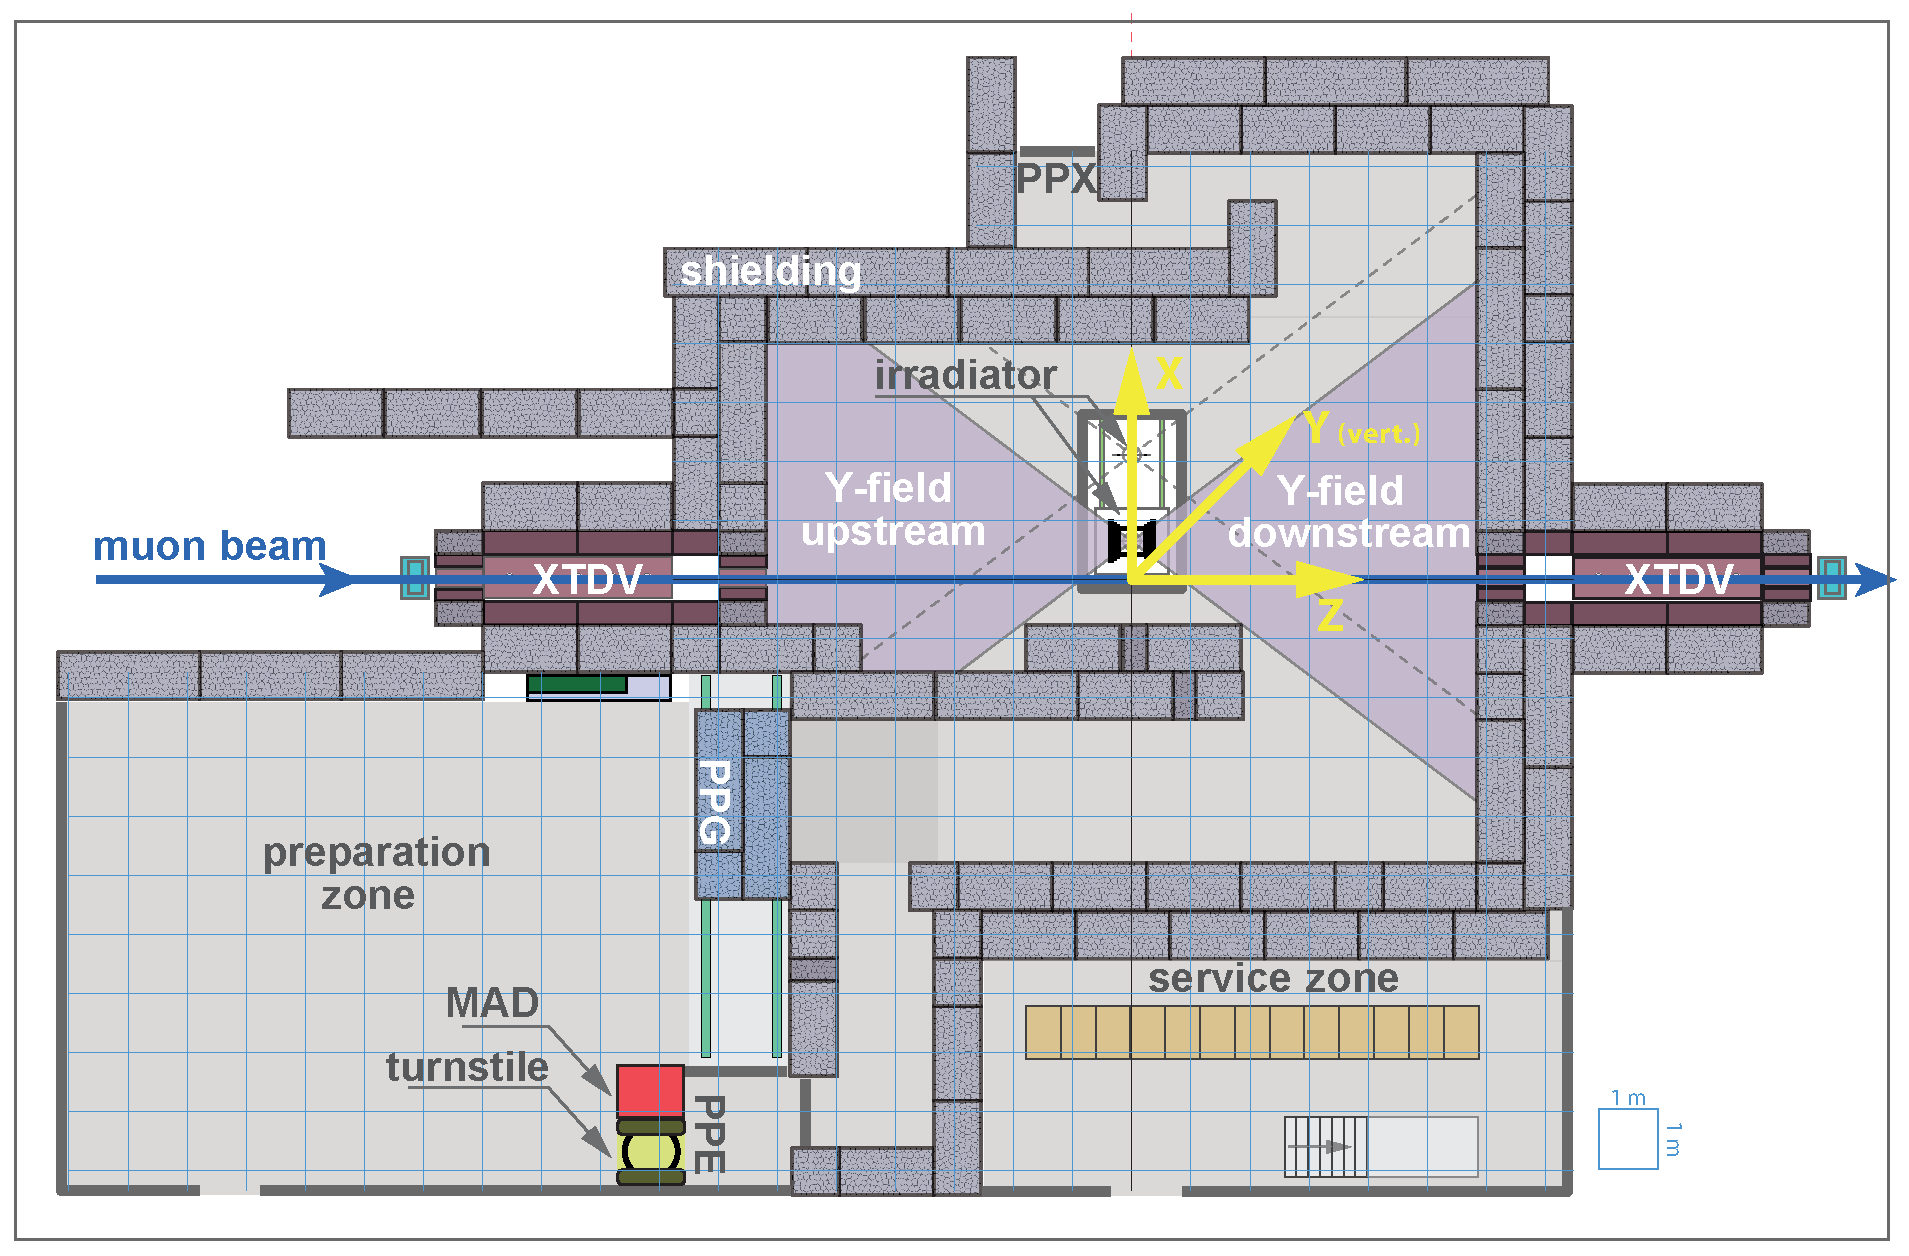
\includegraphics[scale=0.35]{fig/wincc/GIF.pdf}
  \caption{An overview of the GIF++ with entrance doors MAD (material access door), PPG (personal protection gate), PPE (personal protection entrance), PPX (personal protection exit).}
\label{fig:gif}
\end{figure}
The radiation field is uniformly distributed over the xy-plane as required for large-area flat detectors with the help of two $\pm \ang{37}$ angular correction filters both in the downstream and upstream regions. It is shown in Fig.~\ref{fig:attenuator_gif}a. The photon current is fine-tuned using two complete and independent attenuation systems. It consists of 3$\times$3 convex lead filters and attenuates photons that have energy less than 662\,keV to a higher degree. The attenuator system is shown in Fig.~\ref{fig:attenuator_gif}b with three planes (A, B, C) on either side of the source, and each plane further consists of three filters. Each filter possesses the nominal attenuation factors; 1 (A1,B1,C1), 1.5 (B2), 2.2 (C2), 4.6 (C3), 10 (A2), and 100 (A3, B3). A set of 24 nominal attenuation factors (nearly equidistant) have been selected from the 27 combination of 3$\times$3 that varies from 1 to 46415 as shown in Fig.~\ref{fig:attenuator_gif}c.  
\begin{figure}[htp]
\centering
\begin{tabular}{ccc}
\hspace{-0.2cm}
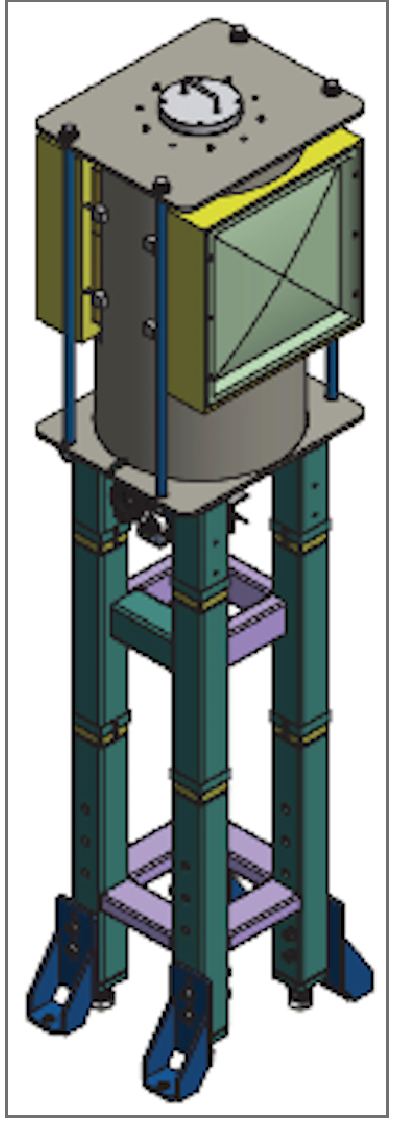
\includegraphics[scale=0.5]{fig/wincc/irradiator.pdf}
& \hspace{-0.632cm} 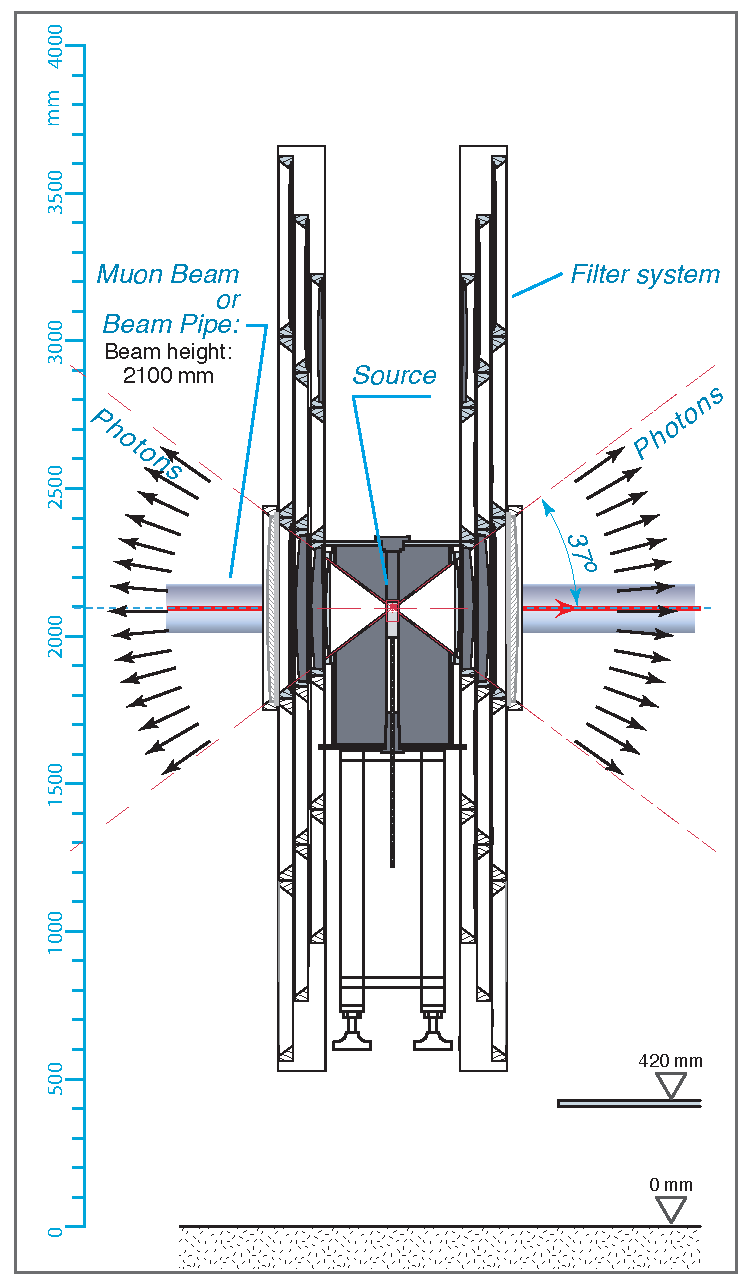
\includegraphics[scale=0.443]{fig/wincc/filters.pdf}
& \hspace{-0.65cm} 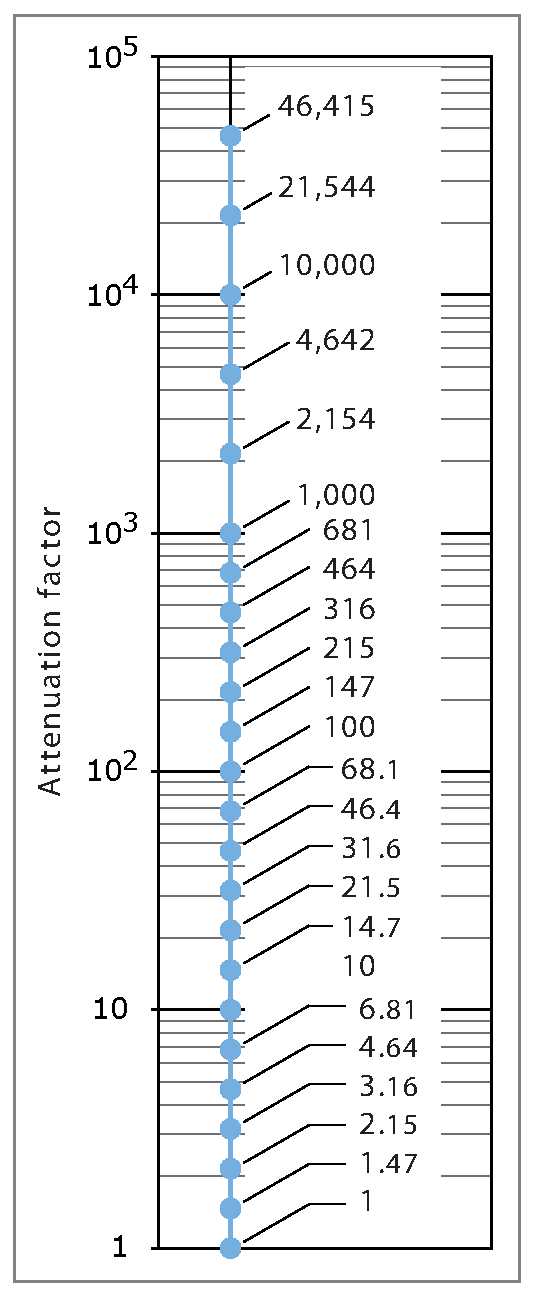
\includegraphics[scale=0.439]{fig/wincc/filter_factors.pdf}\\
  \qquad ($\mathbf{a}$)\qquad\qquad&($\mathbf{b}$)\qquad\qquad&($\mathbf{c}$)\\
\end{tabular}
\caption{Irradiator with the attenuator system in the GIF++. (a): Irradiator with independent angular correction filters on both sides. (b): Irradiator with remotely controlled attenuation filters to vary the radiation intensity. (c): A set of 24 nominal attenuation factors are selected from the 27 combination (3$\times$3) that varies from 1 to 46415.}\label{fig:attenuator_gif}
\end{figure}

Simulation of the 662\,keV photon current is shown in Fig.~\ref{fig:gif_simul} using an attenuator factor 1 (unattenuated). Using the angular correction filters, the current is uniformly distributed along the y-axis and varies from the source along the z-axis. 
\begin{figure}[h]
\centering
 \includegraphics[scale=0.55,trim=0 0 0 0,clip]{fig/wincc/Current_gifpp_DS_US_flatSurfaceCurrent_600_662_x_60_70.pdf}
 \caption{Simulation of the unattenuated 662\,keV photon current in the yz-plane at x = 0.65\,m; using the angular correction filter.}
\label{fig:gif_simul}
\end{figure}

Table~\ref{tab:att_values} displays the nominal attenuation of 662\,keV photons and dose attenuation measured with the Automess gamma probe 6150AD-15 for different filter combinations. For factors less than 10, the nominal and effective dose attenuations are comparable while for greater than 10, the effective dose attenuation is considerably lower than the nominal attenuation factor, since scattered photons with an energy smaller than 662\,keV contribute substantially. 
\begin{table}[h]
\centering
\begin{tabular}{cc|c|c|}
\cline{3-4}
& & \multicolumn{2}{ c| }{Measured data} \\
\cline{1-4}
\multicolumn{1}{ |c|  }{Nominal} & Filter & Dose Rate & Dose \\
\multicolumn{1}{ |c|  }{Attenuation} & Combination & [mGy/h] & Attenuation \\ \cline{1-4}
\multicolumn{1}{ |c|  }{1 }      & A1 B1 C1 &   470.00   & -    \\ 
\multicolumn{1}{ |c|  }{1.5 }    & A1 B2 C1 &   400.00   & 1.2   \\
\multicolumn{1}{ |c|  }{2.2 }    & A1 B1 C2 &   211.00   & 2.2    \\
\multicolumn{1}{ |c|  }{4.6 }    & A1 B1 C3 &   105.00   & 4.5    \\
\multicolumn{1}{ |c|  }{10  }    & A2 B1 C1 &   55.00    & 8.8    \\
\multicolumn{1}{ |c|  }{100 }    & A3 B1 C1 &   6.50     & 72.3   \\
\multicolumn{1}{ |c|  }{100 }    & A1 B3 C1 &   6.20     & 75.8   \\
\multicolumn{1}{ |c|  }{464 }    & A1 B3 C3 &   1.59     & 295.6  \\
\multicolumn{1}{ |c|  }{4642}    & A2 B3 C3 &   0.22     & 2156.0 \\
\multicolumn{1}{ |c|  }{46415}   & A3 B3 C3 &   0.05     & 9400.0 \\ \cline{1-4}
\end{tabular}
  \caption{Nominal attenuation factors (attenuation of the 662\,keV photons) of some filter settings and measured effective attenuation in position D1 (x=0.65\,m, y=0.00\,m, z=1.10\,m)}
  \label{tab:att_values}
\end{table}

At the GIF++, the RPC detectors setup consists of two endcap chambers of type RE2 and RE4 that are continuously irradiated. Two non-irradiated chambers of the same type are installed to be used as reference. They are accompanied by the new generation of Glass-RPC (GRPC)~\cite{1748-0221-11-09-C09006} and multi-gap RPCs. A dedicated control system has been built to control these detectors and archive the relevant parameters using the WinCC-OA (PVSS) Supervisory Control And Data Acquisition (SCADA) system~\cite{twiki:wincc-oa}. The system controls high as well as low voltage supplies and monitors temperature, pressure, and humidity for both the RPC gas and the environment. The source status and attenuator values are accessed using the data interchange protocol (DIP), which is published centrally by the Engineering Department. The RPC gas supply is controlled and monitored by an external WinCC-OA project that shares relevant parameters with this project. All the relevant parameters are archived in a Structured Query Language (SQL) database (DB) for offline analysis.

One of the features of the GIF++ RPC DCS system is accessing the source status and attenuator values, as shown in Fig.~\ref{fig:attenuator_gif}c. Based on this information, the RPC performance parameters (efficiency, working point, cluster size, and resistivity) are measured. To retrieve the data from the database, a specific algorithm has been developed to synchronize the detector parameters (current and voltage) with the external parameters (temperature, pressure, and humidity). It enables the precise monitoring of the effect the external parameters have on the detector.
\section{WinCC-OA}\label{sec:wincc}
The SCADA System SIMATIC WinCC-OA~\cite{wincc_oa} is designed by ETM of the Siemens group and used extensively in large industries to supervise and control complex processes. Large experiments at CERN use the commercial ETM SCADA software, WinCC-OA, as a tool to develop control systems. WinCC-OA is consistently built on object-oriented structures, supported by both Windows and Linux systems, is flexible as well as distributed, and has an open architecture. 
WinCC-OA has the ability to connect hardware (or software) devices under a particular Detector Control System (DCS) and archive their data to observe the behaviour of the device under consideration. WinCC-OA describes a device in terms of a data point in a tree-like structure, with data point elements representing the device parameters. These can then be addressed directly to write to and read from the corresponding device. 
The WinCC-OA software runs different processes called ``Managers''. Event Manager (EV) is the heart of a WinCC-OA system, which connects other specific tasks managers. Figure~\ref{fig:wincc_managers} shows these managers and their specific functions. 
\begin{figure}[h]
\centering
 \includegraphics[scale=0.4,trim=0 0 0 0,clip]{fig/wincc/winccOA_manager.jpg}
 \caption{The concept of managers in WinCC-OA and it's functional layers. The event manager plays a key role in connecting all managers in a tree-like structure~\cite{wincc_managers}.}
\label{fig:wincc_managers}
\end{figure}

WinCC-OA is capable of building a distributed system in such a manner that different projects get interconnected and can exchange information remotely via the TCP/IP protocol using a ``Distribution'' Manager.
WinCC-OA uses a number of Managers as ``Drivers'' to communicate with the Front End (FE) hardware for data readout by mostly using the industry standard protocols, such as Profibus, CanBus, DIM, and Modbus, for communicating with the Programmable Logic Controllers (PLC) and OPC servers.
In order for non-experts to easily and safely operate the system, WinCC-OA provides a user-friendly Graphic User Interface (GUI) panel – an intuitive tool for controlling, monitoring, and operating the detectors in the safe mode. It provides the flexibility to combine text, graphical objects, and synoptic diagrams. The GUI panels can be used to observe the online behaviour of the detector in the form of plots, tables, and histograms. An example of the GUI is shown in Fig.~\ref{fig:gui}.
\begin{figure}[h]
\centering
\includegraphics[scale=0.5,trim=0 175 10 80,clip]{fig/wincc/GUI2.png}\\
 \caption{FSM main tree and high voltage scan panel using GUI.}
\label{fig:gui}
\end{figure}

All the LHC experiments have common tasks and requirements; therefore, it is necessary to have a general framework to provide all the required standard features and facilities. The Joint Controls Project (JCOP)~\cite{jcop} was developed to reduce the repetition of efforts by reusing common components and concealing the complexity of the underlying tools. The JCOP framework provides extra functions such as standardized Finite State Machine (FSM), the additional Graphical User Interface (GUI), the alarm handlers, and the ORACLE database interface~\cite{g-polese}.
The JCOP framework provides FSM toolkits in WinCC-OA based on State Machine Interface (SMI++). It offers an easy, robust, and safe way to control the full detector through the definition of a finite number of states, transitions, and actions (ON, OFF, STANDBY, Ramping Up, Ramping Down). A typical device state for an HV channel is implemented through the FSM mechanism, as shown in Fig.~\ref{fig:hierarchy}.
\begin{figure}[H]
\centering
\hspace{-0.5cm}
\includegraphics[scale=1.5,trim=160 600 160 120,clip]{fig/wincc/hierarchy.pdf}\\
 \caption{The DCS hierarchy tree for a typical high voltage channel using FSM. The tree shows a transition from one state to another.}
\label{fig:hierarchy}
\end{figure}
\section{The CMS RPC DCS project at GIF++}\label{sec:rpc_proj}
The CMS RPC DCS at GIF++ has been developed using WinCC-OA 3.11 and extended using the standard JCOP framework. It is designed in a tree-like structure with sub-systems of High Voltage (HV), Low Voltage (LV), environmental, and gas parameters (pressure, temperature, and humidity) as well as radiation levels. Each sub-system is mainly divided into two parts, the Front-End (FE) hardware located around the experimental area (sensors, power supplies, etc.) and a Back-End (BE) computer network wherein the DCS is running. The HV and LV power supplies used in the RPC GIF++ setup consist of CAEN SY1527 mainframe modules as well as CAEN EASY modules, with additional ADC modules used to read gas and environmental sensors (pressure, temperature, and humidity). The project has access to the hardware registered through Object Linking and Embedding (OLE) for Process Control (OPC) server provided by CAEN using the OPC protocol~\cite{opc}. The project controls the HV and LVsystem using the OPC protocol. The environmental and gas sensors (for pressure, temperature, and humidity) are also read out using the OPC protocol. The source status and attenuator values are available centrally via the DIP. The project has been designed to be distributed in order to enable communication with other projects and to read valuable information. Communication is established with the central GIF++ DCS in such a manner that the information from the gas system, such as flow rates, are readable.\\
The FSM hierarchy of the project is based on the naming convention of the trolley, where the detectors are installed. Each trolley has six sections and each section accommodates one detector. Currently, three CMS RPCs trolleys are installed in the GIF++. Trolley~1 (RPC Consolidation) is equipped with spare RPCs, trolley~2 with small glass RPCs, and trolley~3 with prototypes of improved RPCs. Figure~\ref{fig:rpc_setup} shows the RPCs configuration in a trolley, and detailed information of the trolleys are provided here~\cite{salvador}. 
A schematic overview of the DCS project is shown in Fig.~\ref{fig:DCS_sys}.
\begin{figure}[h]
\centering
\includegraphics[scale=0.4,trim=60 30 60 30,clip]{fig/wincc/DCS_sys.png}\\
 \caption{An overview of the CMS RPC DCS at the GIF++.}
\label{fig:DCS_sys}
\end{figure}
\subsection{High and low voltage system}
The power supply system provided both HV and LV to the installed RPCs in the GIF++. Owing to the simple setup, both the HV and LV boards were installed in the CAEN mainframe that are located outside the radiation zone.
The high and low voltage system is controlled and monitored by the CAEN OPC server. Each gap in a chamber is independently connected to a single high-voltage channel, which improves the granularity of control. The RPC front-end electronics requires digital and analogue power supplies~\cite{feb}. Each low-voltage line has been shared between the two front-end-boards (FEBs) for digital as well as for analogue power supply. The DCS communication with the CAEN mainframe is shown in Fig.~\ref{fig:caen_control}
\begin{figure}[h]
\centering
\includegraphics[scale=1.0,trim=60 380 60 320,clip]{fig/wincc/caen_control.pdf}\\
 \caption{The HV and LV channels can be operated by the CAEN mainframe independently, and the DCS is connected to the CAEN via OPC server. An easy crate is used for environmental and gas parameter measurement.}
\label{fig:caen_control}
\end{figure}
\subsection{Environmental and gas parameters}
The performance of the RPCs strongly depends on the temperature and pressure of the environment because the RPC's gas density is directly affected by these parameters. Hence, it is important to measure the environmental parameters (temperature, pressure, and humidity) at different locations where the RPCs are installed. The applied voltage is corrected for the environmental temperature and pressure in order to include their effects using Eq.~\ref{equ:temp_press_correc}:  
\begin{equation}\label{equ:temp_press_correc}
HV_{app}(P, T) = HV_o . \frac{P_o}{P}\frac{T}{T_o}
\end{equation} 
Where $P_o$, $T_o$ are the environmental and $P$, $T$ are the bunker (the radiation zone) pressures and temperatures respectively. $HV_o$ is the user set-up high-voltage and $HV_{app}$ is the corrected high voltage supplied by the DCS system.
This procedure is described in detail in~\cite{env-rpc}. 
Figure~\ref{scan_temp}a provides a plot for the environmental temperature, pressure, and humidity. The environmental and gas sensors (temperature, pressure and humidity) are readable through the ADC (analog-to-digital converter) board that is installed in the EASY crate. The JCOP framework presents the opportunity to convert the ADC counts into physical values online. The trending feature provides a comparison between different sensors located at different positions.
\subsection{High voltage scan and stability test}
The project has been designed for the R\&D of detectors. Hence, it should be able to perform high-voltage scanning or stability tests. For high-voltage scanning, a separate branch has been incorporated in the FSM tree, wherein the user operates each detector independently. 
A typical UI panel used for HV scanning is shown in Fig.~\ref{fig:gui}(right). Using this panel, a user can select different voltage values (left column), a single current value (second left column), and operate detectors independently (third column). The user has access to mask a single HV channel (connected to a specific part of the RPC detector) without making the whole detector. 
The stability test runs for a long period of time in order to expose the detectors to high radiation. Based on the requirements, a dedicated manager applies the stability script and restarts it automatically. An example of a HV scanning plot for one of the CMS RPC chambers (RE3) at GIF++ is shown in Fig.~\ref{scan_temp}b. 

\begin{figure}[h]
\centering
\begin{tabular}{cc}
\hspace{-0.3cm}
\includegraphics[scale=0.33,trim=50 70 20 90,clip]{fig/wincc/tprh.png}
& \hspace{-0.5cm} \includegraphics[scale=0.345,trim=50 100 45 80,clip]{fig/wincc/HV_Scan2.png}\\
   ($\mathbf{a}$)\qquad&($\mathbf{b}$)\qquad\\
\end{tabular}
\caption{(a): Environmental temperature ($^o$C), pressure (mb), and humidity (\%). Time is on the x-axis while the red, blue, and green lines represent the values of pressure, temperature, and humidity respectively on the y-axis. The pressure and temperature values used for operating voltage correction of the RPCs. (b): A HV scan of the CMS RE3 chamber. The x-axis shows time while the y-axis shows the voltage (V) and current ($\mu$A) values. The red, blue, and green lines are voltages while the cyan, brown, and orange lines are the corresponding current values for bottom, top-narrow, and top-wide gaps respectively.}\label{scan_temp}
\end{figure}

\subsection{Database}
To study the behaviour of the detector over time and to perform an offline data analysis, it is necessary to store all the important parameters in a database. In particular, the HV, LV, environmental and gas parameters, and radiation levels (attenuator values) are kept for this purpose. This information can be utilized to constantly check the online behaviour of a detector during operation and for the offline analysis to measure the ageing effects after it has absorbed a specific radiation dose. WinCC-OA's uses an internal database for small and simple projects, which stores data locally on the hard drive or on an external oracle database for more complex technical processes that generate large quantities of data. The Relational Database Manager (RDB) is specifically assigned to archiving data in the external oracle database. 

Compared to the central CMS RPC system, the RPCs at the GIF++ generate a small amount of data; hence, we used the internal built-in SQL database in this project. It doesn't need the RDB manager to run. The data point is archived in the database when a change occurs in its value. To suppress the noise fluctuation and reduce the size of data, a ``deadband'' is specified for each archiving parameter. Since the changes in environmental parameters and HV don't occur at the same time, the values stored in the database are not synchronized. A specific algorithm is applied to synchronise all the relevant stored parameters for analysis. The stored data is finally extracted to be used for the offline analysis using a GUI.


\section{CMS RPC longevity studies}
RPCs are gaseous detectors and in principle can suffer from ageing effects when exposed to a prolonged radiation that deteriorates the detector performance in the form of efficiency loss, dark rate, dark current etc. The deterioration is mainly caused by complicated chemical processes largely occurring in the hot plasma inside electron multiplication avalanches where gas molecules may form polymers growing on electrodes. The severity of ageing increases with integral of radiation exposure and depends on a myriad of factors, such as detector geometry, the materials used for the electrodes, operational gas gain, gas mixture, impurities in the gas itself, gas flow rate etc. 
For the life span of an experiment, the ageing effects of the installed detectors can be studied by subjecting the same detectors prototypes to accelerated ageing tests performed at a higher instantaneous radiation rate. Assuming the dependency of detector's ageing on the accumulated charge per unit area (in case of RPC), the obtained results from these tests can be projected towards many years of operation at the expected nominal radiation. Since this is approximation and quantitatively not productive, so a large safety margin factor of 3 is used to accumulate the total amount of radiation precisely. The performance of the installed CMS RPC system has already been certified for 10~LHC years in the GIF facility at maximum background rate of 300\,Hz-cm$^{-2}$ and a total integrated charge of 50\,mC-cm$^{-2}$~\cite{ABBRESCIA2004102}.

The background rates showed linearly dependency on the instantaneous luminosity during the Run-I and Run-II data taking periods both in barrel as well as in endcap regions. Assuming the same linear relationship, the expected rates are extrapolated to the HL-LHC conditions reaching up to 600\,Hz-cm$^{-2}$ including a safety factor of 3, as shown in Fig.~\ref{fig:cms_rpc_extrapolated_rates} for all barrel (left) and endcap (right) chambers. Using the same safety factor, the expected integrated charge in the hottest region of the current RPC system will be 840\,mC-cm$^{-2}$ at the end of the HL-LHC. The same amount of integrated charge will be accumulated in the GIF++ facility to certify the detectors for HL-LHC conditions. 
  
\begin{figure}[h]
\centering
\includegraphics[width=0.49\textwidth,keepaspectratio=true]{fig/wincc/longevity/Barrel-Roll-Rate-HL-LHC.pdf}
\includegraphics[width=0.49\textwidth,keepaspectratio=true]{fig/wincc/longevity/Endcap-Disks-Rate-HL-LHC.pdf}
\caption{Extrapolation from 2016 data of single hit rate per unit area to HL-LHC conditions, in the barrel (left) and endcap (right) regions, for the present RPC system.}
\label{fig:cms_rpc_extrapolated_rates}
\end{figure}

The longevity study has already been started in the GIF++ facility by continuously irradiating the two turned on chambers, RE2/2 and RE4/2. The total integrated charge accumulated by the two chambers are shown in Fig.~\ref{fig:gifpp_integrated_Q}. At the end of 2017, the total integrated charge for RE2/2 and RE4/2 was about 292\,mC-cm$^{-2}$ and 119\,mC-cm$^{-2}$ respectively which corresponds to 34\% and 14\% of the expected integrated charge at the HL-LHC. Due to gas flow limitation, the RE4/2 was turned on later.   
\begin{figure}[h]
\centering
\includegraphics[width=0.59\textwidth,keepaspectratio=true]{fig/wincc/longevity/GIFPP_Integrated_Charge.pdf}
\caption{Integrated charge versus time accumulated during the GIF++ studies for the RE2/2 (red) and RE4/2 (blue) chambers. Because of total gas flow limitations, the RE4/2 chamber has been turned on few months later. Different slopes account for different irradiation conditions during data taking.}
\label{fig:gifpp_integrated_Q}
\end{figure}

\subsection{RPCs setup at GIF++ for efficiency studies}\label{eff_calc}
Four RPC chambers (two RE2 and two RE4~\cite{feb}) are placed parallel to each other in a vertical position, a few meters away from the source in the upstream area as shown in Fig.~\ref{fig:rpc_setup}.
\begin{figure}[h]
\centering
\includegraphics[scale=0.07]{fig/wincc/RPC_setup.jpg}\\
 \caption{CMS RPCs setup in the GIF++. Detectors are placed perpendicularly and a few meters away from the source.}
\label{fig:rpc_setup}
\end{figure}
Several high-voltage scans were performed using different radiation levels (starting from the absence of radiation source) to define the optimal operating voltage of each chamber, which is called Working Point (WP). The efficiency (E) for different background radiation levels is calculated using the equation:
\begin{equation}
 {E = N_{RPC}/N_{TRACK}.}
\end{equation}
The muon track is reconstructed using three reference RPC planes and extrapolated to the RPC under test, examining the closest cluster (a strip or set of continuous strips). N$_{TRACK}$ corresponds to the number of muons passing through the three reference RPC detectors at the same time. N$_{RPC}$ corresponds to the number of fired clusters in the chamber under test. The dependence of the efficiency E on the effective high voltage HV$_{eff}$~\cite{hv-eff} can be fitted using the following sigmoidal curve:
\begin{equation}
{\langle E\rangle = E_{max} / (1 + exp (-\lambda (HV_{eff} - HV_{50\%})),}
\end{equation}
where E$_{max}$ is the maximum efficiency reached by the chambers at HV$\rightarrow \infty$, $\lambda$ is proportional to the slope of sigmoid at flex point, and HV$_{50\%}$ is the high voltage at which a chamber reaches 50\% of its maximum efficiency. The Working Point of a chamber is defined by:
\begin{equation}
 HV_{wp} = HV_{knee} + 150V,
\end{equation} 
where HV$_{knee}$ is the voltage at which the efficiency is 95\% of the maximal one.   

\subsection{Efficiency and cluster size results}
In Fig.~\ref{eff}a, the efficiency as a function of HV$_{eff}$ for different radiation levels is presented. The maximum efficiency slightly decreases with the amount of radiation received by the detector. In Fig.~\ref{eff}b, the maximum efficiency as a function of the gamma hits rate is presented for four RPC chambers. The RPCs were placed parallel to each other, with RPC-1 being the closest to the source while RPC-4 was the furthest. The radiation dose depends on the distance between the RPCs and the gamma source. RPCs 3 and 4 received a smaller dose as compared to RPCs 1 and 2. 
\begin{figure}[h]
\centering
\begin{tabular}{cc}
\hspace{-0.5cm}
\includegraphics[scale=0.30,trim=0 13 0 0,clip]{fig/wincc/eff.png}
& \hspace{-0.60cm} \includegraphics[scale=0.329,trim=0 0 0 0,clip]{fig/wincc/rate_eff.png}\\
   ($\mathbf{a}$)\qquad&($\mathbf{b}$)\qquad\\
\end{tabular}
\caption{(a): Efficiency vs HV$_{eff}$ for different gamma attenuator factors. (b): Maximum efficiency vs gamma rate at HV$_{wp}$ for four RPCs.}\label{eff}
\end{figure}

Figure.~\ref{eff} represents the very first results obtained in the GIF++ at the start of 2016. Afterwards, several measurements have been performed under different background radiation conditions using the dedicated attenuator system. Each time the detector performance has been studied. Figure~\ref{fig:cms_rpc_eff_diff_periods} shows the hit efficiency of the RE2/2 chamber as a function of the effective HV at different irradiation stages, corresponding to an integrated charge of 0, 153\,mC-cm$^{-2}$ and 257\,mC-cm$^{-2}$. The background radiation rate is minimum (source-off) in the left plot and maximum (about 600\,Hz-cm${-2}$) in the right plot. The detector showed stable behaviour over time and no change in the efficiency and working point has been observed.    

\begin{figure}[h]
\centering
\includegraphics[width=0.49\textwidth,keepaspectratio=true]{fig/wincc/longevity/RE2-Efficiency.pdf}
\includegraphics[width=0.49\textwidth,keepaspectratio=true]{fig/wincc/longevity/RE2-Efficiency-600.pdf}
\caption{Hit efficiency of RE2/2 as a function of the effective HV, without irradiation (left) and under a gamma background rate of about 600\,Hz-cm$^{-2}$ (right). The measured efficiency of the RE2/2 chamber corresponds to different Test Beams (TB) with integrated charge: 0, 153\,mC-cm$^{-2}$ (18\%) and 257\,mC-cm$^{-2}$ (31\%). The detector performance is stable at high fraction of accumulated charge.}
\label{fig:cms_rpc_eff_diff_periods}
\end{figure}

A similar study has been done to monitor the cluster size, defined as the number of fired strips per hit. Figure~\ref{fig:cms_rpc_cluster_diff_periods} shows the cluster size as a function of effective HV for RE2/2 chamber with integrated charge: 153\,mC-cm$^{-2}$ (18\%) and 257\,mC-cm$^{-2}$ (31\%) without background radiations (left) and background gamma irradiation of about 600\,Hz-cm$^{-2}$ (right). No significant change has been observed in the cluster size.

\begin{figure}[h]
\centering
\includegraphics[width=0.49\textwidth,keepaspectratio=true]{fig/wincc/longevity/RE2-ClusterSize.pdf}
\includegraphics[width=0.49\textwidth,keepaspectratio=true]{fig/wincc/longevity/RE2-ClusterSize-600.pdf}
\caption{Cluster size of RE2/2 as a function of the effective HV, without irradiation (left) and under a gamma background rate of about 600\,Hz-cm$^{-2}$ (right). The measured cluster size of the RE2/2 chamber corresponds to different Test Beams (TB) with integrated charge: 153\,mC-cm$^{-2}$ (18\%) and 257\,mC-cm$^{-2}$ (31\%). The cluster size is above 2 at working point of the detector with high fraction of accumulated charge.}
\label{fig:cms_rpc_cluster_diff_periods}
\end{figure}

\section{Summary} 
The DCS project for the CMS RPCs has successfully been implemented and tested in the CERN GIF++. Since June 2015, the project has been running in a stable manner. The detectors are being operated and the data being archived. The hardware integrated in the project fully controls the high-voltage scanning and stability tests. Environmental and gas sensors are included and used for temperature and pressure corrections. Gas flow-meters are read through the central DCS at GIF++, and the data is used to study the behaviour of different gas mixtures. All useful parameters are archived in the internal database for offline analysis. As the project is designed for detector R\&D studies, any new hardware can be added easily and safely.

The performance of the CMS RPC chambers at GIF++ has been studied and compared at different radiation levels. At a rate of 600\,Hz-cm$^{-2}$, the Eff$_{max}$ of the chamber was 95\%. 
The detectors showed stable performance up to 34\% of the expected integrated charge that will be accumulated at the end of the HL-LHC run. 
%\acknowledgments We wish to congratulate our colleagues in the CERN Engineering- (EN) and Physics- Department (PH) for successful operation of the GIF++. We thank the technical and administrative staff at CERN, other CMS institutes and RPC group. Many thanks to ATLAS colleague Marino Romano for his technical support to develop the project.   



%\renewcommand*{\thesection}{\thechapter.\arabic{section}}       % reset again to chaptnum.sectnum

%\clearpage{\pagestyle{empty}\cleardoublepage}

\graphicspath{{chapt_dutch/}{intro/}{chapt2/}{chapt3/}{chapt4/}{chapt5/}{chapt6/}{chapt7/}{chapt8/}}

% Header
\renewcommand\evenpagerightmark{{\scshape\small Chapter 5}}
\renewcommand\oddpageleftmark{{\scshape\small Monte Carlo Simulation and Event Reconstruction}}

\renewcommand{\bibname}{References}

\hyphenation{}

\chapter[Monte Carlo simulation and event reconstruction]%
{Monte Carlo Simulation and Event Reconstruction}\label{chapt:5}
This chapter describes the Monte Carlo (MC) simulation methods used in the field of high-energy physics for signal and background process generation. It explains in detail the particle physics generators that are used in the analysis included in this thesis. Event and physics objects reconstruction in the CMS detector are described in the last two sections. 
\section{Monte Carlo simulation}\label{sec:mc_sim}
In high-energy physics experiments, event modelling plays an important role to understand the collected data. A precisely modelled event maximizes the chance of discovering new physics and making precision measurements of the Standard Model (SM) processes. However, in hadron-hadron colliders where the colliding particles are composite objects, like proton-proton in LHC, event modelling is a challenging task. The same applies to particle interactions within the bulk of the detector volume. These tasks can be solved by employing Monte Carlo generation techniques, and incorporating the SM models of new physics as well as the detector effects while detecting the final-state particles in the interaction. An event occurs when two protons collide and produce a cascade of new particles as shown in Fig.~\ref{fig:event}. Because of the complexity of the event, the MC generators model the events in a simulation chain: Hard interaction, parton showering, hadronization, and decays. These processes are explained in the following sections.
\begin{figure}[h]
\centering
%\captionsetup{width=0.8\linewidth}
\includegraphics[width=0.6\textwidth]{fig/chapt4/event_sim.jpeg}
%\includegraphics[scale=0.4, trim=20 50 60 30,clip]{fig/chapt3/CMS_exper.png}
\caption{\label{fig:event}The pictorial representation of a $pp$ collision event~\cite{simulated_event}. The hard interaction is represented by the big red blob. Additional hard QCD radiation is produced (red) and a secondary interaction takes place (purple blob) before the final-state partons hadronise (light-green blobs) and hadrons decay (dark green blobs). Photon radiation occurs at any stage (yellow)}.
\end{figure}  
\subsection{Parton distribution functions}
In hadron colliders such as the LHC, the colliding particles (protons) have a composite structure consisting of gluons and quarks. In this analysis, the SM $t\bar t$ and the heavy Higgs (H, A) states are produced by the gluon fusion. Therefore, it is necessary to understand the internal structure of proton, described by the \textit{Parton Distributing Functions (PDFs)}. The parton density function $f_{i}(x, Q^2)$ gives the probability of finding a parton (quarks or gluons) of flavour $i$ in the proton, carrying a fraction $x$ of the proton momentum with $Q$ being the energy scale of the hard interaction~\cite{Placakyte:2011az}. An accurate determination of PDFs, and their corresponding uncertainties is obtained from global fits to a variety of data from multiple experiments, such as HERA, Tevatron, and LHC, using the DGLAP evolution equation. These results show that for small values of $Q^2$, a large fraction of the hadron momentum is carried by its valence quarks; whereas at high energies, most of the hadron momentum is carried by the so-called sea partons, i.e. gluons and virtual $q\bar q$ pairs.

This analysis uses the ``\textsc{nnpdf30}” sets provided by the ``\textsc{nnpdf}” collaboration~\cite{nnpdf_sets}. ``\textsc{nnpdf}” uses an unbiased modelling tool, Neural Networks, with trained genetic algorithms to construct a Monte Carlo representation of PDFs and their uncertainties – a probability distribution in a space of functions. As a final user, a set of 100 MC replica has been used to compute PDF-dependent quantities along with their uncertainties. The central value represent the ``best fit'' PDF, while the error members represent variations around the best result. The PDF uncertainties are discussed in detail in Sec.~\ref{subsec_theo_uncer}.



\subsection{Hard scattering}
The actual interaction of two protons occurs when partons from the two colliding protons interact and produce new particles with high $p_{T}$. These events are of keen interest for analysis and are referred to as hard scattering. If the colliding protons merely undergo soft collision, the resultant particles have low $p_{T}$, commonly known as soft scattering. PDFs describe the structure of the proton and contain the initial momentum distribution of the partons involved in the hard interaction. In hadron-hadron (in case of LHC, it is $pp$) collisions, a wide variety of hard scattering cross sections can be calculated using the QCD factorization theorem and weighting the subprocess cross section with the PDFs extracted from deep inelastic scattering~\cite{hard_scatter}. Factorization theorems separate long- and short-distance physics when calculating these cross sections.   
\begin{equation}\label{eq:xsec}
\sigma_{AB} = \int dx_{a}dx_{b}f_{a/A}(x_{a},\alpha_{s},\mu_{F}).f_{b/B}(x_{b},\alpha_{s},\mu_{F}).\hat{\sigma}(\hat{s};\alpha_{s},\mu_{F},\mu_{R})
\end{equation}  
Where, $f_{a/A}$ is the probability that a parton $a$ inside a hadron $A$ carries a momentum fraction $x_{a}$, $\hat{s}$ is the parton centre-of-mass energy, $\alpha_{s}$ is the strong coupling constant, $\mu_{F}$ is the factorization, and $\mu_{R}$ is the renormalization scale.

\subsection{Particle physics generators}\label{sec:gnerators}
In the current High Energy Physics (HEP) regime, the most challenging aspect is the multiparticle production, where the observed particle multiplicities extend to hundred. These multiplicities are expected to go upward in future HEP colliders. Event Generators (EG), based on computer programs, solve this problem by generating events as detailed as could be observed by a perfect detector.   
In High Energy Physics, a number of Monte Carlo (MC) generators are available to calculate the tree-level diagrams numerically and integrate them over the relevant phase space. A list of them are used in Monte Carlo production for this analysis is discussed below.
\begin{itemize}
\item\textsc{MadGraph:} now merged into \textsc{Mg\_amc@nlo}, a general-purpose event generator~\cite{madgraph} used for the generation of signal samples in this analysis. It is a pure-matrix element generator that generates hadron-hadron ($pp, p\bar{p}, gg, q\bar{q}$) collision and in practice, produces eight particles (quarks, gluons, and leptons) in the final state without hadronization. It also provides an opportunity to produce samples using the interference effect. The interference comes into play when the signal and background have the same final state particles; in this analysis, the signal $gg\rightarrow H/A \rightarrow t\bar{t}$ and the SM $t\bar{t}$, the main background, have same final state particles. 
\textsc{MadGraph} is further interfaced with \textsc{Pythia} or \textsc{Herwig} to generate showering and hadronization steps. The double counting in the showering is solved by applying the MLM scheme. To describe the parton structure, ``\textsc{nnpdf30}'' PDF~\cite{pdf_sets} sets are used in this analysis. 

\item{\textsc{Pythia:}}\label{subsec:pythia} is a multipurpose event generator used frequently in HEP. It provides the possibility to generate complete events in as much detail as experimentally observable within the bounds of our current understanding of the underlying physics. \textsc{Pythia} is used to model $e^{+}e^{-}$, $ep$ and $pp$ collisions and simulate a large variety (over 300) of hard 2 $\rightarrow$ 2 processes that include SM and many BSM processes up to Leading Order (LO) accuracy. \textsc{Pythia} uses the Lund string model~\cite{lund_string_model} to describe hadronization and external PDFs for hard processes calculations. It uses a $p_{T}$-ordered showering technique for parton showering, where partons are ordered by their transverse momentum ($p_{T}$) and $Q^{2} = p^{2}_{T}$ – the closer the parton is to the vicinity of the hard process, the higher $p_{T}$ is assigned to it. More detail about the \textsc{Pythia} program is given in~\cite{pythia}.

\item{\textsc{Powheg:}} PositiveWeight Hardest Emission Generator is an event generator~\cite{powheg} that provides modelling of the hardest interaction at NLO QCD accuracy and needs to be interfaced with \textsc{Pythia} or \textsc{Herwig} for the parton showering and hadronization. The proton structure is described using the PDF sets \textsc{nnpdf30} for the MC samples generated by \textsc{Powheg}.

\item{\textsc{Mc@nlo:}} is an event generator~\cite{mcanlo} that generates hard emissions using NLO fixed-order QCD calculations with the (N)LL accuracy shower algorithm implemented in \textsc{Herwig}. For showering hadronization and decays, the \textsc{Mc@nlo} has to be interfaced with a general-purpose detector such as \textsc{Herwig} or \textsc{Pythia}. The event generation strategy of the \textsc{Mc@nlo} is a two-step process. In the first step (NLO), the hard-scattering events (un-weighted) are generated with NLO QCD accuracy. In the second step (MC), the resultant events are passed to \textsc{Herwig} for further processing (parton-shower, hadronization, decays) and the final events are weighted. A specific fraction of events (20–30\%) with negative weights are assigned in the matching procedure. The negative weights cancel the positive, leaving 40–60\% positive weighted events. To cope with this situation, a large event sample needs to be generated. The PDF sets used by \textsc{Mc@nlo} are \textsc{nnpdf30}.

\item{\textsc{Herwig:}}\label{subsec:herwig} is a general-purpose event generator~\cite{herwig}, which models hadron-hadron, lepton-lepton, and hadron-lepton collisions at LO. Like \textsc{Pythia}, it provides the description of all subprocesses of an event but uses different approaches and algorithms. The \textsc{Herwig} tool implements an angular order showering, $Q^{2} \sim 1 – \cos\theta$, where $\theta$ is the angle between the parent and emitted parton. \textsc{Herwig} exploits the cluster model for showering.
\end{itemize}
\subsection{Parton showering}
The previous section illustrates the generation of a hard process according to lowest-order matrix elements, which results in a limited number of partons in the final state. These describe the momenta of the outgoing jets well, but any fixed order is insufficient to provide a complete picture of the overall process, including the internal structure of the jets and the distribution of the accompanying particles. The effect of all higher-order corrections, including additional ISR/FSR from the branching of the partons, can be simulated through the parton-shower (PS) algorithm. It describes the evolution in momentum transfer from the high-energy scales associated with the hard process down to the low scales of order 1\,GeV associated with the confinement of the partons it describes into hadrons~\cite{parton_shower}. Multi-purpose event generators, like \textsc{Pythia}~\ref{subsec:pythia} and \textsc{Herwig}~\ref{subsec:herwig}, use parton showering algorithms with different implementations. Hard processes can be described well using matrix element calculations, where the partons are energetic and widely separated. It also incorporates the interference effects of amplitudes with the same final state topology. In this work, we produce the interference effect between the signal ($gg\rightarrow H/A\rightarrow t\bar{t}$) and SM $t\bar{t}$ ($gg\rightarrow t\bar{t}$) background using the \textsc{MadGraph} generator defined in Sec.~\ref{sec:gnerators}. The matrix element and parton shower algorithms can be combined to fully describe an event with extra care to avoid double counting in the overlapping phase-space. Different schemes are used for this purpose. CMS uses the MLM algorithm for matching interfaces \textsc{MadGraph} with \textsc{Pythia}, which vetoes the emission of partons by showering above a user-defined matching threshold~\cite{matching}.  
%---------------------------------------
\subsection{Hadronization}
The hadronization process starts after showering, where a set of coloured partons is transformed into a set of colour-singlet primary hadrons, which may decay further to secondary hadrons. Different models are used to describe the fragmentation of the partons after showering. The most commonly used one is the $Lund$ $String$ $Fragmentation$ $Model$, implemented in \textsc{Pythia} and proposed to be universal, i.e. process independent. It is based on the observation that the colour potential of the sources, such as a heavy quark–antiquark pair, increases linearly with their separation~\cite{Mena:2018zyu}. The potential energy increases with the separation of quark–antiquark, and at an order of 1\,fm, it collapses into colour-field strings between them. The original quark pair is now converted into two pairs of quark and antiquark $q\bar{q}\rightarrow q\bar{q}^{'} + q^{'}\bar{q}$; this process continues until only the hadrons remain~\cite{hadronization}. Apart from the hard interaction, other constituents of the colliding proton can also interact, adding additional hadrons in the final state. This is usually referred to as the underlying event (UE) described by special tunes in the generators, such as \textsc{Pythia} uses \textsc{Cuetp8m2t4} in this analysis. During one bunch crossing, the average pp interaction goes up to 35, known as the pile-up, resulting in a relatively low number of $p_{T}$ particles, which can, however, obscure the interesting hard process.
%---------------------------------------
\subsection{Event simulation}
The newly generated particles from the event generator are passed through a chain of processes to simulate the detector's material and magnetic field effects.  
CMS uses two types of MC event simulations – fast simulation (``FastSim'') and full simulation (``FullSim'') – based on the analysis requirement. The ``FastSim'' method reduces the CPU overhead time and is much faster as compared to ``FullSim''. However, it uses a parametric approach to simulate and reconstruct events with the CMS detector and can be used for conducting specific analyses. The alternative ``FullSim'' approach is rather time consuming but more accurate and is based on \textsc{GEANT4}-based simulation~\cite{Agostinelli:2002hh}. The analysis included in this thesis benefits from the ``FullSim'' approach. \textsc{GEANT4} is a toolkit that provides a comprehensive set of physics processes to model the interactions of particles with the detector materials, the resulting energy loss, and the detector’s electronic response. The algorithm incorporates information concerning the material budget, strength of the magnetic field, and the precise geometry of the CMS detector. 

Pile-up events are also added at this stage, which are mostly soft QCD processes. They are simulated as minimum-bias beforehand in the form of a library and then used to overlay onto the signal event according to a specified pile-up scenario. ``Out-of-time'' pile-up information is also taken into account, where many bunch crossings take place before and after the central collision event. 

Digitization is the next step in which information from the previous steps are converted into electronic signals including electronic noise. The L1 and HLT information is also included in the simulated MC samples. The simulated sample's format at this level is similar to that of the real collision data and can pass the same reconstruction steps as the real collision data explained in Sec.~\ref{sec_recons}.  
%------------------------------

\section{Event reconstruction}\label{sec_recons}
The CMS event reconstruction procedure is interpreting the detector data as a set of physical objects, electrons, muons, photons, charged hadrons, and neutral hadrons. In this analysis, the final state objects of the $t\bar t$ system are generally reconstructed using the Particle Flow (PF) algorithm~\cite{Beaudette:2014cea}. This provides a fully consistent picture of the event by reconstructing the particles and jets by taking information from all subdetectors of the CMS. It iterates the event to reconstruct particles and jets, starting from identifying the muons, as they have the most unambiguous particles. After identification, the muon signal is blinded and the charged hadrons are reconstructed. The electron is reconstructed in the next step while the remaining signals in the ECAL are assigned to the photons and the signals from HCAL to the neutral hadrons. Once all the particles and jets have been reconstructed in the event, the missing transverse energy ($E_T^{miss}$) is reconstructed on the basis of all the available information. PF algorithm is applied to data and simulation in the same manner, which generally leads to a good agreement between the data and MC. Sometimes, the quantities are not well modelled in simulation and are further corrected by applying event reweighting techniques to simulation only without hiding the new physics.   
\subsection{Track and vertex reconstruction}
Combinatorial Track Finder (CTF)~\cite{Chatrchyan:2014fea} is used in the CMS experiment as a tracking algorithm – an extension of the Kalman filter~\cite{Fruhwirth:1987fm}.
From the inner tracking detectors, the neighbouring pixels and strips that produce signals are grouped to clusters, which provides the estimate hit of a passing particle from the detector material. A sequence of hits can be used for fitting in order to find the corresponding trajectory of the passing particle. A charged particle is bent inside the magnetic field, producing a curvature that determines the momentum of the particle. Four main steps are involved in track reconstruction.
\begin{itemize}
\item{\textbf{Seed generation:}}
provides initial track candidates using 2–3 tracker hits.
\item{\textbf{Track finding:}}
the seed trajectory is extrapolated to the outer layers of the tracker along the expected flight paths, and further hits that are compatible with the original track are found. On each consecutive layer, all hits from a 3$\sigma$ region around the seed trajectory are tried out and fitted with a Kalman filter.
\item{\textbf{Track fitting:}}
the final collection of hits found in all the tracker layers with the track findings; a track candidate is refitted using the Kalman filter.
\item{\textbf{Track selection:}}
checks if the track candidates satisfy a set of track-quality requirements.
\end{itemize} 
The tracking procedure is repeated six times. On the first iteration, high $p_T$ of the tracks and the smallest impact parameters are required. The tracks reconstructed in the first iteration are blinded, and the second iteration starts with slightly softer requirements
on the seed tracks.
\subsection{Primary vertex reconstruction}
The primary vertex is the location of a proton-proton interaction in the CMS geometrical centre, which is determined separately for each event. The primary vertex reconstruction exploits information from the beam spot, which is the 3D-luminous region inside the CMS detector at the collision point. Its position is considered to be the average of collision points from many events.
The primary vertex reconstruction procedure follows three steps~\cite{Chatrchyan:2014fea}:
\begin{itemize}
\item\textbf{Track selection:}
select tracks that are consistent with being produced in the primary interaction region, having hits in at least two-pixel layers and at least five pixel and strip layers associated with the track and having a $\chi^{2}$ per degree of freedom for the track fit not higher than 20.
\item{\textbf{Track clustering:}}
the clustering algorithm prohibits the tracks from splitting into two and emerging from a single vertex while simultaneously not allowing tracks from different vertices to merge into a single track. The tracks are clustered according to their z-coordinate at the point of closest approach to the beam spot centre.
\item{\textbf{Fitting the vertex position:}}
tracks selected in the previous two steps are used for the fitting using the adaptive vertex filter~\cite{0954-3899-34-12-N01}.
\end{itemize}

The information from all primary vertices in the event is useful for the reconstruction of other objects as well as for separating the signal vertex with a hard interaction from one with a soft interaction. On average, 20 primary vertices can be reconstructed in one event, called a pile-up , corresponding to 20 pp interactions.
\section{Physics objects reconstruction}
The work presented in this thesis exploits the final state of the $t\bar t$ system that consists of leptons (electron, muon), jets, and b-jets originating from b-quarks and missing transverse energy. Their reconstructions in the CMS detector are described below. 
\subsection{Muon reconstruction} 
Compared to other physics objects that mostly stop in the calorimeters or magnet bulk, muons can be identified unambiguously as they travel through the entire detector. A muon can be reconstructed by combining the information from the inner tracking system with that of the muon spectrometers~\cite{Chatrchyan:2012xi}. Muon reconstruction approaches used in CMS analyses follow three methods.
\begin{itemize}
\item\textbf{Standalone muon reconstruction:}
relies only on the muon system; the Kalman filter (KF) fit is performed starting from the track segments in the innermost muon chambers. It is mainly used for the cosmic muon reconstruction because of the large volume of the muon spectrometer. For $pp$ collision, the tracker information is added to increase the precision. 
\item\textbf{Global muon reconstruction:}
muon tracks reconstructed from the muon system only (standalone muon) are fitted together with compatible tracks from the inner tracker using the Kalman filter technique. 
\item\textbf{Tracker muon reconstruction:}
a tracker muon corresponds to a tracker track extrapolated to the muon detector region that is compatible with the position of at least one segment in the muon chambers.
At a lower momentum, $p_T < 5$\,GeV, the tracker muon reconstruction is more efficient; at higher energies, the global muon shows more efficiency. In Fig.~\ref{fig:cms_quadrant}, a schematic view of the transverse plane of the CMS detector is shown with all detectable particles.  
\end{itemize}
The work presented in this thesis uses a global muon reconstructed with the help of the Particle Flow (PF) algorithm. It also reconstructs a non-isolated muon within the jet cone, which is further vetoed during the final event selection. The detailed selection criteria for a tight muon and to veto a loose muon in an event will be described in Sec.~\ref{sebsec:muon_selection}. 
\begin{figure}[h]
\centering
\includegraphics[width=0.7\textwidth]{fig/chapt4/cms_quadrant.png}
\caption{\label{fig:cms_quadrant} A sketch of the particle interactions in a transverse slice of the CMS detector, from the beam interaction region to the muon detector.}
\end{figure}  


\subsection{Electron reconstruction}
Electron reconstruction~\cite{Khachatryan:2015hwa} begins with the clustering of ECAL energy deposits. In the absence of material interactions in the beam pipe or tracker, approximately 94\% of the incident energy of a single electron is contained in 3 × 3 crystals and 97\% in $5\times 5$ crystals. Due to the strong magnetic field and the electrons undergoing Bremsstahlung, the energy deposited in the ECAL is spread in $\phi$. This energy is clustered by building a group of clusters, a supercluster (SC), which is extended in $\phi$. CMS employs a hybrid algorithm in the EB and an island algorithm in the EE.

Non-overlapping clusters are grouped into an SC. The procedure is seeded by searching for the most energetic cluster (seed cluster) and then by collecting other clusters in a fixed search area around the seed position. The clusters belonging to radiation from a single electron are aligned in $\eta$ but spread in $\phi$. By collecting all clusters in a narrow $\eta$ window, whose size is dictated by the $\eta$ resolution of the detector, it is possible to recover most of the radiated energy. The energy of the SC is corrected based on the number of crystals present in the seed cluster in order to remove any residual $\eta$ dependence. The position of the shower is obtained by calculating the energy-weighted mean position of the crystals in the SC [2]. To complete the process of electron reconstruction, the SC needs to be associated with a track in the inner tracker. Electron tracking begins with the formation of a pixel seed, which involves finding a pair of hits in the inner tracker consistent with the trajectory of the electron. The pixel seed itself is a vector located at the outer hit position, pointing in the direction of the electron’s trajectory, and serves as the starting point for tracking. The standard seed-finding process is referred to as pixel-matching since the hit pair is usually located in the pixel layers.

However, a major difficulty of electron reconstruction is that electrons can undergo bremsstrahlung in the tracker material. The radiation affects both energy and momentum measurements, and this effect depends on the material thickness. To account for bremsstrahlung losses, CMS employs a Gaussian-Sum Filter (GSF) track fit. This fit uses the Bethe-Heitler model of electron energy loss and approximates the energy loss distribution as a sum of Gaussian distributions. Different Gaussian models have different degrees of hardness of the bremsstrahlung in the layer under consideration. The GSF fit allows for good momentum resolution at the vertex while also providing a meaningful estimate of the momentum at the outermost part of the tracker.

Largely, there are four types of electron candidates – prompt, non-prompt, conversion, and fake. Prompt electrons are mainly formed by the decay of W and Z bosons. Non-prompt electrons arise from b or c quarks decaying to an electron. Although these electrons are usually not isolated within the quark jet, since there is a significant amount of nearby electromagnetic and/or hadronic activity, the kick from the quark decay might knock the electron out of the jet, enough for it to appear isolated. Conversion electrons come from a photon producing an electron-positron pair in the tracker. Fake electrons are a result of reconstruction error – a coincidence of a jet depositing a large amount of energy in the ECAL and a nearby (matched) single; high-$p_T$ track is misinterpreted as an electron. 

The electron used in this analysis is a PF candidate, passes trigger selection as explained in Sec.~\ref{subsec:elec_trigg}, and uses cut-based identification (ID) recommended for 2016 data samples with different selection criteria for barrel and endcap regions~\cite{Wiki:ElectronID}. The selection criterion further uses tight and loose cuts according to the analysis requirements, as explained in Sec.~\ref{subsec:electron}. 

\subsection{Jet reconstruction}
Jets containing cascades of hadrons, electrons, and photons are clustered to determine the original quark or gluon characteristics. The CMS particle-flow jet identification criteria~\cite{CMS-PAS-PFT-10-002} are used for the jets. This approach uses a jet-clustering algorithm to identify and cluster jets. In the CMS experiment, jets are clustered using anti-$k_T$ clustering algorithm~\cite{Cacciari:2008gp}. Particles with energy above a certain threshold are reconstructed using the PF algorithm within a jet cone size "$\Delta R$" of 0.5. All PF jets below 10\,GeV are considered to represent uncluttered energy. Jet energy corrections that include offset (L1FastJet with an active area calculation), relative (L2), and absolute (L3) are applied. The purpose of the offset term is to correct for the pile-up. The relative corrections smooth out any $\eta$ dependence, and the absolute corrections relate to the overall energy scale. Additionally, jets in data have residual corrections applied to them in order to account for data-Monte Carlo simulation discrepancies. Jets are selected with $p_T >$ 20\,GeV and $\abs{\eta} <$ 2.4 and are further required to satisfy loose quality criteria that suppresses noise and spurious energy deposits:
\begin{itemize}
\item {at least two particles (with at least one being charged in a given jet);}
\item {energy fraction of neutral hadrons < 0.99;}
\item {contribution of both charged and neutral electromagnetic energy fractions < 0.99.}
\end{itemize}
Typical jet energy fractions carried by charged particles, photons, and neutral hadrons are 65\%, 25\%, and 10\%, respectively. This means that 90\% of the jet energy can be reconstructed quite precisely, both in magnitude and direction, by the PF algorithm; the remaining 10\% fraction of energy of neutral hadrons is affected by the poor HCAL resolution and by calibration corrections of about 10 to 20\% (a source of uncertainty that ECAL does not suffer from). Consequently, jets made of reconstructed particles are much closer to jets made of generated particles than jets reconstructed using only calorimeter information with respect to energy, direction, and content.
%-------------------
\subsection{Heavy flavour jet identification}
The accurate identification of heavy flavour jets is important for many searches concerning the LHC (top quark, Higgs boson, and SUSY), which includes light and heavy jets as final state objects. This thesis is based on the $t\bar t$ semileptonic final state search that contains at least four jets with two heavy flavour bjets and two light jets. bjets arise from b quark radiation and hadronization and are identified with the help of different algorithms, commonly known as b-tagging. B-tagging algorithms use variables connected to the properties of heavy-flavour hadrons, e.g. the lifetime of hadrons containing b quarks is more than that of those with c quarks; hence, it decays after covering a few mm to 1\,cm distance, making a displaced secondary vertex (SV). The left Fig.~\ref{Fig:heavy_flavour} shows the displaced SV originated from the decay of a heavy flavour jet. b-tagging algorithms exploit the impact parameter (IP) that characterizes the distance between the primary vertex and the displaced tracks at their points of closest approach. The algorithms further benefit from other measurable quantities, such as the masses of heavy hadrons and the presence of charged leptons in their decay. 

During Run-I, CMS had been using the jet probability (JP) and combined secondary vertex (CSV) taggers; in Run-II, the CSV is optimized to CSVv2 and another version (DeepCSV) is introduced~\cite{Sirunyan:2017ezt}. A new tagger cMVA is introduced in Run-II, based on the combined multivariate analysis, that combines the discriminator values of various taggers. We use cMVAv2 tagger at a medium value (cMVAv2 > 0.4432) with a b-tagging efficiency of about 70\%. The right plot in Fig.~\ref{Fig:heavy_flavour} is the cMVAv2 distribution in data and MC. The medium value (cMVAv2 > 0.4432) clearly selects the region (red color) with high bjets efficiency. A detailed description of the cMVA application in this analysis is given in Sec.~\ref{Sec:BTagReweighting}.    

\begin{figure}
 \centering
 \includegraphics[width=0.47\textwidth]{fig/chapt4/b_jets/secondary_vertex.pdf}\qquad
 \includegraphics[width=0.47\textwidth]{fig/chapt4/b_jets/cMVAv2.pdf}
 \caption{Left: A heavy-flavour jet ($b/c$) decays from a secondary vertex (SV) resulting in charged-particle tracks (including possibly a soft lepton) with a large impact parameter (IP) value.  Right: The cMVAv2 distribution in data and MC.}
 \label{Fig:heavy_flavour}
\end{figure}
%-------------------
\subsection{Missing transverse energy}
The $E_{T}^{miss}$ can be defined as the imbalance in the transverse momentum of all particles that interact with detectors in an event. Owing to the momentum conservation, $E_{T}^{miss}$ corresponds to the transverse momentum that is carried by weakly interacting particles, such as neutrinos. The $E_{T}^{miss}$ is computed as the negative of the vectorial sum of transverse momenta of all PF particles and is also referred to as PF $E_{T}^{miss}$. This quantity is used in a majority of CMS analyses because of its high performance. 
Minimum energy thresholds in the calorimeters, inefficiencies in the tracker, and nonlinearity of the response of the calorimeter for hadronic particles could lead to overestimated or underestimated values of $E_{T}^{miss}$.

\section{Signal modelling}\label{Sec:SgnModelling}
Assuming that the sought-after heavy Higgs boson respects the usual hierarchy of couplings to fermions, its dominant production mode is the gluon fusion, as shown in Fig.~\ref{Fig:FeynDiagrams} (left).
Only the contribution with the top quark running in the loop is considered, while the subleading term with the bottom quark is neglected as $m_{b} \ll m_{t}$.
The neglected contribution can become significant in models that enhance the coupling to bottom quarks and suppress the coupling to top quarks, such as type-II 2HDM in case of a large $\tan\beta$ value.
Such models are not addressed in this study as they would also decrease the $\Phi \rightarrow t\bar t$ branching ratio.

The squared amplitude corresponding to the signal diagram gives rise to a resonant excess above the SM $gg \rightarrow t\bar t$ production, an example diagram for which is given in Fig.~\ref{Fig:FeynDiagrams} (right).
As with other BSM $t\bar t$~resonances, the excess has an approximately Breit–Wigner $m_{t\bar t}$~spectrum.
Since the signal and the SM processes share the same initial and final states, there is also a contribution from the interference between the two.
The background amplitude is much larger in value than the signal value; because of this, the overall BSM signature can be dominated by the interference.
For the purpose of searching for the new particle, both the resonant Breit–Wigner and the interference are considered as parts of the signal process.

\begin{figure}
 \centering
 \includegraphics{fig/chapt4/sgn.pdf}\qquad
 \includegraphics{fig/chapt4/tt-tchan.pdf}
 \caption{Feynman diagram for the signal process (left) and an example diagram for the SM $t\bar t$~production (right).}
 \label{Fig:FeynDiagrams}
\end{figure}
\subsection{Analytical calculation}
%
The leading-order cross section of the $gg \rightarrow t\bar t$ process, with the contribution from the heavy Higgs boson taken into account, was computed in Ref.~\cite{Dicus:1994bm}.
The result obtained there for the $\mathcal{CP}$-even state can be adapted as follows:
\begin{linenomath}
\begin{multline}
 \sigma_H(\hat{s}) - \sigma_\text{QCD}(\hat{s}) = g_{Htt}^4 \cdot \frac{3 \alpha_s^2 G_F^2 m_t^6 \beta^3}{1024 \pi^3} \frac{16 + 8\beta^2 \left(\pi^2 - y^2\right) + \beta^4 \left(\pi^2 + y^2\right)^2}{\left(\hat{s} - m_{\Phi}^2\right)^2 + m_{\Phi}^2\Gamma_{\Phi}^2} \\
 - g_{Htt}^2 \cdot \frac{\alpha_s^2 G_F m_t^4 \beta^2 y}{32 \pi \sqrt{2}\,\hat{s}} \frac{\left(\hat{s} - m_{\Phi}^2\right) \left(4 + \beta^2 \left(\pi^2 - y^2\right)\right) + 2 \pi \beta^2 m_\Phi \Gamma_\Phi y}{\left(\hat{s} - m_{\Phi}^2\right)^2 + m_{\Phi}^2\Gamma_{\Phi}^2},
 \label{Eq:XSecCPEven}
\end{multline}
\end{linenomath}
Where $\sqrt{\hat s}$ is the invariant mass of the incoming gluons; $\sigma_\text{QCD}$ is the SM cross section; $\alpha_s$ and $G_F$ are the strong coupling strength and the Fermi constant respectively; $m_t$ is the mass of the top quark; and $m_\Phi$ and $\Gamma_\Phi$ are the mass and the total width of the heavy Higgs boson.
\begin{linenomath}
\begin{equation}
 \beta = \sqrt{1 - \frac{4 m_{t}^2}{\hat{s}}}\quad\text{and}\quad y = \ln\left(\frac{1 + \beta}{1 - \beta}\right)
\end{equation}
\end{linenomath}
can be interpreted, respectively, as the velocity and twice the rapidity of the top quark in the centre-of-mass frame.
For simplicity, the energy-dependent width in Ref.~\cite{Dicus:1994bm} has been replaced by a constant one, effectively adopting the fixed-width scheme.
The cross section for a pseudoscalar particle, obtained in a similar way, is:
\begin{linenomath}
\begin{multline}
 \sigma_A(\hat{s}) - \sigma_\text{QCD}(\hat{s}) = g_{Att}^4 \cdot \frac{3 \alpha_s^2 G_F^2 m_{t}^6 \beta}{1024 \pi^3} \frac{\left(\pi^2 + y^2\right)^2}{\left(\hat{s} - m_{\Phi}^2\right)^2 + m_{\Phi}^2\Gamma_{\Phi}^2} \\
 - g_{Att}^2 \cdot \frac{\alpha_s^2 G_F m_{t}^4 y}{32 \pi \sqrt{2}\,\hat{s}} \frac{\left(\hat{s} - m_{\Phi}^2\right) \left(\pi^2 - y^2\right) + 2 \pi m_\Phi \Gamma_\Phi y}{\left(\hat{s} - m_{\Phi}^2\right)^2 + m_{\Phi}^2\Gamma_{\Phi}^2}.
 \label{Eq:XSecCPOdd}
\end{multline}
\end{linenomath}

The terms proportional to $g^4$ in Eqs.~\ref{Eq:XSecCPEven} and \ref{Eq:XSecCPOdd} correspond to the square of the amplitude given by the signal Feynman diagram in Fig.~\ref{Fig:FeynDiagrams}.
They produce the usual resonant peak in the m$_{t\bar t}$~spectrum.
On the other hand, the interference terms, which are proportional to $g^2$, result in a complex peak–dip structure.
Both contributions, along with their sum, are shown in Fig.~\ref{Fig:AnalyticXSec} for a width $\Gamma_\Phi = 0.1 \cdot m_\Phi$ and in App.~\ref{app2} for other example values.
The coupling scale factor is set to unity in these plots.
As can be seen, the dip tends to dominate the combined line shape for larger masses and widths, which means that in certain cases, the presence of the heavy Higgs boson can manifest itself with a localized deficit in the m$_{t\bar t}$~spectrum.

\begin{figure}
 \centering
 \includegraphics[width=0.49\textwidth]{fig/chapt4/gen_plots/analytical/xSec_relW10_R.pdf}
 \includegraphics[width=0.49\textwidth]{fig/chapt4/gen_plots/analytical/xSec_relW10_I.pdf} \\
 \includegraphics[width=0.49\textwidth]{fig/chapt4/gen_plots/analytical/xSec_relW10_Sum.pdf}
 \caption{Example parton-level cross sections for the resonant part of the signal (upper left), the interference (upper right), and the sum of the two (bottom), with $g = 1$, shown as a function of $\sqrt{\hat{s}} = m_{t\bar t}$. Computed using Eqs.~\ref{Eq:XSecCPEven} and \ref{Eq:XSecCPOdd}. The total width is 10\%.}
 \label{Fig:AnalyticXSec}
\end{figure}

In this search, the heavy Higgs boson is not required to decay exclusively to top quark pairs, which means that its total width is not fixed by the coupling scale factor but only bounded from below with the partial width $\Gamma_{\Phi\rightarrow t\bar t}$.
The latter can be computed for the two $\mathcal{CP}$~states as follows~\cite{Dicus:1994bm}:
\begin{linenomath}
\begin{equation}
\begin{gathered}
 \Gamma_{H\rightarrow t\bar t} = g_{Htt}^2 \frac{3 G_F m_{t}^2 m_\Phi}{4\pi \sqrt{2}} \left(1 - \frac{4 m_{t}^2}{m_\Phi^2}\right)^{3/2}, \\
 \Gamma_{A\rightarrow t\bar t} = g_{Att}^2 \frac{3 G_F m_{t}^2 m_\Phi}{4\pi \sqrt{2}} \left(1 - \frac{4 m_{t}^2}{m_\Phi^2}\right)^{1/2},
\end{gathered}
\label{Eq:Width}
\end{equation}
\end{linenomath}

Where the Higgs boson has been put on the mass shell. The dependence of the partial width on the mass of the particle is shown in Fig.~\ref{fig:Higgs_width}.
For $m_\Phi \gg 2m_{t}$ and $g = 1$ the relative partial width is about 6\%.

\begin{figure}
  \centering
  \includegraphics[width=0.6\textwidth]{fig/chapt4/gen_plots/analytical/width.pdf}
  \caption{The partial width of the $\Phi \rightarrow t\bar t$ decay as a function of the mass of the heavy Higgs boson. Computed for $g = 1$.}
  \label{fig:Higgs_width}
\end{figure}

BSM models with an extended Higgs sector typically include additional scalars of each $\mathcal{CP}$~state.
However, there is no interference between the $gg \rightarrow H \rightarrow t\bar t$ and $gg \rightarrow A \rightarrow t\bar t$ processes; therefore, a prediction for the full $gg \rightarrow t\bar t$ production can be constructed in a straightforward manner.
Although this thesis mainly focuses on one $\mathcal{CP}$~state at a time as the main analysis, the combination~\cite{CMS-AN-17-202} is added in chapter~\ref{chapt:8} also considers a case where both states are present.

\subsection{Event generation and validation}
\label{sec:sig_gen_val}
%
Signal events are generated with the $\textsc{MadGraph5\_amc@nlo}$ program~\cite{Alwall:2011uj}, version 2.5.1, which is run in the leading-order mode.
A custom $\textsc{MadGraph}$ model~\cite{MassiveHiggsUFO} adds a heavy Higgs boson to the SM, with the couplings to top quarks defined in Eq.~\ref{Eq:Coupling}.
The effective coupling to gluons is implemented at the leading order following Ref.~\cite{Spira:1995rr}; only top quarks are included in the loop. % Eqs. 67, 53, 54 from the reference.
This model has been cross-checked against the one used in Ref.~\cite{Hespel:2016qaf}.
Following the choice in Ref.~\cite{Hespel:2016qaf}, the factorization and renormalization scales are set on a per-event basis to $m_{t\bar t} / 2$.
The leading-order PDF set \textsc{nnpdf3.0}~\cite{Ball:2014uwa} is used.
The produced top quarks are decayed in $\textsc{MadGraph5\_amc@nlo}$, which preserves spin correlations.
Showering and hadronization are implemented with the $\textsc{Pythia~8}$ program~\cite{Sjostrand:2007gs}, using the tune \textsc{cuetp8m2t4}~\cite{CMS-PAS-TOP-16-021}.
Given that the sought-after particle can only manifest itself in small deviations from the SM $t\bar t$~production, it is impractical to generate the full $gg \rightarrow t\bar t$ process with the BSM contribution.
Instead, only the resonant part and interference are generated, which are then used along with the centrally produced SM~$t\bar t$ sample.
Samples corresponding to the two signal components are created separately.
While event generation for the resonant part poses no technical difficulty; in the case of the interference, the situation is complicated by the fact that $\textsc{MadGraph5\_amc@nlo}$ does not support decay chains with the squared order syntax~\cite{MadGraphIntDecays}, which would be required to keep only interference terms in the squared matrix element.

Production of interference samples involves modification of the Fortran code generated by $\textsc{MadGraph5\_a-}$\\
$\textsc{mc@nlo}$.
Let $C_{\Phi tt}$ be the coupling of the heavy Higgs boson to top quarks, which is utilized by the routine that evaluates the squared matrix element $\abs{\mathcal{M}}^2$.
The code is modified at the point where this routine is called in the following way.
First, $\abs{\mathcal{M}}^2$ is evaluated for the nominal value of $C_{\Phi tt}$ and saved.
Then, the sign of $C_{\Phi tt}$ is flipped, and $\abs{\mathcal{M}}^2$ is computed again, yielding value $\abs{\mathcal{M}(-C_{\Phi tt})}^2$.
The effective coupling of $\Phi$ to gluons is controlled by an independent parameter in the routine and is therefore not affected by the modification of $C_{\Phi tt}$.
As a result, the signs of the interference terms in $\abs{\mathcal{M}}^2$ are flipped, while the SM terms (independent of the $\Phi$~couplings) and the resonant BSM part (proportional to $C_{\Phi tt}^2$) are left unchanged.
Finally, the value $(\mathcal{M}^{2}(C_{\Phi tt}) - \mathcal{M}^{2}(-C_{\Phi tt})) / 2$ is computed and then used in place of the original squared matrix element everywhere.
All terms except the interference terms cancel out in this computation.

The part of $\abs{\mathcal M}^2$ that represents the interference can be written as $2\Re(A_S A_B^\dagger)$, where $A_S$ and $A_B$ are the amplitude of the signal process and the sum of amplitudes for all SM diagrams respectively.
Unlike the usual squared matrix element, this quantity can be negative in some regions of the phase space; this fact is reflected in the sign of event weights assigned by the generator.

The generation procedure is validated for an example of a pseudoscalar particle with a mass of 500\,GeV and 10\% width.
A sample of 40~M events is generated for the full $gg \rightarrow t\bar t$ process.
The interference is then modelled by subtracting the SM-only production (40~M events) and the resonant $\Phi$~production (400~k events) from it, all normalized to the respective leading-order cross sections.
Distributions of various observables are compared between this reference construction and the method described above.
The comparison for the $t\bar t$ invariant mass is shown in Fig.~\ref{fig:GENcomparison_mtt}, and App.~\ref{app3} includes other observables along with additional details about the validation.
Although some small discrepancies can be observed, they are consistent with statistical fluctuations.

\begin{figure}
  \centering
  \includegraphics[width=0.6\textwidth]{fig/chapt4/gen_plots/mtt_compare.pdf}
  \caption{Spectra of $m_{tt}$ in the interference obtained by the modification of the generated squared matrix element (red) and the validation procedure detailed in the text (blue).}
  \label{fig:GENcomparison_mtt}
\end{figure}

A number of versions of signal samples have been produced to scan parameters of the heavy Higgs boson.
The couplings $(g_{Htt}, g_{Att})$ are set either to $(1, 0)$ or $(0, 1)$.
This results in pure $\mathcal{CP}$~states, which, as discussed above, can be mixed in a straightforward manner if required.
Since samples for the resonant part and the interference are generated independently, distributions for any values of the coupling can be reproduced by scaling the normalization factors with $g^4$ and $g^2$ respectively (cf. Eqs.~\ref{Eq:XSecCPEven} and \ref{Eq:XSecCPOdd}).
Four mass hypotheses are modelled for each $\mathcal{CP}$~state: 400, 500, 600, and 750\,GeV.
For each mass point, the generation is performed for a total width of 2.5, 5, 10, 25, and 50\%, where the \% is with respect to the mass point. For example, 10\% of mass 500\,GeV is a 50\,GeV width.
Furthermore, samples with the two final states are produced.
In the first group, one of the top quarks must decay, producing an electron or a muon (but not a tau lepton), while the other one must decay to quarks.
In the second group, each of the top quarks must decay, producing a charged lepton of any generation.
These samples are mostly intended for the complementary search in the dilepton channel but nonetheless account for a small fraction of selected events in the $l+jets$ channel.

Figures~\ref{fig:mtt_gen_400} to \ref{fig:mtt_gen_750} show distributions of the $t\bar t$ invariant mass for different signal hypotheses.
The resonant and interference parts are shown separately, all normalized to the same area.
\begin{figure} \centering
  \includegraphics[width=0.4\textwidth]{fig/chapt4/gen_plots/H_res_ljets_M400.pdf}
  \includegraphics[width=0.4\textwidth]{fig/chapt4/gen_plots/A_res_ljets_M400.pdf}\\
  \includegraphics[width=0.4\textwidth]{fig/chapt4/gen_plots/H_int_ljets_M400.pdf}
  \includegraphics[width=0.4\textwidth]{fig/chapt4/gen_plots/A_int_ljets_M400.pdf}\\
  \caption{Distribution of the $t\bar t$ invariant mass at parton level for a $\mathcal{CP}$-even (left) and a $\mathcal{CP}$-odd (right) particle of mass 400\,GeV for different width hypotheses. The plots correspond to the resonant BSM contribution (top) and interference (bottom).}
  \label{fig:mtt_gen_400}
\end{figure}

\begin{figure} \centering
  \includegraphics[width=0.4\textwidth]{fig/chapt4/gen_plots/H_res_ljets_M500.pdf}
  \includegraphics[width=0.4\textwidth]{fig/chapt4/gen_plots/A_res_ljets_M500.pdf}\\
  \includegraphics[width=0.4\textwidth]{fig/chapt4/gen_plots/H_int_ljets_M500.pdf}
  \includegraphics[width=0.4\textwidth]{fig/chapt4/gen_plots/A_int_ljets_M500.pdf}\\
  \caption{Distribution of the $t\bar t$ invariant mass at parton level for a $\mathcal{CP}$-even (left) and a $\mathcal{CP}$-odd (right) particle of mass 500\,GeV for different width hypotheses. The plots correspond to the resonant BSM contribution (top) and interference (bottom).}
  \label{fig:mtt_gen_500}
\end{figure}

\begin{figure} \centering
  \includegraphics[width=0.4\textwidth]{fig/chapt4/gen_plots/H_res_ljets_M600.pdf}
  \includegraphics[width=0.4\textwidth]{fig/chapt4/gen_plots/A_res_ljets_M600.pdf}\\
  \includegraphics[width=0.4\textwidth]{fig/chapt4/gen_plots/H_int_ljets_M600.pdf}
  \includegraphics[width=0.4\textwidth]{fig/chapt4/gen_plots/A_int_ljets_M600.pdf}\\
  \caption{Distribution of the $t\bar t$ invariant mass at parton level for a $\mathcal{CP}$-even (left) and a $\mathcal{CP}$-odd (right) particle of mass 600\,GeV for different width hypotheses. The plots are shown for the resonant BSM contribution (top) and interference (bottom).}
  \label{fig:mtt_gen_600}
\end{figure}

\begin{figure} \centering
  \includegraphics[width=0.4\textwidth]{fig/chapt4/gen_plots/H_res_ljets_M750.pdf}
  \includegraphics[width=0.4\textwidth]{fig/chapt4/gen_plots/A_res_ljets_M750.pdf}\\
  \includegraphics[width=0.4\textwidth]{fig/chapt4/gen_plots/H_int_ljets_M750.pdf}
  \includegraphics[width=0.4\textwidth]{fig/chapt4/gen_plots/A_int_ljets_M750.pdf}\\
  \caption{Distribution of the $t\bar t$ invariant mass at parton level for a $\mathcal{CP}$-even (left) and a $\mathcal{CP}$-odd (right) particle of mass 750\,GeV for different width hypotheses. The plots are shown for the resonant BSM contribution (top) and interference (bottom).}
  \label{fig:mtt_gen_750}
\end{figure}

%--------------------------------------
\section{Cross section and BR calculation}
To scale the signal leading-order cross section to next-to-next leading order, a number of different types of cross section calculators have been used, as defined in the following section.
\subsection{\textsc{2Hdmc} and \textsc{SusHi}}\label{subsec:sushi}
\textbf{\textsc{2Hdmc:}} Two-Higgs-Doublet Model Calculator~\cite{2hdmc} is a general-purpose calculator based on C++ code, which can be used to study the phenomenology of a general ($\mathcal{CP}$-conserving) two-Higgs doublet model (2HDM), as described in Sec.~\ref{sec:bsm}. \textsc{2Hdmc} provided a user-friendly interface to implement its favourite parameters’ space for the Higgs potential. A user has full control over the Yukawa sector through changing the coupling. The Higgs masses, type of the model (type I and type II), alignment limit condition $\sin (\alpha-\beta)$, the ratio of the vacuum expectation values of the doublet in 2HDM ($\tan\beta$), the scalar mass matrix, m$^{2}_{12}$, etc. can be specified with full freedom. The output of the \textsc{2Hdmc} consists of a check on the theoretical properties of the model, such as $\mathcal{CP}$-conservation, positivity and stability of the potential, and the tree level unitarity and perturbativity. \textsc{2Hdmc} can be used to calculate the Higgs decay widths and branching ratios.

This work uses \textsc{2Hdmc} to calculate decay widths of the neutral Higgs sector, scalar (H), or pseudo-scalar (A), by making an iteration over the $\tan\beta$ values. The signal samples have been generated for heavy Higgs (scalar and pseudo-scalar) using \textsc{MadGraph} for fixed masses and widths. The considered masses are 400, 500, 600, and 750\,GeV; for each mass, five width values (1, 5, 10, 25, 50)\% are taking into account. \textsc{2Hdmc} uses fixed values for charged Higgs mass (mC = 600\,GeV), scalar or pseudo-scalar Higgs mass (mA/H = 400\,GeV), and sin ($\alpha - \beta$) = 1, $\lambda_{6,7}$ = 0 and $m^{2}_{12} = m^{2}_{A}\tan\beta/(1 + \tan^{2}\beta)$. An iteration of the $\tan\beta$ values is conducted and the one that provides the corresponding width considered for signal generation in \textsc{MadGraph} is selected. The same procedure is repeated for all masses. The selected $\tan\beta$ values are further used in the \textsc{SusHi} as input.
   
%-------------------------------------
\textbf{\textsc{SusHi:}} Supersymmetric Higgs~\cite{sushi} is a Fortran-based program, designed to calculate inclusive Higgs boson production cross sections up to NNLO QCD through gluon fusion and bottom-quark annihilation in the Standard Model (SM), general Two-Higgs-Doublet Models (2HDM), the Minimal Supersymmetric Standard Model (MSSM), and its next-to-minimal extension (NMSSM). The program can also be used to calculate differential cross sections with respect to the Higgs transverse momentum $p_{T}$ and (pseudo-)rapidity y($\eta$). \textsc{SusHi} can be linked with the \textsc{2Hdmc} calculator for performing 2HDM calculation, with FeynHiggs for the MSSM Higgs masses calculations, and many more. In this work, \textsc{SusHi} links with \textsc{2Hdmc} for neutral Higgs LO and NNLO cross section calculations in 2HDM/hMSSM and incorporates the PDF effects by using external PDF sets (\textsc{Nnpdf30}). Factorization and normalization scales are fixed with respect to the neutral Higgs mass ($\mu_{F/R} = m_{A/H}/2$). The output card of the \textsc{2Hdmc} is used as the input in \textsc{SusHi} with 2HDM model in the physical Higgs basis. The $\tan\beta$ value that corresponds to a certain width is used as a coupling modifier ($g_{A/H}\rightarrow t\bar{t}$) in the \textsc{MadGraph} parameter card. The output of LO cross sections from \textsc{SusHi} is comparable with the \textsc{MadGraph} cross sections shown in table~\ref{table:mg_sushi_compare}. The k-factor is calculated as a ratio of NNLO \textsc{SusHi} cross sections to LO. The results are interpreted to weight the SM cross sections with these k-factors. NNLO \textsc{SusHi} cross sections to LO \textsc{MadGraph} with errors is plotted in Fig.~\ref{fig:k_factor}.
\begin{landscape}
\begin{table}[ht]
\caption{Comparison of leading order cross section from \textsc{MadGraph} and \textsc{SusHi} for pseudo-scalar resonance with masses 400, 500, and 600\,GeV and scalar mass = 700\,GeV. The typical k-factor shows universality for a single mass point that is calculated as the ratio of NNLO from \textsc{SusHi} and \textsc{MadGraph} LO cross sections.}
\centering
\begin{tabular}{| c | c | c | c | c | c | c | c | c | c |}
\hline\hline
Mass (GeV) & Width (GeV) & $\tan\beta$ & $\frac{1}{\tan\beta}$ & LO $\sigma(MG)$ pb & LO $\sigma(\textsc{SusHi})$ pb & NNLO $\sigma(\textsc{SusHi})$ pb & BR (A$\rightarrow t\bar{t}$) & K = $\frac{NNLO \sigma(\textsc{SusHi})}{\sigma(MG)}$ \\ 
\hline\hline
\multirow {6}{*}{400}& 4.002 & 1.908 &  0.52410901467 & 3.641$\pm$0.003587 &  3.63478$\pm$0.0000 & 7.71736$\pm$0.00795 & 9.880$10^{-01}$ & 2.12$\pm$0.003\\
\cline{2-9}
& 10 & 1.2068 & 0.82863771958 & 9.096$\pm$0.009417 & 9.13195$\pm$0.0 & 19.26195$\pm$0.01987 & 9.950$10^{-01}$ & 2.118$\pm$0.009417\\
\cline{2-9}
& 19.49 & 0.8645 & 1.15673799884 & 17.76$\pm$0.01694 & 17.82577$\pm$0.00001 & 37.51884$\pm$0.03872 & 9.960$10^{-01}$ & 2.113$\pm$0.0030\\
\cline{2-9}
& 38.99 & 0.6113 & 1.63585800752 & 35.47$\pm$0.03629 & 35.68351$\pm$0.00002 & 75.01936$\pm$0.07743 & 9.963$10^{-01}$ & 2.115$\pm$0.0031\\
\cline{2-9}
& 97.52 & 0.3865 & 2.5873221216 & 88.86$\pm$0.07161 & 89.31375$\pm$0.00005 & 187.64029$\pm$0.19371 & 9.963$10^{-01}$ & 2.112$\pm$0.0028\\
\cline{2-9}
& 195 & 0.2733 & 3.65898280278 & 177.3$\pm$0.1163 & 178.65641$\pm$0.00009 & 375.25547$\pm$0.38741 & 9.963$10^{-01}$ & 2.117$\pm$0.0026\\
\hline \hline
\multirow {6}{*}{500} & 5.032 & 2.12 & 0.4716981132 & 0.9349$\pm$0.0007767 & 0.94977$\pm$0.0000 & 1.90812$\pm$0.00263 & 9.627$10^{-01}$ & 2.041$\pm$0.0033\\
\cline{2-9}
&12.4 & 1.3506 & 0.73746312684 & 2.291$\pm$0.002217 & 2.32963$\pm$0.000 & 4.66077$\pm$0.00648 &9.854$10^{-01}$ & 2.034$\pm$0.0034\\
\cline{2-9}
&24.81 & 0.9549 & 1.04723007645 & 4.613$\pm$0.00459 & 4.65371$\pm$0.000 & 9.29670$\pm$0.01297 & 9.918$10^{-01}$ & 2.015$\pm$0.0035\\
\cline{2-9}
&49.61 & 0.6752 & 1.48104265403 & 9.235$\pm$0.009654 & 9.30136$\pm$0.00001 & 18.56738$\pm$0.02594 & 9.947$10^{-01}$ & 2.011$\pm$0.0035\\
\cline{2-9}
&124.0 & 0.4271 & 2.34137204402 & 23.08$\pm$0.02179 & 23.23658$\pm$0.00001 & 46.36393$\pm$0.06484 & 9.964$10^{-01}$ & 2.009$\pm$0.0034\\
\cline{2-9}
&248.2 & 0.3019 & 3.31235508447 & 46.15$\pm$0.041482 & 46.49921$\pm$0.00003 & 92.76579$\pm$0.12977 & 9.969$10^{-01}$ & 2.010$\pm$0.0033\\
\hline \hline
\multirow {6}{*}{600}&6.017 & 2.19 & 0.45662100456 & 0.3291$\pm$0.0003056 & 0.33671$\pm$0.000 & 0.65702$\pm$0.00117 & 4.133$10^{-01}$ & 1.996$\pm$0.0040\\
\cline{2-9}
&15.02 & 1.3863 & 0.7213445863 & 0.8211$\pm$0.0007007 & 0.83209$\pm$0.000 & 1.61965$\pm$0.00292 & 6.380$10^{-01}$ & 1.973$\pm$0.0039\\
\cline{2-9}
&30.03 & 0.9803 & 1.02009588901 & 1.641$\pm$0.001376 & 1.65874$\pm$0.000 & 3.22588$\pm$0.00583 & 7.786$10^{-01}$ & 1.966$\pm$0.0039\\
\cline{2-9}
&60.05 & 0.6932 & 1.44258511252 & 3.28$\pm$0.00259 & 3.31199$\pm$0.000 & 6.43825$\pm$0.01166 & 8.748$10^{-01}$ & 1.963$\pm$0.0039\\
\cline{2-9}
&150.1 & 0.4384 & 2.28102189781 & 8.213$\pm$0.007184 & 8.27281$\pm$0.000 & 16.07741$\pm$0.02915 & 9.448$10^{-01}$ & 1.958$\pm$0.0039\\
\cline{2-9}
&300.3 & 0.31 & 3.22580645161 & 16.41$\pm$0.01363 & 16.53994$\pm$0.00001 & 32.14089$\pm$0.05831 & 9.706$10^{-01}$ & 1.959$\pm$0.0039\\
\hline\hline
\multirow {6}{*}{700} & 7.012 & 1.97 & 0.5076142132 & 0.1219$\pm$0.0001041 & 0.11765$\pm$0.00000 & 0.22728$\pm$0.00052 & 8.649$10^{-01}$ & 1.864479$\pm$0.005120\\
\cline{2-9}
& 17.7 & 1.24 &  0.8064516129 & 0.3078$\pm$0.0002247 & 0.29830$\pm$0.00000 & 0.57819$\pm$0.00131 & 9.427$10^{-01}$ & 1.878460$\pm$0.004986\\
\cline{2-9}
& 34.36 & 0.89 & 1.1235955056 & 0.5973$\pm$0.0004875 & 0.57992$\pm$0.0000 & 1.12524$\pm$0.00254 & 9.692$10^{-01}$ & 1.883877$\pm$0.005069\\
\cline{2-9}
& 70.80 & 0.62 & 1.6129032258 & 1.231$\pm$0.001089 & 1.19600$\pm$0.00000 & 2.32196$\pm$0.00523 & 9.841$10^{-01}$ & 1.886239$\pm$0.005133\\
\cline{2-9}
& 175.3 & 0.394 & 2.538071066 & 3.048$\pm$0.002417 & 2.96298$\pm$0.00000 & 5.75427$\pm$0.01296 & 9.926$10^{-01}$ & 1.887884$\pm$0.005045\\
\cline{2-9}
& 349.6 & 0.279 & 3.5842293907 & 6.08$\pm$0.00438 & 5.90994$\pm$0.00000 & 11.47866$\pm$0.02585 & 9.955$10^{-01}$ & 1.887937$\pm$0.004972\\
\hline \hline

\end{tabular}
\label{table:mg_sushi_compare}
\end{table}\end{landscape}
\begin{figure}[h]
\centering
\begin{tabular}{cc}
\hspace{-0.5cm}
\includegraphics[scale=0.4]{fig/chapt4/k_factor_PScalar_m550_res.pdf}
& \hspace{-0.95cm} \includegraphics[scale=0.4]{fig/chapt4/k_factor_Scalar_m700_res.pdf}\\
($\mathbf{a}$)\qquad\qquad&($\mathbf{b}$)\qquad\qquad\\ \\
\caption{Typical k-factor for pseudo-scalar mass = 550\,GeV (a) and scalar mass = 700\,GeV (b), obtained from the ratio of $\sigma_{NNLO}$(\textsc{SusHi}) to $\sigma$(MG). Both \textsc{SusHi} and MG LO cross sections are comparable, which leads to the same results if we use $\sigma_{LO}$(\textsc{SusHi}) instead of $\sigma_{LO}$(\textsc{SusHi}). For the whole range of width, the k-factor shows universality, which is easy to apply for other width values \label{fig:k_factor}.}
\end{tabular}
\end{figure}

\subsection{\textsc{Top++}}\label{subsec:top_pp}
The program \textsc{Top++}~\cite{Czakon:top_pp} calculates the total inclusive cross-section for top pairs production in hadronic collisions using two different approaches a) fixed order with NNLO accuracy and b) including soft-gluon resummation in Mellin space with full next-to-next-to-leading logarithmic order (NNLL) accuracy matched through NNLO. \textsc{Top++} is the only publicly available program using soft-gluon resummation for the $t\bar{t}$ inclusive production cross section in hadron colliders.
The \textsc{Top++} program is based on C++ coding in a modular and easy manner with a single configuration file ($\texttt{top++.cfg}$) for user interface. The configuration file consists of simple input parameters such as the type of collider, PDF set, pure fixed order calculation versus one with resummation, mass of top quark, and LO, NLO, and NNLO orders. In this work, we use \textsc{Top++} to calculate the $t\bar{t}$ hadronic cross section up to NNLO accuracy with soft-gluon resummation and LO cross section without soft-gluon resummation. From these two cross sections, the k-factor ($\sigma(NNLO)/\sigma(LO)$) has been calculated for further scaling of interference. The input parameters used for this study (PDF sets) are \textsc{nnpdf30} for NO and NNLO; the top quark mass is 172.5\,GeV, $\mu_{\text{R/F}}$ scale varied as 0.5, 1, and 2.  

  




\clearpage{\pagestyle{empty}\cleardoublepage}

\graphicspath{{chapt_dutch/}{intro/}{chapt2/}{chapt3/}{chapt4/}{chapt5/}{chapt6/}{chapt7/}{chapt8/}}

% Header
\renewcommand\evenpagerightmark{{\scshape\small Chapter 6}}
\renewcommand\oddpageleftmark{{\scshape\small Search for a heavy higgs state in the semileptonic channel}}

\hyphenation{}

\chapter[Search for a heavy higgs state in the semileptonic channel]%
{Search for a heavy higgs state in the semileptonic channel}\label{Research_str_meth}
This chapter gives a complete overview of the heavy Higgs search in the $t\bar t$ semileptonic final state. The chapter is organized sequentially as, starting from the signal modelling with analytical calculation and event generation and validation, the simulation and the data used in the analysis. It defines corrections to simulation, pile-up reweighting, jet energy scale and resolution, b-tagging, trigger efficiencies, lepton scale factors, generator level weights and top $p_T$ correction. It also describes the final objects selection used in the analysis which consists of leptons (muon or electron) with corresponding neutrino, jets, b-tagged jets and the event selection in the semileptonic final state. The search variables utilized for the statistical evaluation, the data-driven modelling of the multijet background, systematic uncertainties and the final statistical analysis are described. 
  
The work described in this chapter has been documented in the CMS analysis note in Ref.~\cite{CMS-AN-16-272}. It is a team work and I contributed in specific parts, partially in the signal generation and simulation, synchronization of objects and event selection with other groups in our team, process full 2016 data and all simulated backgrounds, applied corrections to data and simulations and compared data to background. My further contribution is in making QCD templates for the final statistical analysis using data driven techniques. I also tried to apply top $p_{T}$ correction scale factors from theory. I calculated the k-factors to scale the signal both in semileptonic and dileptonic final states to higher order cross section for interpretation in the context of hMSSM. 

The discovery of the Higgs boson by CMS~\cite{cms_sm_higgs} and ATLAS~\cite{atlas_sm_higgs} in July 2012 was not only the confirmation of the Higgs sector in the Standard Model, but also many consequences on BSM. These results strongly support the Higgs mechanism of electroweak symmetry breaking, but don't exclude the possibility of any additional Higgs state with mass range below or around 1\,TeV. A number of searches are devoted to additional spin-zero particles at the LHC, but until now all of them are negative~\cite{Bernreuther:2015fts}. There are many extensions of the SM, like MSSM, 2HDM~\cite{Branco:2011iw}. In the Standard Model the simplest possible scalar structure is assumed ( one SU(2) doublet ) that has only one Higgs boson; on the contrary, its extensions like 2HDM produces a spectrum of physical particles which consists of five spin 0 particles, two of them are charged H$^\pm$, two are $\mathcal{CP}$-even neutral h and H and one $\mathcal{CP}$-odd A. 

Different types of possibilities must be take into account to search these particles. One possibility is to reduce the couplings of one of these Higgs particle to the weak vector bosons - or even zero as in the case of pseudo-scalar - where its couplings to fermions enhanced with respect to the SM Higgs couplings~\cite{PhysRevD.58.114031}. The Higgs sector in the above mentioned models have strong Youkawa couplings to the top quark in the small vacuum expectation value and higher mass regime. Hence decay of $\mathcal{CP}$-even neutral H to $t\bar{t}$ becomes dominant. At tree level the $\mathcal{CP}$-odd A can't decay into WW and ZZ and the only mode of decay is $t\bar{t}$. This makes the $\mathcal{CP}$-odd state A more interesting.

The large branching ratio of the heavy Higgs boson, $\Phi$, in the $t\bar{t}$ final state is more attractive at the LHC but this channel faces challenges from the SM $t\bar t$ background which is copiously produced. The production of heavy Higgs from gluon fusion via a top quark loop and it's subsequent decay into $t\bar t$ interferes with the SM $t\bar t$. A non-trivial phase involved in the signal and SM background amplitude which further augmented the large interference effects. As a results, a peak-dip, dip-peak, pure dip, pure peak or nothingness~\cite{Jung:2015gta} can appear instead of normal resonance shape and doesn't vanish at the narrow width approximation. The only public experimental result in which the interference has been taken into account is the search for $\text{H} / \text{A} \rightarrow t \bar t$ performed by the ATLAS collaboration~\cite{Aaboud:2017hnm}.

This chapter and the following are based on the search of a heavy Higgs boson~$\Phi$ in the final state of $t\bar t$. The $t\bar t$ decays in semileptonic final state that consists of a lepton (electron or muon) and jets. The interference effects from the SM $t\bar t$ has taken explicitly. 
The coupling of the new particle to top quarks is given by
\begin{linenomath}
\begin{equation}
 \label{Eq:Coupling}
 \mathcal L_\text{Yukawa} \supset \frac{m_t}{v} \left(g_{H_{tt}} t\bar t+ ig_{A_{tt}} t \gamma_5 \bar t\right) \Phi,
\end{equation}
\end{linenomath}
where m$_t$ is the mass of the top quark, $v \approx 246$\,GeV{} is the vacuum expectation value, and $g_{H_{tt}}$ and $g_{A_{tt}}$ are arbitrary real-valued scale factors.
To consider a pure $\mathcal{CP}$ (scalar, H) or $\mathcal{CP}$-odd (pseudoscalar, A), one of the two coupling scale factors is always zero.

The analysis included in this thesis is performed based on $pp$ collision data collected by the CMS experiment during 2016, corresponding to integrated luminosity of 36\,fb$^{-1}$. The semileptonic final state has been selected with a lepton (muon or electron), at least four jets, two of them must be b-tagged. The $t\bar t$~system is reconstructed by utilizing kinematic constraints imposed by the known masses of the top quark and the W~boson and the interference effects coming from the SM $t\bar t$ is taken into account. All backgrounds are taken from the simulation except the QCD, which is estimated from the data using a data driven techniques. A two-dimensional distribution of the mass of the reconstructed $t\bar t$ system, m$_{t\bar t}$ and an angular variable $\abs{\cos\theta^*}$ is investigated with a complete assessment of the main systematic uncertainties. With no indication of the presence of the BSM signal, upper limits on the coupling scale factors are computed for various signal hypotheses. 

The dileptonic channel of the $t\bar t$ final state has been searched and separately documented in Ref.~\cite{CMS-AN-16-164}. The semileptonic and dileptonic channels are combined in Ref.~\cite{CMS-AN-17-202} which includes more detailed discussion of the statistical analysis and an interpretation of results in the hMSSM model~\cite{Djouadi:2013uqa}. Chapter~\ref{chapt:8} based on the combination of semileptonic and dileptonic channel.


\section{Datasets}
\label{Sec:Datasets}
%
\subsection{Collision data}
%
The data used in the present search collected in 2016 in $pp$~collisions at a centre-of-mass energy of 13~TeV. Two primary data sets, \texttt{SingleMuon} and \texttt{SingleElectron} are used, both of the data sets are divided into seven data taking periods (B, C, D, E, F, G and H) under different data conditions.
The analysis uses the latest reprocessing, \texttt{03Feb2017}, and only certified data selected by mask \texttt{Cert\char`_271036-284044\char`_13TeV\char`_23-}\\ \texttt{Sep2016ReReco\char`_Collisions16\char`_JSON.txt} are considered.
Corresponding integrated luminosity, as recorded with an unprescaled trigger, totals to $35.9 \pm 0.9fb^{-1}$~\cite{CMS-PAS-LUM-17-001}.
The complete list of data sets is provided in Table~\ref{Tab:DataSamples}.
\begin{table}
\center{
  \caption{Data sets with collision data. Ending \texttt{/MINIAOD} in their names is omitted. Integrated luminosities are computed using the certification file referenced above.}
  \label{Tab:DataSamples}
  \begin{tabular}{lc}
  \hline
  \hline
  \multicolumn{1}{c}{Data set} & Integrated luminosity, $fb^{-1}$  \\
  \hline
  \texttt{/SingleMuon/Run2016B-03Feb2017\char`_ver2-v2}      & 5.8  \\
  \texttt{/SingleMuon/Run2016C-03Feb2017-v1}                 & 2.6  \\
  \texttt{/SingleMuon/Run2016D-03Feb2017-v1}                 & 4.2  \\
  \texttt{/SingleMuon/Run2016E-03Feb2017-v1}                 & 4.0  \\
  \texttt{/SingleMuon/Run2016F-03Feb2017-v1}                 & 3.1  \\
  \texttt{/SingleMuon/Run2016G-03Feb2017-v1}                 & 7.5  \\
  \texttt{/SingleMuon/Run2016H-03Feb2017\char`_ver2-v1}      & 8.4  \\
  \texttt{/SingleMuon/Run2016H-03Feb2017\char`_ver3-v1}      & 0.2  \medskip\\

  \texttt{/SingleElectron/Run2016B-03Feb2017\char`_ver2-v2}  & 5.8  \\
  \texttt{/SingleElectron/Run2016C-03Feb2017-v1}             & 2.6  \\
  \texttt{/SingleElectron/Run2016D-03Feb2017-v1}             & 4.2  \\
  \texttt{/SingleElectron/Run2016E-03Feb2017-v1}             & 4.0  \\
  \texttt{/SingleElectron/Run2016F-03Feb2017-v1}             & 3.1  \\
  \texttt{/SingleElectron/Run2016G-03Feb2017-v1}             & 7.5  \\
  \texttt{/SingleElectron/Run2016H-03Feb2017\char`_ver2-v1}  & 8.4  \\
  \texttt{/SingleElectron/Run2016H-03Feb2017\char`_ver3-v1}  & 0.2  \\
  \hline
  \hline
  \end{tabular}
}
\end{table}

\subsection{Simulation}
%
Signal and background characteristics can be investigated using simulated samples.
Monte Carlo (MC) events for signal samples were produced using $\textsc{MadGraph5\_amc@nlo}$ event generator as described in Sec.~\ref{sec:sig_gen_val} and simulation is done privately with the same configuration for modelling of the detector response and for reconstruction as applied in central campaign \texttt{RunIISummer16MiniAODv2}.
Samples with the $l+jets$ final state are published under names that match the mask
\begin{verbatim}
  /HToTT-semilep_{parity}-M{mass}-RelW{width}-{type}-v2_
  13TeV-madgraph-pythia8/aapopov-MiniAOD-
  28028af67189b3de7224b79195bd0e1d/USER
\end{verbatim}
where the placeholders take the following values:
\begin{verbatim}
  {parity}: scalar, pseudoscalar
  {mass}: 400, 500, 600, 750
  {width}: 2p5, 5, 10, 25, 50
  {type}: res, int
\end{verbatim}
Each sample contains about 0.5~M events.
Although the dilepton final state is not included in this thesis, it can give a small contribution when one of the leptons is not reconstructed or when it is a $\tau$~lepton reconstructed as a jet.
For this reason corresponding samples are also included.
They were not published in DAS, and files are stored at \texttt{T2\char`_DE\char`_DESY} under path \texttt{/store/user/afiqaize/samples80X/ahtt\char`_maod\char`_100117/}.
There is about 0.4~M events generated for each combination of parameters.

Samples with simulation of background processes considered in this search are listed in Table~\ref{Tab:SimSamplesNominal}.
The dominant background is $t\bar t$~production, which is modelled with \textsc{Powheg~v2}~\cite{Nason:2004rx} and $\textsc{Pythia~8}$.
The tune CUETP8M2T4, also referred to as CP0, is used, which improves description of the jet multiplicity and some other observables.
The parton distribution functions are taken from NNPDF3.0.
The cross section of $t\bar t$~production was computed with the \textsc{Top++~2.0} program to next-to-next-to-leading order (NNLO) in perturbative QCD, including soft-gluon resummation to next-to-next-to-leading-log order, (see Ref.~\cite{Czakon:top_pp} and references therein).
A top quark mass $m_{t} = 172.5$~GeV is assumed in both event generation and computation of the cross section.

Remaining minor backgrounds are normalized according to cross sections given in Ref.~\cite{Wiki:CrossSections}, with two exceptions.
Leading-order cross sections are used for samples of events comprised of jets produced via the strong interaction (referred to as ``QCD'' in the table), and a special procedure is applied for W~boson production, which is described with a set of samples with different parton multiplicities.
These exclusive samples are normalized by scaling the NNLO inclusive cross section by the fraction of events with the given multiplicity found in the inclusive sample, in the same way as was done in Ref.~\cite{CMS-AN-13-113}.
Events with zero partons in the final state of the matrix element are neglected in this analysis as they constitute only about 3\% of selected $W + \text{jets}$ events, and W~boson production is already a small background.

Finally, Table~\ref{Tab:SimSamplesSyst} lists dedicated samples with systematic variations in $t\bar t$~production.
As will be discussed in Sec.~\ref{Tab:SimSamplesSyst}, they are assigned the same cross section as the nominal sample, i-e 831.76~pb.
Samples with systematic variations for other backgrounds are not considered because of the small contribution from these processes.

\begin{landscape}
  \label{Tab:SimSamplesNominal}
  \begin{table}
  \centering
  \begin{tabular}{lcc}

    \hline
    \hline
    \multicolumn{1}{c}{Data set}  & Cross section, pb  & Equivalent luminosity, $\text{fb}^{-1}$  \\
    \hline
    \texttt{TT\char`_TuneCUETP8M2T4\char`_13TeV-powheg-pythia8}                               & 831.76    & 186  \medskip\\
    \texttt{ST\char`_t-channel\char`_top\char`_4f\char`_inclusiveDecays\char`_TuneCUETP8M2T4\char`_}     & \multirow{2}{*}{136.02}  & \multirow{2}{*}{44}  \\
    \qquad\texttt{13TeV-powhegV2-madspin}  &   &   \\
    \texttt{ST\char`_t-channel\char`_antitop\char`_4f\char`_inclusiveDecays\char`_}                      & \multirow{2}{*}{80.95}  & \multirow{2}{*}{49}  \\
    \qquad\texttt{TuneCUETP8M2T4\char`_13TeV-powhegV2-madspin}   &   &   \\
    \texttt{ST\char`_tW\char`_top\char`_5f\char`_inclusiveDecays\char`_13TeV-powheg-pythia8\char`_}      & \multirow{2}{*}{35.85}  & \multirow{2}{*}{28}  \\
    \qquad\texttt{TuneCUETP8M2T4}   &   &   \\
    \texttt{ST\char`_tW\char`_antitop\char`_5f\char`_inclusiveDecays\char`_13TeV-powheg-pythia8\char`_}  & \multirow{2}{*}{35.85}  & \multirow{2}{*}{29}  \\
    \qquad\texttt{TuneCUETP8M2T4}   &   &   \\
    \texttt{ST\char`_s-channel\char`_4f\char`_leptonDecays\char`_13TeV-amcatnlo-pythia8\char`_}          & \multirow{2}{*}{3.36}  & \multirow{2}{*}{298}  \\
    \qquad\texttt{TuneCUETP8M1}   &   &   \medskip\\
    \texttt{W1JetsToLNu\char`_TuneCUETP8M1\char`_13TeV-madgraphMLM-pythia8}                   & 11917.5  & 3.8  \\
    \texttt{W2JetsToLNu\char`_TuneCUETP8M1\char`_13TeV-madgraphMLM-pythia8}                   & 3850.4   & 7.8  \\
    \texttt{W3JetsToLNu\char`_TuneCUETP8M1\char`_13TeV-madgraphMLM-pythia8}                   & 1124.0   & 53   \\
    \texttt{W4JetsToLNu\char`_TuneCUETP8M1\char`_13TeV-madgraphMLM-pythia8}                   & 579.3    & 52   \\
    \texttt{DYJetsToLL\char`_M-50\char`_TuneCUETP8M1\char`_13TeV-madgraphMLM-pythia8}         & 5765.4   & 25   \medskip\\
    \texttt{WW\char`_TuneCUETP8M1\char`_13TeV-pythia8}                                        & 118.7    & 8.4  \\
    \texttt{WZ\char`_TuneCUETP8M1\char`_13TeV-pythia8}                                        & 47.13    & 21   \\
    \texttt{ZZ\char`_TuneCUETP8M1\char`_13TeV-pythia8}                                        & 16.523   & 60   \medskip\\
    \texttt{TTWJetsToLNu\char`_TuneCUETP8M1\char`_13TeV-amcatnloFXFX-madspin-pythia8}         & 0.2043   & 11$\times 10^{3}$   \\
    \texttt{TTWJetsToQQ\char`_TuneCUETP8M1\char`_13TeV-amcatnloFXFX-madspin-pythia8}          & 0.4062   & 2.1$\times 10^{3}$  \\
    \texttt{TTZToLLNuNu\char`_M-10\char`_TuneCUETP8M1\char`_13TeV-amcatnlo-pythia8}           & 0.2529   & 7.9$\times 10^{3}$  \\
    \texttt{TTZToQQ\char`_TuneCUETP8M1\char`_13TeV-amcatnlo-pythia8}                          & 0.5297   & 1.4 $\times 10^{3}$ \medskip\\
    \texttt{QCD\char`_Pt-*\char`_MuEnrichedPt5\char`_TuneCUETP8M1\char`_13TeV\char`_pythia8}  & ---      & ---  \\
    \texttt{QCD\char`_Pt-*\char`_EMEnriched\char`_TuneCUETP8M1\char`_13TeV\char`_pythia8}     & ---      & ---  \\
    \texttt{QCD\char`_Pt\char`_*\char`_bcToE\char`_TuneCUETP8M1\char`_13TeV\char`_pythia8}    & ---      & ---  \\
    \hline
    \hline
  \end{tabular}
 \caption{Nominal simulated samples used in the analysis. Only primary data set names are listed, while the condition string \newline ``\texttt{RunIISummer16MiniAODv2-PUMoriond17*\char`_80X\char`_mcRun2\char`_asymptotic\char`_2016\char`_TrancheIV\char`_v6*}'' and the data tier ``\texttt{MINIAODSIM}'' are omitted. Effective integrated luminosity is computed taking into account all available extension samples.} 
\end{table} 
\end{landscape}

%\begin{landscape}
  \begin{table}
  \centering
  \begin{tabular}{lcc}
    \hline
    \hline
    \multicolumn{1}{c}{Data set}  & Equivalent luminosity, $\text{fb}^{-1}$  \\
    \hline
    \texttt{TT\char`_TuneCUETP8M2T4\char`_13TeV-powheg-isrup-pythia8}             & 71  \\
    \texttt{TT\char`_TuneCUETP8M2T4\char`_13TeV-powheg-isrdown-pythia8}           & 71  \\
    \texttt{TT\char`_TuneCUETP8M2T4\char`_13TeV-powheg-fsrup-pythia8}             & 71  \\
    \texttt{TT\char`_TuneCUETP8M2T4\char`_13TeV-powheg-fsrdown-pythia8}           & 71  \\
    \texttt{TT\char`_hdampUP\char`_TuneCUETP8M2T4\char`_13TeV-powheg-pythia8}     & 71  \\
    \texttt{TT\char`_hdampDOWN\char`_TuneCUETP8M2T4\char`_13TeV-powheg-pythia8}   & 70  \\
    \texttt{TT\char`_TuneCUETP8M2T4\char`_mtop1755\char`_13TeV-powheg-pythia8}    & 71  \\
    \texttt{TT\char`_TuneCUETP8M2T4\char`_mtop1695\char`_13TeV-powheg-pythia8}    & 70  \\
    \texttt{TT\char`_TuneCUETP8M2T4up\char`_13TeV-powheg-pythia8}                 & 71  \\
    \texttt{TT\char`_TuneCUETP8M2T4down\char`_13TeV-powheg-pythia8}               & 70  \\

    \hline
    \hline
  \end{tabular}
 \caption{Simulated samples with systematic variations. Only primary data set names are listed, while the condition string ``\texttt{RunIISummer16MiniAODv2-PUMoriond17*\char`_80X\char`_mcRun2\char`_asymptotic\char`_2016\char`_TrancheIV\char`_v6*}'' and the data tier ``\texttt{MINIAODSIM}'' are omitted. Effective integrated luminosity is computed taking into account all available extension samples.}\label{Tab:SimSamplesSyst}  
 \end{table} 
%\end{landscape} 
%----------------------------------------------------------------------------

\section{Corrections to simulation}\label{sec:correc_sim}
Following corrections to simulation are applied per-event basis to reproduce corresponding distributions in data.
\subsection{Pile-up re-weighting}\label{Subsec:PileupReweighting}
In the high luminosity $pp$ collision in the LHC, in-time multiple interactions stemming from soft QCD and overlap to hard scattering, can occur in the same bunch crossing. Out-of-time $pp$ collisions occurring in bunch crossings just before and after the collision of interest.  
Due to in-time and out-of-time pile-up in the simulated events, the pile-up profile imposed for the MC production does not agree exactly with the one observed in the data, as illustrated by Fig.~\ref{Fig:PUProfiles}.
The profile in data is deduced from the distribution of the luminosity delivered per bunch crossing, assuming for the (effective) total cross section of inelastic $pp$ scattering a value of 69.2~mb.
In order to reproduce this profile, events in simulation are assigned weights based on the expected (``true'') number of pile-up interactions, as directed by the standard prescription~\cite{Wiki:PileupReweighting, Wiki:PileupJSON}.

\begin{figure}
  \centering
  \includegraphics[width=0.6\textwidth]{fig/chapt7/correction/pileup-profiles.pdf}
  \caption{Pile-up profiles in data and simulation without corrections.}
  \label{Fig:PUProfiles}
\end{figure}


\subsection{Jet Energy Scale and Resolution}\label{sec:jes_jer}
Jet Energy Corrections (JEC) are applied to calibrate jets in order to have the correct energy scale like other experimental objects.
Jet energy scale corrections are applied to the reconstructed jets in simulation using the so called \texttt{Summer16\_23Sep2016ReReco\_V4}~\cite{wiki:jec} to have the correct energy scale as observed in data.\\
Jet Energy Resolution (JER) gives the spread of the response in the Gaussian core region and is different from JEC. In simulation the nominal jet energy resolution is smeared using a $p_{T}, \eta$-dependent parameterization~\cite{wiki:jer}. This analysis uses the recommended ``hybrid'' method for JER.


\subsection{B tagging}
\label{Sec:BTagReweighting}
%
The identification of b-jet is very important for the study of top quark decays, Higgs decay and many new physics phenomena. b-tagging is a reconstruction technique that takes advantage of the b hadron properties and assigns to each jet a likelihood that contains a b hadron. Following are the b-jets characteristics which discriminate them from jets produced by light quarks and gluons.
\begin{itemize}
\item Long life time: $\tau \sim$ 1.5 ps, $c\tau \sim$ 450 $\mu $m
\item Large mass: mass $\sim$ 4.2 GeV 
\item High track multiplicity $\sim$ 4-5
\item Large semileptonic branching fraction 
\end{itemize}
We use the combined multivariate algorithm (cMVAv2) that combines information from six different b-jet identification discriminators with a Boosted Decision Tree (BDT)~\cite{cms_pas_cmvav2}. cMVAv2 has three operating points, loose, medium and tight and this analysis uses the medium working point with cMVAv2 > 0.4432. 
Performance of b-tagging algorithms in data is known to be slightly worse than expected from simulation~\cite{CMS-PAS-BTV-15-001}.
In order to account for the difference, the b-tagging efficiencies in simulation are modified with the help of scale factors provided by the BTV POG~\cite{Wiki:BTagSF}.
There are several ways to perform the correction.
This search utilizes method~1a from Ref.~\cite{Wiki:BTagSFMethods}, which is summarized below.

For each simulated event the probability to reproduce the observed b-tagging configuration is given by
\begin{linenomath}
\begin{equation}
\mathcal P_\text{Sim} = \prod_{i\in\text{tagged}} \epsilon_i \enspace \cdot \prod_{j\notin\text{tagged}} (1 - \epsilon_j),
\end{equation}
\end{linenomath}
where $\epsilon_i$ is the b-tagging efficiency for jet~$i$ in simulation, and the first (second) product is calculated over b-tagged (not b-tagged) jets.
The probability to reproduce the same b-tagging configuration with efficiencies as in data reads as
\begin{linenomath}
\begin{equation}
\mathcal P_\text{Data} = \prod_{i\in\text{tagged}} s_i\epsilon_i \enspace \cdot \prod_{j\notin\text{tagged}} (1 - s_j\epsilon_j),
\end{equation}
\end{linenomath}
where $s_i$ is the scale factor for jet~$i$, which is parameterized as a function of $p_{T}$, $\eta$, and flavour of the jet.
In this analysis scale factors from the payload ``\texttt{ttbar}'' (``\texttt{incl}'') are used for b and c~quark (light-flavour) jets.
To account for the mismodelling of the b-tagging probabilities, the event is assigned a weight
\begin{linenomath}
\begin{equation}
\label{Eq:WeightBTag}
w = \mathcal P_\text{Data} / \mathcal P_\text{Sim} = \prod_{i\in\text{tagged}} s_i \enspace \cdot \prod_{j\notin\text{tagged}} \frac{1 - s_j\epsilon_j}{1 - \epsilon_j}.
\end{equation}
\end{linenomath}

The b-tagging efficiencies in simulation, which are needed to determine the weight, depend on the physics process and the event selection and therefore cannot be provided centrally.
They have been computed after applying the full analysis event selection (which will be described later) but b-tagging.
The measurement is done with only the $t\bar t$ sample as this is by far the dominant background and also representative of jet properties in the signal process.
The efficiencies are parameterized with jet $p_{T}$, $\eta$, and flavour, with the three usual flavour categories considered: b and c~quark jets and all the rest.

The effect of b-tagging correction is shown on leading b-jet $p_{T}$ in Fig.~\ref{fig:btag_correction}, (a) is without b-tagging correction while correction is applied in (b). 
\begin{figure}[htp]
\centering
\begin{tabular}{cc}
\hspace{-0.5cm}
\includegraphics[scale=0.45]{fig/chapt7/correction/btag_nocorrection_Pt_bJet1.pdf}
& \hspace{-1.50cm} \includegraphics[scale=0.45]{fig/chapt7/correction/btag_correction_Pt_bJet1.pdf}\\
  \qquad ($\mathbf{a}$)\qquad\qquad&($\mathbf{b}$)\qquad\qquad\qquad\qquad \\
\end{tabular}
\caption{Transverse momentum of first b-tagged jet in data and MC pre (a) and post (b) b-tagging correction in the $t\bar{t}$ dominated region using muon channel. Data/MC comparison improves after applying jet energy correction.}\label{fig:btag_correction}
\end{figure}

%\subsection{Efficiency of trigger \texorpdfstring{\texttt{HLT\char`_Ele27\char`_WPTight\char`_Gsf}}{HLT\_Ele27\_WPTight\_Gsf}}\label{subsec:elec_trigg}
\subsection{Trigger efficiency}\label{subsec:elec_trigg}
%
\textbf{Electron trigger efficiency}: Corrections to efficiency of electron trigger \texttt{HLT\char`_Ele27\char`_WPTight\char`_Gsf\char`_v*}, which is used in this search, are not provided centrally.
Instead, a dedicated measurement is performed in a sample of $Z \rightarrow e^+e^-$ events using the tag-and-probe method~\cite{CMS-AN-09-111, Khachatryan:2010xn, CMS-AN-12-116}.
Results discussed below have been presented before EGM~POG and approved~\cite{Talk:EleTriggerSF}.

The method exploits two sets of selections for electrons.
A ``tag'' electron is required to have $p_{T} > 40$~GeV{} and $|\eta_\text{SC}| < 2.1$, not fall in the transition region between the barrel and the endcaps of the ECAL ($1.4442 < |\eta_\text{SC}| < 1.5660$), and pass the tight working point of the cut-based identification algorithm and the recommended additional selection on impact parameters.
It must also be matched, within $\Delta R < 0.3$, to a trigger object passing the last filter in trigger \texttt{HLT\char`_Ele27\char`_WPTight\char`_Gsf\char`_v*}.
Finally, it is required to be matched, also within $\Delta R < 0.3$, to an L1T $e/\gamma$ object that passes trigger \texttt{L1\char`_SingleIsoEG34er}.
This last condition is needed because all single-electron HLT paths in 2016 are seeded by an inclusive~\textit{or} of all available single-$e/\gamma$ L1T~seeds, most of which were prescaled during some periods of data taking.
The lowest-$p_{T}$ seed that was never prescaled is \texttt{L1\char`_SingleIsoEG34er} (although \texttt{L1\char`_SingleIsoEG32er} was unprescaled in the full data set but few pb$^{-1}$).
The matching to the L1T~seed guarantees that the sample of selected events is not biased in terms of prescales of L1T~seeds with lower thresholds~\cite{Talk:L1EGPrescales}.
The other set of requirements defines a ``probe'' electron.
It is subject to a looser selection, requiring $p_{T} > 25$~GeV and $|\eta_\text{SC}| < 2.5$ and asking for the tight working point of the identification algorithm and the additional selection on impact parameters.
If a ``probe'' is additionally matched to one of the considered HLT objects, it is referred to as a ``passing probe''.
Efficiency of the trigger under study is determined as the probability for a ``probe'' electron to be also a ``passing probe''.
It is parameterized with the transverse momentum of the electron and the pseudorapidity of the associated ECAL supercluster, which allows to apply the measurement to electrons used in this search despite the fact that they are defined with a tighter selection on~$p_{T}$ and with the transition region between the barrel and the endcaps excluded.

Trigger efficiency is measured in data as well as in simulation of the Drell-Yan process using events selected by trigger \texttt{HLT\char`_Ele27\char`_WPTight\char`_Gsf\char`_v*} and containing exactly two ``probe'' electrons with opposite electric charges, at least one of which also satisfies definition of a ``tag''.
Invariant mass of the pair of electrons must satisfy $60 < m_{e^+e^-} < 120$~GeV.
The tag-and-probe method allows to account for the presence of background with non-prompt leptons by fitting the $m_{e^+e^-}$~spectrum, taking an advantage of the non-peaking distributions for the background.
The fit, however, is not required in this case because the selected region is already very pure in $Z \rightarrow e^+e^-$ events.
The trigger efficiency is computed simply as
\begin{linenomath}
\begin{equation}
 \epsilon = \frac{N_\text{P}}{N_\text{P} + N_\text{F}},
\end{equation}
\end{linenomath}
where $N_\text{P}$ ($N_\text{F}$) is the number of tag--probe pairs with a passing (failing) ``probe''.
It should be noted that if both ``probes'' in an event are also ``tags'', this single event gives two tag--probe pairs, in which the two electrons are swapped.
Example distributions of $m_{ee}$ are shown in Fig.~\ref{Fig:TnPExamples}.
\begin{figure}
  \centering
  \includegraphics[width=0.45\textwidth]{fig/chapt7/trigger_eff/pass_pt30to35.pdf}
  \includegraphics[width=0.45\textwidth]{fig/chapt7/trigger_eff/fail_pt30to35.pdf}
  \caption{Example distributions of $m_{ee}$ in tag--probe pairs with passing (left) and failing (right) ``probes''. Shown for $30 < p_{T}^\text{probe} < 35$~GeV.}
  \label{Fig:TnPExamples}
\end{figure}
Figure~\ref{Fig:TnP1DEff} shows one-dimensional trigger efficiencies as functions of different observables.
Compared to simulation, certain degradation of the efficiency is observed for low-$p_{T}$ electrons as well as in the forward region.
In part, this is an effect of imperfect transparency corrections for ECAL crystals.
A moderate dependence of the scale factors on the amount of pile-up is visible, which, however, will be absorbed in the final scale correction because simulation is reweighted to match the pile-up profile observed in data.
The dependence on the number of jets in the event will be covered by an additional uncertainty.

\begin{figure}
  \centering
  \includegraphics[width=0.45\textwidth]{fig/chapt7/trigger_eff/eff_pt.pdf}
  \includegraphics[width=0.45\textwidth]{fig/chapt7/trigger_eff/sf_pt.pdf} \\
  \includegraphics[width=0.45\textwidth]{fig/chapt7/trigger_eff/eff_eta.pdf}
  \includegraphics[width=0.45\textwidth]{fig/chapt7/trigger_eff/sf_eta.pdf} \\
  \includegraphics[width=0.45\textwidth]{fig/chapt7/trigger_eff/eff_PV.pdf}
  \includegraphics[width=0.45\textwidth]{fig/chapt7/trigger_eff/sf_PV.pdf} \\
  \includegraphics[width=0.45\textwidth]{fig/chapt7/trigger_eff/eff_jets.pdf}
  \includegraphics[width=0.45\textwidth]{fig/chapt7/trigger_eff/sf_jets.pdf}
  \caption{Trigger efficiencies in data and Drell--Yan simulation and their ratios as a function of $p_{T}$ of the ``probe'', pseudorapidity of the associated ECAL supercluster, number of reconstructed primary vertices, and number of jets with $p_{T} > 20$~GeV. Statistical uncertainties are shown.}
  \label{Fig:TnP1DEff}
\end{figure}

Two-dimensional scale factors used in this search are shown in Fig.~\ref{Fig:TnP2DSF}, together with their full uncertainties.
Main components of the uncertainties are shown in Fig.~\ref{Fig:TnP2DSFUnc} and represent the statistical uncertainty (in both data and simulation) and two systematic shifts.
The first systematic uncertainty accounts for the change in the scale factors when the mass window is tightened to $70 < m_{ee} < 110$~GeV.
The second one is induced by increasing the $p_{T}$~threshold in the definition of the ``tag'' to $p_{T} > 45$~GeV.
These three sources are summed up in quadrature, together with a 2\%~uncertainty to cover for the dependence on jet multiplicity and an additional 1\%~uncertainty for unaccounted effects.

\begin{figure}
\centering
\includegraphics[width=0.45\textwidth]{fig/chapt7/trigger_eff/sf2d_nominal}
\includegraphics[width=0.45\textwidth]{fig/chapt7/trigger_eff/sf2d_fullError}
\caption{Trigger scale factors as a function of $p_{T}$ and $\eta_\text{SC}$ (left) and their full uncertainties (right).}
\label{Fig:TnP2DSF}
\end{figure}

\begin{figure}
  \centering
  \includegraphics[width=0.32\textwidth]{fig/chapt7/trigger_eff/sf2d_statError}
  \includegraphics[width=0.32\textwidth]{fig/chapt7/trigger_eff/sf2d_diffMassWindow}
  \includegraphics[width=0.32\textwidth]{fig/chapt7/trigger_eff/sf2d_diffTagPt}
  \caption{Components of uncertainties of the two-dimensional trigger scale factors: statistical uncertainty~(left), absolute difference due to the variation of the $m_{ee}$ window~(middle) and the $p_{T}$ of the ``tag''~(right).}
  \label{Fig:TnP2DSFUnc}
\end{figure}

\noindent \textbf{Muon trigger efficiency}: An inclusive~\textit{or} trigger of \texttt{HLT\_IsoMu24\_v*} and \texttt{HLT\_IsoTkMu24\_v*} triggers are used for muon selection in this analysis. The efficiencies scale factors are provided centrally as a function of $p_T$ and $\eta$ of the muons using the tag-and-probe method as discussed in the above Sec.~\ref{subsec:elec_trigg}. A detail study is given in the presentation here~\cite{wiki:muon_trigger} while Fig.~\ref{Fig:muon_trigg_eff} shows the trigger efficiencies as a function of $p_T$ and $\eta$, left to right.
\begin{figure}
  \centering
  \includegraphics[width=0.45\textwidth]{fig/chapt7/trigger_eff/Total_IsoTkMu24_pt}
  \includegraphics[width=0.45\textwidth]{fig/chapt7/trigger_eff/Total_IsoTkMu24_eta}
  \caption{Efficiencies of the muon trigger with $OR$ combination of triggers \texttt{HLT\char`_IsoMu24\char`_v*} and \texttt{HLT\char`_IsoTkMu24\char`_v*}: as a function of muon $p_T$, left and $\eta$ on right~\cite{wiki:muon_trigg_eff}.}
  \label{Fig:muon_trigg_eff}
\end{figure}  
\subsection{Muon and electron efficiency scale factors}
\label{Sec:LeptonSF}
%
Electrons and muons efficiencies scale factors for all other aspects of reconstruction are officially provided, except of the electron trigger scale factors discussed above.
All these measurements have also been performed with the tag-and-probe method.

Corrections for muons are taken from Ref.~\cite{Wiki:MuonSF}.
They include data-to-simulation scale factors for efficiencies of inclusive~\textit{or} of triggers \texttt{HLT\char`_IsoMu24\char`_v*} and \texttt{HLT\char`_IsoTkMu24\char`_v*}, track reconstruction, tight working point of the identification algorithm, and tight selection on isolation.
The correction for the efficiency of track reconstruction depends on the pseudorapidity of the muon, while all other scale factors are parameterized with $p_{T}$ and $|\eta|$ of the muon.
Whenever the scale factors are provided separately for different data-taking periods, they are combined assigning each measurement a weight that is proportional to the respective integrated luminosity. Plot~\ref{fig:lepidiso_correction}(b) is corrected by muon ID and isolation scale factors and in plot~\ref{fig:lepidiso_correction}(a) they are not applied.

In the electron channel this search makes use of scale factors for track reconstruction efficiency and the efficiency of the tight working point of the cut-based identification algorithm.
They are provided in Ref.~\cite{Wiki:ElectronSF} as functions of $\eta_\text{SC}$ and $(p_{T}, \eta_\text{SC})$ respectively. Although the scale factors for electron identification were computed with no selection on impact parameters, it has been demonstrated~\cite{Talk:EleSFImpactParameters} that they are applicable also for electrons defined as in Sec.~\ref{Sec:Reconstruction}.


\begin{figure}[htp]
\centering
\begin{tabular}{cc}
\hspace{-0.5cm}
\includegraphics[scale=0.45]{fig/chapt7/correction/id_iso_nocorrection_Pt_lep.pdf}
& \hspace{-1.50cm} \includegraphics[scale=0.45]{fig/chapt7/correction/id_iso_corrected_Pt_lep.pdf}\\
  \qquad ($\mathbf{a}$)\qquad\qquad&($\mathbf{b}$)\qquad\qquad\qquad\qquad \\
\end{tabular}
\caption{Transverse momentum of muon in data and MC pre (a) and post (b) ID and Isolation correction in the $t\bar{t}$ dominated region.}\label{fig:lepidiso_correction}
\end{figure}

\subsection{Generator level weights}
\label{sec:genweights}
 Simulation processes are scaled according to the integrated luminosity using the following formula.
 \begin{equation}
 N = \mathcal{L} * \sigma
\end{equation}  
where $\mathcal{L}$ is the integrated luminosity, $\sigma$ is the theoretical prediction N is the generated number of events.
\subsection{Correction of $p_{T}$ spectrum of top quarks in $t\bar{t}$ events}
\label{Sec:TopPtReweighting}
%
It is known that available event generators do not describe distributions of transverse momenta of top quarks in the SM $t\bar t$ production~\cite{Khachatryan:2015oqa, Khachatryan:2015fwh, Khachatryan:2016mnb, CMS-PAS-TOP-16-007}.
In particular, the combination of $\textsc{POWHEG}$~V2 and $\textsc{PYTHIA}$~8 used in this search predicts an overall harder spectrum than observed in data.
The origin of this discrepancy is not understood, and uncovering it will likely require a substantial effort from the theory community.
At the same time it has a significant impact on the majority of analyses involving SM~$t\bar{t}$ and affects $p_{T}$~distributions of various reconstructed objects, not only the top quarks but also their decay products.

In order to correct for the discrepancy, an empirical reweighting based on the observed $p_{T}$~distributions of top quarks~\cite{Wiki:TopPtReweighting} is utilized.
It is only applied to the SM $t\bar{t}$~production.
Event weights are evaluated as a function of the transverse momenta of the last top quarks found in the event history (i.e. after the modelling of the final state radiation):
\begin{linenomath}
\begin{equation}
 \label{Eq:TopPtWeight}
 w\!\left(p_{T}^{(1)}, p_{T}^{(2)}\right) = \sqrt{\prod_{i = 1}^2 \exp\!\left(p_0 + p_1 \cdot p_{T}^{(i)}\right)} = \exp\!\left(p_0 + p_1 \cdot \frac{p_{T}^{(1)} + p_{T}^{(2)}}{2}\right).
\end{equation}
\end{linenomath}
Parameters of the reweighting are computed as
\begin{linenomath}
\begin{equation}
 \label{Eq:TopPtWeightParams}
 \begin{aligned}
  p_0 &= 6.15024\times 10^{-2} + 3.243 \times 10^{-2} \cdot \nu_1 - 4.353\times 10^{-7} \cdot \nu_2 \\
  p_1 &= -5.17833\times 10^{-4} - 1.404\times 10^{-4} \cdot \nu_1 - 1.005\times 10^{-4} \cdot \nu_2,
 \end{aligned}
\end{equation}
\end{linenomath}
where $\nu_1$ and $\nu_2$ are independent nuisance parameters distributed according to the standard normal distribution $\mathcal N(0, 1)$.
These nuisance parameters reflect uncertainties of the fit of the unfolded top quark's~$p_{T}$ spectrum.
Factors in front of $\nu_{1,\,2}$ have been obtained by finding a linear transformation that transforms the covariance matrix of the fit~\cite{HN:TopPtCovariance} into an identity one.
Nominal weights are computed by setting $(\nu_1, \nu_2) = (0, 0)$, while two pairs of independent systematic variations are given by values $(\pm 1, 0)$ and $(0, \pm 1)$.

The empirical reweighting has been constructed from the normalized differential cross section $1/\sigma \cdot \mathrm d\sigma / \mathrm dp_{T}$ and as such should only change the shape of the distribution but not the overall yield.
To enforce this condition, weights given by Eq.~\ref{Eq:TopPtWeight} are additionally divided by their mean values computed over the full $t\bar t$ dataset with no event selection.
These values are reported in Table~\ref{Tab:TopPtMeanWeights} for all considered variations.

\begin{table}
  \centering
  \caption{Mean values of weights given by Eqs.~\ref{Eq:TopPtWeight}, \ref{Eq:TopPtWeightParams} with no event selection.}
  \label{Tab:TopPtMeanWeights}
  \begin{tabular}{cc}
  \hline
  \hline
  Nuisances $(\nu_1, \nu_2)$  & Mean weight \\
  \hline
  $(0, 0)$   & 0.9985 \\
  $(+1, 0)$  & 1.0142 \\
  $(-1, 0)$  & 0.9832 \\
  $(0, +1)$  & 0.9865 \\
  $(0, -1)$  & 1.0107 \\
  \hline
  \hline
  \end{tabular}
\end{table}
The effect of the reweighting is demonstrated in Fig.~\ref{Fig:TopPtReweighting}, which shows distributions of the $p_{T}$ of the reconstructed top quarks, the mass of the $t\bar t$~system, and the angular observable used in this analysis, $\cos\theta^{\star}_{t_{l}}$, in the signal region.
Definition of the signal region and the reconstruction of the $t\bar t$~system will be described in dedicated sections below.
The results are compared against a reweighting to differential distributions computed with NNLO QCD + NLO EW precision~\cite{Czakon:2017wor}.
The corresponding event weights have been obtained as the ratio between the theoretical differential distributions and distributions of the last top quarks in the event history in the used $t\bar t$~datasets before any event selection, both normalized to the same cross section.
Theoretical results are not available for the angular variable.
As can be seen from the figure, both reweightings improve the modelling of the top quarks'~$p_{T}$ distributions, while for $m_{tt}$ using the theoretical distribution leads to a significantly worse description.
This does not necessarily indicate a problem in the theoretical computation because the matching between definitions of top quarks in the $\textsc{POWHEG}$ + $\textsc{PYTHIA}$ sample and the stable top quarks from Ref.~\cite{Czakon:2017wor} is not a well-posed problem, and using different definitions of top quarks might affect the distributions.
The empirical reweighting, on the other hand, gives a sufficiently good description of all the four observables and, as a direct result of the change in the distributions of top quarks'~$p_{T}$, also improves modelling of the transverse momenta of leptons, jets, and $p_{T}^{miss}$.
Figure~\ref{Fig:TopPtReweighting} shows a remaining discrepancy in the low-energy region, but, at least in part, it can be attributed to an underestimation of the multijet background.
It is described with a data-driven method, as will be discussed in Sec.~\ref{Sec:DataDrivenQCD}, and a conservative uncertainty of ${+100} / {-50}$\% is assigned for its normalization.
The impact of this uncertainty is also shown in the figure, and it covers for a part of the discrepancy.
\begin{figure}
  \centering
  \includegraphics[width=0.45\textwidth]{fig/chapt7/correction/PtTopLep.pdf}
  \includegraphics[width=0.45\textwidth]{fig/chapt7/correction/PtTopHad.pdf} \\
  \includegraphics[width=0.45\textwidth]{fig/chapt7/correction/MassTT.pdf}
  \includegraphics[width=0.45\textwidth]{fig/chapt7/correction/CosTopLepTT.pdf}
  \caption{Effect of the reweighting of SM~$t\bar t$. Shown for $p_{T}$ of the semileptonically and hadronically decaying top quarks (upper row), mass of the $t\bar t$~system (lower left figure), and the angular observable $\cos\theta^{\star}_{t_{l}}$ (lower right figure). Simulation of $t\bar t$~production in the stacked plots in the upper parts of the figures does not have the reweighting applied. The lower parts show relative differences from the full expectation without the $t\bar t$~reweighting. The empirical reweighting discussed in the text is shown with (largely overlapping) blue and green bands, which correspond to the two systematic variations. For comparison, also included are the results of reweighting to differential distributions in Ref.~\cite{Czakon:2017wor}, which are available for top~$p_{T}$ and $m_{t\bar t}$ (magenta bands). The grey bands show the effect of ${+100} / {-50}$\% variation of the normalization of the data-driven multijet background.}
  \label{Fig:TopPtReweighting}
\end{figure}
It should be noted that if the mismodelling of top quark's~$p_{T}$ is caused by unknown BSM effects, the empirical reweighting would hide them from the analysis.
However, these are not the kind of BSM effects that are targeted by this search.
Indeed, the sought-for signal would manifest itself with a peak--dip structure in the $m_{t\bar t}$~spectrum (including the peak-only and dip-only cases as extremes), while the reweighting implements mostly a change of the slope of the data-to-expectation ratio.
As such, it cannot introduce nor absorb features in the $m_{t\bar t}$~distribution.
Corrections to top $p_{T}$ based on pure theoretical values and its uncertainties given in Ref.~\cite{Czakon:2017wor} are also plotted in Fig.~\ref{fig:top_pt_correc_expec}. In Fig.~\ref{fig:top_pt_correc_expec} the leptonic top $p_{T}$ is plotted and in lower pad, a: the PDF uncertainty band and b: the $\mu_{F,R}$ variation from 0 to $\pm$2 are shown. The band shows normalization effect and doesn't cover the whole space which is the reason for using an alternative method from data as described above.  
\begin{figure}[htp]
\centering
\begin{tabular}{cc}
\hspace{-0.5cm}
\includegraphics[scale=0.45]{fig/chapt7/correction/lep_topPT_pdf.pdf}
& \hspace{-1.50cm} \includegraphics[scale=0.45]{fig/chapt7/correction/lep_top_ren_fac.pdf}\\
  \qquad ($\mathbf{a}$)\qquad\qquad&($\mathbf{b}$)\qquad\qquad\qquad\qquad \\
\end{tabular}
\caption{Corrections from theory to the leptonic top quark $p_{T}$, lower pad a: PDF uncertainty band and b: the $\mu_{F,R}$ variation from 0 to $\pm$2}\label{fig:top_pt_correc_expec}
\end{figure}  


\section{Physics objects selection}\label{Sec:Reconstruction}
For physics objects selection, we require first primary vertex (the one with the greatest sum of $p_{T}^{2}$ of associated physics objects) to be reconstructed in each event from at least four tracks and must not marked as “fake” by the reconstruction algorithm. It should also to lie within a cylinder of radius 2~cm around the nominal beam axis, and its z coordinate must satisfy $\abs{z} <$ 24~cm, where z = 0~cm corresponds to the geometric centre of the CMS detector.\\
Vertices that satisfy the above requirements are exploited to mitigate the impact from additional $pp$ interactions within the same bunch crossing (the pile-up) according to the so-called Charged Hadron Subtraction (CHS) scheme. If a PF candidate is identified as a charged hadron and it is associated to any but the first vertex, the candidate is removed from the event.

\subsubsection*{Muons}\label{sebsec:muon_selection}
%
The analysis uses a PF~candidate which is reconstructed outside-in as a Global Muon satisfying the tight working point of the identification algorithm~\cite{Wiki:MuonID} 
The conditions for this selection requires a goodness-of-fit of its track with $\chi^2/\text{n.\,d.\,f.} < 10$ and at least one muon chamber hit included in the global-muon track fit.
Muon segments in at least two muon stations must be associated with the candidate.
The tracker track's transverse impact parameter with respect to the first primary vertex must satisfy $|d_{xy}| < 2$\,mm, and the $z$~position of the muon vertex must lie within 5\,mm around the $z$~position of the primary vertex.
At least one hit in the pixel system and at least six tracker layers with measurements are required.

In addition to the above identification criteria, the muon must have $p_{T} > 26$\,GeV and $|\eta| < 2.4$ and must be isolated satisfying $I_{\Delta\beta} < 0.15$, where the relative $\Delta\beta$-corrected isolation is defined as
\begin{linenomath}
\begin{equation}
 \label{Eq:IsolationDeltaBeta}
 I_{\Delta\beta} = \frac{1}{p_{T}} \Big(\mathcal I_{h^\pm} + \max\big(\mathcal I_{h^0} + \mathcal I_\gamma - 0.5\cdot \mathcal I_{h^\pm}^\text{PU},\; 0\big)\!\Big).
\end{equation}
\end{linenomath}
Here, values~$\mathcal I$ in the numerator are sums of the transverse momenta of charged hadron, neutral hadron, and photon PF~candidates as well as charged hadron pile-up PF~candidates inside a cone of size $\Delta R = \sqrt{\Delta\eta^2 + \Delta\phi^2} = 0.4$ around the muon, and $p_{T}$ is the transverse momentum of the muon. In $\mathcal I_{h^\pm}^\text{PU}$ term, the contribution of neutral particles from pile-up interactions has been subtracted; the specific form of this correction can be either based on the PF~algorithm ($\Delta\beta$-correction) or on the average energy density measured in the event (effective-area correction).
The kinematic selection is driven by exploited triggers, while isolation is defined as recommended in Ref.~\cite{Wiki:MuonID}.

A muon satisfying the above requirements is referred to as a ``tight'' muon.
For the purpose of event selection, ``loose'' muons are also defined.
They are required to pass the loose working point of the identification algorithm~\cite{Wiki:MuonID}, which is to be muon PF~candidates that are at the same time global or tracker muons, and to satisfy $p_{T} > 10$~GeV, $\abs{\eta} < 2.5$, and $I_{\Delta\beta} < 0.25$.

\subsection*{Electron}\label{subsec:electron}

Similarly to the case of muons, ``tight'' and ``loose'' electrons are exploited.
They are defined according to the tight and the veto working points of the 2016 identification algorithm, respectively.
In case of ``tight'' electrons also the recommended selection on transverse and longitudinal impact parameters, namely $|d_{xy}| < 0.5$ (1)~mm and $|d_z| < 1$ (2)~mm in the ECAL barrel (endcaps), is applied.

In addition, a ``tight'' electron must have $p_{T} > 30$~GeV and $|\eta_\text{SC}| < 2.5$, excluding the transition region between the barrel and the endcap of the ECAL, $1.4442 < |\eta_\text{SC}| < 1.5660$, where $\eta_\text{SC}$ is the pseudorapidity of the associated ECAL supercluster, computed with respect to the geometrical centre of the CMS detector.

``Loose'' electrons are only required to have $p_{T} > 20$~GeV and $|\eta_\text{SC}| < 2.5$ in addition to the criteria of the identification algorithm.

\subsection*{Jets}\label{subsec:jets}
Jets are clustered using the anti-$k_{T}$ algorithm~\cite{Cacciari:2008gp} with a cone size of 0.4.
Pile-up charged hadrons are removed from the source collection for clustering, as described above.
Reconstructed jets must satisfy the loose working point of the PF~jet identification algorithm~\cite{Wiki:JetID}, which applies selection on the number of charged and neutral PF~candidates clustered in the jet and fractions of the total energy carried by different types of constituent PF~candidates.

In order to account for non-linearity of the calorimeter response, impact of minimum energy thresholds, and non-perfect modelling of the detector, several corrections are applied to measured jet momenta~\cite{Khachatryan:2016kdb, CMS-DP-2016-020}.
First, contribution to jet energy from pile-up is subtracted (on the average) using the L1FastJet corrections.
Then the L2L3 corrections are applied in both data and simulation.
They are derived in simulation and correct jet momentum to match transverse momentum of the corresponding particle-level jet.
Finally, jets in data are subject to the L2L3Residual corrections, which account for mismodelling of the detector response.
The version of jet energy corrections (JEC) used in this search is \texttt{Summer16\char`_23Sep2016ReReco\char`_V4}.

Jet energy resolution (JER) in data is known to be worse than predicted by simulation~\cite{Khachatryan:2016kdb}.
In order to account for this difference, jets in simulation are smeared following the recommended ``hybrid'' approach~\cite{Wiki:JetResolution}.
Namely, momenta of reconstructed jets that have matching particle-level jets are scaled with factors
\begin{linenomath}
\begin{equation}
 c_\text{JER} = 1 + (s_\text{JER} - 1)\,\frac{p_{T} - p_{T}^\text{ptcl}}{p_{T}},
 \label{Eq:JER1}
\end{equation}
\end{linenomath}
where $p_{T}$ and $p_{T}^\text{ptcl}$ are transverse momenta of the reconstructed jet and the corresponding particle-level jet, and $s_\text{JER}$ is the JER scale factor provided in Refs.~\cite{Wiki:JetResolution, CMS-AN-16-351}.
The matching particle-level jet is required to satisfy $\Delta R = \sqrt{\Delta\eta^2 + \Delta\phi^2} < 0.2$, which is the half of the jet cone size, and $|p_{T} - p_{T}^\text{ptcl}| < 3\,\sigma_\text{JER}\,p_{T}$, where $\sigma_\text{JER}$ is the relative $p_{T}$~resolution determined from simulation~\cite{CMS-AN-16-116}.
In rare cases when no particle-level jet is matched, jet momentum is rescaled using a stochastic factor
\begin{linenomath}
\begin{equation}
 c_\text{JER} = 1 + \mathcal N(0, \sigma_\text{JER}^2)\,\sqrt{\max(s_\text{JER}^2 - 1, 0)},
 \label{Eq:JER2}
\end{equation}
\end{linenomath}
where $\mathcal N(0, \sigma^2)$ denotes a random number sampled from a normal distribution with a zero mean and variance~$\sigma^2$.
Jet energy resolution and scale factors of version \texttt{Spring16\char`_25nsV10} are utilized.

Jets with $p_{T} > 20$\,~GeV{} and $|\eta| < 2.4$ are considered in this analysis.
Since jets are clustered from all non-pile-up PF~candidates, leptons defined as described above can also be reconstructed as jets.
To prevent the double counting, jets overlapping with a ``loose'' muon or electron within $\Delta R < 0.4$ are removed from the event.

As the signal signature involves b~quarks, the b-tagging capability of the detector is exploited in the analysis.
Jets produced by b~quarks are identified with the help of the updated combined MVA (cMVAv2) algorithm~\cite{CMS-PAS-BTV-15-001}, which combines several individual algorithms.
Indirectly, it makes use of impact parameters of individual tracks in the jet, properties of reconstructed secondary vertices and also soft muons and electrons originating from decays of B~hadrons, and other observables.
The medium working point of the algorithm is utilized, which corresponds to the b-tagging discriminator value larger than 0.4432.
Selection efficiency for b~quark (light-flavour) jets is about 65\% (1\%).

\subsubsection*{Missing transverse momentum}\label{subsec:met}
%
Reconstruction of neutrino from the decay $t \rightarrow bl\nu$ exploits missing transverse momentum
\begin{linenomath}
\begin{equation}
\vv{p}_{T}^{miss} = -\sum_i \vv{p}_{T}(i) - \sum_j \left(\vv{p}_{T}(j) - \vv{p}_{T}^\text{\,L1}(j)\right).
\end{equation}
\end{linenomath}
The first sum runs over all PF~candidates, including those that have been identified by the CHS procedure.
The second sum represents the so-called type-1 correction~\cite{CMS-PAS-JME-16-004} implemented following the $\text{L1L2L3} - \text{L1FastJet}$ scheme.
Here $\vv{p}_{T}(j)$ is the fully corrected transverse momentum of jet~$j$ whereas $\vv{p}_{T}^\text{\,L1}(j)$ denotes its momentum with only the L1FastJet correction applied, and the sum includes all jets with $p_{T} > 15$~GeV that do not overlap with ``loose'' muons or electrons.
JER smearing is not applied in this computation.

Two additional corrections are applied to $p_{T}^{miss}$ in data but not in simulation.
A significant fraction of the 2016 data set was affected by the dynamic tracker inefficiency~\cite{Talk:DTI}.
Its impact was mitigated in reconstruction, but as a side effect duplicate and fake muons were created in some events.
These spurious muons are propagated into $p_{T}^{miss}$ and can thus produce an artificial tail at large values of $p_{T}^{miss}$~\cite{Talk:SpuriousMuons}.
To correct for this bias, duplicate and fake muons are identified with dedicated filters~\cite{HN:GiovanniFilters} and removed from the collection of PF~candidates that is used to compute $p_{T}^{miss}$.
This is done centrally when MiniAOD data are produced~\cite{Talk:FebReMiniAOD}.
The second correction addresses a mismeasurement of ECAL energy deposition for high-$p_{T}$ electrons and photons due to the so-called ECAL gain switch effect~\cite{Talk:ECALGainSwitch}.
The correction that is applied to momenta of electrons and photons, is also propagated into $p_{T}^{miss}$.

\section{Event selection}
\label{Sec:EventSelection}
%
This search targets semileptonic decays $\Phi \rightarrow t\bar t \rightarrow l\,2b\,2q$, where $l$ denotes a muon or an electron.
Decays involving a $\tau$~lepton are not considered explicitly.
Final states with a muon or an electron are referred to as the muon and electron channels respectively.

In the muon channel the analysis is performed with data collected using an inclusive~\textit{or} of triggers \texttt{HLT\_Is-} \texttt{oMu24\_v*} and \texttt{HLT\_IsoTkMu24\_v*}, while in the electron channel trigger \texttt{HLT\_Ele27\_WPTight\_Gsf-} \texttt{\_v*} is exploited.
These triggers were unprescaled throughout 2016 data taking.
Simulated events are subjected to an emulation of the same triggers.

After the trigger selection, an event in the muon (electron) channel is required to contain exactly one ``tight'' muon (electron), as defined in Sec.~\ref{Sec:Reconstruction}.
In order to suppress the contribution from Drell--Yan and other processes in which multiple prompt leptons are produced, an event is rejected if an additional ``loose'' muon or electron is found, regardless of the channel.

Since decay products of the heavy Higgs boson include two b~quarks and two ligher quarks, an event must contain at least four jets, and at least two of them are required to be b-tagged.
The jets are defined as described in Sec.~\ref{Sec:Reconstruction}.
The relatively low $p_{T}$~threshold of 20~GeV is motivated by the spectrum of the subleading non-b quark from the hadronically decaying top quark.

To further suppresss the QCD multijet background, only events with $m_\text{T}^W > 50$~GeV are selected.
The variable $m_\text{T}^W$, which has a characteristic distribution in events containing a leptonically decaying W~boson, is defined as
\begin{linenomath}
\begin{equation}
  m_\text{T}^W = \sqrt{2p_{T}^l p_{T}^{miss} (1 - \cos\Delta\phi(\vv{p}_\text{T}^l, \vv{p}_{T}^{miss})),}
  \label{Eq:MtW}
\end{equation}
\end{linenomath}
where $\vv{p}_\text{T}^l$ is the transverse momentum of the only ``tight'' muon or electron in the event.

Finally, dedicated filters are applied to reject events with anomalous noise or problems in reconstruction~\cite{Wiki:METFilters}, as recommended for analyses that exploit $\vv{p}_{T}^{miss}$.
They target interactions between beam halo muons and calorimeters, anomalous noise in HCAL, unknown and unrecoverable energy depositions in some cells of ECAL~\cite{Talk:ECALTPFilter}, large spontaneous signals from specific supercrystals in EE, poorly reconstructed muons.
In addition, an event is rejected if its first primary vertex does not meet quality requirements listed in Sec.~\ref{Sec:Reconstruction}.

\begin{table}
  \centering
  \caption{Summary of the event selection.}
  \label{Tab:EventSelection}
  \begin{tabular}{l}
  \hline
  \hline
  $\mu$ ($e$) with $p_{T} > 26$ (30)~GeV  \\
  no additional loose muons or electrons  \\
  $\geqslant 4$ jets with $p_{T} > 20$~GeV, $|\eta| < 2.4$  \\
  $\geqslant 2$ b-tagged jets  \\
  $m_\text{T}^W > 50$~GeV \\
  \hline
  \hline
  \end{tabular}
\end{table}

The event selection is briefly summarized in Table~\ref{Tab:EventSelection}.
Resulting observed event yields and expectations for background processes and an example signal benchmark are shown in Table~\ref{Tab:EventYields}.
Combined signal acceptance for targeted decays changes from 7 to 10\% approximately, depending on the mass of the heavy Higgs boson.
The acceptance is computed for the resonant production and is defined as the ratio between the expected number of selected events, summed over the muon and electron channels, and the total expected number of produced events with the $e + \text{jets}$ and $\mu + \text{jets}$ final states.

After applying all cuts and corrections, a good data/MC comparison observed in distributions of basic observable, shown in appendix~\ref{app4}. 

\begin{table}
  \centering
  \caption{Observed and expected event yields. Here V denotes a W or a Z~boson. Numbers for backgrounds include only statistical uncertainties and uncertainties assigned for normalization of individual processes that will be described in Sec.~\ref{Sec:Systematics}. The entry for an example signal benchmark is the sum of contributions from the resonant production and the interference for a $\mathcal{CP}$-even state with mass 500\,GeV, relative total width 10\% of mass, and $g_{Att} = 1$. For signal, the statistical uncertainty and the combined theory uncertainty described in Sec.~\ref{Sec:Systematics} are included.}
  \label{Tab:EventYields}
  \renewcommand{\arraystretch}{1.5}  % increase vertical spacing for readability
  \begin{tabular}{lcc}
  \hline
  \hline
  \multicolumn{1}{c}{Process}  & Muon channel  & Electron channel \\
  \hline
  Data              & 483359                                   & 326346  \medskip\\
  $t\bar{t}$        & $\left(435^{+26}_{-25}\right)10^{3}$    & $\left(288 \pm 17\right)10^{3}$  \\
  Single top        & $\left(24^{+3}_{-2}\right)10^{3}$       & $\left(16.1^{+1.9}_{-1.7}\right)10^{3}$  \\
  W                 & $\left(17^{+9}_{-6}\right)10^{3}$       & $\left(11^{+5}_{-4}\right)10^{3}$  \\
  $Z/\gamma^*$      & $\left(2.2^{+1.1}_{-0.7}\right)10^{3}$  & $\left(2.1^{+1.0}_{-0.7}\right)10^{3}$  \\
  VV                & $\left(0.6^{+0.3}_{-0.2}\right)10^{3}$  & $360^{+180}_{-120}$  \\
  $t\bar{t}V$  & $\left(1.2 \pm 0.3\right)10^{3}$        & $810^{+250}_{-190}$  \\
  Multijet          & $\left(7^{+8}_{-4}\right)10^{3}$        & $\left(11^{+12}_{-6}\right)10^{3}$  \medskip\\
  Total background  & $\left(491^{+28}_{-27}\right)10^{3}$    & $\left(332^{+22}_{-19}\right)10^{3}$  \medskip\\
  Signal (A, 500\,GeV, 10\%)  & $-570^{+330}_{-370}$  & $-450^{+240}_{-270}$  \\
  \hline
  \hline
  \end{tabular}
\end{table}

\section{Search variables}
\label{Sec:SearchVars}
%
This section discusses the two search variables exploited in this analysis.
They are defined based on reconstructed top quarks, which approximate the underlying parton-level system.

\subsection{Reconstruction of the $t\bar t$ system}\label{subsec:ttbar_reco}
%
Each event that passes the selection described in the previous section is reconstructed under the assumption that it has been produced in the process $pp \rightarrow t\bar t \rightarrow l\nu\,2b\,2q$.
This is done using a variant of the algorithm adopted in Ref.~\cite{Khachatryan:2016mnb}.
All possible ways to assign four reconstructed jets to the four quarks in the final state are considered.
In order to reduce the number of combinations, it is required that each of the two b~quarks is associated with a b-tagged jet.
Out of the remaining jet assignments, the algorithm chooses the one with the largest value of the likelihood function constructed as described below.

For each considered choice of $b_{l}$, the b~quark jet stemming from the semileptonically decaying top quark, the neutrino is reconstructed following the procedure introduced in Ref.~\cite{Betchart:2013nba}.
The $z$~component of its momentum is not known, and while the transverse component can be approximated by the measured $\vv{p}_{T}^{miss}$, the accuracy of such an approximation is severely limited by the resolution of this observable.
Because of this, the algorithm treats the whole neutrino's three-momentum as unknown.
It is determined by utilizing mass constraints $(p(l) + p(\nu))^2 = m_{W}^2$ and $(p(l) + p(\nu) + p(b_{l}))^2 = m_{t}^2$, which typically result in a one-dimensional space of allowed solutions for $\vv{p}(\nu)$.
A unique solution is then chosen by minimizing the Euclidean distance $D_\nu = |\vv{p}_{T}(\nu) - \vv{p}_{T}^{miss}|$.

\begin{figure}
  \centering
  \includegraphics[width=0.45\textwidth]{fig/chapt5/Dnu.pdf}
  \includegraphics[width=0.45\textwidth]{fig/chapt5/M3.pdf}
  \caption{Components of the likelihood function for $t\bar t$~reconstruction: minimal $D_{\nu}$ (left) and masses involved in the hadronic branch of the decay (right).}
  \label{Fig:TTRecoLikelihood}
\end{figure}

The likelihood function is constructed using $t\bar t$ events with the correct jet assignment, which is performed according to the $\Delta R$ matching between reconstructed jets and generated partons.
In is computed as a product of two components.
The first one is the probability density of the minimal $D_{\nu}$, and the second component is the two-dimensional probability density of reconstructed masses of the top quark and the W~boson in the hadronic branch of the $t\bar t$~decay.
The two probability densities are shown in Fig.~\ref{Fig:TTRecoLikelihood}.
Among all considered jet assignments, the one with the greatest value of $L(D_{\nu}) \cdot L(m_{t}^\text{reco}, m_{W}^\text{reco})$ is selected.
This jet assignment also fixes momentum of the neutrino, which allows reconstructing the semileptonically decaying top quark.

Under some circumstances the $t\bar t$~reconstruction can fail.
The most common reason for the failure is the absence of a solution for neutrino's momentum when $(p(l) + p(b_l))^2 > m_t^2$ for all possible choices of $b_l$.
This might point to a largely mismeasured momentum of the jet or indicate that the actual jet from the decay $t \rightarrow bl\nu$ has not been reconstructed or has not passed the b-tagging requirement.
More rarely, the reconstruction fails if the likelihood is zero for all considered jet assignments.
Events for which the $t\bar t$~reconstruction has not succeeded are excluded from the subsequent analysis.
For SM~$t\bar t$ this amounts to about 12\% of events, some of which originate from other decays than the targeted $l + \text{jets}$ final state.

The performance of the $t\bar t$~reconstruction is studied below using SM~$t\bar t$ events that pass the event selection.
Additionally, only events with the targeted decays are considered, which further rejects about 15\% of events.
Kinematic requirements applied to jets as well as imperfection of the jet reconstruction and b-tagging limit the maximal achievable performance of the jet assignment algorithm, which is illustrated in Fig.~\ref{Fig:TTRecoPartonMatch}.
In the left panel it shows the probability that a quark from the $t\bar t$~decay is matched to a reconstructed jet within $\Delta R < 0.4$.
It can be seen that even with a perfect $t\bar t$~reconstruction it would only be possible to identify all the four jets correctly in about 55\% of cases.
In the remaining events the subleading non-b-quark jet from the decay often does not satisfy the kinematic requirements imposed in this analysis.
The right-hand panel shows that even when both b~quarks can be matched to reconstructed jets, in about 20\% of cases one of these jets does not pass the b-tagging requirement, which can happen, for instance, when one of the two b-tagged jets required by the event selection stems from the hadronization of the c~quark from the $W \rightarrow cs$ decay.
This further reduces the maximal achievable efficiency of the $t\bar t$~reconstruction.
In the following events in which each of the four quarks can be matched to reconstructed jets and the jets matched to the b~quarks are b-tagged are referred to as fully reconstructable events.

\begin{figure}
  \centering
  \includegraphics[width=0.45\textwidth]{fig/chapt5/perf/matching.pdf}
  \includegraphics[width=0.45\textwidth]{fig/chapt5/perf/btag.pdf}
  \caption{Efficiency of reconstuction of jets stemming from the four quarks in the final state of the $t\bar t$~decay (left) and the b-tagging probability for jets matched to the two b~quarks (right). Shown as a function of parton-level $m_{t\bar t}$.}
  \label{Fig:TTRecoPartonMatch}
\end{figure}

The performance of the actual $t\bar t$~reconstruction algorithm is quantified over the fully reconstructable events, and the results are provided in Fig.~\ref{Fig:TTRefoEff}.
The algorithm declares the reconstruction successful in more than about 97\% of cases, and these events are used to determine the probability of correct assignment of reconstructed jets to the four quarks in the final state.
The probability that all the four jets are correctly identified varies from 60 to 80\% depending on the value of~$m_{t\bar t}$.
The resolution and the bias of the measured value of~$m_{t\bar t}$ are shown in Fig.~\ref{Fig:TTRecoMttPerf}.
They are computed as the standard deviation and the mean of distribution of $(m_{t\bar t}^\text{reco} - m_{t\bar t}^\text{parton}) / m_{t\bar t}^\text{parton}$ respectively.
The mass resolution is found to be about 14\%.
It should be noted that if not only fully reconstructable events were considered, the apparent resolution would be worse.

\begin{figure}
  \centering
  \includegraphics[width=0.45\textwidth]{fig/chapt5/perf/recoSuccess.pdf}
  \includegraphics[width=0.45\textwidth]{fig/chapt5/perf/recoEff.pdf}
  \caption{Success rate of reconstruction of the $t\bar t$~system (left) and efficiencies of correct identification of jets stemming from various quarks in the final state of the $t\bar t$~decay (right). Shown as a function of parton-level $m_{t\bar t}$. Only fully reconstructable events are considered.}
  \label{Fig:TTRefoEff}
\end{figure}

\begin{figure}
  \centering
  \includegraphics[width=0.45\textwidth]{fig/chapt5/perf/resolution.pdf}
  \includegraphics[width=0.45\textwidth]{fig/chapt5/perf/bias.pdf}
  \caption{Relative $m_{t\bar t}$~resolution (left) and bias (right) in fully reconstructable events.}
  \label{Fig:TTRecoMttPerf}
\end{figure}

Figure~\ref{Fig:MttSgnShapes} shows reconstructed $m_{t\bar t}$~distribution in the signal process for two example mass points.
Due to the experimental resolution, shapes for hypotheses with $\Gamma = 2.5$ and 5\% are very similar.

\begin{figure}
  \centering
  \includegraphics[width=0.45\textwidth]{fig/chapt5/sgnShapes/res/mtt_m400.pdf}
  \includegraphics[width=0.45\textwidth]{fig/chapt5/sgnShapes/res/mtt_m750.pdf} \\
  \includegraphics[width=0.45\textwidth]{fig/chapt5/sgnShapes/int/mtt_m400_pos.pdf}
  \includegraphics[width=0.45\textwidth]{fig/chapt5/sgnShapes/int/mtt_m750_pos.pdf} \\
  \includegraphics[width=0.45\textwidth]{fig/chapt5/sgnShapes/int/mtt_m400_neg.pdf}
  \includegraphics[width=0.45\textwidth]{fig/chapt5/sgnShapes/int/mtt_m750_neg.pdf}
  \caption{Reconstructed $m_{t\bar t}$~spectrum in resonant part of signal (top), interference with positive event weights (middle), and interference with negative weights (bottom). $\mathcal{CP}$-odd states with various total widths, $m = 400$~GeV (left) and 750~GeV (right). Distributions are normalized to unit area.}
  \label{Fig:MttSgnShapes}
\end{figure}

\subsection{Search variables}
\label{Sec:SearchVarsDef}
%
The search for $\Phi \rightarrow t\bar t$ is performed based on a joint distribution of two discriminative variables.
The first variable is the reconstructed invariant mass of the $t\bar t$~system, m$_{t\bar t}$, which serves as a proxy for the mass of the heavy Higgs boson.
In the subsequent statistical analysis its distribution is described using the non-uniform binning shown in Fig.~\ref{Fig:MttBinning}.
It has been adjusted so that the bin width is significantly smaller than the m$_{t\bar t}$~resolution everywhere except for the edges of the range.
The first and the last bins are inclusive.

\begin{figure}
  \centering
  \includegraphics[width=0.45\textwidth]{fig/chapt5/searchVars/mtt-bins.pdf}
  \includegraphics[width=0.45\textwidth]{fig/chapt5/searchVars/mtt-bin-width.pdf}
  \caption{Optimized binning in m$_{t\bar t}$, superimposed over the distribution of SM $t\bar{t}$, (left) and relative bin width compared to the m$_{t\bar t}$~resolution (right).}
  \label{Fig:MttBinning}
\end{figure}

The second variable is $\abs{\cos\theta^*}$, where $\theta^*$ is the angle between the three-momentum of the leptonically decaying top quark in the $t\bar{t}$ rest frame and the three-momentum of the $t\bar{t}$~system in the lab frame.
In the (resonant part of the) signal process the distribution of this variable reflects the fact that the Higgs boson is a scalar particle and therefore decays into top quarks isotropically.
On the other hand, the distribution for the SM~$t\bar{t}$ production has a non-trivial shape peaking at $\abs{\cos\theta^*} = 1$ (see Ref.~\cite{Dicus:1994bm} and references therein), which in part is driven by the contribution with the $s$-channel gluon exchange.

As illustrated in Fig.~\ref{Fig:CosThetaStar}, the reconstructed distribution of $\cos\theta^*$ is not symmetric.
However, the ratio between distributions of the signal process and the SM~$t\bar{t}$ background is approximately symmetric, which allows to consider in the analysis only the absolute value of the observable without a loss of sensitivity.
The binning used for the statistical analysis is adjusted to minimize the variation of the ratio within each bin, so that regions over which the ratio changes slowly are covered by wider bins.
The following bin edges have been chosen: 0., 0.4, 0.6, 0.75, 0.9, 1.

\begin{figure}
  \centering
  \includegraphics[width=0.45\textwidth]{fig/chapt5/searchVars/CosTopLepTT.pdf}
  \includegraphics[width=0.45\textwidth]{fig/chapt5/searchVars/CosTopLepTT_ratio.pdf}
  \caption{Distribution of $\cos\theta^*$ in an example signal process for resonance, positive and negative interference and the SM~$t\bar{t}$ background (left) and the ratio between the pure resonance and the SM~$t\bar{t}$ background (right).}
  \label{Fig:CosThetaStar}
\end{figure}

\section{Data-driven modelling of the multijet background}
\label{Sec:DataDrivenQCD}
%
One of the main background for semi-leptonic $t\bar{t}$ decays is the multijet QCD that has overwhelming cross section. Due to tight selection criteria, only a small fraction of these events mimics the semi-leptonic final state. This requires large simulation samples to have proper QCD modelling and enough statistics after the final selection that is not practical. We used data-driven technique to model our multijet QCD where we defined sideband regions in data that are enriched in QCD events. The number of events stemming from the multijet background and the distributions of the relevant kinematic variables for final fit are taken directly from these data. The mass of $t\bar{t}$ and $\abs{\cos\theta^*}$ are used as normalization variables. In semi-leptonic decays of $t\bar{t}$, the multijet QCD background can mimic the signal via two main processes.
\begin{itemize}
\item Non-prompt and less isolated leptons from the decay of beauty and charm quarks. These are real leptons that gain significant $p_{T}$ from the mother b and c hadrons and have more activities in the vicinity. Lepton isolation cut suppresses these events.
\item Some hadrons didn't absorbed in the HCAL and make tracks in the muon system or jets with high electromagnetic fraction mimics electron signatures. They are treated as fake leptons.  
\end{itemize}

\subsection{Normalization}
%
The number of events from the multijet background is estimated with the so-called ABCD method (see, for instance, a review in Ref.~\cite{Loginov:2010zz}), independently in the muon and electron channels.
% Could not find a proper reference for the method. The earliest usage I found is from 2005, used in CDF: arXiv:hep-ex/0508029. In CMS it was used as early as EWK-07-002 and TOP-08-005.
The method is applied for the $M_{T}^W$ variable~\ref{Eq:MtW} and the lepton's relative isolation~$I$, which in case of muons is defined by Eq.~\ref{Eq:IsolationDeltaBeta}, while for electrons the $\rho$-corrected isolation included in the identification criterion is exploited.
Four regions are defined based on these variables as sketched in Fig.~\ref{Fig:ABCD_plane}.
Region~A is the signal region with an additional requirement of a successful $t\bar t$~reconstruction.
Region~C is built from it by inverting the $M_{T}^W$ selection: $m_\text{T}^W < 50$~GeV.
Complementarily, region~B is defined by inverting the isolation requirement: $I > 0.15$ for muons and $I > 0.0588$ (0.0571) for electrons in the barrel (endcaps).
This inversion, however, requires a change to the logic of the lepton step of the event selection.
In the definition of tight leptons in Sec.~\ref{Sec:Reconstruction} the isolation requirement is removed, and such a lepton with the highest~$p_{T}$ in an event must satisfy the aforementioned lower cut on the isolation.
The event must also contain no additional loose leptons according to the standard definition.
Jets are removed if they overlap with a loose lepton (of which there can be zero or one in an event, depending on the isolation of the selected lepton).
Finally, region~D is constructed from region~A by inverting both $M_{T}^W$ and isolation requirements.
Since the selections on the isolation and $M_{T}^W$ have been designed to suppress the multijet background, inversion of any of them increases its contribution.
The fractions of events from each background source expected in the different regions are reported in Tables~\ref{table:ABCD_fractions_semimu} and \ref{table:ABCD_fractions_semie}.

\begin{figure}
  \centering
  \includegraphics[width=0.5\textwidth]{fig/chapt6/normalisation/ABCD-sketch.pdf}
  \caption{Schematic representation of the four regions used for the evaluation of the number of multijet events entering the signal region.}
  \label{Fig:ABCD_plane}
\end{figure}

\begin{table}
  \caption{Fractions of events from each background source in the four regions used to evaluate the multijet background normalization. Muon channel.}
  \centering
  \begin{tabular}{lcccc}
    \hline
    \hline
    \multicolumn{1}{c}{Process} & A  & B  & C  & D \\
    \hline
    Multijet    & 0.01     & 0.21     & 0.06     & 0.67    \\
    $t\bar t$      & 0.92     & 0.75     & 0.88     & 0.31    \\
    Single top  & 0.02     & 0.02     & 0.02     & $<0.01$ \\
    W         & 0.04     & 0.03     & 0.04     & 0.01    \\
    Other       & $<0.01$  & $<0.01$  & $<0.01$  & $<0.01$ \\
    \hline
    \hline
  \end{tabular}
  \label{table:ABCD_fractions_semimu}
\end{table}

\begin{table}
  \caption{Fractions of events from each background source in the four regions used to evaluate the multijet background normalization. Electron channel.}
  \centering
  \begin{tabular}{lcccc}
    \hline
    \hline
    \multicolumn{1}{c}{Process} & A  & B  & C  & D \\
    \hline
    Multijet    & 0.01     & 0.16     & 0.04     & 0.31    \\
    $t\bar t$      & 0.92     & 0.78     & 0.89     & 0.64    \\
    Single top  & 0.02     & 0.02     & 0.02     & 0.01    \\
    W         & 0.04     & 0.04     & 0.04     & 0.03    \\
    Other       & $<0.01$  & $<0.01$  & $<0.01$  & $<0.01$ \\
    \hline
    \hline
  \end{tabular}
  \label{table:ABCD_fractions_semie}
\end{table}

The ABCD method determines the number of events from the multijet background in the signal region, $n_A^\text{QCD}$, using an assumption that the two variables are not correlated for this background, which gives
\begin{linenomath}
\begin{equation}
  n_{A}^\text{QCD} = \frac{n_{B}^\text{QCD} \cdot n_{C}^\text{QCD}}{n_{D}^\text{QCD}}.
  \label{Eq:ABCD_formula}
\end{equation}
\end{linenomath}
The assumption of no correlation is verified with MC simulation and is demonstrated to hold within statistical uncertainties:
\begin{linenomath}
\begin{equation*}
\begin{gathered}
  \frac{n_{A}^\text{QCD}}{n_{C}^\text{QCD}}=0.35 \pm 0.13, \quad \frac{n_{B}^\text{QCD}}{n_{D}^\text{QCD}}=0.25\pm 0.07 \quad \text{in muon channel}, \\
  \frac{n_{A}^\text{QCD}}{n_{C}^\text{QCD}}=0.53 \pm 0.22, \quad \frac{n_{B}^\text{QCD}}{n_{D}^\text{QCD}}=0.93\pm 0.45 \quad \text{in electron channel}.
\end{gathered}
\end{equation*}
\end{linenomath}
This conclusion is further supported by Fig.~\ref{Fig:RelIso_mtWcut}, which shows that distributions of the relative isolation agree between the two regions in $M_{T}^W$.

\begin{figure}
  \centering
  \includegraphics[width=0.45\textwidth]{fig/chapt6/normalisation/RelIso_mtWcut_semimu}
  \includegraphics[width=0.45\textwidth]{fig/chapt6/normalisation/RelIso_mtWcut_semie}
  \caption{Distributions of the lepton's relative isolation, for events satisfying the nominal $M_{T}^W$~selection and the inverted one, in the muon (left) and electron (right) channels using MC simulation.}
  \label{Fig:RelIso_mtWcut}
\end{figure}

Figure~\ref{Fig:DataMC_reliso_mtw} shows distributions of variables~$I$ and $M_{T}^W$ in data and simulation, and they demonstrate a reasonable agreement.
The excess of data for large values of the isolation in case of the electron channel is attributed to the way the simulated samples for the multijet background have been produced.
The samples are enriched in events with higher electromagnetic activity, and the corresponding generator-level filter (\texttt{EMEnrichingFilter}) includes a loose isolation requirement.
This results in a deficit in simulation for large values of the isolation.
In Figs.~\ref{Fig:DataMC_ABCD_semimu} and \ref{Fig:DataMC_ABCD_semie} distributions of an example observable (the transverse momentum of the hadronically decaying top quark) in the four regions are shown.

\begin{figure}
  \centering
  \includegraphics[width=0.45\textwidth]{fig/chapt6/normalisation/dataMC_reliso_semimu.pdf}
  \includegraphics[width=0.45\textwidth]{fig/chapt6/normalisation/dataMC_mTW_semimu.pdf} \\
  \includegraphics[width=0.45\textwidth]{fig/chapt6/normalisation/dataMC_reliso_semie.pdf}
  \includegraphics[width=0.45\textwidth]{fig/chapt6/normalisation/dataMC_mTW_semie.pdf}
  \caption{Distributions of $I$ (left) and $M_{T}^W$ (right) in the muon (top) and electron (bottom) channels.}
  \label{Fig:DataMC_reliso_mtw}
\end{figure}

\begin{figure}
  \centering
  \includegraphics[width=0.45\textwidth]{fig/chapt6/normalisation/dataMC_pt_thad_A_semimu.pdf}
  \includegraphics[width=0.45\textwidth]{fig/chapt6/normalisation/dataMC_pt_thad_C_semimu.pdf} \\
  \includegraphics[width=0.45\textwidth]{fig/chapt6/normalisation/dataMC_pt_thad_B_semimu.pdf}
  \includegraphics[width=0.45\textwidth]{fig/chapt6/normalisation/dataMC_pt_thad_D_semimu.pdf}
  \caption{Distributions of the $p_{T}$ of the hadronically decaying top quark in the four regions used to estimate the normalization of the multijet background (from left to right, top to bottom: A, B, C, and D). Muon channel.}
  \label{Fig:DataMC_ABCD_semimu}
\end{figure}

\begin{figure}
  \centering
  \includegraphics[width=0.45\textwidth]{fig/chapt6/normalisation/dataMC_pt_thad_A_semie.pdf}
  \includegraphics[width=0.45\textwidth]{fig/chapt6/normalisation/dataMC_pt_thad_C_semie.pdf} \\
  \includegraphics[width=0.45\textwidth]{fig/chapt6/normalisation/dataMC_pt_thad_B_semie.pdf}
  \includegraphics[width=0.45\textwidth]{fig/chapt6/normalisation/dataMC_pt_thad_D_semie.pdf}
  \caption{Distributions of the $p_{T}$ of the hadronically decaying top quark in the four regions used to estimate the normalization of the multijet background (from left to right, top to bottom: A, B, C, and D). Electron channel.}
  \label{Fig:DataMC_ABCD_semie}
\end{figure}

The sought-for number of events from the multijet background in the signal region is determined with a maximum-likelihood fit to the number of events observed in each of the four regions.
The likelihood is defined as
\begin{linenomath}
\begin{equation}
  L = \prod_R \frac{\lambda_R^{n_R^\text{Data}} e^{-\lambda_R}}{n_R^\text{Data}!}, \quad \lambda_R = s \cdot n_R^\text{Prompt} + n_R^\text{QCD},
  \label{Eq:QCDFit}
\end{equation}
\end{linenomath}
where $n_R^\text{Data}$ is the number of events observed in region~$R$ and $n_R^\text{Prompt}$ is the expected number of events from backgrounds with prompt leptons i-e those produced in decays of vector bosons.
The overall normalization of backgrounds that produce prompt leptons is allowed to float in the fit, simultaneously in all the four regions, as implemented with the scale factor~$s$.
Eq.~\ref{Eq:ABCD_formula} is imposed as a constraint in the fit by solving it for $n_D^\text{QCD}$ and substituting in the likelihood~\eqref{Eq:QCDFit}.
The nuisance parameters of the fit are the numbers $n_{B,C}^\text{QCD}$ and the scale factor~$s$.

Results of the fit are shown in Table~\ref{Tab:QCDFit}.
They are compared against a naive prediction from MC simulation and a simplified computation from Eq.~\ref{Eq:ABCD_formula} while setting $n_R^\text{QCD} = n_R^\text{Data} - n_R^\text{Prompt}$ for $R = B, C, D$.
The uncertainties in the table are statistical only, and they are not used in the subsequent analysis.
Instead, normalization of the multijet background is assigned a conservative uncertainty of ${+100}/{-50}$\%.

\begin{table}
  \caption{Number of events from the multijet background computed using the maximum-likelihood fit, from Eq.~\ref{Eq:ABCD_formula} after backgrounds with prompt leptons have been subtracted, and from simulation directly.}
  \centering
  \begin{tabular}{lcccc}
    \hline
    \hline
    Method  & Muon channel  & Electron channel \\
    \hline
    ML fit                     & $4284^{+540}_{-520}$   & $3682^{+1801}_{-1703}$  \\
    Subtraction of prompt bkg  & $3913\pm 347$          & $3539\pm 500$           \\
    MC simulation              & $4762\pm 1528$         & $3093\pm 1024$          \\
    \hline
  \end{tabular}
  \label{Tab:QCDFit}
\end{table}

\subsection{Shape}
%
A similar method is adopted as described in region~B above to extract the shape of multijet background from data for the search variables, m$_{tt}$ and $\abs{\cos\theta^*}$. The simulated backgrounds with prompt leptons are subtracted from the data and resultant shape is attributed to the multijet background, called the multijet template. The only difference compare to the normalization is, the lepton's relative isolation~$I$ region is divided into three sub-regions in such a way that each isolation bin has a similar number of events in data. The three bins in isolation have been selected by making a scan over the entire inverted isolation regions and calculated the number of events and the $p$-value between the two regions. The $p$-value is calculated using the Pearson's~$\chi^2$ test~\cite{chi2_test}, $H1 \rightarrow Chi2Test(H2, "WW P")$, which provides a pairwise comparison between the two shapes.  

For muon, the isolation region is divided according to the isolation variable $I_{rel}^{\mu}(\Delta\beta)$ as in table~\ref{Tab:QCDShapeRegions}. Comparing shape of data and MC in the three regions, we see enough multijet QCD statistics from simulation shown in Fig.~\ref{Fig:qcd_3region_shapes}. Based on the p-values obtained in table~\ref{Tab:QCDShapeChi2} using, we use $0.15 \leq I_{rel}^{\mu}(\Delta\beta) < 0.43$ to obtain the final distributions of $t\bar{t}$ mass and the 2$D$ distribution of the $t\bar{t}$ mass vs $\abs{\cos\theta^*}$. Fig.~\ref{Fig:data_driven_qcd}, second row, show the data MC comparison in the first and second combined isolation regions for $t\bar{t}$ mass and the 2$D$ distribution of the $t\bar{t}$ mass vs $\abs{\cos\theta^*}$ respectively.  

Electron channel is passed through the same procedure as muon but the first isolation region has different ECAL barrel (EB) and endcap (EE) lower limits shown in table~\ref{Tab:QCDShapeRegions}. The p-values obtained from the three regions, table~\ref{Tab:QCDShapeChi2}, show compatibility and the final template for electron channel is taken from the entire anti-isolation region. Data and MC comparison for $t\bar{t}$ mass and the 2$D$ distribution of the $t\bar{t}$ mass vs $\abs{\cos\theta^*}$ in the three regions are shown in Fig.~\ref{Fig:qcd_3region_shapes} third and fourth row respectively. The final data driven multijet template is shown in Fig.~\ref{Fig:data_driven_qcd}k and l plots.    

\begin{table}
  \caption{Regions in the lepton's relative isolation used in the construction of the data-driven multijet templates. In the electron channel the lower boundary of region~1 differs between the ECAL barrel and endcaps as it is aligned with the standard identification criterion.}
  \centering
  \begin{tabular}{lccc}
    \hline
    \hline
    Channel  & Region~1  & Region~2  & Region~3  \\
    \hline
    Muon & $0.15 \leqslant I < 0.24$  & $0.24 \leqslant I < 0.43$  & $I \geqslant 0.43$ \\
    \multirow{2}{*}{Electron}  & $0.0588 \leqslant I < 0.083$ (EB)  & \multirow{2}{*}{$0.083 \leqslant I < 0.13$}  & \multirow{2}{*}{$I \geqslant 0.13$}  \\
     & $0.0571 \leqslant I < 0.083$ (EE) & & \\
    \hline
    \hline
  \end{tabular}
  \label{Tab:QCDShapeRegions}
\end{table}

\begin{table}
  \caption{Pairwise comparisons of the shapes of the data-driven multijet templates constructed from the different regions in isolation. Shown are the $p$-values for the Pearson's~$\chi^2$ test of homogeneity.}
  \centering
  \begin{tabular}{lcccc}
    \hline
    \hline
    Channel  & Observable  & Region~1 vs 2  & Region~1 vs 3  & Region~2 vs 3  \\
    \hline
    \multirow{2}{*}{Muon}  & m$_{t\bar t}$  & 0.229  & $< 10^{-3}$  & $< 10^{-3}$  \\
     & $\cos\theta^*$  & 0.037  & $< 10^{-3}$  & $< 10^{-3}$  \\
    \multirow{2}{*}{Electron}  & m$_{t\bar t}$  & 0.778  & 0.265  & 0.190  \\
     & $\cos\theta^*$  & 0.334  & 0.115  & 0.760  \\
    \hline
    \hline
  \end{tabular}
  \label{Tab:QCDShapeChi2}
\end{table}
%------------------------------

\begin{figure}[htp]
%\centering
\begin{tabular}{ccc}
\hspace{-0.5cm}
\includegraphics[scale=0.30]{fig/chapt6/qcd/qcd_mu_ch/Mass_H_binned15_24.pdf}
& \hspace{-1.20cm} \includegraphics[scale=0.30]{fig/chapt6/qcd/qcd_mu_ch/Mass_H_binned24_43.pdf}
& \hspace{-1.20cm} \includegraphics[scale=0.30]{fig/chapt6/qcd/qcd_mu_ch/Mass_H_binned43_Inf.pdf}\\
   ($\mathbf{a}$)\qquad\qquad&($\mathbf{b}$)\qquad\qquad\qquad&($\mathbf{c}$)\qquad\qquad\qquad\\ \\
\hspace{-0.5cm}
\includegraphics[scale=0.3]{fig/chapt6/qcd/qcd_mu_ch/massH_cos_theta15_24.pdf}
& \hspace{-1.2cm} \includegraphics[scale=0.3]{fig/chapt6/qcd/qcd_mu_ch/massH_cos_theta24_43.pdf}
& \hspace{-1.2cm} \includegraphics[scale=0.3]{fig/chapt6/qcd/qcd_mu_ch/massH_cos_theta43_Inf.pdf}\\
   ($\mathbf{d}$)\qquad\qquad&($\mathbf{e}$)\qquad\qquad\qquad&($\mathbf{f}$)\qquad\qquad\qquad\\
\hspace{-0.5cm}
\includegraphics[scale=0.3]{fig/chapt6/qcd/qcd_e_ch/Mass_H_binned1.pdf}
& \hspace{-1.20cm} \includegraphics[scale=0.3]{fig/chapt6/qcd/qcd_e_ch/Mass_H_binned2.pdf}
& \hspace{-1.20cm} \includegraphics[scale=0.3]{fig/chapt6/qcd/qcd_e_ch/Mass_H_binned3.pdf}\\
   ($\mathbf{g}$)\qquad\qquad&($\mathbf{h}$)\qquad\qquad\qquad&($\mathbf{i}$)\qquad\qquad\qquad\\ \\
\hspace{-0.5cm}
\includegraphics[scale=0.3]{fig/chapt6/qcd/qcd_e_ch/massH_cos_theta1.pdf}
& \hspace{-1.2cm} \includegraphics[scale=0.3]{fig/chapt6/qcd/qcd_e_ch/massH_cos_theta2.pdf}
& \hspace{-1.2cm} \includegraphics[scale=0.3]{fig/chapt6/qcd/qcd_e_ch/massH_cos_theta3.pdf}\\
   ($\mathbf{j}$)\qquad\qquad&($\mathbf{k}$)\qquad\qquad\qquad&($\mathbf{l}$)\qquad\qquad\qquad\\
\end{tabular}
\caption{Shape comparison of $t\bar{t}$ mass (first row) and $t\bar{t}$ mass versus $\abs{\cos\theta^*}$ (second row) for Data and MC in $\mu$-channel using three isolation regions: $0.15 \leq I_{rel}^{\mu}(\Delta\beta) < 0.24$ (first column), $0.24 \leq I_{rel}^{\mu}(\Delta\beta) < 0.43$ (second column) and $0.43 \leq I_{rel}^{\mu}(\Delta\beta)$ (last column).\\
For electron channel, third row represents $t\bar{t}$ mass and fourth row $t\bar{t}$ mass versus $\abs{\cos\theta^*}$ where the isolation regions are: $0.0588 \leq I(\rho) < 0.083$ for barrel and $0.0571 \leq I(\rho) < 0.083$ for endcap in the first column. $0.083 \leq I(\rho) < 0.13$ both for barrel and endcap in the second column and $0.13 \leq I(\rho)$ in third column.}
\label{Fig:qcd_3region_shapes}
\end{figure}
%--------------------------------
\begin{figure}[htp]
%\centering
\begin{tabular}{cccc}
\hspace{-0.5cm}
\includegraphics[scale=0.20]{fig/chapt6/qcd/qcd_mu_ch/ttbar_m_3region_compare_muCh.pdf}
& \hspace{-1.3cm} \includegraphics[scale=0.20]{fig/chapt6/qcd/qcd_mu_ch/ttbar_m_cos_3region_compare_muCh.pdf}
& \hspace{-1.3cm} \includegraphics[scale=0.20]{fig/chapt6/qcd/qcd_e_ch/ttbar_m_3region_compare_eCh.pdf}
& \hspace{-1.3cm} \includegraphics[scale=0.20]{fig/chapt6/qcd/qcd_e_ch/ttbar_m_cos_3region_compare_eCh.pdf}\\
($\mathbf{a}$)\qquad\qquad&($\mathbf{b}$)\qquad\qquad&($\mathbf{c}$)\qquad\qquad&($\mathbf{d}$)\qquad\qquad\\ \\
\hspace{-0.5cm}
\includegraphics[scale=0.22]{fig/chapt6/qcd/qcd_mu_ch/Mass_H_binned43_Inf.pdf}
& \hspace{-1.0cm} \includegraphics[scale=0.225]{fig/chapt6/qcd/qcd_mu_ch/massH_cos_theta43_Inf.pdf}
& \hspace{-1.0cm} \includegraphics[scale=0.22]{fig/chapt6/qcd/qcd_e_ch/Mass_H_binned_all.pdf}
& \hspace{-1.0cm} \includegraphics[scale=0.225]{fig/chapt6/qcd/qcd_e_ch/massH_cos_theta_all.pdf}\\
($\mathbf{e}$)\qquad\qquad&($\mathbf{f}$)\qquad\qquad&($\mathbf{g}$)\qquad\qquad&($\mathbf{h}$)\qquad\qquad\\
\\
\hspace{-0.5cm}
\includegraphics[scale=0.22]{fig/chapt6/qcd/qcd_mu_ch/ttbar_m_data_drivenQCD.pdf}
& \hspace{-0.95cm} \includegraphics[scale=0.20]{fig/chapt6/qcd/qcd_mu_ch/ttbar_m_cos_finalTemp_muCh.pdf}
& \hspace{-0.95cm} \includegraphics[scale=0.22]{fig/chapt6/qcd/qcd_e_ch/ttbar_m_data_drivenQCD.pdf}
& \hspace{-0.95cm} \includegraphics[scale=0.20]{fig/chapt6/qcd/qcd_e_ch/ttbar_m_cos_finalTemp_eCh.pdf}\\
($\mathbf{i}$)\qquad\qquad&($\mathbf{j}$)\qquad\qquad&($\mathbf{k}$)\qquad\qquad&($\mathbf{l}$)\qquad\qquad\\
\\
\end{tabular}
\caption{(a) Shows mass of $t\bar{t}$ and (b) the 2$D$ distribution of $t\bar{t}$ mass vs $\abs{\cos\theta^*}$ for the difference between Data and non-QCD MC in three isolation regions shown in table~\ref{Tab:QCDShapeRegions} for $\mu$ channel while (c) and (d) are the same kinematic distributions for electron channel. Distributions (e) and (f) show $\abs{\cos\theta^*}$ and mass of $t\bar{t}$ vs $\abs{\cos\theta^*}$ for the range  $0.15 \leq I_{rel}^{\mu}(\Delta\beta) < 0.43$ respectively for muon channel and (g) and (h) for electron channel with $0.0588 \leq I(\rho)$ for barrel and $0.0571 \leq I(\delta\rho)$ in endcap. Third row are the final data-driven multijet QCD distributions normalized to the area used in the statistical evaluation. (i) and (j) are mass of $t\bar{t}$ and mass of $t\bar{t}$ vs $\abs{\cos\theta^*}$ distributions for $\mu$ channel and (k), (l) for electron channel.}
\label{Fig:data_driven_qcd}
\end{figure}
%-------------------------------
  
The multijet templates obtained from data can be effected by systematic variations in the dominant $t\bar t$~background with prompt leptons. Therefore a dedicated study has been done to see the effects of these variations. Normalization in $t\bar t$ is varied $\pm$6\%, explain in detail in Sec.~\ref{Sec:Systematics}, and the resultant up and down data driven templates are compared using Pearson's $\chi^{2}$ test as explained above. The two final data driven templates are consistent. Uncertainties from jet energy corrections, b-tagging efficiencies, and renormalization scale used for the final-state radiation are studied for $t\bar t$~background. No deviation has been observed in the up and down final templates. The p-values obtained from the Pearson's $\chi^{2}$ test for different systematics are listed in the table~\ref{Tab:QCDUncert} and the resultant shapes for $t\bar t$ normalization are shown in Fig.~\ref{Fig:data_driven_qcd_sys}. Because of this, no uncertainty on the shapes is assigned, apart from the inherent statistical uncertainty.     

\begin{table}
  \caption{Pairwise shapes comparison of the data-driven multijet templates constructed from the up down variations of different systematics on $t\bar t$. Shown are the $p$-values for the Pearson's~$\chi^2$ test of homogeneity for m$_{tt}$ and 2D distribution of $\text{m}_{tt}\otimes \cos\theta^*$}
  \centering
  \begin{tabular}{lccccc}
    \hline
    \hline
    Channel  & Observable     & Normalization  &  JES   & B-efficiency  & FSR  \\
    \hline \multirow{2}{*}
    {Muon}   & m$_{t\bar t}$  & 0.554          & 0.727  & 1             & 0.981 \\
             &    2D          & 1              & 1      & 1             & 0.957  \\
    \multirow{2}{*}
    {Electron}& m$_{t\bar t}$ & $<10^{-2}$     & 0.013  & 1             & 0.867  \\
             &    2D          & 0.860          & 0.990  & 1             & 0.999 \\
    \hline
    \hline
  \end{tabular}
  \label{Tab:QCDUncert}
\end{table}
 
\begin{figure}[htp]
\centering
\begin{tabular}{cc}

\hspace{-0.5cm}
\includegraphics[scale=0.4]
{fig/chapt6/qcd/qcd_mu_ch/ttbar_m_ttsys_UpDn.pdf}
& \hspace{-0.95cm} \includegraphics[scale=0.4]{fig/chapt6/qcd/qcd_mu_ch/ttbar_m_cosine_ttsys_UpDn.pdf}\\

 \hspace{-0.5cm} \includegraphics[scale=0.4]{fig/chapt6/qcd/qcd_e_ch/ttbar_m_ttsys_6perUpDn.pdf}
& \hspace{-0.95cm} \includegraphics[scale=0.4]{fig/chapt6/qcd/qcd_e_ch/ttbar_m_cosine_ttsys_6perUpDn.pdf}\\

\end{tabular}
\caption{A 6\% statistical variation on $t\bar{t}$ in the final data driven templates is shown for muon channel in upper and for electron channel in lower row. The up, down variations show consistency in the shape and as a result no systematics have been assigned. }\label{Fig:data_driven_qcd_sys}
\end{figure}
%-------------------------------
%------------------------------------------------------------------------

\section{Systematic uncertainties}
\label{Sec:Systematics}
%
Some assumptions and corrections are made because of the limited knowledge of detector features and theory predictions that leads to systematic deviations of the final results. The systematic uncertainties are calculated with changed assumptions or corrections from the nominal value and then compared the deviation to the nominal result. 
The majority of systematic uncertainties considered in this search can be classified into two categories.
The first one includes various experimental effects related to imperfect description of the detector or the LHC machine.
These uncertainties affect all considered processes.
The second group consists of theoretical uncertainties, which are defined for each simulated process individually.
All uncertainties are discussed below.
Whenever applicable, their impacts on the distributions of the search variables are shown using the SM~$t\bar t$ production as an example.


\subsection{Experimental uncertainties}

One of the dominant uncertainties in this analysis originates from the jet calibration.
It is evaluated by varying the multiplicative jet energy correction within its uncertainties.
All recommended individual JEC variations~\cite{Wiki:JECSources} are considered, each controlled with a dedicated nuisance parameter in the statistical model.
Variations of the same type are applied in a fully correlated manner to all jets, and they are propagated into the $p_{T}^{miss}$ as well.
Figure~\ref{Fig:SystJEC} demonstrates the impacts of JEC variations that affect central jets ($\abs{\eta} < 2.4$).
It shows ratios between distributions of the search variables in the SM~$t\bar t$ with each nuisance parameter shifted by one standard deviation and the distribution with the nominal JEC.
For a comparison, the impact of the combined JEC uncertainty is also plotted.
Figure~\ref{Fig:SystJECFwd} shows the impacts of remaining seven JEC uncertainties that affect only jets with $\abs{\eta} > 2.4$.
Since these jets are not used in the analysis directly, the corresponding uncertainties only contribute through the type-1 $p_{T}^{miss}$ correction.
As a result, their impacts are small, and these uncertainties are neglected, leaving a total of 19 independent JEC variations.

\begin{figure}
  \centering
  \includegraphics[width=0.45\textwidth]{fig/chapt7/syst/JEC/MassTT_1.pdf}
  \includegraphics[width=0.45\textwidth]{fig/chapt7/syst/JEC/CosTopLepTT_1.pdf} \\
  \includegraphics[width=0.45\textwidth]{fig/chapt7/syst/JEC/MassTT_2.pdf}
  \includegraphics[width=0.45\textwidth]{fig/chapt7/syst/JEC/CosTopLepTT_2.pdf} \\
  \includegraphics[width=0.45\textwidth]{fig/chapt7/syst/JEC/MassTT_3.pdf}
  \includegraphics[width=0.45\textwidth]{fig/chapt7/syst/JEC/CosTopLepTT_3.pdf} \\
  \includegraphics[width=0.45\textwidth]{fig/chapt7/syst/JEC/MassTT_4.pdf}
  \includegraphics[width=0.45\textwidth]{fig/chapt7/syst/JEC/CosTopLepTT_4.pdf}
  \caption{Impacts of individual JEC uncertainties for central jets. SM~$t\bar t$, sum of muon and electron channels.}
  \label{Fig:SystJEC}
\end{figure}

\begin{figure}
  \centering
  \includegraphics[width=0.45\textwidth]{fig/chapt7/syst/JEC/MassTT_fwd.pdf}
  \includegraphics[width=0.45\textwidth]{fig/chapt7/syst/JEC/CosTopLepTT_fwd.pdf}
  \caption{Impacts of individual JEC uncertainties for forward jets. SM~$t\bar t$, sum of muon and electron channels.}
  \label{Fig:SystJECFwd}
\end{figure}

JER data-to-simulation scale factors utilized in Eqs.~\ref{Eq:JER1} and \ref{Eq:JER2} are also varied within their uncertainties, simultaneously for all jets.
The impact of this variation is shown in Fig.~\ref{Fig:SystBTagJME}, together with the variation of the unclustered part of $p_{T}^{miss}$.
The latter uncertainty is computed by shifting energies of PF~candidates not clustered into jets with $p_T > 15$~GeV (which is the threshold used for the type-1 correction) according to the energy resolution for each type of PF~candidates~\cite{CMS-PAS-JME-16-004}.

Uncertainties due to variations of b-tagging scale factors are provided in Fig.~\ref{Fig:SystBTagJME} as well.
They are evaluated by varying values of the scale factors in Eq.~\ref{Eq:WeightBTag} within the respective uncertainties.
The variations for b and c~quark jets are fully correlated, with the uncertainty for c~quark jets set to be twice the value for b~quark jets.
The scale factors for light-flavour jets are varied independently from the heavy-flavour ones.

\begin{figure}
  \centering
  \includegraphics[width=0.45\textwidth]{fig/chapt7/syst/impacts/MassTT/jetMETNoJEC.pdf}
  \includegraphics[width=0.45\textwidth]{fig/chapt7/syst/impacts/CosTopLepTT/jetMETNoJEC.pdf} \\
  \includegraphics[width=0.45\textwidth]{fig/chapt7/syst/impacts/MassTT/bTag.pdf}
  \includegraphics[width=0.45\textwidth]{fig/chapt7/syst/impacts/CosTopLepTT/bTag.pdf}
  \caption{Impacts of uncertainties in JER and unclustered part of $p_{T}^{miss}$ (upper row) and b-tagging (lower row). SM~$t\bar t$, sum of muon and electron channels.}
  \label{Fig:SystBTagJME}
\end{figure}

Figure~\ref{Fig:SystLepton} shows impacts of uncertainties in trigger scale factors and scale factors of lepton identification.
The latter combine all aspects of the lepton definition discussed in Sec.~\ref{Sec:LeptonSF}, which include also the isolation requirement and the track reconstruction.
Uncertainties of individual contributing scale factors are summed up in quadrature.

\begin{figure}
  \centering
  \includegraphics[width=0.45\textwidth]{fig/chapt7/syst/impacts/MassTT/trigger.pdf}
  \includegraphics[width=0.45\textwidth]{fig/chapt7/syst/impacts/CosTopLepTT/trigger.pdf} \\
  \includegraphics[width=0.45\textwidth]{fig/chapt7/syst/impacts/MassTT/lepton.pdf}
  \includegraphics[width=0.45\textwidth]{fig/chapt7/syst/impacts/CosTopLepTT/lepton.pdf}
  \caption{Impacts of uncertainties of trigger scale factors (upper row) and efficiencies of lepton identification (lower row). SM~$t\bar t$, sum of muon and electron channels.}
  \label{Fig:SystLepton}
\end{figure}

The uncertainty on the integrated luminosity of 2.5\%~\cite{CMS-PAS-LUM-17-001} is translated into a simultaneous variation of normalizations of all processes that are described with MC simulation.
The effective pp cross section used for the pile-up reweighting as described in Sec.~\ref{Subsec:PileupReweighting} is also affected by the imprecise knowledge of the luminosity and, additionally, the uncertainty of the physical cross section of the inelastic pp~scattering~\cite{Wiki:PileupErrors}.
To account for this uncertainty, the pile-up reweighting is repeated with the effective cross section shifted by 5\%~\cite{HN:PileupCrossSection} in each direction.
The resulting change in the distributions is shown in Fig.~\ref{Fig:SystPileup}.

\begin{figure}
  \centering
  \includegraphics[width=0.45\textwidth]{fig/chapt7/syst/impacts/MassTT/pileup.pdf}
  \includegraphics[width=0.45\textwidth]{fig/chapt7/syst/impacts/CosTopLepTT/pileup.pdf}
  \caption{Impact of the uncertainty on the pile-up profile. SM~$t\bar t$, sum of muon and electron channels.}
  \label{Fig:SystPileup}
\end{figure}

Finally, the normalization of the data-driven template for the multijet background is varied conservatively by ${+100} / {-50}$\%, independently in the muon and electron channels.
As it has been demonstrated in Sec.~\ref{Sec:DataDrivenQCD}, uncertainties on the shape of this template can be neglected.

\subsection{Theory uncertainties}\label{subsec_theo_uncer}
%
An extensive list of theory uncertainties is considered for the SM~$t\bar t$ background as it dominates the signal region.
Since the signal region includes the bulk of its kinematic phase space (as opposed of selecting an extreme corner), the overall normalization of this background is assigned the same 6\% uncertainty as the uncertainty of the $\text{NNLO} + \text{NNLL}$ QCD cross section used for the normalization.
It is imposed that this uncertainty accounts for shifts in the inclusive cross section that can be introduced by any other theory uncertainty thus factorizing the latter one into a variation of the cross section and the impact on shapes of distributions as well as the selection efficiency.
To implement this, templates that describe theory uncertainties in $t\bar t$ are always normalized to the nominal inclusive cross section.
The corresponding variations of the normalization only incorporate effects of changes of the selection efficiency, including the acceptance.

The first set of uncertainties addresses changes of the renormalization and factorization scales, $\mu_\text{R}$ and $\mu_\text{F}$, in the matrix element.
The two scales are varied independently by a factor of two in each direction, and the impacts of these variations are shown in Fig.~\ref{Fig:SystMEScale}.
In some analyses a simultaneous variation of the two scales, which is provided with a dedicated set of LHE weights, is also considered.
In order to check if this is necessary, an attempt was made to decompose the simultaneous variation into a linear combination of independent variations.
Using the two-dimensional distributions of $(m_{t\bar t}, \abs{\cos\theta^*})$, the decomposition was performed by minimizing
\begin{linenomath}
\begin{equation}
 \sum_{i \in \text{bins}} \left(c_\text{R} \cdot h_\text{R}^{(i)} + c_\text{F} \cdot h_\text{F}^{(i)} - h_\text{R+F}^{(i)}\right)^2
\end{equation}
\end{linenomath}
with respect to freely floating parameters $c_\text{R,\,F}$.
Here $h^{(i)}$ is the relative deviation of the given template from the nominal one in bin~$i$.
The results are shown in Fig.~\ref{Fig:MEScaleDecomp} in projections onto each axis.
The difference between the reference simultaneous variation and the fitted combination of individual variations is within 0.2\% everywhere, and the overall shape is captured correctly.
It is therefore concluded that there is no need to consider the simultaneous variation explicitly.

\begin{figure}
  \centering
  \includegraphics[width=0.45\textwidth]{fig/chapt7/syst/impacts/MassTT/scaleME.pdf}
  \includegraphics[width=0.45\textwidth]{fig/chapt7/syst/impacts/CosTopLepTT/scaleME.pdf}
  \caption{Impacts of variations of the renomalization and the factorization scales in the matrix element. SM~$t\bar t$, sum of muon and electron channels.}
  \label{Fig:SystMEScale}
\end{figure}

\begin{figure}
  \centering
  \includegraphics[width=0.45\textwidth]{fig/chapt7/syst/MEScaleDecomp/MassTT_up.pdf}
  \includegraphics[width=0.45\textwidth]{fig/chapt7/syst/MEScaleDecomp/CosTopLepTT_up.pdf} \\
  \includegraphics[width=0.45\textwidth]{fig/chapt7/syst/MEScaleDecomp/MassTT_down.pdf}
  \includegraphics[width=0.45\textwidth]{fig/chapt7/syst/MEScaleDecomp/CosTopLepTT_down.pdf}
  \caption{Decomposition of the simultaneous variation of the $\mu_\text{R}$ and $\mu_\text{F}$ scales (shown in red) into a linear combination of individual variations (filled histograms). The fitted combinations are shown with orange lines. For a comparison, a simple sum of the individual variations is also included (black). SM~$t\bar t$, sum of muon and electron channels.}
  \label{Fig:MEScaleDecomp}
\end{figure}

Several uncertainties in the $t\bar t$~production are described with dedicated simulated data sets, which were listed in Table~\ref{Tab:SimSamplesSyst}.
The renormalization scales used in simulation of initial- and final-state radiation (ISR and FSR), which are controlled in the $\textsc{Pythia}$ program with parameters \texttt{SpaceShower:renormMultFac} and \texttt{TimeShower:renormMultFac}, are varied independently by a factor of two in each direction.
Two alternative values for the mass of the top quark $m_t = 169.5$ and 175.5~GeV are probed.
The $h_\text{damp}$ parameter in $\textsc{Powheg}$, which controls the suppression of radiation of additional high-$p_{T}$ jets, is changed from its nominal value of 1.58\,$m_t$ to 0.99\,$m_t$ and 2.24\,$m_t$~\cite{CMS-PAS-TOP-16-021}.
Finally, a variation of parameters of the underlying event (UE) tune determined in Ref.~\cite{CMS-PAS-TOP-16-021} is provided.
The effective integrated luminosity in each of these alternative datasets is about factor 2.6 smaller than in the nominal one, and some of the variations, such as the UE tune, are expected to have a small impact in this search.
Because of this, the two-dimensional $t\bar t$~distributions with the analysis binning defined in Sec.~\ref{Sec:SearchVarsDef} are compared taking statistical uncertainties into account.
The results of the comparison are reported in Table~\ref{Tab:SystDedicatedSamples}.
Pairwise tests for compatibility between shapes of the up and down variations or of one of the variations and the nominal distribution are performed using the Pearson's $\chi^2$ test for homogeneity.
The table also shows the impacts of the variations on the normalization.
It is evident that the variations in ISR and UE do not produce statistically significant changes in the shape of the distribution, and the shifts in the normalization are small compared to the overall 6\% uncertainty.
Consequently, these two uncertainties are neglected in the analysis.
Impacts of the three remaining uncertainties are shown in Fig.~\ref{Fig:SystTTSamples}.
For the mass of the top quark the provided variation is $\pm 3$~GeV, while the full uncertainty in the latest CMS combination is about 0.5~GeV~\cite{Khachatryan:2015hba}.
To account for the difference, the corresponding templates are mapped to a $\pm 6\,\sigma$ variation in the statistical analysis.

\begin{table}
\center{
  \caption{Systematic variations described by dedicated $t\bar t$~samples: $p$-values for pairwise homogeneity tests and impacts on the rate.}
  \label{Tab:SystDedicatedSamples}
  \begin{tabular}{lccccc}
  \hline
  \hline
  \multirow{2}{*}{Variation}  & \multicolumn{3}{c}{Shape compatibility}  & \multicolumn{2}{c}{Rate change}  \\
    & Nominal vs up  & Nominal vs down  & Up vs down  & Up  & Down  \\
  \hline
  ISR              & 0.150          & 0.655          & 0.487          & +0.8\%  & -0.5\%  \\
  FSR              & $< 1\times 10^{-3}$  & $< 1\times 10^{-3}$  & $< 1\times 10^{-3}$  & -9.6\%  & +6.0\%  \\
  $m_t$            & $< 1\times 10^{-3}$  & $< 1\times 10^{-3}$  & $< 1\times 10^{-3}$  & +1.8\%  & -2.2\%  \\
  $h_\text{damp}$  & 0.021          & 0.024          & $< 1\times 10^{-3}$  & +0.3\%  & -0.9\%  \\
  UE               & 0.921          & 0.279          & 0.721          & -0.0\%  & -0.2\%  \\
  \hline
  \hline
  \end{tabular}
}
\end{table}
\begin{figure}
  \centering
  \includegraphics[width=0.45\textwidth]{fig/chapt7/syst/impacts/MassTT/scalePS.pdf}
  \includegraphics[width=0.45\textwidth]{fig/chapt7/syst/impacts/CosTopLepTT/scalePS.pdf} \\
  \includegraphics[width=0.45\textwidth]{fig/chapt7/syst/impacts/MassTT/massTop.pdf}
  \includegraphics[width=0.45\textwidth]{fig/chapt7/syst/impacts/CosTopLepTT/massTop.pdf} \\
  \includegraphics[width=0.45\textwidth]{fig/chapt7/syst/impacts/MassTT/hDamp.pdf}
  \includegraphics[width=0.45\textwidth]{fig/chapt7/syst/impacts/CosTopLepTT/hDamp.pdf}
  \caption{Impacts of variations of the renormalization scale in FSR (top), mass of the top quark (middle), and the $h_\text{damp}$ parameter (bottom). SM~$t\bar t$, sum of muon and electron channels.}
  \label{Fig:SystTTSamples}
\end{figure}

The PDF uncertainties are computed from the set NNPDF3.0.
They are described by 100 alternative versions of the PDF, referred to as ``MC replicas'', which are provided in the form of dedicated event weights.
These inputs cannot be used directly in the adopted statistical analysis, which assigns a continuous variation in the distribution $(m_{t\bar t}, \abs{\cos\theta^*})$ to each nuisance parameter.
To overcome this obstacle, an attempt is made to construct a small number of base variations such that the deviation from the nominal distribution given by each MC replica can the described as a linear combination of said base variations.
This is accomplished with the help of the Principal Component Analysis (PCA).
For the purpose of the PCA, each MC replica represents a ``measurement'' and corresponding relative deviations from the nominal distribution in its individual bins identified as the ``features''.
In order to allow for a combination with the sister search in the dilepton final state, the relative deviations in bins of the distribution of its search variables are also included in the measurements.
Each measurement is thus described by 240 features: $25 \times 5 = 125$ relative deviations in bins of the distribution $(m_{t\bar t}, \abs{\cos\theta^*})$ in the $l+jets$ final state (muon and electron channel are combined together) plus $23 \times 5 = 115$ deviations in bins of the distribution $(m_{t\bar t}, c_\text{hel})$ used in the dilepton final state ($c_\text{hel}$ is an angular variable sensitive to the spin of the $t\bar t$~resonance~\cite{CMS-AN-17-202}).
The PCA finds an orthogonal transformation of coordinates in the feature space that eliminates linear correlations between the (transformed) features.
Technically, it diagonalizes the $240 \times 240$ covariance matrix constructed from the 100 measurements.
The eigenvalues of the covariance matrix have the meaning of the variance of the set of measurements in the directions given by the corresponding eigenvectors.
The largest eigenvalues are shown in the left panel of Fig.~\ref{Fig:PDFPCA}.
It reveals that the first two eigenvalues are dominant, which can be interpreted that the dissimilarity between the 100 measurements is mostly restricted to the plane defined by the corresponding two eigenvectors, while along any perpendicular direction the measurements are clustered together.
This hierarchy allows to approximate the measurements by their projections to this plane, i-e by keeping only the two dominant components.
The projection is shown in the right panel of Fig.~\ref{Fig:PDFPCA}.
The distribution of the measurements is approximately Gaussian, with a zero correlation by construction, and therefore the variations given by the two eigenvectors can be mapped to independent normally distributed nuisance parameters in the statistical analysis.
The two dominant components define the sought-for base variations, which technically can be constructed by transforming back to the original feature space eigenvectors $(\sqrt{\lambda_1}, 0, 0, \ldots)^T$ and $(0, \sqrt{\lambda_2}, 0, \ldots)^T$, where $\lambda_{1, 2}$ are the first two eigenvalues.
The resulting variations are shown in Fig.~\ref{Fig:BasePDFVars}.
When viewed as functions of $m_{t\bar t}$, they are qualitatively similar between the two final states and different bins in the angular variables.
The impact of the first (second) variation is pronounced most for smaller (larger) values of $m_{t\bar t}$.
In the $l+jets$ final state the relative deviations given by the constructed base variations are applied to the nominal distributions in the muon and electron channels to obtain final templates used in the analysis.
Their projections for the two search variables, together with the input deviations given by individual MC replicas, are shown in the upper row in Fig.~\ref{Fig:SystPDF}.

\begin{figure}
  \centering
  \includegraphics[width=0.45\textwidth]{fig/chapt7/syst/PDF/eigenvalues.pdf}
  \includegraphics[width=0.45\textwidth]{fig/chapt7/syst/PDF/projection12.pdf}
  \caption{The PCA for PDF uncertainties. Ten largest eigenvalues (left) and the projection of the measurements onto the plane defined by the first two eigenvectors (right). Lengths of the semiaxes of the grey ellipse are equal to the standard deviations along the respective projections. SM~$t\bar t$, sum of muon and electron channels.}
  \label{Fig:PDFPCA}
\end{figure}

\begin{figure}
  \centering
  \includegraphics[width=0.45\textwidth]{fig/chapt7/syst/PDF/baseTemplates_ljets.pdf}
  \includegraphics[width=0.45\textwidth]{fig/chapt7/syst/PDF/baseTemplates_dilep.pdf}
  \caption{Base PDF variations constructed with the PCA, split by the final state. The dashed lines separate groups of ordered bins in $m_{t\bar t}$ between different bins in the angular variables.}
  \label{Fig:BasePDFVars}
\end{figure}

Additionally, the uncertainty due to the choice of $\alpha_s(m_Z)$ in PDF is included.
Its nominal value in the chosen PDF set is 0.118, and weights for a variation of $\pm 1\times 10^{-3}$ are available.
According to the PDF4LHC15 recommendations~\cite{Butterworth:2015oua}, these variations are rescaled to match a shift in $\alpha_s$ of $\pm 1.5\times 10^{-3}$.
They are shown in the lower row in Fig.~\ref{Fig:SystPDF}.

\begin{figure}
  \centering
  \includegraphics[width=0.45\textwidth]{fig/chapt7/syst/PDF/PDF-mtt.pdf}
  \includegraphics[width=0.45\textwidth]{fig/chapt7/syst/PDF/PDF-cosTheta.pdf} \\
  \includegraphics[width=0.45\textwidth]{fig/chapt7/syst/PDF/alphaS-mtt.pdf}
  \includegraphics[width=0.45\textwidth]{fig/chapt7/syst/PDF/alphaS-cosTheta.pdf}
  \caption{Variations due to PDF uncertainties. Individual PDF replicas and the two constructed combined variations (top) and variations in $\alpha_s$ in PDF (bottom). SM~$t\bar t$, sum of muon and electron channels.}
  \label{Fig:SystPDF}
\end{figure}

The last uncertainty considered for the $t\bar t$~background accounts for mismodelling of the $p_{T}$~spectrum of top quarks discussed in Sec.~\ref{Sec:TopPtReweighting}.
Parameters of the involved reweighting are varied according to Eq.~\ref{Eq:TopPtWeightParams}.
Figure~\ref{Fig:SystTopPt} demonstrates the resulting shifts in the distributions.

\begin{figure}
  \centering
  \includegraphics[width=0.45\textwidth]{fig/chapt7/syst/impacts/MassTT/topPt.pdf}
  \includegraphics[width=0.45\textwidth]{fig/chapt7/syst/impacts/CosTopLepTT/topPt.pdf}
  \caption{Variations due to uncertainties in the reweighting for the top quark's $p_T$~spectrum. SM~$t\bar t$, sum of muon and electron channels.}
  \label{Fig:SystTopPt}
\end{figure}

All other backgrounds are minor, and the only theory uncertainties included for them are conservative variations of their production rates.
Their values are reported in Table~\ref{Tab:TheoryRateSyst}, where SM~$t\bar t$ is included for completeness.
Each line in the table corresponds to an independent nuisance parameter.
The variations are asymmetric because the nuisance parameters are assigned log-normal distributions.

\begin{table}
\center{
  \caption{Normalization uncertainties for backgrounds described with MC simulation.}
  \label{Tab:TheoryRateSyst}
  \begin{tabular}{lccccc}
  \hline
  \hline
  Process  & $\text{Up} / \text{down}$ uncertainties  \\
  \hline
  $t\bar t$                     & ${+6} / {-6}$\%    \\
  t, $t$ channel           & ${+20} / {-17}$\%  \\
  tW                     & ${+15} / {-13}$\%  \\
  t, $s$ channel           & ${+20} / {-17}$\%  \\
  $W + \text{jets}$          & ${+50} / {-33}$\%  \\
  $Z/\gamma^* + \text{jets}$  & ${+50} / {-33}$\%  \\
  $VV$                     & ${+50} / {-33}$\%  \\
  $t\bar t V$                  & ${+30} / {-23}$\%  \\
  \hline
  \hline
  \end{tabular}
}
\end{table}


In case of signal processes uncertainties due to factor two variations in the renormalization and the factorization scales are evaluated.
Although the analysis utilizes the full variations, including changes in the shape of the distribution, these uncertainties mostly affect the overall normalization.
The impacts of the two variations on the cross sections, together with the PDF uncertainty, are shown in Fig.~\ref{Fig:SgnCrossSectionUnc} for an example set of signal hypotheses.
The total uncertainty is dominated by the variation of the $\mu_\text{R}$ scale.
This allows to ignore the PDF uncertainty, whose correlation with the uncertainty in the $t\bar t$~background would be highly non-trivial.
The total uncertainty can reach values in excess of 30\%, which is expected since the generation has been performed at leading order.
As with the SM~$t\bar t$, the two scales are varied independently.
In addition, the variation of the same type of scale is done independently between the resonant part of the signal and the interference.
This allows a greater flexibility in the signal model to mimic the SM background and therefore is more conservative than a simultaneous variation.

\begin{figure}
  \centering
  \includegraphics[width=0.45\textwidth]{fig/chapt4/gen_plots/crossSectionUnc_res.pdf}
  \includegraphics[width=0.45\textwidth]{fig/chapt4/gen_plots/crossSectionUnc_int.pdf}
  \caption{Cross sections of signal processes and their uncertainties, as functions of the mass of the heavy Higgs boson. $\mathcal{CP}$-odd state, 10\% total width, resonant part (left) and interference (right), $l + \text{jets}$ final state.}
  \label{Fig:SgnCrossSectionUnc}
\end{figure}

\subsection{MC statistical uncertainty}
%
The last category of considered systematic uncertainties accounts for the finite number of simulated events from which the expected distributions are constructed.
Resulting statistical uncertainties, split by process, are shown in Fig.~\ref{Fig:SystMCStat}.
The full uncertainty is dominated by the contribution from the SM~$t\bar t$ background, and this allows to assign MC statistical uncertainties to this process only, thus limiting greatly the number of required nuisance parameters.
A single uncertainty is computed per bin of the $(m_{t\bar t}, \abs{\cos\theta^*})$ distribution adding in quadrature uncertainties from $t\bar t$ and all other backgrounds.
These uncertainties are attached to the $t\bar t$~process so that in the statistical model they are scaled together with the dominant background.
In total, 260 nuisance parameters are added (two channels, 26 bins in m$_{t\bar t}$, 5 bins in the angle).
For some results, the ``light'' Barlow--Beeston approach~\cite{Barlow:1993dm, Conway:2011in} is utilized, which is largely equivalent to the above but profits from an analytical optimization with respect to the nuisance parameters that control the MC statistical uncertainties.

\begin{figure}
  \centering
  \includegraphics[width=0.6\textwidth]{fig/chapt7/syst/statMC.pdf}
  \caption{MC statistical uncertainty in bins of m$_{t\bar t}$, relative to the full expected background. For the multijet background the data-driven template is used.}
  \label{Fig:SystMCStat}
\end{figure}

\section{Statistical analysis}
\label{Sec:StatAnalysis}
%
The analysis exploits the two-dimensional distribution of $(m_{t\bar t}, \abs{\cos\theta^*})$ for statistical evaluation. The binning defined in Sec.~\ref{Sec:SearchVarsDef} and muon and electron channels are included separately.
The statistical model is defined by the likelihood function
\begin{linenomath}
\begin{equation}
 L(g, \nu) = \prod_i \frac{\lambda_i^{n_i}(g, \nu)}{n_i!}\, e^{-\lambda_i(g, \nu)},\quad \lambda_i(g, \nu) = g^4 \cdot s_{R,i}(\nu) + g^2 \cdot s_{I,i}(\nu) + b_i(\nu).
 \label{Eq:Likelihood}
\end{equation}
\end{linenomath}
Here $g \geqslant 0$ is the coupling modifier from Eq.~\ref{Eq:Coupling}, which is treated as the parameter of interest, and $\nu$ is the vector of nuisance parameters that control systematic uncertainties described in the previous section.
Index~$i$ enumerates bins of the distributions in each channel, and $n_i$ is the number of events observed in the corresponding bin.
The expected number of events, $\lambda$, is given by the sum of contributions from the resonant part of the signal, $s_R$, the interference~$s_I$, and the SM background~$b$.
Although the interference template can contain negative values, the full expectation~$\lambda$ is always positive.
When $g = 0$, the background-only model is reproduced.

The analysis is implemented with the help of the combine tool~\cite{Wiki:Combine}, which is based on the RooStats project~\cite{RooStats}.
Due to a limitation of the tool, which can only handle non-negative templates, and for the purpose of interpolation between reference values of $m_\Phi$, the interference template is split into two parts according to the sign of the weight of contributing events.
The sign of one of the templates is inverted so that both of them are non-negative.
The two templates are scaled in the model by factors $g^2$ and $-g^2$ respectively, thus reproducing the desired distribution.
The morphing of input templates for arbitrary values of nuisance parameters is done using the ``shape'' option, which results in an approximately quadratic interpolation in the vicinity of the nominal template and a linear extrapolation.
Effects of simultaneous variations of multiple nuisance parameters are combined in a multiplicative manner.

To check the statistical model for potential pathological behaviour, a maximum-likelihood fit to an $s+b$ Asimov data set is performed, and resulting constraints on nuisance parameters are examined.
In an Asimov data set the likelihood~\eqref{Eq:Likelihood} is evaluated by setting the observed number of events in each bin, $n_i$, to its expectation~$\lambda_i$ obtained for nominal values of all nuisance parameters.
As the signal benchmark, a $\mathcal{CP}$-odd Higgs boson with a mass of 500~GeV and a relative width of 5\% of the mass has been chosen.
The coupling modifier~$g$ has been set unity when defining the Asimov data set but allowed to float in the fit.
The post-fit uncertainty on each parameter has been computed by scanning the likelihood profiled with respect to all other parameters.
The resulting constraints are reported in Fig.~\ref{Fig:Constraints} (left).
It does not include the numerous nuisance parameters controlling MC statistical uncertainties; for all of them the uncertainties are around $\pm 0.9$.
The majority of observed constraints are expected.
The renormalization scale in FSR in the SM~$t\bar{t}$ is one of the largest uncertainties, reaching around 10\% (note that the scale is varied by a factor of 2, not $\sqrt{2}$ as done sometimes).
Input uncertainties in the normalizations of W+jets and multijet backgrounds have been chosen conservatively, so as the uncertainty on the efficiency of the single-electron trigger.
The two constrained JEC uncertainties, ``FlavorQCD'' and ``RelativeBal'' are the dominant JEC uncertainties, and they are conservative by construction.
The constraint on the pile-up cross section is not expected, however.
Figure~\ref{Fig:PUProfiles} suggests that this variation is affected by statistical fluctuations and defined in a separate CMS Analysis Note~\cite{CMS-AN-18-077}. 
But since this variation has a very small impact on the fitted coupling modifier~$g$ (see App.~\ref{app5}), the constraint can be safely ignored.

Figure~\ref{Fig:Constraints} (right) shows values of nuisance parameters obtained in an $s+b$ fit with the same signal hypothesis performed on data.
Constraints on the parameters are similar to those observed with the Asimov data set.
The largest deviation from the nominal value is found for the parameter controlling the renormalization scale~$\mu_\text{R}$ in SM~$t\bar{t}$.
This is consistent with the observation that the down variation in $\mu_\text{R}$ (see Fig.~\ref{Fig:MEScaleDecomp}) resembles the deviation of data from simulation seen in Fig.~\ref{Fig:DataMCMuon3}.
\begin{figure}
  \centering
  \includegraphics[width=0.49\textwidth]{fig/chapt7/stat/constraints_blind.pdf}
  \includegraphics[width=0.49\textwidth]{fig/chapt7/stat/constraints.pdf}
  \caption{(left) Constraints on nuisance parameters obtained in a fit to an $s+b$ Asimov data set. (right) Constraints on nuisance parameters obtained in a fit to data.}
  \label{Fig:Constraints}
\end{figure}

The agreement between the data and the background-only model for the search variables, which is discussed in App.~\ref{app3} on a qualitative ground, is quantified with two versions of goodness-of-fit tests.
The tests are based on the ``saturated model''~\cite{Baker:1983tu, Wiki:GoF} and the Kolmogorov--Smirnov measure.
They are performed independently for each search variable, utilizing one-dimensional distributions with a fine binning.
The full list of systematic uncertainties is included, with the exception of individual JEC variations that are replaced with the total uncertainty.
Distributions of the test statistic under the background-only hypothesis are constructed with the help of pseudo-experiments, where the central values of the nuisance parameters are set by the fit to data.
The results are shown in Fig.~\ref{Fig:GoF}.
For both tests the reported $p$-values suggest compatibility with the background-only model.

The compatibility with the background-only model is further illustrated in Fig.~\ref{Fig:DataMCPostFit}.
It shows distributions of the search variables after background-only maximum-likelihood fits to data have been performed, independently for each of the two variables.

\begin{figure}
  \centering
  \includegraphics[width=0.45\textwidth]{fig/chapt7/stat/gof/MassTT_saturated.pdf}
  \includegraphics[width=0.45\textwidth]{fig/chapt7/stat/gof/CosTopLepTT_saturated.pdf} \\
  \includegraphics[width=0.45\textwidth]{fig/chapt7/stat/gof/MassTT_KS.pdf}
  \includegraphics[width=0.45\textwidth]{fig/chapt7/stat/gof/CosTopLepTT_KS.pdf}
  \caption{Goodness-of-fit tests for the search variables done with the saturated model (top) and the Kolmogorov--Smirnov measure (bottom). The red arrows mark values of the test statistics observed in data.}
  \label{Fig:GoF}
\end{figure}

\begin{figure}
  \centering
  \includegraphics[width=0.45\textwidth]{fig/chapt7/stat/MassTT_mu_postfit.pdf}
  \includegraphics[width=0.45\textwidth]{fig/chapt7/stat/CosTopLepTT_mu_postfit.pdf} \\
  \includegraphics[width=0.45\textwidth]{fig/chapt7/stat/MassTT_e_postfit.pdf}
  \includegraphics[width=0.45\textwidth]{fig/chapt7/stat/CosTopLepTT_e_postfit.pdf}
  \caption{Distributions of the search variables after background-only fits. Post-fit uncertainty is shown.}
  \label{Fig:DataMCPostFit}
\end{figure}

Since no deviations from the background-only model have been observed, upper limits on the coupling modifier~$g$ are computed.
The analysis follows the standard procedure outlined in Ref.~\cite{CMS-NOTE-2011-005}.
The ``LHC-type'' test statistic~\cite{Cowan:2010js} is utilized, and the critical region for the underlying statistical test is defined using the $CL_\text{s}$ criterion~\cite{Read:2000ru, Read:2002hq, Junk:1999kv}.
Profiting from the sufficiently large number of events observed in each bin of the two-dimensional distributions, distributions of the test statistic are constructed using the asymptotic approximation~\cite{Cowan:2010js}.
The upper limits are computed for each considered signal hypothesis independently.
In this chapter only results for the four reference mass points are reported, while the full computation with an interpolation for intermediate values of $m_\Phi$ is performed for the combination with the dilepton channel~\cite{CMS-AN-17-202}, shown in Chap.~\ref{chapt:8}.
The results are shown in Figs.~\ref{Fig:LimitsCPOdd} and \ref{Fig:LimitsCPEven}.
The red line in the plots marks lower boundaries of unphysical regions in which the partial width of the $\Phi \rightarrow t\bar t$ decay~\eqref{Eq:Width} would exceed the assumed total width of the particle.

\begin{figure}
  \centering
  \includegraphics[width=0.45\textwidth]{fig/chapt7/stat/limits/A-relW2p5.pdf}
  \includegraphics[width=0.45\textwidth]{fig/chapt7/stat/limits/A-relW5.pdf} \\
  \includegraphics[width=0.45\textwidth]{fig/chapt7/stat/limits/A-relW10.pdf}
  \includegraphics[width=0.45\textwidth]{fig/chapt7/stat/limits/A-relW25.pdf} \\
  \includegraphics[width=0.45\textwidth]{fig/chapt7/stat/limits/A-relW50.pdf}
  \caption{Observed and expected 95\% CL exclusion for $\mathcal{CP}$-even heavy Higgs bosons with masses 400, 500, 600, and 750\,GeV.}
  \label{Fig:LimitsCPOdd}
\end{figure}

\begin{figure}
  \centering
  \includegraphics[width=0.45\textwidth]{fig/chapt7/stat/limits/H-relW2p5.pdf}
  \includegraphics[width=0.45\textwidth]{fig/chapt7/stat/limits/H-relW5.pdf} \\
  \includegraphics[width=0.45\textwidth]{fig/chapt7/stat/limits/H-relW10.pdf}
  \includegraphics[width=0.45\textwidth]{fig/chapt7/stat/limits/H-relW25.pdf} \\
  \includegraphics[width=0.45\textwidth]{fig/chapt7/stat/limits/H-relW50.pdf}
  \caption{Observed and expected 95\% CL exclusion for $\mathcal{CP}$-even heavy Higgs bosons with masses 400, 500, 600, and 750\,GeV.}
  \label{Fig:LimitsCPEven}
\end{figure}

\section{Summary}
We have studied the 2016 data using a l+jets selection to search for a heavy Higgs in the $t\bar t$ final state taking into account the interference effects with the SM $t\bar t$. A two-dimensional distribution of the mass of the reconstructed $t\bar t$ system, m$_{t\bar t}$ and an angular variable $\abs{\cos\theta^*}$ is investigated with a complete assessment of the main systematic uncertainties. With no indication of the presence of any BSM signal, upper limits on the coupling scale factors are computed for various signal hypotheses.



%\renewcommand*{\thesection}{\thechapter.\arabic{section}}       % reset again to chaptnum.sectnum

\clearpage{\pagestyle{empty}\cleardoublepage}

\graphicspath{{chapt_dutch/}{intro/}{chapt2/}{chapt3/}{chapt4/}{chapt5/}{chapt6/}{chapt7/}{chapt8}}
%\renewcommand{\thesection}{\arabic{section}}    % chapter without number, so don't use chapterno.sectionno

\renewcommand{\bibname}{References}
% Header
\renewcommand\evenpagerightmark{{\scshape\small Chapter 7}}
\renewcommand\oddpageleftmark{{\scshape\small Combination of semileptonic and dileptonic channels}}

\chapter[Combination of semileptonic and dileptonic channels]%
{Combination of semileptonic and dileptonic channels}\label{chapt:8}

\hyphenation{}
%\def\hyph{-\penalty0\hskip0pt\relax}
In this chapter, the semileptonic channel is combined with the dileptonic final state~\cite{CMS-AN-16-164}. This work is also documented in the CMS analysis note in~\cite{CMS-AN-17-202}. The two search channels are mutually exclusive because of the different lepton selection criteria (exactly one muon or electron in the first case, and two in the second case). The combined uncertainties of the two channels, hMSSM interpretation, high order cross sections calculation, interpolation and extrapolation to different masses and widths, model independent limits and limits in the context of the hMSSM are discussed. My contribution is the k-factors calculation, scaling the signal to a higher order cross section. 

\section{Statistical evaluation and combination}
In both final states, a binned likelihood fit is performed, using as input the two-dimensional distributions of either $(m_{t\bar t}, \abs{\cos\theta^*})$ in the lepton-plus-jets final state and $(m_{t\bar t}, \mathcal{C}_\mathrm{hel})$ in the dilepton final state. The second observables $\abs{\cos\theta^*}$ and $\mathcal{C}_\mathrm{hel}$ are sensitive to the spin of the parent boson and are defined in references~\cite{CMS-AN-16-272,CMS-AN-16-164}. For the lepton-plus-jets final state, muon-plus-jets and electron-plus-jets events are treated as two separate two-dimensional binned distributions, whereas all three dilepton final states are combined into a single two-dimensional binned distribution. The combined likelihood is defined in Eq.~\ref{Eq:Likelihood}, where $i$ runs over all bins of the three two-dimensional distribution and $b_{i}$ denoting the combined background yield in a given bin $i$.

The statistical analysis is performed with the \textsc{combine} toolkit~\cite{Wiki:Combine}, with additional scripts and datacard creation using the \textsc{combine harvester} toolkit~\cite{Wiki:CombineHarvester}. Since separate processes are currently\footnote{This is not a fundamental limitation, and it may already be possible to implement things differently in the very latest version.} implemented as independent probability density functions (pdfs), in the case at hand binned pdfs, bins with negative yield are not allowed and are forced to zero.
To circumvent this issue, the two-dimensional binned distributions for the interference are split into two distributions based on the sign of the part of the squared matrix element that corresponds to interference\footnote{The splitting by the generator-level sign instead of only splitting histograms with positive and negative bin contents after reconstruction has the advantage that the more physical distributions with larger event counts can be used for the mass morphing, which is discussed below.}, one only containing positive entries and one only containing negative entries as discussed in detail in Sec.~\ref{Sec:StatAnalysis}.

\subsection{Systematic uncertainties}

Systematic uncertainties are discussed in detail in the analysis notes describing the lepton-plus-jets~\cite{CMS-AN-16-272} and the dilepton~\cite{CMS-AN-16-164} analyses.
In the combination, uncertainties that have the same source are treated as 100\% correlated; all other uncertainties are treated as uncorrelated.
In particular, the following sources of uncertainty pertain to both analyses:

\begin{itemize}
        \item Experimental: different sources of jet energy scale uncertainties; jet energy resolution; unclustered missing $p_{T}$; b-tagging, separately for light-flavoured jets and b+c jets; pile-up modelling; muon and electron identification/reconstruction efficiencies.
        \item Theory background: diboson background normalisation; $t\bar t$ background normalisation; tW background normalisation; W+jets background normalisation; DY background normalisation; vector-boson-associated $t\bar t$ normalisation.
        \item Theory $t\bar t$: PDF, FSR, renormalisation scale, factorisation scale, h$_\text{damp}$ parameter, top $p_{T}$ parametrisation (two parameters), top quark mass.
        \item Theory signal: renormalisation and factorisation scale uncertainties (two parameters each), separately for signal-only and interference and for scalar and pseudoscalar signal.
\end{itemize}

The uncertainties from the following sources are only considered in the lepton-plus-jets analysis:

\begin{itemize}
        \item Normalisation of multijet background in muon-plus-jets and electron-plus-jets channel (2 separate parameters); normalisation of t-channel and s-channel single top quark production (2 separate parameters).
        \item Trigger efficiencies for single-electron and single-muon triggers.
\end{itemize}

The uncertainties from the following sources are only considered in the dilepton analysis:

\begin{itemize}
        \item Trigger efficiency of triggers used in the dilepton channel.
\end{itemize}

Uncertainties that originate in the limited number of simulated events in each bin (so-called bin-by-bin uncertainties) are of statistical origin and are hence treated as uncorrelated across bins, and are hence also naturally uncorrelated for the two final states.

\section{Interpretation}
\label{sec:interpretation}
\subsection{Interpretation in the hMSSM}
\label{sec:hmssm}
The BSM higgs has already been discussed in detail in Sec.~\ref{sec:bsm}, I am going to give a short summary with emphasis on the hMSSM scenario, which is relevant to our search channel. The Higgs sector in the MSSM is a special case of a type-2 2HDM model~\footnote{Couplings in the type-2 2HDM are a subset of the MSSM couplings, hence extensively studied. The mixing angle in Eq.~\ref{equ:mixing_ang} and the tree level mass relation of the charged Higgs boson in Eq.~\ref{equ:alignment_limit} are enforced. The superparticles are assumed to be too heavy to have an impact on the Higgs sector. Coupling to the up-type quarks is same as in type-1 2HDM but for down-type quark the couplings are much smaller in the low $\tan\beta$ scenario compared to type-1 2HDM}.
It can be described by two parameters at tree level, $\tan\beta$ and $m_A$.
In addition to a SM-like scalar $h$, 2HDM models introduce another scalar $H$, a pseudoscalar $A$, and two charged Higgs bosons $H^\pm$. After the discovery of a SM-like 125\,GeV Higgs boson, and given the strict mass relations in the MSSM discussed below, the lighter of the two scalars is identified with the SM-like Higgs boson. While the observed mass of 125\,GeV is well compatible with constraints in the MSSM, it implies that the supersymmetry scale must be relatively large for low values of $\tan\beta$ to be achievable. This constraint is perfectly compatible with the so far not successful searches for scalar partners of the top quark.

Various specific models of the MSSM Higgs sector were prepared before the discovery of the 125\,GeV Higgs boson and made predictions at low $\tan\beta$ that are incompatible with this observation. To circumvent this issue, the so-called hMSSM was proposed~\cite{Djouadi:2013uqa}, which takes the existence of the 125\,GeV Higgs boson directly into account. Given the high SUSY scale, radiative SUSY corrections are not important, in particular at low $\tan\beta$, which is the region in which the presented search is sensitive. This implies in turn that, once the lighter scalar is identified with the 125\,GeV Higgs boson, the hMSSM can again be fully described by the two parameters $\tan\beta$ and $m_A$. The importance of $t\bar t$ decays in searches for MSSM Higgs bosons is discussed in reference~\cite{Djouadi:2015jea}.

\begin{table}[h]
\centering
\caption{Couplings in type-2 2HDM models, in particular also the MSSM, of the three neutral Higgs bosons, denoted as $\Phi$, to up-type quarks, down-type quarks, and vector bosons, in terms of the MSSM parameters $\alpha$ and $\beta$. The couplings are normalised to SM Higgs boson couplings.\label{tab:couplings}}
\begin{tabular}{l c c c}
$\Phi$  & $g_{\Phi \overline{u}u}$ & $g_{\Phi \overline{d}d}$ & $g_{\Phi\mathrm{VV}}$ \\ \hline
h       & $\cos\alpha/\sin\alpha$  & $-\sin\alpha/\cos\beta$  & $\sin(\beta-\alpha)$ \\
$H$   & $\sin\alpha/\sin\beta$   & $\cos\alpha/\cos\beta$   & $\cos(\beta-\alpha)$ \\
$A$   & $\cot\beta$              & $\tan\beta$              & 0 \\
\end{tabular}
\end{table}

Table~\ref{tab:couplings} gives an overview of the couplings of the neutral 2HDM/MSSM Higgs bosons to up-type quarks, down-type quarks, and vector bosons. Pseudoscalar decays to vector bosons are forbidden, and the coupling to up-type quarks is inversely proportional to $\tan\beta$, whereas the coupling to down-type quarks is proportional to $\tan\beta$.
The former implies that $gg\rightarrow A$ production via a top loop and subsequent decays to $t\bar t$ are dominant at low $\tan\beta$, whereas b-quark associated production is relevant at higher $\tan\beta$ as well as decays to either b quarks or tau leptons.
\begin{figure}[!Hhtb]
\centering
\includegraphics[width=0.8\textwidth,keepaspectratio=true]{fig/chapt8/hmssm/mh_vs_ma.pdf}
\caption{Scalar mass ($m_\mathrm{H}$) as a function of pseudoscalar mass ($m_\mathrm{A}$) for different values of $\tan\beta$ in the hMSSM.}
\label{fig:hmssm_mass_relations}
\end{figure}

Under the assumption that new particles do not affect the production and decay of the Higgs bosons considered, the discussion in this section applies equally to the hMSSM and to generic type-2 2HDM models.
The major exception is that MSSM models lead to strict mass relations between the additional Higgs bosons for a given $\tan\beta$.
Figure~\ref{fig:hmssm_mass_relations} shows the dependence of the scalar mass on the pseudoscalar mass for different values of $\tan\beta$\footnote{This plot and the following plots in this subsection are made using the publicly available hMSSM model files~\cite{LHCHXSWGMSSM}, as discussed in reference~\cite{deFlorian:2016spz}. For the final interpretation, we use a finer grid for the predictions, which we needed to recalculated. The details are given in the next subsection.}. While for high $\tan\beta$, the $A$ and $H$ masses are nearly degenerate, the $H$ mass is significantly larger for $\tan\beta$ near 1 and below.
This implies that the presented search cannot use the often-made assumption of mass degeneracy between the $H$ and $A$, but needs to consider the $H$ mass for each point in the $(m_A, \tan\beta)$ plane.

\begin{figure}[!Hhtb]
\centering
\includegraphics[width=0.8\textwidth,keepaspectratio=true]{fig/chapt8/hmssm/widths_vs_ma.pdf}
\caption{Scalar (red) and pseudoscalar (black) total widths as a function of corresponding mass ($m_\mathrm{\Phi}$) for different values of $\tan\beta$ in the hMSSM.}
\label{fig:hmssm_width_relations}
\end{figure}

Figure~\ref{fig:hmssm_width_relations} shows the $A$ and $H$ widths as a function of the corresponding mass for different values of $\tan\beta$.

\begin{figure}[!Hhtb]
\centering
\includegraphics[width=0.8\textwidth,keepaspectratio=true]{fig/chapt8/hmssm/btt_vs_ma.pdf}
\caption{Branching fraction for scalar (red) and pseudoscalar (black) decays to $t\bar t$ as a function of pseudoscalar mass ($m_\mathrm{A}$) for different values of $\tan\beta$ in the hMSSM.}
\label{fig:hmssm_branching}
\end{figure}

The branching fractions for $A$ and $H$ decays to $t\bar t$ are given in Fig.~\ref{fig:hmssm_branching}.
For $A$ decays, the branching fraction is close to unity for small values of $\tan\beta$.
For $H$ decays, the branching fraction is still close to unity but a bit smaller because of additional open decay channels including bosons.
\begin{figure}[!Hhtb]
\centering
\includegraphics[width=0.45\textwidth,keepaspectratio=true]{fig/chapt8/hmssm/width_vs_tanb_mA400.pdf}
\includegraphics[width=0.45\textwidth,keepaspectratio=true]{fig/chapt8/hmssm/width_vs_tanb_mA500.pdf}
\includegraphics[width=0.45\textwidth,keepaspectratio=true]{fig/chapt8/hmssm/width_vs_tanb_mA600.pdf}
\includegraphics[width=0.45\textwidth,keepaspectratio=true]{fig/chapt8/hmssm/width_vs_tanb_mA750.pdf}
\caption{Total width of pseudoscalar in the hMSSM (black line) and partial width for decays to $t\bar t$ as a function of $1/\tan\beta^2$. In the forbidden region (shown in grey), the total width would be smaller than the partial width for decays to $t\bar t$. In addition, the three widths for which samples are produced are indicated as horizontal lines. In addition, their default configuration with $g=1$, corresponding to $\tan\beta = 1$, is shown by the markers. The horizontal line indicates the phase space that is covered by varying the coupling $g$, and hence the rates of the signal and interference contributions. For a given sample, a specific point in the hMSSM, which can be obtained from the black curve, can be excluded if the observed limit on the coupling modifier g is larger than the corresponding $\tan\beta$ value. These relations are shown for masses of 400, 500, 600, and 750\,GeV.}
\label{fig:width_vs_tanb}
\end{figure}

Finally, Fig.~\ref{fig:width_vs_tanb} shows the plane of pseudoscalar width vs.\ $1/(\tan\beta)^2$, with the latter being equivalent to the coupling squared, $g^2$.
The total width increases roughly linearly with $g^2$ where the decay to $t\bar t$ dominates.
Also shown are the three produced samples at relative widths of 2.5, 5, and 10\%, with the markers corresponding to $\tan\beta = 1$ or, equivalently, $g = 1$, and the attached lines showing the variation when the coupling is altered.
For a given width, limits can be set on given points in the hMSSM by checking whether the observed upper limit on the coupling is smaller than the coupling that corresponds to the $\tan\beta$ at the given width.
To cover sufficiently small variations in $\tan\beta$, the produced widths are evidently not sufficient.
Therefore, an interpolation of the produced samples is applied as well as an extrapolation to lower widths, using the narrow-width approximation.
Details on these procedures are given in Sec.~\ref{sec:morphing}.

\subsection{Higher-order cross sections}

Cross section calculations with NNLO accuracy are available for $gg\rightarrow A$ and $gg\rightarrow H$ production, and recommended to be used by relevant LHC searches (see in particular the yellow report 4~\cite{deFlorian:2016spz}).
We scale the resonant part of the signal with the ratio of NNLO to LO cross sections for $gg\rightarrow A$ or $gg\rightarrow H$ production, respectively.
We define this ratio as $r_\text{S}$.
In line with the 8\,TeV ATLAS result~\cite{Hespel:2016qaf,PhysRevLett.119.191803}, we scale the yields of the interference between $gg\rightarrow A$ or $gg\rightarrow H$ signal and the SM $t\bar t$ background with

\begin{equation}
k = \sqrt{r_\text{S} r_{SM t\bar t}},
\end{equation}

with $r_{SM t\bar t}$ denoting the ratio of the SM $t\bar t$ cross section at NNLO+NNLL and LO accuracy.

The signal cross sections are obtained in the following way.
First, the hMSSM parameters (in particular masses and widths of the additional Higgs bosons) are obtained with the \textsc{2HDMC} programme~\cite{2hdmc}
Then, the cross sections at NNLO accuracy are obtained with the \textsc{SusHi} programme~\cite{sushi}.
These cross sections are obtained with the same setup as the results in reference~\cite{deFlorian:2016spz}.
The numerical values of the parameters can be found in reference~\cite{LHCHXSWGMSSM}.
The only difference is that we use a different PDF set, \textsc{NNPDF} with version 3.0, to correspond to the PDF set that is used in the production of our signal and background samples.

The LO cross sections are calculated separately both with the \textsc{MadGraph} programme and with \textsc{SusHi}. The obtained cross sections are found to be consistent within 1\%.
The ratios of NNLO and LO cross sections show a slight dependence on mass and width, and are typically of the order of 2. Finally, we scale the cross sections obtained by \textsc{MadGraph} with the ratio of the NNLO and LO cross sections obtained with \textsc{SusHi}.

For $t\bar t$ production, we use the \textsc{Top++}~\cite{Czakon:top_pp} programme to calculate cross sections both at NNLO+NNLL and at LO accuracy.
We also calculate the LO cross section with the \textsc{MadGraph} event generator used for our signal sample production.
The LO cross sections obtained with \textsc{Top++} and \textsc{MadGraph} agree at the per mill level.
The ratio of NNLO+NNLL and LO cross sections is found to be 1.57.
\begin{figure}[!Hhtb]
\centering
\includegraphics[width=0.45\textwidth,keepaspectratio=true]{fig/chapt8//kfactors/k_factor_PScalar_res.pdf}
\includegraphics[width=0.45\textwidth,keepaspectratio=true]{fig/chapt8//kfactors/k_factor_Scalar_res.pdf}
\includegraphics[width=0.45\textwidth,keepaspectratio=true]{fig/chapt8//kfactors/k_factor_PScalar_int.pdf}
\includegraphics[width=0.45\textwidth,keepaspectratio=true]{fig/chapt8//kfactors/k_factor_Scalar_int.pdf}
\caption{Scaling factors applied to the signal-only part of the pseudoscalar signal (top left), signal-only part of the scalar signal (top right), interference part of the pseudoscalar signal (bottom left), and interference part of the scalar signal (bottom right). The factors are shown as a function of resonance width for different signal masses. Note that the y axes only show a limited range, i-e the relative variations are small.}
\label{fig:kfactors}
\end{figure}

Figure~\ref{fig:kfactors} shows a summary of the obtained scaling factors.
The scaling factors range from 2.12 for 400\,GeV signal samples to 1.71 for 750\,GeV interference samples.
The factors vary by up top 7\% as a function of mass, with the scaling factor being smaller for higher masses, and are consistent for different widths within about 1\%.

Note that we currently do not assign uncertainties in the NNLO cross sections or in the scaling factors, but we intend to add the cross section uncertainties in the next iteration.

\section{Interpolation and extrapolation to different masses and widths}
\label{sec:morphing}
In the case of the hMSSM discussed in Sec.~\ref{sec:hmssm}, it is impossible to fully cover the relevant part of the $(m_A, \tan\beta)$ spectrum with a limited set of samples in terms of fixed masses and widths, like the ones produced and discussed above.
There are a number of reasons for this:

\begin{enumerate}
        \item At low $\tan\beta$, where this search is sensitive, $m_H$ and $m_A$ are not mass-degenerate within the detector resolution. This implies that it is not possible to simply use the produced values of $m_H$ and $m_A$ and interpolate between the points scanned in this way.
        \item Furthermore, the difference between the mass points (100--150\,GeV) is larger than the mass resolution, which roughly corresponds to half this difference or worse.
        \item In addition, the width depends strongly on $\tan\beta$, which implies that, even for a given $m_A$, a quasi-continuous dependence on the width is required to be able to set consistent limits.
\end{enumerate}

This section therefore describes the algorithms with which the distributions are interpolated between different masses and widths, and in a second part how the distributions are also extrapolated to lower widths within the narrow-width approximation.

\subsection{Mass and width interpolation}

One of the input variables of the two-dimensional distributions used for the statistical evaluation is the estimated mass of the parent boson.
This reconstructed mass distribution shifts along the mass axis if the mass of the parent boson changes.
This implies that an interpolation between two parent boson masses requires a morphing of the two input mass distributions that changes (morphs) the distributions along the mass axis, and in particular that a vertical interpolation (also known as bin-by-bin morphing algorithm) cannot adequately describe intermediate masses.

It was also found that simple linear horizontal morphing algorithms do not guarantee a sufficiently good interpolation between the mass points.
Therefore, the so-called \textsc{RooMomentMorph} algorithm is used~\cite{RooMomentMorph}.
It was found that the setting \textsc{NonLinearPosFractions} gives the most consistent and overall best results.

The algorithm is applied in the following way:
\begin{itemize}
    \item As input to the algorithm, individual mass distributions in bins of the angular variable are used.
    \item These mass distributions are produced with a finer binning than the templates used for the final statistical evaluation.
    \item In each bin of the angular variable, the \textsc{RooMomentMorph} algorithm is applied, with the fine-binned distributions of all other masses (400, 500, 600, and 750\,GeV) as input.
    \item Beforehand, these fine-binned distributions are divided by the predicted cross sections (in case of the resonant contribution) or effective positive and negative contributions to the yields (in case of the interference contribution). While the morphing algorithm can technically also handle changes in normalisation, the differences in cross section between the masses are large. Dividing by these cross sections therefore improves the results and only interpolates changes in yield because of acceptance effects.
    \item The one-dimensional interpolated distributions in bins of the angular variable are then multiplied by the cross section at the target mass, stitched together to unrolled two-dimensional distributions to comply with the inputs to the statistical evaluation, and finally bins are merged to arrive at the chosen final binning.
\end{itemize}

\begin{figure}[!Hhtb]
\centering
\includegraphics[width=0.7\textwidth,keepaspectratio=true]{fig/chapt8/morphing/mass_morph_mujets_pos-sgn-5pc-M500.pdf}
\caption{Comparison of unrolled m$_{t\bar t}$ distributions generated by mass morphing and width morphing with the leave-one-out strategy. The distributions are shown for the signal templates in the muon-plus-jets channel. The nominal sample at a mass of 500\,GeV and a relative width of 5\% (full simulation, red full line) is compared with the distribution obtained by interpolating between 400 and 600\,GeV (blue dashed line) and the distribution obtained by interpolating between 2.5\% and 10\% relative width (green dashed line).}
\label{fig:morph_mass_mu_sgn_500_5}
\end{figure}

\begin{figure}[!Hhtb]
\centering
\includegraphics[width=0.7\textwidth,keepaspectratio=true]{fig/chapt8/morphing/mass_morph_mujets_pos-int-5pc-M500.pdf}
\caption{Comparison of unrolled m$_{t\bar t}$ distributions generated by mass morphing and width morphing with the leave-one-out strategy. The distributions are shown for the positive interference templates in the muon-plus-jets channel. The nominal sample at a mass of 500\,GeV and a relative width of 5\% (full simulation, red full line) is compared with the distribution obtained by interpolating between 400 and 600\,GeV (blue dashed line) and the distribution obtained by interpolating between 2.5\% and 10\% relative width (green dashed line).}
\label{fig:morph_mass_mu_posint_500_5}
\end{figure}

\begin{figure}[!Hhtb]
\centering
\includegraphics[width=0.7\textwidth,keepaspectratio=true]{fig/chapt8/morphing/mass_morph_mujets_neg-int-5pc-M500.pdf}
\caption{Comparison of unrolled m$_{t\bar t}$ distributions generated by mass morphing and width morphing with the leave-one-out strategy. The distributions are shown for the negative interference templates in the muon-plus-jets channel. The nominal sample at a mass of 500\,GeV and a relative width of 5\% (full simulation, red full line) is compared with the distribution obtained by interpolating between 400 and 600\,GeV (blue dashed line) and the distribution obtained by interpolating between 2.5\% and 10\% relative width (green dashed line).}
\label{fig:morph_mass_mu_negint_500_5}
\end{figure}


\begin{figure}[!Hhtb]
\centering
\includegraphics[width=0.7\textwidth,keepaspectratio=true]{fig/chapt8/morphing/mass_morph_ejets_pos-sgn-5pc-M500.pdf}
\caption{Comparison of unrolled  m$_{t\bar t}$distributions generated by mass morphing and width morphing with the leave-one-out strategy. The distributions are shown for the signal templates in the electron-plus-jets channel. The nominal sample at a mass of 500\,GeV and a relative width of 5\% (full simulation, red full line) is compared with the distribution obtained by interpolating between 400 and 600\,GeV (blue dashed line) and the distribution obtained by interpolating between 2.5\% and 10\% relative width (green dashed line).}
\label{fig:morph_mass_ele_sgn_500_5}
\end{figure}
\begin{figure}[!Hhtb]
\centering
\includegraphics[width=0.7\textwidth,keepaspectratio=true]{fig/chapt8/morphing/mass_morph_ejets_pos-int-5pc-M500.pdf}
\caption{Comparison of unrolled m$_{t\bar t}$ distributions generated by mass morphing and width morphing with the leave-one-out strategy. The distributions are shown for the positive interference templates in the electron-plus-jets channel. The nominal sample at a mass of 500\,GeV and a relative width of 5\% (full simulation, red full line) is compared with the distribution obtained by interpolating between 400 and 600\,GeV (blue dashed line) and the distribution obtained by interpolating between 2.5\% and 10\% relative width (green dashed line).}
\label{fig:morph_mass_ele_posint_500_5}
\end{figure}

\begin{figure}[!Hhtb]
\centering
\includegraphics[width=0.7\textwidth,keepaspectratio=true]{fig/chapt8/morphing/mass_morph_ejets_neg-int-5pc-M500.pdf}
\caption{Comparison of unrolled m$_{t\bar t}$ distributions generated by mass morphing and width morphing with the leave-one-out strategy. The distributions are shown for the negative interference templates in the electron-plus-jets channel. The nominal sample at a mass of 500\,GeV and a relative width of 5\% (full simulation, red full line) is compared with the distribution obtained by interpolating between 400 and 600\,GeV (blue dashed line) and the distribution obtained by interpolating between 2.5\% and 10\% relative width (green dashed line).}
\label{fig:morph_mass_ele_negint_500_5}
\end{figure}
\begin{figure}[!Hhtb]
\centering
\includegraphics[width=0.7\textwidth,keepaspectratio=true]{fig/chapt8/morphing/mass_morph_ll_pos-sgn-5pc-M500.pdf}
\caption{Comparison of unrolled $m_{t\bar t}$ distributions generated by mass morphing and width morphing with the leave-one-out strategy. The distributions are shown for the signal templates in the electron-plus-jets channel. The nominal sample at a mass of 500\,GeV and a relative width of 5\% (full simulation, red full line) is compared with the distribution obtained by interpolating between 400 and 600\,GeV (blue dashed line) and the distribution obtained by interpolating between 2.5\% and 10\% relative width (green dashed line).}
\label{fig:morph_mass_ll_sgn_500_5}
\end{figure}

\begin{figure}[!Hhtb]
\centering
\includegraphics[width=0.7\textwidth,keepaspectratio=true]{fig/chapt8/morphing/mass_morph_ll_pos-int-5pc-M500.pdf}
\caption{Comparison of unrolled $m_{t\bar t}$ distributions generated by mass morphing and width morphing with the leave-one-out strategy. The distributions are shown for the positive interference templates in the electron-plus-jets channel. The nominal sample at a mass of 500\,GeV and a relative width of 5\% (full simulation, red full line) is compared with the distribution obtained by interpolating between 400 and 600\,GeV (blue dashed line) and the distribution obtained by interpolating between 2.5\% and 10\% relative width (green dashed line).}
\label{fig:morph_mass_ll_posint_500_5}
\end{figure}


\begin{figure}[!Hhtb]
\centering
\includegraphics[width=0.7\textwidth,keepaspectratio=true]{fig/chapt8/morphing/mass_morph_ll_neg-int-5pc-M500.pdf}
\caption{Comparison of unrolled m$_{t\bar t}$ distributions generated by mass morphing and width morphing with the leave-one-out strategy. The distributions are shown for the negative interference templates in the electron-plus-jets channel. The nominal sample at a mass of 500\,GeV and a relative width of 5\% (full simulation, red full line) is compared with the distribution obtained by interpolating between 400 and 600\,GeV (blue dashed line) and the distribution obtained by interpolating between 2.5\% and 10\% relative width (green dashed line).}
\label{fig:morph_mass_ll_negint_500_5}
\end{figure}

Figures~\ref{fig:morph_mass_mu_sgn_500_5}--\ref{fig:morph_mass_ll_negint_500_5} show results of the validation performed, separately for the three different final states (muon-plus-jets, electron-plus-jets, and dilepton) and for different cases.
In this validation, the distributions of the 500\,GeV mass point are not used (``leave-one-out''), i.e.\ an interpolation between 400 and 600\,GeV (with also the 750\,GeV mass point as additional input) is performed.
In all plots, the final unrolled distributions after applying the mass interpolation algorithm are compared to the distribution obtained after full simulation.
There is overall good agreement between the interpolated and the fully simulated points.
It should be noted that the interpolation that is used for the final results only interpolates between points that are 100\,GeV apart (150\,GeV between 600 and 750\,GeV), whereas this validation is for a mass difference of 200\,GeV.

Since changing the width does generally not lead to a shift in horizontal distribution but rather to a shift only of the width of the distribution, a bin-wise interpolation can be performed in this case.
The cross section for the resonant part scales with 1/width.
Therefore, a hyperbolic interpolation is performed in this case.
The yield of the interference part only exhibits a mild dependence on the resonance width.
In this case, a linear extrapolation is performed.

Figures~\ref{fig:morph_mass_mu_sgn_500_5}--\ref{fig:morph_mass_ll_negint_500_5} also show results of the validation of the width interpolation.
The validation is also performed with the ``leave-one-out'' strategy.
Here, the points with 5\% relative width are obtained by interpolating between the distributions with 2.5\% and 10\% relative width, and compared again to the fully simulated points with 5\% relative width.
Similar to the mass morphing, a good agreement is observed between the nominal templates and the ones obtained by the interpolation.


\subsection{Width extrapolation}

The analysis is sensitive to widths below the lowest produced relative width, which has a value of 2.5\%.
However, with the mass resolution being of order of 10--15\% in the lepton-plus-jets-channel, and worse in the dilepton channel, it is expected that the signal lineshapes for widths with values of less than 2.5\% are well reproduced by the lineshapes at 2.5\% width.
We validate this narrow-width approximation in the following using the samples with 2.5\% and 5.0\% relative width.

\begin{figure}[!Hhtb]
\centering
\includegraphics[width=0.7\textwidth,keepaspectratio=true]{fig/chapt8/narrow/narrow_width_mujets_pos-sgn-M400.pdf}
\caption{Comparison of unrolled m$_{t\bar t}$ distributions for different widths in the muon-plus-jets-channel and for a mass of 400\,GeV, for the resonant signal contribution.}
\label{fig:narrow_signal}
\end{figure}

\begin{figure}[!Hhtb]
\centering
\includegraphics[width=0.7\textwidth,keepaspectratio=true]{fig/chapt8/narrow/narrow_width_mujets_pos-int-M400.pdf}
\caption{Comparison of unrolled m$_{t\bar t}$ distributions for different widths in the muon-plus-jets-channel and for a mass of 400\,GeV, for the positive interference contribution.}
\label{fig:narrow_posint}
\end{figure}


\begin{figure}[!Hhtb]
\centering
\includegraphics[width=0.7\textwidth,keepaspectratio=true]{fig/chapt8/narrow/narrow_width_mujets_neg-int-M400.pdf}
\caption{Comparison of unrolled m$_{t\bar t}$ distributions for different widths in the muon-plus-jets-channel and for a mass of 400\,GeV, for the negative interference contribution.}
\label{fig:narrow_negint}
\end{figure}

Figures~\ref{fig:narrow_signal}--\ref{fig:narrow_negint} illustrate this by comparing the lineshapes for the different signal contributions (resonant, positive interference, and negative interference) for different relative widths.
The distributions for 2.5\% and 5\% relative width are very similar, whereas there are sizeable differences between the templates for larger widths.

To conclude, we construct additional templates at widths of 0.1 and 1\%, and at intermediate widths if needed, by taking the lineshapes at 2.5\% width and scaling the expected yield by the ratio of the expected cross sections (or expected yields for the interference) at the narrower width and at 2.5\% width.

\section{Results}
\label{sec:results}
The results in the following are obtained with the CL$_\text{S}$ criterion, using the usual LHC test statistic and using the asymptotic approximation.
The asymptotic approximation has been verified for single mass and width points by comparing to the limits obtained with the full CL$_\text{S}$ method based on pseudoexperiments.

\subsection{Model-independent limits}

Model-independent upper limits on the coupling strength modifier are presented.
The upper limits are derived as a function of width and mass.
The results are given in two representations, either as function of mass in bins of relative width, or vice versa.
The upper limits on the coupling modifier are derived separately for the scalar and pseudoscalar signal models.
All results in this section are for the combination of all final states.
No scaling of the cross sections to higher orders is applied.

\begin{figure}[!Hhtb]
\centering
\includegraphics[width=0.35\textwidth,keepaspectratio=true]{fig/chapt8/limits/limit_A_M400.pdf}
\includegraphics[width=0.35\textwidth,keepaspectratio=true]{fig/chapt8/limits/limit_A_M450.pdf}
\includegraphics[width=0.35\textwidth,keepaspectratio=true]{fig/chapt8/limits/limit_A_M500.pdf}
\includegraphics[width=0.35\textwidth,keepaspectratio=true]{fig/chapt8/limits/limit_A_M550.pdf}
\includegraphics[width=0.35\textwidth,keepaspectratio=true]{fig/chapt8/limits/limit_A_M600.pdf}
\includegraphics[width=0.35\textwidth,keepaspectratio=true]{fig/chapt8/limits/limit_A_M650.pdf}
\includegraphics[width=0.35\textwidth,keepaspectratio=true]{fig/chapt8/limits/limit_A_M700.pdf}
\includegraphics[width=0.35\textwidth,keepaspectratio=true]{fig/chapt8/limits/limit_A_M750.pdf}
\caption{Model-independent combined limits on the coupling strength modifier as a function of relative width for masses between 400 and 750\,GeV in steps of 50\,GeV. The limits are derived for pseudoscalar signal only. The observed limits are shown by the blue shaded area. The inner (green) band and the outer (yellow) band indicate the regions containing 68 and 95\%, respectively, of the distribution of limits expected under the background-only hypothesis. The region of phase space in which $\Gamma_{t\bar t}>\Gamma_\mathrm{tot}$ is indicated by the hatched lines.}
\label{fig:limits_a_masses}
\end{figure}

\begin{figure}[!Hhtb]
\centering
\includegraphics[width=0.35\textwidth,keepaspectratio=true]{fig/chapt8/limits/limit_H_M400.pdf}
\includegraphics[width=0.35\textwidth,keepaspectratio=true]{fig/chapt8/limits/limit_H_M450.pdf}
\includegraphics[width=0.35\textwidth,keepaspectratio=true]{fig/chapt8/limits/limit_H_M500.pdf}
\includegraphics[width=0.35\textwidth,keepaspectratio=true]{fig/chapt8/limits/limit_H_M550.pdf}
\includegraphics[width=0.35\textwidth,keepaspectratio=true]{fig/chapt8/limits/limit_H_M600.pdf}
\includegraphics[width=0.35\textwidth,keepaspectratio=true]{fig/chapt8/limits/limit_H_M650.pdf}
\includegraphics[width=0.35\textwidth,keepaspectratio=true]{fig/chapt8/limits/limit_H_M700.pdf}
\includegraphics[width=0.35\textwidth,keepaspectratio=true]{fig/chapt8/limits/limit_H_M750.pdf}
\caption{Model-independent combined limits on the coupling strength modifier as a function of relative width for masses between 400 and 750\,GeV in steps of 50\,GeV. The limits are derived for scalar signal only. The observed limits are shown by the blue shaded area. The inner (green) band and the outer (yellow) band indicate the regions containing 68 and 95\%, respectively, of the distribution of limits expected under the background-only hypothesis. The region of phase space in which $\Gamma_{t\bar t}>\Gamma_\mathrm{tot}$ is indicated by the hatched lines.}
\label{fig:limits_h_masses}
\end{figure}

\begin{figure}[!Hhtb]
\centering
\includegraphics[width=0.35\textwidth,keepaspectratio=true]{fig/chapt8/limits/limit_A_0p5.pdf}
\includegraphics[width=0.35\textwidth,keepaspectratio=true]{fig/chapt8/limits/limit_A_1.pdf}
\includegraphics[width=0.35\textwidth,keepaspectratio=true]{fig/chapt8/limits/limit_A_2p5.pdf}
\includegraphics[width=0.35\textwidth,keepaspectratio=true]{fig/chapt8/limits/limit_A_5.pdf}
\includegraphics[width=0.35\textwidth,keepaspectratio=true]{fig/chapt8/limits/limit_A_10.pdf}
\includegraphics[width=0.35\textwidth,keepaspectratio=true]{fig/chapt8/limits/limit_A_25.pdf}
\caption{Model-independent combined limits on the coupling strength modifier as a function of mass for relative widths of 0.5, 1, 2.5, 5, 10, and 25\%. The limits are derived for pseudoscalar signal only. The observed limits are shown by the blue shaded area. The inner (green) band and the outer (yellow) band indicate the regions containing 68 and 95\%, respectively, of the distribution of limits expected under the background-only hypothesis. The region of phase space in which $\Gamma_{t\bar t}>\Gamma_\mathrm{tot}$ is indicated by the hatched lines.}
\label{fig:limits_a_widths}
\end{figure}

\begin{figure}[!Hhtb]
\centering
\includegraphics[width=0.35\textwidth,keepaspectratio=true]{fig/chapt8/limits/limit_H_0p5.pdf}
\includegraphics[width=0.35\textwidth,keepaspectratio=true]{fig/chapt8/limits/limit_H_1.pdf}
\includegraphics[width=0.35\textwidth,keepaspectratio=true]{fig/chapt8/limits/limit_H_2p5.pdf}
\includegraphics[width=0.35\textwidth,keepaspectratio=true]{fig/chapt8/limits/limit_H_5.pdf}
\includegraphics[width=0.35\textwidth,keepaspectratio=true]{fig/chapt8/limits/limit_H_10.pdf}
\includegraphics[width=0.35\textwidth,keepaspectratio=true]{fig/chapt8/limits/limit_H_25.pdf}
\caption{Model-independent combined limits on the coupling strength modifier as a function of mass for relative widths of 0.5, 1, 2.5, 5, 10, and 25\%. The limits are derived for scalar signal only. The observed limits are shown by the blue shaded area. The inner (green) band and the outer (yellow) band indicate the regions containing 68 and 95\%, respectively, of the distribution of limits expected under the background-only hypothesis. The region of phase space in which $\Gamma_{t\bar t}>\Gamma_\mathrm{tot}$ is indicated by the hatched lines.}
\label{fig:limits_h_widths}
\end{figure}

The results are shown in the following figures. All the results are consistent with the SM predictions and no new physics has been observed.

\begin{itemize}
        \item Figure~\ref{fig:limits_a_masses} shows the upper limits for pseudoscalar signal as a function of relative width in bins of mass.
        \item Figure~\ref{fig:limits_h_masses} shows the upper limits for scalar signal as a function of relative width in bins of mass.
        \item Figure~\ref{fig:limits_a_widths} shows the upper limits for pseudoscalar signal as a function of mass in bins of relative width.
        \item Figure~\ref{fig:limits_h_widths} shows the upper limits for scalar signal as a function of mass in bins of relative width.
\end{itemize}


\begin{figure}[!Hhtb]
\centering
\includegraphics[width=0.45\textwidth,keepaspectratio=true]{fig/chapt8/limits/limit_A_2D.pdf}
\includegraphics[width=0.45\textwidth,keepaspectratio=true]{fig/chapt8/limits/limit_H_2D.pdf}
\caption{Model-independent combined upper limits on the coupling strength modifier in the plane of width and either pseudoscalar mass (left) or scalar mass (right). The limits are obtained separately for $A$ production only (left) and for $H$ production only (right).}
\label{fig:limits_h_widths}
\end{figure}

\subsection{Limits in the hMSSM}

Limits in the hMSSM are produced with the following procedure.
First, a grid of points in the $(m_A, \tan\beta)$ plane is produced.
The current setup scans $m_A$ between 400 and 750\,GeV in steps of 50\,GeV,
and $\tan\beta$ beween 0.4 and 10.0 in steps of 0.2.
The lower limit on $\tan\beta$ of 0.4 is imposed to guarantee that the amplitudes preserve perturbative unitarity for all calculations.

For each such-produced $(m_A, \tan\beta)$ pair, the corresponding values of $m_H$ and the widths of the $A$ and $H$ bosons are obtained with 2HDMC~\cite{2hdmc}.
With the help of mass morphing and width interpolation/extrapolation where necessary, templates are constructed that correspond to the mass and width values obtained.
With the such obtained templates, upper limits on the coupling strength modifier are calculated as outlined above.
If the obtained limit on the coupling strength is smaller than the coupling strength that corresponds to the given $\tan\beta$, i.e.\ $g = 1/\tan\beta$, the given point is excluded.
The $\pm 1$ and $\pm 2\sigma$ bands of the expected limits are extracted in the same way.

\begin{figure}[!Hhtb]
\centering
\includegraphics[width=0.9\textwidth,keepaspectratio=true]{fig/chapt8/limits/hmssm_exclusion.pdf}
\caption{95\% confidence level limits on $(m_A, \tan\beta)$ in the hMSSM, using the combination of all channels and including both $A$ and $H$ signals with the masses and widths that correspond to a given point in the ($m_A, \tan\beta$) plane.}
\label{fig:limits_hmssm}
\end{figure}

Figure~\ref{fig:limits_hmssm} shows the such-obtained limits in the $(m_A, \tan\beta)$ plane.
The expected upper limits on $\tan\beta$ range from 2.3 at $m_A = 400\,GeV$ to 0.5 at $mA = 700\,GeV$.
These are the first experimental limits in the region of low $\tan\beta$ and $m_A$ beyond the $t\bar t$ production.
The presented search hence gives access to a new region of phase space in searches for additional Higgs bosons in the MSSM context.
While the presented results use the strict mass relations in the MSSM, they can easily be translated to more generic type-2 2HDM models.

\section{Summary}

Results of the combination of searches for additional Higgs bosons decaying to $t\bar t$ are presented.
Upper limits are placed on the coupling modifer of these additional Higgs bosons to top quarks.
These upper limits are given in a model-independent way in terms of the masses and widths of the either scalar or pseudoscalar new particles.
In addition, the results are interpreted in the hMSSM (minimal supersymmetric standard model), which is an example of a two-Higgs doublet model of type 2 and considers the lightest additional scalar to correspond to the 125\,GeV Higgs boson observed by the ATLAS and CMS experiments.
Limits are given in the $(m_A, \tan\beta)$ plane.
This analysis is sensitive in the low $\tan\beta$ region and has complementary sensitivity to previous searches, which are either sensitive at high $\tan\beta$ (di-tau final state) or for masses below the $t\bar t$ production threshold~\footnote{in particular searches for di-Higgs boson production and for pseudoscalars decaying to the 125\,GeV Higgs boson and a $Z$~boson, and constraints from the observed couplings of the 125\,GeV Higgs boson}.


\clearpage{\pagestyle{empty}\cleardoublepage}

\renewcommand*{\thesection}{\thechapter.\arabic{section}}       % reset again to chaptnum.sectnum



\graphicspath{{chapt_dutch/}{intro/}{chapt2/}{chapt3/}{chapt4/}{chapt5/}{chapt6/}{chapt7/}}
\renewcommand{\thesection}{\arabic{section}}    % chapter without number, so don't use chapterno.sectionno

\renewcommand{\bibname}{References}
% Header
\renewcommand\evenpagerightmark{{\scshape\small Chapter 8}}
\renewcommand\oddpageleftmark{{\scshape\small Summary and Conclusion}}

\chapter[Summary and Conclusion]%
{Summary and Conclusion}\label{summary_conclusion}

\hyphenation{}
Particle physics aims to describe the ultimate structure of matter at the level of its smallest constituents and the interactions among them. 
The Standard Model (SM) of particle physics describes all fundamental particles – leptons (electron, muon, tau, and their corresponding neutrinos), quarks (up, down, charm, strange, top, and bottom), gauge bosons (W$^{\pm}$, Z, $\gamma$), and a Higgs boson. 
The SM includes the interactions (electromagnetic, weak, and strong) and successfully explains how they act on matter particles by exchanging gauge bosons. However, the most familiar force in our everyday lives, gravity, is not part of the Standard Model.
The SM is based on quantum field theory that was developed over the past sixty years and has been tested successfully by many different collider and non-collider experiments. Until recently, the last missing piece of the SM was the Higgs boson that was finally discovered in 2012 by the CMS and ATLAS experiments at the CERN Large Hadron Collider. This discovery represented the ultimate victory of the SM with the experimental verification of the mechanism of spontaneous electroweak symmetry breaking. 

Particle detectors and accelerators have allowed for rapid progress in experimental particle physics research. The technology involved has evolved enormously over the last century, from the early Geiger counters and cloud chambers to today's most powerful Large Hadron Collider (LHC) accelerator and its state-of-the-art particle detectors at the European Laboratory for Particle Physics (CERN) in Geneva. The LHC began operation in 2009, and in spring 2010, the energy reached 3.5\,TeV per beam, delivering 4.8\,fb$^{-1}$ by the end of 2011. In 2012, the per-beam energy increased to 4.0\,TeV with an instantaneous luminosity of 6.5$\times 10^{33}\text{cm}^{-2}\text{s}^{-1}$. The machine delivered 23\,fb$^{-1}$ till the end of 2012, and this era is named as Run-I. In early 2013, the CERN accelerator complex shut down for two years of planned maintenance and consolidation, known as the first LHC Long Shutdown (LS1). Finally, the machine began its operations once again in 2015 at a record center-of-mass energy of 13\,TeV and nominal instantaneous luminosity 5$\times 10^{33}\text{cm}^{-2}\text{s}^{-1}$ using 50\,ns bunch spacing. The bunch spacing decreased to 25\,ns and the LHC machine delivered more than 80\,fb$^{-1}$ in 2016–17 successfully. The LHC will operate in 2018 to complete Run-II (2015-2018) with an expected integrated luminosity of more than 100\,fb$^{-1}$. It will be followed by another Long Shutdown (LS2) in 2019–20 with essential upgrades to the LHC and the experiments. Run-III will span 2021–23 with an expected delivered luminosity of 300\,fb$^{-1}$, which will be followed by the third Long Shutdown (LS3), allowing final upgrades of the machine and experiments before the High Luminosity LHC (HL-LHC) program. Starting in 2026, the HL-LHC is expected to provide an instantaneous luminosity of 5$\times 10^{34}\text{cm}^{-2}\text{s}^{-1}$ with a potential peak value  of 2$\times 10^{35}\text{cm}^{-2}\text{s}^{-1}$ at the beginning of fills. 

The HL-LHC machine will induce a higher background radiation as compared to the present operating conditions, which will challenge the detectors. It is important to study the performance and stability of currently installed and future detectors in a high-radiation environment. With a focus on these requirements, the CERN Engineering- (EN) and Physics Department (PH) created a joint project – Gamma Irradiation Facility (GIF++), which is a new irradiation facility located north of the CERN Super Proton Synchrotron (SPS). It is a unique place where high energy ($\approx$ 100\,GeV) charged particles (mainly muons) are combined with a high flux of gamma radiation (662\,keV) produced by a 13.9\,TBq $^{137}$Cs source. It allows the cumulation of doses equivalent to HL-LHC experimental conditions within a reasonable time period.

The Gent group has been working on CMS RPCs since 2007 and is also involved in the upgrade of the CMS RPCs system. At HL-LHC, RPCs and associated electronics will operate at a much higher luminosity that will produce ageing effects. In order to study the ageing effects of the RPCs and its electronics for the HL-LHC upgrade program, the CMS RPC community installed several different types of RPC detectors at the GIF++. A dedicated Detector Control System (DCS) has been developed using the \textsc{WinCC-OA} tool to control and monitor these detectors and store the measured parameters’ data. \textsc{WinCC-OA} is an open architecture adopted by all complicated experiments at the LHC and relies consistently on object orientation to process images and the database structure. This enables efficient and simple mass engineering and swift creation of projects with a number of parallel developments. The performance of the CMS RPC chambers at GIF++ has been studied and compared at different radiation levels. At a rate of 600\,Hz-cm$^{-2}$, i.e. the maximum rate expected at the HL-LHC, the maximum efficiency of the chamber is 95\%. The detector performance is stable at 34\% of the total accumulated charge expected at the HL-LHC.

The discovery of the Higgs boson (spin-zero resonance) with a mass of 125\,GeV by the CMS and ATLAS experiments at the Large Hadron Collider (LHC) completes the SM of particle physics. However, it doesn't eliminate the possibility that additional Higgs states with masses above or below 1\,TeV exist.  
Higgs mass hierarchy is one of the well-known motivations for considering the existence of an extended Higgs sector in SM extensions, such as the MSSM and 2HDM.
These models predict more than one Higgs state; for example, in the MSSM, there are five Higgs states – two of them are charged (H$^{\pm}$) and three are neutral with one SM like (h), one heavy scalar (H), and one pseudoscalar (A). The fact that the properties of the discovered particle seem to be compatible with the expectations of the SM demands that any such model reproduces the SM Higgs boson, which is usually identified using the lightest state available. Such a configuration is referred to as the alignment limit.

The top quark is one of the heaviest particles in SM and is produced mainly in a pair at the LHC. It decays exclusively into a W boson and a b quark, where the W boson further decays into two jets or leptons and its neutrino. The decay mode (leptonic or hadronic) of the W bosons from the two top quark characterizes the top pair decay channels as semileptonic, dileptonic, or fully hadronic.  
Its large mass naturally leads to a strong coupling between the top quark and the additional Higgs bosons. As a result, the decay into a pair of top quarks can have a large branching ratio when kinematically allowed.
This decay channel is especially favourable for a $\mathcal{CP}$-odd state, which cannot couple to the weak bosons.
However, in the 2HDM model, couplings of the heavy $\mathcal{CP}$-even state to W and Z bosons also vanish in the alignment limit; in the MSSM, they are suppressed when $m_A \gg m_Z$ (the decoupling limit).
Owing to this and other factors, various theories beyond the standard model (BSM) can manifest themselves in the $t\bar t$ final state.
Studying it experimentally, however, is a challenging task because of the large SM $t\bar t$ background and the need to reconstruct decays of the top quarks with high precision.
A number of searches for resonances in the m$_{t\bar t}$ spectrum have been performed, but no positive results have been obtained so far.
An important feature of the $pp \rightarrow t\bar t$ process in the presence of a heavy Higgs boson is the interference with the SM continuous background.
Because of a non-trivial phase in the involved loop-induced coupling of the Higgs boson to gluons, the m$_{t\bar t}$ lineshape can show a peak–dip, dip–peak, or dip-only structure instead of the usual resonance peak.
The spectrum of possible deviations becomes even richer when one includes BSM particles in the loop, such as top squarks, or allows for a violation of the $\mathcal{CP}$~symmetry in the Higgs sector.
It should be noted that even in the limit of a narrow resonance, the impact of the interference is not negligible as it changes the size of the peak.

The analysis presented in this thesis focuses on the search for a heavy Higgs boson decaying into a pair of top quarks in the semileptonic final state, using around 36 fb$^{-1}$ of pp collision data collected in 2016. The selected events contain a muon or an electron and at least four jets – at least two of which must be b-tagged.
The search targets two pure $\mathcal{CP}$ states with masses 400, 500, 600, and 750\,GeV, where each mass point has five different widths (2.5, 5, 10, 25, 50)\%. In total, 40 signal samples ($2\times 4\times 5$) for resonance and 40 for interference are produced. The interference with the QCD $t\bar t$ production is found to play an important role and is explicitly taken into account. 

The production of interference samples involves the modification of Fortran code generated by $\textsc{MadGraph}$\\
$\textsc{5\_a-mc@nlo}$.
Let $C_{\Phi tt}$ be the coupling of the heavy Higgs boson to top quarks, which is utilized by the routine that evaluates the squared matrix element $\abs{\mathcal{M}}^2$.
The code is modified at the point where this routine is called, in the following manner.
First, $\abs{\mathcal{M}}^2$ is evaluated for the nominal value of $C_{\Phi tt}$ and saved.
Then, the $C_{\Phi tt}$ sign is flipped and $\abs{\mathcal{M}}^2$ is computed again, yielding the value of $\abs{\mathcal{M}(-C_{\Phi tt})}^2$.
The effective coupling of $\Phi$ to gluons is controlled by an independent parameter in the routine and therefore is not affected by the modification of $C_{\Phi tt}$.
As a result, the interference terms in $\abs{\mathcal{M}}^2$ flip the sign, while the SM terms (independent of the $\Phi$~couplings) and the resonant BSM part (proportional to $C_{\Phi tt}^2$) are left unchanged.
Finally, the value of $(\mathcal{M}^{2}(C_{\Phi tt}) - \mathcal{M}^{2}(-C_{\Phi tt})) / 2$ is computed and used replacing the original squared matrix element everywhere.
Everything but the interference terms are cancelled out in this computation.

The $t\bar t$~system is reconstructed by utilizing kinematic constraints imposed by the known masses of the top quark and the W~boson. The dominant background is $t\bar t$~production, which is modelled with \textsc{Powheg~v2} and $\textsc{Pythia~8}$. The remaining minor backgrounds are modelled as single top tw-channel with \textsc{Powheg} and $\textsc{Pythia~8}$; single top t-channel with \textsc{Powheg~v2} and $\textsc{Madspin}$; single top s-channel and TTZ with \textsc{Amcatnlo} and $\textsc{Pythia~8}$; wjets and Drell-Yan with \textsc{Madgraph} and $\textsc{Pythia~8}$; di-boson with $\textsc{Pythia~8}$; TTZ and TTWjets with \textsc{Amcatnlo}; and \textsc{Madspin} and $\textsc{Pythia~8}$. 

The multijet background is impossible to model from simulation and therefore has been determined from data using data-driven techniques. The number of events from the multijet background is estimated using the so-called ABCD method. The method is applied for the $M_{T}^W$ variable~\ref{Eq:MtW} and the lepton's relative isolation~$I$. The shape of the (two-dimensional) distribution of the search variables for the multijet background is modelled from a region with an inverted selection on the lepton's relative isolation~$I$. The expected contribution from backgrounds that produce prompt leptons is subtracted from the observed data; the resulting distribution is then attributed to the multijet background.

Corrections to simulations, i.e pile-up re-weighting, jet energy scale and resolution, b-tagging, triggers and lepton efficiencies, and generator level weights are applied using CMS standard procedures. Top $p_{T}$ correction is applied using an empirical reweighting based on the observed $p_{T}$~distributions of top quarks. The empirical procedure is further compared with the theory prediction; top $p_{T}$ uncertainty is considered. One of the dominant uncertainties in this analysis originates from the jet calibration. This is evaluated by varying the multiplicative jet energy correction within its uncertainties. Jet Energy Resolution (JER) data-to-simulation scale factors are also simultaneously varied within their uncertainties for all jets. Uncertainties related to b-tagging are evaluated by varying the values of the scale factors within the respective uncertainties. Uncertainties related to trigger scale factors and scale factors of lepton identification are taken into account. 
Integrated-luminosity uncertainty is considered as 2.5\%. The normalization of the data-driven template for the multijet background is varied conservatively by ${+100}/{-50}$\%, independently in the muon and electron channels. Renormalization and factorization scale ($\mu_{R}$ and $\mu_{F}$) uncertainties are taken from the independent variations of the two scales by a factor of two in each direction. Uncertainties related to Initial and Final State Radiation (ISR, FSR) and Underlying Event (UE) are taken from dedicated samples. For top quark mass uncertainties, two simulated samples of $t\bar t$ are used with top quark mass $\text{m}_t$ = 169.5 and 175.5\,GeV. The $h_{\text{damp}}$ parameter in \textsc{POWHEG}, which controls the suppression of radiation of additional high-$p_{T}$ jets, is changed from its nominal value of 1.58$m_{t}$ to 0.99$m_{t}$ and 2.24$m_{t}$. Statistical uncertainties on the dominant $t\bar t$ background are taken into account. The variations in ISR and UE do not produce statistically significant changes in the shape of the distribution and are consequently dropped. The Probability Density Functions (PDF) uncertainties are computed from the set NNPDF3.0. They are described by 100 alternative versions of the PDF, referred to as ``MC replicas'', which are provided in the form of dedicated event weights. 

To probe for the presence of the hypothesized $\Phi$(H/A)~particle, a two-dimensional distribution of the mass of the reconstructed $t\bar t$~system, m$_{t\bar t}$ and an angular variable~$\abs{\cos\theta^*}$ that reflects the spin of the $s$-channel resonance are investigated. The first variable is the reconstructed invariant mass of the $t\bar t$~system, m$_{t\bar t}$, which serves as a proxy for the mass of the heavy Higgs boson. The second variable is $\abs{\cos\theta^*}$, where $\theta^*$ is the angle between the three-momentum of the leptonically decaying top quark in the $t\bar{t}$ rest frame and the three-momentum of the $t\bar{t}$~system in the lab frame.

For the statistical analysis, the Higgs combine tool, based on RooFit/RooStat-based software tools, is used. RooFit is a toolkit integrated with ROOT, which performs different kinds of fits and toy Monte Carlo generations based on user-defined models of the PDF. The interference template, the 2D distribution of the m$_{t\bar t}$, and $\abs{\cos\theta^*}$, has both positive- and negative-weighted events. Due to a limitation of the Higgs combine tool, which can only handle non-negative templates, and for the purpose of interpolation between reference values of $m_\Phi$, the interference template is split into two parts according to the sign of the weight of the contributing events.
The sign of one of the templates is inverted so that both are non-negative.
The two templates are scaled in the model by factors $g^2$ and $-g^2$ respectively ($g$ is the coupling scale factor and for interference, it is proportional to $g^2$), thus reproducing the desired distribution.
With no indication of the presence of the BSM signal, upper limits on the coupling scale factors are computed for various signal hypotheses in the semileptonic channel.

To include the interference effect, leading order (LO) \textsc{Madgraph} is used for signal generation; thereafter, the signal samples are scaled for higher order (NNLO) cross sections. We use the $\textsc{SusHi}$ program interfaced with a $\textsc{2HDMC}$ calculator to calculate scale factors for the resonance part using the hMSSM context; for the interference part, the $\textsc{Top++}$ calculator is used for performing SM $t\bar t$ cross-section calculation. The k-factor is calculated as the ratio of NNLO to LO cross section and applied to the signal cross sections calculated by $\textsc{Madgraph}$. The interference k-factor is taken as the geometric mean of the resonance and the SM $t\bar t$ k-factors. For a single mass point, the k-factors show a constant behaviour for all the considered width hypotheses.

The presented search is sensitive to the high mass of $\Phi$ and low $\tan\beta$, where hMSSM is proposed as it takes the existence of the 125\,GeV Higgs boson directly into account.  
In the case of the hMSSM, it is impossible to fully cover the relevant part of the $(m_A, \tan\beta)$ spectrum with a limited set of samples in terms of fixed masses and widths, such as the ones we produced for this analysis. We used the $\textsc{Roomomentmorph}$ algorithm with which the distributions are interpolated between different masses and widths. The distributions are also extrapolated to lower widths within the narrow-width approximation.

The semileptonic final state has been combined with the dileptonic channel and upper limits are placed on the coupling modifier of these additional Higgs bosons to top quarks using the independent and combined channels. In addition, the results are interpreted in the context of the hMSSM in the $(m_A, \tan\beta)$ plane for the combined channels. The results are compatible with the theory predictions within systematic uncertainties. This analysis is sensitive in the low $\tan\beta$ region and has complementary sensitivity to previous searches, which are either sensitive at high $\tan\beta$ ($2\tau$ final state) or for masses below the $t\bar t$ production threshold~\footnote{In particular, searches for di-Higgs boson production and pseudoscalars decaying to the 125\,GeV Higgs boson and a $Z$~boson, and constraints from the observed couplings of the 125\,GeV Higgs boson}.

So far, no new physics has been found and the results are consistent with the SM theory prediction within systematic uncertainties. The channel could benefit from higher statistics and precise measurement of the $t\bar t$ mass. Using full Run-II data will further increase the sensitivity in this channel while at 300\,fb$^{-1}$ and 3.0\,ab$^{-1}$ – data collected during Run-III and HL-LHC respectively - the $gg\rightarrow H\rightarrow t\bar t$ channel will play a pivotal role in heavy Higgs research. Because of the same final state topology, SM $t\bar t$ is the major background in this channel. To increase the sensitivity, we need to properly reduce the SM $t\bar t$ background using more signal-to-background discriminants. This will be done by using MVA techniques and properly taking into account the negative weights associated with the interference. The k-factors for interference are calculated as the geometric mean of the resonance and SM $t\bar t$ k-factors. In the next iteration, our aim is to calculate NLO k-factors for interference in a manner such that the line shape of the k-factors includes the interference effect. Different signal line shapes, such as pure dip, bump, or even nothingness, will also help to explore this channel.  



\clearpage{\pagestyle{empty}\cleardoublepage}

\renewcommand*{\thesection}{\thechapter.\arabic{section}}       % reset again to chaptnum.sectnum



\graphicspath{{chapt_dutch/}{intro/}{chapt2/}{chapt3/}{chapt4/}{chapt5/}{chapt6/}{chapt7/}}
\renewcommand{\thesection}{\arabic{section}}    % chapter without number, so don't use chapterno.sectionno

%\renewcommand{\bibname}{Referenties}
% Header
\renewcommand\evenpagerightmark{{\scshape\small Chapter 9}}
\renewcommand\oddpageleftmark{{\scshape\small Nederlandstalige samenvatting}}

\chapter[Nederlandstalige samenvatting]%
{Nederlandstalige samenvatting}

\hyphenation{}
\def\hyph{-\penalty0\hskip0pt\relax}

Binnen de deeltjesfysica worden de kleinste bouwstenen van materie evenals hun
onderlinge interacties bestude-erd. % hypen used to split the words for line adjustment
Het Standaardmodel (SM) van de
deeltjesfysica beschrijft alle fundamentele deeltjes die we tot op heden
kennen: de leptonen (electron, muon, tau en hun respectievelijke neutrino's),
de quarks (up, down, charm, strange, bottom en top), de ijkbosonon (W$^\pm$,
Z, $\gamma$) en het Higgs boson. Alle zichtbare
materie in het Universum is uit quarks en leptonen uitgebouwd, terwijl de
interacties tussen deze deeltjes succesvol in het SM beschreven wordt door middel van
uitwisseling van ijkbosonen.  
Het SM omvat de electromagnetische,
zwakke en sterke wisselwerking, maar geeft geen beschrijving van de meest
gekende wisselwerking uit ons dagelijks leven, nl. de zwaartekracht.  
Het SM is gebaseerd op een
kwantumveldentheorie die tijdens de voorbije 60 jaar ontwikkeld werd. Dit
model werd gedurende al die jaren succesvol getoetst aan de resultaten van
talrijke experimenten, zowel aan 
deeltesversnellers als daarbuiten. 
Tot voor kort was het laatste ontbrekende stukje van het SM het
zogenaamde Higgs boson, waarvan het bestaan uiteindelijk 
bevestigd werd in 2012 door de CMS en ATLAS
experimenten aan de Large Hadron Collider in het CERN. Deze ontdekking betekende
het ultieme succes van het SM met de experimentele  
verificatie van het mechanisme voor spontane electrozwakke symmetriebreking. 

De opkomst en ontwikkeling van de deeltjesversnellers en -detectoren zorgde voor een enorme
vooruitgang in de experimentele deeltjesfysica. Gedurdende de voorbije eeuw
evolueerde de gebruikte technologie uitermate snel, gaande van de eerste geigertellers en
nevelkamers tot de hedendaagse ultrakrachtige Large Hadron Collider (LHC) en 
bijhorende ultra geavanceerde 
detectoren in het CERN, het Europese laboratorium voor deeltjesfysica te
Gen\`eve in Zwitserland. De LHC werd in 2009 opgestart en in de lente van 2010 werd reeds een
energie van 3.5\,TeV per protonenbundel gehaald, d.w.z.~een totale botsingsenergie
van 7\,TeV, waarmee tegen eind 2011 een ge\"integreerde luminositeit
van 4.8\,fb$^{-1}$ aan de experimenten geleverd werd. 
In 2013 werd de bundelenergie verhoogd naar
4\,TeV met een ogenblikkelijke luminositeit van
$6.5\cdot10^{33}$\,cm$^{-2}$s$^{-1}$, waarbij tegen eind 2013, op het einde van LHC 
Run-I 23\,fb$^{-1}$ afgeleverd werd. Na Run-I werd er een
periode van 2 jaar ingelast voor onderhoud en opwaarderingen van de experimenten (Long shutdown
1, LS1). 
Toen de LHC bij de start van Run-II in 2015 opnieuw in werking trad, werd voor
het eerst een record 
massamiddelpuntsenergie 
van 13\,TeV bereikt. 
De ogenblikkelijke luminositeit bedroeg $5\cdot10^{33}$\,cm$^{-2}$s$^{-1}$, waarbij
de tijd tussen opeenvolgende protonpakketjes in de LHC deeltjesbundels  
50\,ns was. Deze tijd werd verlaagd naar 25\,ns in 2016-2017
waarmee een totale luminositeit van 80\,fb$^{-1}$ behaald werd. De momenteel
aan de gang zijnde Run-II loopt nog 
door tot eind 2018, waarbij een totale luminositeit van meer dan
100\,fb$^{-1}$ verwacht wordt. Tijdens de volgende, tweede lange periode
waarbij de LHC in 2019-2020 stilgelegd zal worden (LS2), zullen er belangrijke
opwaarderingen zowel aan de
versneller als aan de experimenten gebeuren (fase-I upgrade). 
Vervolgens zal LHC Run-III starten in 2021 en duren tot 2023, waarbij er een
ge\"integreerde luminositeit van 
300\,fb$^{-1}$ verwacht wordt. Hierna zal de LHC opnieuw afgezet
worden voor een tweede fase van upgrades om tot de zogenaamde High Luminosity
fase van het LHC programma
(HL-LHC) te komen. De HL-LHC die in 2023 van start zal gaan zou
een ogenblikkelijke luminositeit van $5\cdot10^{34}$\,cm$^{-2}$s$^{-1}$ met pieken
tot $2\cdot10^{35}$\,cm$^{-2}$s$^{-1}$ bereiken.    

De hogere luminositeit van de HL-LHC in vergelijking met de huidige LHC condities
vormt een uitdaging voor de detectoren die blootgesteld zullen worden aan hogere
hoeveelheden straling. Het is daarom dan ook belangrijk om het functioneren en de
stabiliteit van de detectoren te bestuderen onder dergelijke extreme
omstandigheden. Dit kan o.a. gedaan worden aan de zogenaamde Gamma Irradiation Facility (GIF++),
ingericht in het CERN, in het noordelijke deel van het Super Proton
Synchrotron (SPS). In de GIF++ kunnen detectoren blootgesteld worden aan een
bundel van hoogenergetische ($\approx$100\,GeV) geladen deeltjes,
voornamelijk muonen, in combinatie met een achtergrondstraling bestaande uit 
fotonen met energie 662\,keV (afkomstig
van een 13.9\,TBq $^{137}$Cs bron). Hiermee kan men de omstandigheden nabootsen
waaraan de detectoren blootgesteld zullen worden tijdens de HL-LHC fase. 
De Gentse onderzoeksgroep Experimentele Deeltjesfysica is sinds 2007 actief
betrokken bij de ontwikkeling en opwaardering van de zogenaamde Resistive
Plate Chambers (RPCs) in het CMS Muon systeem. Om de kwaliteit alsook het
verouderingsproces van deze RPCs zoals verwacht wordt tijdens de HL-LHC te
testen, worden deze onderzocht in de 
GIF++. Tijdens dit doctoraatswerk werd een controlesysteem (Dedicated Control
System, DCS)
gebruik makende van WINCC-OA ontwikkeld voor de CMS RPC opstelling in de GIF++.
Dit systeem laat toe om op een efficiente en snelle manier alle
detectoren vanop afstand te besturen en op te volgen. Het
gedrag van CMS RPCs, zowel bestaande als nieuw ontworpen detectoren voor de HL-LHC, werd op
deze manier bestudeerd, waarbij een vergelijking van de detectorprestaties bij
verschillende stralingsniveau's gemaakt werd. Bij een deeltjesflux van
600\,Hz/cm$^{2}$ haalden de RPCs nog steeds een
maximum detectorefficientie van 95~\%. Met een tot op heden
geabsorbeerde stralingsdosis
die overeenkomt met 34~\% van de totale dosis verwacht met de HL-LHC, blijven
de detectorprestaties blijven nog steeds stabiel. 
 	
De ontdekking door de CMS en ATLAS experimenten aan het LHC van het
Higgsdeeltje, een boson met spin 0 en een massa van 
$\approx$125\,GeV, zorgde voor de
ultieme bevestiging van de geldigheid van het 
Standaardmodel van de deeltjesfysica. Het is echter niet uitgesloten dat er
naast dat ene Higgsdeeltje
nog meer, zwaardere Higssbosonen bestaan. De extensie van de Higgs sector is
\'e\'en van de belangrijkste mogelijkheden tot uitbreidingen van het
Standaardmodel, in bijvoorbeeld de MSSM en 2HDM modellen. In het MSSM model
worden er b.v.~vijf Higgsbosonen voorspeld, waarvan twee geladen
(H$^{\pm}$) en drie neutraal zijn. \'E\'en van de neutrale deeltjes zou het SM
Higgs boson kunnen zijn 
($h$), \'e\'en een zwaar scalair deeltje en het derde een pseudoscalair
deeltje. De eigenschappen van het huidig waargenomen (SM) Higgsdeeltje moeten dus ook
gereproduceerd worden in elk van de modellen die uitbreidingen van het
Standaardmodel voorstellen; dit is de zogenaamde {\it alignment limit}.  

Het topquark (t) is \'e\'en van de zwaarste deeltjes van het SM en wordt
voornamelijk geproduceerd als onderdeel van een top-antitop quarkpaar. 
Het vervalt voornamelijk naar een
W boson en een bottomquark (b). Het W boson vervalt op zijn beurt verder ofwel
hadronisch naar twee deeltjesbundels, zogenaamde jets, of leptonisch naar een
lepton en het bijhorende 
neutrino. Het vervalkanaal van de W bosonen (leptonisch of hadronisch)
gecre\"eerd door de twee topquarks zorgt voor volgende klasseringen van
vervalmethoden: bi-leptonisch, semi-leptonisch of hadronisch. Omwille van de
grote massa van het topquark is er een grote koppeling tussen het topquark
en de Higgs bosonen. Dit zorgt ervoor dat een significante fractie van de
Higgsdeeltjes vervalt naar twee topquarks als dit kinematisch toegelaten
is. Dit vervalkanaal is voornamelijk belangrijk bij een $\mathcal{CP}$-oneven
deeltje  waarbij er niet kan gekoppeld worden aan de zwakke
ijkbosonen. In het 2HDM model echter verdwijnen de koppelingen van
een zwaar $\mathcal{CP}$-even deeltje in de "alignment limit", en in het MSSM
model zijn ze onderdrukt wanneer $m_A \gg m_Z$ (de
ontkoppelingslimiet). Omwille hiervan, maar ook om nog andere redenen, zouden
bepaalde theori\"en over de uitbreiding van het Standaardmodel (zogenaamde
{\it Beyond the Standard Model}, BSM theori\"en) zichtbaar kunnen worden bij
de productie van $t\bar t$ 
paren. In dit $t\bar t$ vervalkanaal is er echter een enorme achtergrond omwille
van andere SM productieprocessen, waardoor dit experimenteel
waar te nemen valt en de topquarks met hoge
precisie gereconstrueerd dienen te worden. Er werden al een aantal analyses
uitgevoerd waarbij gezocht werd naar 
resonanties in het $m_{t\bar t}$ spectrum, maar dat leverde tot nu toe nog geen positief
resultaat. Een belangrijk kenmerk van het $pp \rightarrow t\bar t$
proces in aanwezigheid van een zwaar Higgs boson is de interferentie met
de SM achtergrond. Omwille van een niet-triviale fase in de betrokken
"loop"-ge\"induceerde koppeling tussen het Higss boson en gluonen kan het
$m_{t\bar t}$ spectrum in plaats van de typische resonantie een piek-dip,
dip-piek of enkel een dip patroon vertonen. Dit spectrum wordt zelfs nog
verder uitgebreid wanneer BSM deeltes, zoals top squarks, in de loop voorkomen
of wanneer $\mathcal{CP}$ symmetriebreking in de Higgs sector
toegelaten wordt. Hierbij dient opgemerkt te worden dat zelfs in de limiet van
een smalle resonantie de impact van interferentie niet verwaarloosbaar is,
aangezien dit de hoogte van de piek be\"invloedt.  

De analyse die in deze thesis voorgesteld wordt ging op zoek naar een zwaar Higgsdeeltje dat
vervalt naar een topquarkpaar in het semileptonisch vervalkanaal. Er werd
hierbij gebruik gemaakt van de CMS 2016 proton-proton botsingsdataset met een totale 
luminositeit van 36\,fb$^{-1}$. De geselecteerde botsingsevenementen bevatten een
muon of een electron en ten minste vier jets. Hiervan
dienden er twee positief geselecteerd te zijn door het {\it b-tagging}
algoritme. De analyse beschouwde 
twee pure $\mathcal{CP}$ toestanden met massa's 400, 500, 600 and 750\,GeV, elk met
verschillende breedtes (2.5, 5, 10, 25, 50)\%. In totaal werden 40
($2\times 4 \times 5$) signaal datasets voor de resonantie en 40 voor de interferentie
geproduceerd. De interferentie met de QCD $t\bar t$ productie blijkt een
belangrijke rol te spelen en werd hier expliciet in rekening gebracht.  
 
De productie van de interferentie datasets vereiste dat de FORTRAN code gegenereerd
door \textsc{MadGraph5-\_a-mc\@nlo} % 1st hypen used for line adjustment
aangepast werd. $C_{\Phi tt}$ stelt hier de
koppeling van het zware Higgs boson met de topquarks voor, die gebruikt wordt door
het deel van de code dat het gekwadrateerde matrix element
$\abs{\mathcal{M}}^2$ evalueert. Deze code werd dan als volgt aangepast. Eerst wordt
$\abs{\mathcal{M}}^2$ ge\"evalueerd voor de nominale waarde van 
$C_{\Phi tt}$. Daarna wordt het teken van $C_{\Phi tt}$ omgekeerd, en wordt
$\abs{\mathcal{M}}^2$ nogmaals berekend, wat 
$\abs{\mathcal{M}(-C_{\Phi tt})}^2$ geeft. De effectieve koppeling van $\Phi$ met gluonen wordt
gecontroleerd door een onafhankelijke parameter in de code en wordt
daardoor niet be\"invloed door de aanpassing van $C_{\Phi tt}$. Het resultaat
is dat de interferentietermen in $\abs{\mathcal{M}}^2$ hun teken omwisselen,
terwijl de SM termen (onafhankelijk van de $\Phi$ koppelingen) en het
resonante BSM deel (evenredig met $C^2_{\Phi tt}$) onveranderd
blijven. Uiteindelijk wordt de waarde $(\mathcal{M}^{2}(C_{\Phi tt}) -
\mathcal{M}^{2}(-C_{\Phi tt})) / 2$ berekend, wat het originele kwadratisch
matrix element vervangt. Alle termen uitgezonderd de interferentietermen
vallen weg uit deze berekening.   

Het $t\bar t$ systeem werd gereconstrueerd door gebruik te maken van de
kinematische beperkingen te wijten aan de kennis van de massa van het topquark en
het W boson. De belangrijkste achtergrond is de $t \bar t$ productie, wat
gemodelleerd werd met \textsc{Powheg~v2} en \textsc{Pythia~8}. De overblijvende
(kleinere) achtergronden werden dan als volgt gemodelleerd: enkelvoudig top tw-kanaal
met  \textsc{Powheg} en \textsc{Pythia~8}, enkelvoudig top t-kanaal met
\textsc{Powheg~v2} en \textsc{Madspin}, enkelvoudig top s-kanaal en TTZ
\textsc{Amcatnlo} en $\textsc{Pythia~8}$, W jets en Drell-Yan met
\textsc{Madgraph} en $\textsc{Pythia~8}$, di-boson met $\textsc{Pythia~8}$,
TTZ en TTW jets met \textsc{Amcatnlo}, \textsc{Madspin} en
$\textsc{Pythia~8}$. 
 
De multijet achtergrond is onmogelijk om te modelleren via simulaties en werd
hier bepaald via technieken vertrekkende van de proton-proton dataset zelf. Het
aantal evenementen te wijten aan multijet achtergrond werd geschat 
met de zogenoemde ABCD methode. De methode werd toegepast voor de 
$M_{T}^W$ variabele en de relatieve leptonisolatie~$I$. De vorm van de
(tweedimensionale) verdeling van de onderzochte variabelen voor de multijet
achtergrond werd gemodelleerd aan de hand van de vorm die verkregen werd bij inversie
van het relatieve leptonisolatie criterium. De verwachtte bijdrage van achtergrond te wijten
aan prompte leptonen werd van de verdeling van de data afgetrokken en de
uiteindelijk resterende verdeling werd toegewezen aan de multijet achtergrond. 

Correcties aan de simulaties, voor {\it pile-up}, jet energieniveau
en resolutie, {\it b-tagging}, trigger en lepton efficienties en simulatiegewichten
werden doorgevoerd volgens de standaard CMS procedures. De top transversaal
moment $p_{T}$ correctie gebeurde met een empirische herschaling gebaseerd op de geobserveerde
distributies van topquarks. De empirische procedure werd voorts vergeleken met
de theoretische verwachting, waarbij de onzekerheid op de $p_T$ van het topquark 
in rekening werd gebracht. E\'en van de dominante onzekerheden in deze
analyse is te wijten aan de energiecalibratie van de jets. Deze onzekerheid
werd ge\"evalueerd door de 
multiplicatieve jet energiecorrectie te vari\"eren binnen zijn eigen
onzekerheden. JER data naar simulatie schaalfactoren werden ook gevarieerd
binnen hun onzekerheden, gelijktijdig voor alle jets. Onzekerheden gerelateerd
aan b-tagging werden ge\"evalueerd door de waarden van de schaalfactoren te
laten vari\"eren binnen hun onzekerheden. Ook onzekerheden te wijten aan
schaalfactoren van de trigger en de leptonidentificatie werden in rekening
gebracht. Voor de ge\"integreerde luminositeit werd een onzekerheid van
2.5~\% meegenomen.  
De normalisatie van de data-gedreven verdeling voor de multijet achtergrond werd
(conservatief) gekozen op +100~\% en -50~\%, onafhankelijk voor het muon- en
electronkanaal. Onzekerheden gerelateerd aan 
de renormalisatie- en factorisatieschaal ($\mu_{R}$ en $\mu_{F}$)
zijn verkregen via onafhankelijke variaties van de twee schalen met
een factor twee in beide richtingen. Onzekerheden te wijten aan de initi\"ele
en finale toestand straling (ISR, FSR) en aan het onderliggend evenement (underlying
event, UE) zijn bepaald via speciaal hiervoor gecre\"eerde sets. Topquark
massa onzekerheden werden verkregen via twee gesimuleerde datasets van $t\bar t$ met
top massa's $\text{m}_t$ van 169.5 and 175.5\,GeV. De $h_{\text{damp}}$
parameter in \textsc{POWHEG}, die de onderdrukking van
extra hoge $p_T$ jets bepaalt, werd gevarieerd van zijn nominale waarde
1.58$m_{t}$ tot 0.99$m_{t}$ en 2.24$m_{t}$. Ook de statistische onzekerheden
van de dominante $t\bar t$ achtergrond werden meegerekend. De
ge\"introduceerde variaties van de ISR en UE bleken statistisch niet
significant en werden hierom uiteindelijk niet verder in rekening genomen. De
PDF onzekerheden werden berekend van de set NNPDF3.0. Ze werden beschreven
door 100 alternatieve versies van de PDF (genoemd "MC replicas"), en werden
verder gebruikt als gewicht waarmee de gebeurtenissen kunnen gewogen
worden. 
  
Om de aanwezigheid van het hypothetische $\Phi$(H/A) deeltje te onderzoeken
werd een twee-dimensionale verdeling van de massa van het gereconstrueerde
$t\bar t$ systeem m$_{t\bar t}$ en een hoekvariabele die de spin van de
s-kanaal resonantie  weergeeft geconstrueerd. De eerste variabele m$_{t\bar
  t}$ geeft een benadering weer voor de massa van het zware Higgs deeltje. De
tweede variabele is $\abs{\cos\theta^*}$, waarbij $\theta^*$ de hoek is tussen de
impuls van het top quark dat leptonisch vervalt in het $t\bar{t}$ ruststelsel
en de impuls van het $t\bar{t}$~systeem in het lab stelsel. 
 
Voor de statistische analyse werd het zogenaamde {\it higgs combine tool}
gebruikt, gebaseerd op RooFit/RooStat. RooFit is een toolkit in het ROOT
softwarepakket dat verschillende types fits kan uitvoeren en 
ook toy monte-carlo datasets kan genereren gebaseerd op gebruiker-gedefineerde
modellen van PDFs. Het 
interferentie sjabloon, de 2D distributie van m$_{t\bar t}$ en $\cos\theta^*$,
heeft zowel positief als negatief gewogen evenementen. Aangezien het higgs
combine tool echter enkel met positieve gewichten kan werken, werd het
sjabloon in twee opgedeeld naargelang het teken van het gewicht van de
evenementen. Het teken van de negatieve gewichten werd vervolgens omgedraaid. De
twee sjablonen werden dan geschaald in het model met respectievelijk $g^2$ and
$-g^2$ (waarbij $g$ de koppeling schaalfactor is, en we voor de interferentie
een evenredigheid met $g^2$ verkrijgen), waarmee de uiteindelijk gewenste
verdeling geproduceerd werd. Gezien er geen indicatie voor een BSM signaal te
vinden was, werden voor diverse signaalhypotheses 
bovenlimieten voor de koppeling schaalfactoren bepaald in het semileptonisch kanaal. 
 
Om het interferentie-effect in rekening te brengen werd LO (leading order)
MADGRAPH gebruikt om de signaal datasets te genereren, waarna een herschaling
uitgevoerd werd naar een hogere orde (NNLO) werkzame doorsnede toe. De SUSHI
code samen met de 2HDMC calculator werden gebruikt om schaalfactoren voor het
resonantiedeel in een hMSSM context te berekenen. 
Voor het interferentiedeel werd de $\textsc{Top++}$
calculator gebruikt voor de berekening van de SM $t \bar t$ werkzame
doorsnede. De k-factor werd  berekend als de verhouding van de NNLO tot LO werkzame
doorsnede en werd daarna toegepast op de $\textsc{Madgraph}$ werkzame doorsnede voor het
signaal. Voor eenzelfde massapunt in deze analyse blijven de k-factoren
constant, d.w.z. onafhankelijk van alle beschouwde breedtes.  
De hier voorgestelde analyse is gevoelig voor hoge waarden van de $\Phi$ massa
en lage $\tan \beta$, een gebied dat bestreken wordt door het hMSSM waarin
rekening gehouden met het reeds ontdekte 125\,GeV Higgs boson. Aangezien het
onmogelijk is om het hele relevante ($m_A$, $\tan\beta$) gebied te bestrijken met een
gelimiteerde set van massa's en breedtes zoals in deze analyse gebruikt, werd
het $\textsc{Roomomentmorph}$ algoritme aangewend om te interpoleren tussen de
massa's en breedtes. Voorts is er ook een extrapolatie uitgevoerd naar
kleinere breedtes onder de {\it narrow-width} benadering.     

De resultaten voor de semileptonische finale toestand werden gecombineerd met
die van het dileptonische
kanaal, waarbij bovenlimieten bepaald werden voor de coupling modifier van de extra Higgs
bosonen met topquarks. De resultaten
werden binnen de hMSSM context ge\"interpreteerd in het $(m_A,
\tan\beta)$ vlak. Binnen de systematische onzekerheden zijn de resultaten
compatibel met de theoretische 
voorspellingen. Deze analyse is
gevoelig aan het lage $\tan\beta$ gebied en is dus complementair aan andere
analyses die ofwel gevoelig zijn voor hoge $\tan\beta$ ($2\tau$ finale
toestand) of voor massa's onder de $t\bar t$ productiedrempel\footnote{In
  het bijzonder analyses die zoeken naar bi-Higgs bosonen en pseudoscalairen die
  vervallen naar het 125\,GeV Higgs boson en een Z boson, alsook restricties
  komende van de geobserveerde koppelingen met het 125\,GeV Higgs boson.}.    

Tot nu toe werd er in deze analyse geen nieuwe fysica gevonden en zijn
de resultaten in overeenkomst met de voorspellingen van het
Standaardmodel. Een beter resultaat zou kunnen verkregen worden met meer 
statistiek in de data en met een meer preciese meting van de $t \bar t$
massa. De volledige Run-II dataset kan daarom de gevoeligheid in dit kanaal al
verhogen. Met de 300\,fb$^{-1}$ en 3\,ab$^{-1}$ aan data die voorzien wordt
gedurende respectievelijk Run-III en de HL-LHC zal het $gg\rightarrow
H\rightarrow t\bar t$ kanaal een centrale rol spelen in de zoektocht naar
zware Higss deeltjes. Omwille van zijn zelfde topologie is in deze analyse 
de SM $t\bar t$ productie de voornaamste achtergrond. Om de gevoeligheid van
deze analyse verder op te drijven dient deze 
achtergrond dan ook verder onderdrukt worden door middel van een verbeterde
signaal-tot-achtergrond discriminerende technieken. Dit kan in principe gebeuren door
gebruik te maken van MVA 
technieken waarbij de negatieve gewichten voor de interferentie in rekening gebracht worden. 
De k-factoren voor interferentie zijn momenteel berekend als
het geometrisch gemiddelde van de resonantie en de SM $t \bar t$ k-factoren. Bij
de volgende iteratie van deze analyse is het de bedoeling 
om de NLO k-factoren voor de interferentie te
berekenen op een manier waarbij de curves van de k-factoren het
interferentie-effect reeds in rekening brengen. Verschillende signaal curves zoals
een zuivere {\it dip}, {\it bump} of zelfs {\it nothingness} zullen ook helpen om dit kanaal
verder te onderzoeken.  

\clearpage{\pagestyle{empty}\cleardoublepage}

%\renewcommand*{\thesection}{\thechapter.\arabic{section}}       % reset again to chaptnum.sectnum

%\newpage
\graphicspath{{chapt_dutch/}{intro/}{chapt2/}{chapt3/}{chapt4/}{chapt5/}{chapt6/}{chapt7/}}
%\renewcommand{\thesection}{\arabic{section}}    % chapter without number, so don't use chapterno.sectionno
\pagenumbering{Roman}
% Header
\renewcommand\evenpagerightmark{{\scshape\small BIBLIOGRAPHY}}
\renewcommand\oddpageleftmark{{\scshape\small BIBLIOGRAPHY}}

\renewcommand{\bibname}{Bibliography}

\hyphenation{}
\chapter*{}
%\thispagestyle{empty}
\renewcommand*{\thesection}{\thechapter.\arabic{section}}       % reset again to chaptnum.sectnum

\clearpage{\pagestyle{empty}\cleardoublepage}
\thispagestyle{empty}
\printbibliography
\clearpage{\pagestyle{empty}\cleardoublepage}
\thispagestyle{empty}
\appendix
%\graphicspath{{chapt_dutch/}{intro/}{chapt2/}{chapt3/}{chapt4/}{chapt5/}{chapt6/}{chapt7/}{publications}}
\renewcommand{\thesection}{\arabic{section}} 
\renewcommand{\bibname}{References}
% Header
\renewcommand\evenpagerightmark{{\scshape\small Analysis Notes and Publications}}
\renewcommand\oddpageleftmark{{\scshape\small Analysis Notes and Publications}}
\chapter[Analysis Notes and Publications]%
{Analysis Notes and Publications}\label{an_publications}
Two analysis notes, one for semileptonic and one for combination of semileptonic and dileptonic channels, one paper for data analysis and one for DCS system are included.
\hyphenation{}
%\def\hyph{-\penalty0\hskip0pt\relax}
\begin{figure}[!Hhtb]
\centering
\includegraphics[width=0.48\textwidth,keepaspectratio=true]{fig/front/paper.pdf}
\includegraphics[width=0.48\textwidth,keepaspectratio=true]{fig/front/pvss.pdf}
\includegraphics[width=0.48\textwidth,keepaspectratio=true]{fig/front/AN_16_272.pdf}
\includegraphics[width=0.48\textwidth,keepaspectratio=true]{fig/front/AN_17_202.pdf}
\caption*{Publications and CMS AN.}
\label{fig:pub_an}
\end{figure}

\clearpage{\pagestyle{empty}\cleardoublepage}

\renewcommand*{\thesection}{\thechapter.\arabic{section}}       % reset again to chaptnum.sectnum



%\include{Chapters/init_app/app1}
\newfloat{algo}{h}{alg}

\graphicspath{{chapt_dutch/}{intro/}{chapt2/}{chapt3/}{chapt4/}{chapt5/}{chapt6/}{chapt7/}}

% Header
\renewcommand\evenpagerightmark{{\scshape\small Appendix B}}
\renewcommand\oddpageleftmark{{\scshape\small Test2}}

\renewcommand{\bibname}{References}

\hyphenation{}

\chapter[Test2]%
{Test2}\label{app2}


\section{Introduction}
insert text here

\clearpage{\pagestyle{empty}\cleardoublepage}
\graphicspath{{chapt_dutch/}{intro/}{chapt2/}{chapt3/}{chapt4/}{chapt5/}{chapt6/}{chapt7/}}

% Header
\renewcommand\evenpagerightmark{{\scshape\small Appendix C}}
\renewcommand\oddpageleftmark{{\scshape\small Test3}}

\renewcommand{\bibname}{References}

\hyphenation{}

\chapter[Test3]%
{Test3}\label{app3}

\section{Introduction}
insert text here...

\clearpage{\pagestyle{empty}\cleardoublepage}

\graphicspath{{chapt_dutch/}{intro/}{chapt2/}{chapt3/}{chapt4/}{chapt5/}{chapt6/}{chapt7/}{chapt8/}}

% Header
\renewcommand\evenpagerightmark{{\scshape\small Appendix C}}
\renewcommand\oddpageleftmark{{\scshape\small Data MC comparison}}

\renewcommand{\bibname}{References}

\hyphenation{}

\chapter[Data MC comparison]%
{Data MC comparison}\label{app4}
Figures below show distributions of a number of basic observables after the full event selection.
All corrections are applied and an overall good description of data is observed, with the notable exception of variables related to pileup, Primary Vertices (PV).
This mismodelling is a known result of the dynamic tracker inefficiency and its mitigation in reconstruction algorithms, and it is absorbed in the calibration of physics objects and in corresponding scale factors. The figures also show large statistical fluctuations in the multijet background.
This is a direct result of the small effective integrated luminosities of some of the simulated samples.
This problem has been addressed in a data-driven description of the multijet background constructed in Section~\ref{Sec:DataDrivenQCD}.
\begin{figure}
  \centering
  \includegraphics[width=0.45\textwidth]{fig/app4/muon/Pt_lep.pdf}
  \includegraphics[width=0.45\textwidth]{fig/app4/muon/Eta_lep.pdf} \\
  \includegraphics[width=0.45\textwidth]{fig/app4/muon/PtJet1.pdf}
  \includegraphics[width=0.45\textwidth]{fig/app4/muon/EtaJet1.pdf}
  \includegraphics[width=0.45\textwidth]{fig/app4/muon/MET_E.pdf}
  \includegraphics[width=0.45\textwidth]{fig/app4/muon/MET_Pz.pdf}
  \caption{Basic variables distributions in muon channel, from left to right, transverse momentum, $p_{T}$, and pseudorapidity, $\eta$, of muon, $p_{T}$ and $\eta$ of leading $p_{T}$ jets, missing transverse energy, $p_{T}^{\text{miss}}$, and the corresponding reconstructed $p_{Z}$ of $p_{T}^{\text{miss}}$.}
  \label{Fig:DataMCMuon1}
  \end{figure}

\begin{figure}
  \centering
  \includegraphics[width=0.45\textwidth]{fig/app4/muon/Pt_bJet1.pdf}
  \includegraphics[width=0.45\textwidth]{fig/app4/muon/Eta_bJet1.pdf} \\
  \includegraphics[width=0.45\textwidth]{fig/app4/muon/n_bJets_aft.pdf}
  \includegraphics[width=0.45\textwidth]{fig/app4/muon/M_T_aft.pdf}
  \includegraphics[width=0.45\textwidth]{fig/app4/muon/EvtInfo_NumVtx.pdf}
  \includegraphics[width=0.45\textwidth]{fig/app4/muon/EvtInfo_NumVtx_w.pdf}
  \caption{Basic variables distributions in muon channel, from left to right, transverse momentum, $p_{T}$, and pseudorapidity, $\eta$, of leading b-jets, number of the selected b-jets and $m_{T}^{W}$, number of primary vertices without and with PU reweighting.}
  \label{Fig:DataMCMuon2}
  \end{figure}

\begin{figure}
  \centering
  \includegraphics[width=0.45\textwidth]{fig/app4/ele/Pt_lep.pdf}
  \includegraphics[width=0.45\textwidth]{fig/app4/ele/Eta_lep.pdf} \\
  \includegraphics[width=0.45\textwidth]{fig/app4/ele/MET_E.pdf}
  \includegraphics[width=0.45\textwidth]{fig/app4/ele/MET_Pz.pdf}
  \includegraphics[width=0.45\textwidth]{fig/app4/ele/PtJet1.pdf}
  \includegraphics[width=0.45\textwidth]{fig/app4/ele/M_T_aft.pdf}
  \caption{Basic variables distributions in electron channel, from left to right, transverse momentum, $p_{T}$, and pseudorapidity, $\eta$, of electron, missing transverse energy, $p_{T}^{\text{miss}}$, and the corresponding reconstructed $p_{Z}$ of $p_{T}^{\text{miss}}$, leading $p_{T}$ of jets and $m_{T}^{W}$.}
  \label{Fig:DataMCLeptons}
  \end{figure}

\begin{figure}
  \centering
  \includegraphics[width=0.45\textwidth]{fig/app4/muon/Mass_tt.pdf}
  \includegraphics[width=0.45\textwidth]{fig/app4/muon/cos_theta.pdf} \\
  \caption{From left to right, mass of $t\bar t$ and $\cos\theta^*$ distributions in muon channel. Both of the variables used in the final statistical evaluation.}
  \label{Fig:DataMCMuon3}
  \end{figure}


\clearpage{\pagestyle{empty}\cleardoublepage}

\graphicspath{{chapt_dutch/}{intro/}{chapt2/}{chapt3/}{chapt4/}{chapt5/}{chapt6/}{chapt7/}}

% Header
\renewcommand\evenpagerightmark{{\scshape\small Appendix D}}
\renewcommand\oddpageleftmark{{\scshape\small Impact of systematic uncertainties}}

\renewcommand{\bibname}{References}

\hyphenation{}

\chapter[Impact of systematic uncertainties]%
{Impact of systematic uncertainties}\label{app5}
%
This appendix contains plots that show the impact of systematic uncertainties on the results.
Section~\ref{sec:single_unc} shows the impact that single uncertainties have on the combined obtained signal strength, whereas section~\ref{sec:group_unc} shows how different groups of systematic uncertainties contribute to the expected upper limits on the coupling strength.

\subsection{Single uncertainties}
\label{sec:single_unc}

\begin{figure}[!Hhtb]
\centering
\includegraphics[width=0.85\textwidth,keepaspectratio=true]{fig/app5/impacts/impacts_400.pdf}
\caption{Impacts of systematic uncertainties on obtained coupling strength modifier for a 400\,GeV pseudoscalar with a relative width of 2.5\%. The impacts are shown for the Asimov dataset with a coupling strength modifier corresponding to the central expected limit. The right-hand side of the plot shows the relative variation of the obtained coupling strength under variations of the considered nuisance parameter within $\pm 1$ s.d.\ of its post-fit uncertainty (the so-called impact). The 30 uncertainties with the largest impact are shown. In addition, the post-fit value of the nuisance parameter and its uncertainty is shown on the left-hand side.}
\label{fig:impacts_m400}
\end{figure}

\begin{figure}[!Hhtb]
\centering
\includegraphics[width=0.85\textwidth,keepaspectratio=true]{fig/app5/impacts/impacts_500.pdf}
\caption{Impacts of systematic uncertainties on obtained coupling strength modifier for a 500\,GeV pseudoscalar with a relative width of 5\%. The impacts are shown for the Asimov dataset with a coupling strength modifier corresponding to the central expected limit. The right-hand side of the plot shows the relative variation of the obtained coupling strength under variations of the considered nuisance parameter within $\pm 1$ s.d.\ of its post-fit uncertainty (the so-called impact). The 30 uncertainties with the largest impact are shown. In addition, the post-fit value of the nuisance parameter and its uncertainty is shown on the left-hand side.}
\label{fig:impacts_m500}
\end{figure}

\begin{figure}[!Hhtb]
\centering
\includegraphics[width=0.85\textwidth,keepaspectratio=true]{fig/app5/impacts/impacts_600.pdf}
\caption{Impacts of systematic uncertainties on obtained coupling strength modifier for a 600\,GeV pseudoscalar with a relative width of 10\%. The impacts are shown for the Asimov dataset with a coupling strength modifier corresponding to the central expected limit. The right-hand side of the plot shows the relative variation of the obtained coupling strength under variations of the considered nuisance parameter within $\pm 1$ s.d.\ of its post-fit uncertainty (the so-called impact). The 30 uncertainties with the largest impact are shown. In addition, the post-fit value of the nuisance parameter and its uncertainty is shown on the left-hand side.}
\label{fig:iimpacts_m600}
\end{figure}

\begin{figure}[!Hhtb]
\centering
\includegraphics[width=0.85\textwidth,keepaspectratio=true]{fig/app5/impacts/impacts_750.pdf}
\caption{Impacts of systematic uncertainties on obtained coupling strength modifier for a 750\,GeV pseudoscalar with a relative width of 10\%. The impacts are shown for the Asimov dataset with a coupling strength modifier corresponding to the central expected limit. The right-hand side of the plot shows the relative variation of the obtained coupling strength under variations of the considered nuisance parameter within $\pm 1$ s.d.\ of its post-fit uncertainty (the so-called impact). The 30 uncertainties with the largest impact are shown. In addition, the post-fit value of the nuisance parameter and its uncertainty is shown on the left-hand side.}
\label{fig:impacts_m750}
\end{figure}


\begin{figure}[!Hhtb]
\centering
\includegraphics[width=0.85\textwidth,keepaspectratio=true]{fig/app5/impacts/impacts_400_obs.pdf}
\caption{Impacts of systematic uncertainties on obtained coupling strength modifier for a 400\,GeV pseudoscalar with a relative width of 2.5\%. The impacts are shown for the observed data with a coupling strength modifier corresponding to the central expected limit. The right-hand side of the plot shows the relative variation of the obtained coupling strength under variations of the considered nuisance parameter within $\pm 1$ s.d.\ of its post-fit uncertainty (the so-called impact). The 30 uncertainties with the largest impact are shown. In addition, the post-fit value of the nuisance parameter and its uncertainty is shown on the left-hand side.}
\label{fig:impacts_obs_m400}
\end{figure}

\begin{figure}[!Hhtb]
\centering
\includegraphics[width=0.85\textwidth,keepaspectratio=true]{fig/app5/impacts/impacts_500_obs.pdf}
\caption{Impacts of systematic uncertainties on obtained coupling strength modifier for a 500\,GeV pseudoscalar with a relative width of 5\%. The impacts are shown for the observed data with a coupling strength modifier corresponding to the central expected limit. The right-hand side of the plot shows the relative variation of the obtained coupling strength under variations of the considered nuisance parameter within $\pm 1$ s.d.\ of its post-fit uncertainty (the so-called impact). The 30 uncertainties with the largest impact are shown. In addition, the post-fit value of the nuisance parameter and its uncertainty is shown on the left-hand side.}
\label{fig:impacts_obs_m500}
\end{figure}

\begin{figure}[!Hhtb]
\centering
\includegraphics[width=0.85\textwidth,keepaspectratio=true]{fig/app5/impacts/impacts_600_obs.pdf}
\caption{Impacts of systematic uncertainties on obtained coupling strength modifier for a 600\,GeV pseudoscalar with a relative width of 10\%. The impacts are shown for the observed data with a coupling strength modifier corresponding to the central expected limit. The right-hand side of the plot shows the relative variation of the obtained coupling strength under variations of the considered nuisance parameter within $\pm 1$ s.d.\ of its post-fit uncertainty (the so-called impact). The 30 uncertainties with the largest impact are shown. In addition, the post-fit value of the nuisance parameter and its uncertainty is shown on the left-hand side.}
\label{fig:iimpacts_obs_m600}
\end{figure}

\begin{figure}[!Hhtb]
\centering
\includegraphics[width=0.85\textwidth,keepaspectratio=true]{fig/app5/impacts/impacts_750_obs.pdf}
\caption{Impacts of systematic uncertainties on obtained coupling strength modifier for a 750\,GeV pseudoscalar with a relative width of 10\%. The impacts are shown for the observed data with a coupling strength modifier corresponding to the central expected limit. The right-hand side of the plot shows the relative variation of the obtained coupling strength under variations of the considered nuisance parameter within $\pm 1$ s.d.\ of its post-fit uncertainty (the so-called impact). The 30 uncertainties with the largest impact are shown. In addition, the post-fit value of the nuisance parameter and its uncertainty is shown on the left-hand side.}
\label{fig:impacts_obs_m750}
\end{figure}


Figures~\ref{fig:impacts_m400}-\ref{fig:impacts_m750} (expected) and Figs.\ \ref{fig:impacts_obs_m400}-\ref{fig:impacts_obs_m750} (observed) give a summary of the 30 most important systematic uncertainties for 4 different scenarios that range from low to high mass, with the widths near the exclusion in the hMSSM scenario, and the value of the coupling modifier adjusted to the central expected limit.
Like for the fits carried out to obtain the limits, the coupling modifier is fixed in the fit, and only the signal strength modifier is kept floating.
Impacts are hence calculated on the signal strength modifier, with an injected signal strength of unity for the expected impacts.
The left parts of the figures contain the post-fit values of these nuisance parameters and their post-fit constraint.
The right parts of the figures show the impact of each such uncertainty on the observed signal strength, which can also be understood as the contribution of each systematic uncertainty to the overall uncertainty.
It can be noted that, in all cases, theory-related systematic uncertainties constitute the most important sources of systematic uncertainty, in particular also those related to the dominant $t\bar t$ background.
At lower mass, the uncertainty in the value of the top quark mass is more important, which can be understood from the $m_{t\bar t}$ distribution being sensitive because of threshold effects, whereas missing higher orders are more relevant at higher masses.

It can also be noted that some uncertainties are subject to significant constraints.
A few of the theoretical uncertainties pertaining to $t\bar t$ simulation are expected to be constrained.
For example, the variation of FSR in $t\bar t$ simulated events and other variations were found to be larger than the uncertainties also in dedicated $t\bar t$ studies~\cite{CMS-PAS-TOP-16-021}.
Similarly, it has been investigated previously that the $m_{t\bar t}$ distribution, in particular the turn-on region, is sensitive to the top quark mass~\cite{CMS_AN_2008_21}.
In terms of experimental uncertainties, we note that there are moderate to tight constraints on the variations from all sources of uncertainties in the jet energy corrections. 


\subsection{Groups}
\label{sec:group_unc}

\begin{figure}[!Hhtb]
\centering
\includegraphics[width=0.35\textwidth,keepaspectratio=true]{fig/app5/breakdowns/generic_breakdown_A_2p5.pdf}
\includegraphics[width=0.35\textwidth,keepaspectratio=true]{fig/app5/breakdowns/generic_breakdown_A_5.pdf}
\includegraphics[width=0.35\textwidth,keepaspectratio=true]{fig/app5/breakdowns/generic_breakdown_A_10.pdf}
\includegraphics[width=0.35\textwidth,keepaspectratio=true]{fig/app5/breakdowns/generic_breakdown_A_50.pdf}
\caption{Expected upper limits on the coupling modifier with different groups of systematic uncertainties removed. The nominal limits are shown as the blue curve. The expected upper limits are shown for pseudoscalar signal as a function of mass for different values of the relative width, ranging from 2.5 to 50\%.}
\label{fig:breakdown_awidths}
\end{figure}
\begin{figure}[!Hhtb]
\centering
\includegraphics[width=0.35\textwidth,keepaspectratio=true]{fig/app5/breakdowns/generic_breakdown_H_2p5.pdf}
\includegraphics[width=0.35\textwidth,keepaspectratio=true]{fig/app5/breakdowns/generic_breakdown_H_5.pdf}
\includegraphics[width=0.35\textwidth,keepaspectratio=true]{fig/app5/breakdowns/generic_breakdown_H_10.pdf}
\includegraphics[width=0.35\textwidth,keepaspectratio=true]{fig/app5/breakdowns/generic_breakdown_H_50.pdf}
\caption{Expected upper limits on the coupling modifier with different groups of systematic uncertainties removed. The nominal limits are shown as the blue curve. The expected upper limits are shown for scalar signal as a function of mass for different values of the relative width, ranging from 2.5 to 50\%.}
\label{fig:breakdown_hwidths}
\end{figure}

\begin{figure}[!Hhtb]
\centering
\includegraphics[width=0.35\textwidth,keepaspectratio=true]{fig/app5/breakdowns/generic_breakdown_A_M400.pdf}
\includegraphics[width=0.35\textwidth,keepaspectratio=true]{fig/app5/breakdowns/generic_breakdown_A_M500.pdf}
\includegraphics[width=0.35\textwidth,keepaspectratio=true]{fig/app5/breakdowns/generic_breakdown_A_M600.pdf}
\includegraphics[width=0.35\textwidth,keepaspectratio=true]{fig/app5/breakdowns/generic_breakdown_A_M750.pdf}
\caption{Expected upper limits on the coupling modifier with different groups of systematic uncertainties removed. The nominal limits are shown as the blue curve. The expected upper limits are shown for pseudoscalar signal as a function of relative width for different values of the mass, ranging from 400 to 750~GeV.}
\label{fig:breakdown_amass}
\end{figure}


\begin{figure}[!Hhtb]
\centering
\includegraphics[width=0.35\textwidth,keepaspectratio=true]{fig/app5/breakdowns/generic_breakdown_H_M400.pdf}
\includegraphics[width=0.35\textwidth,keepaspectratio=true]{fig/app5/breakdowns/generic_breakdown_H_M500.pdf}
\includegraphics[width=0.35\textwidth,keepaspectratio=true]{fig/app5/breakdowns/generic_breakdown_H_M600.pdf}
\includegraphics[width=0.35\textwidth,keepaspectratio=true]{fig/app5/breakdowns/generic_breakdown_H_M750.pdf}
\caption{Expected upper limits on the coupling modifier with different groups of systematic uncertainties removed. The nominal limits are shown as the blue curve. The expected upper limits are shown for pseudoscalar signal as a function of relative width for different values of the mass, ranging from 400 to 750~GeV.}
\label{fig:breakdown_hmass}
\end{figure}

\begin{figure}[!Hhtb]
\centering
\includegraphics[width=0.35\textwidth,keepaspectratio=true]{fig/app5/breakdowns/theory_breakdown_A_2p5.pdf}
\includegraphics[width=0.35\textwidth,keepaspectratio=true]{fig/app5/breakdowns/theory_breakdown_A_5.pdf}
\includegraphics[width=0.35\textwidth,keepaspectratio=true]{fig/app5/breakdowns/theory_breakdown_A_10.pdf}
\includegraphics[width=0.35\textwidth,keepaspectratio=true]{fig/app5/breakdowns/theory_breakdown_A_50.pdf}
\caption{Expected upper limits on the coupling modifier with different groups of theory-related systematic uncertainties removed. The nominal limits are shown as the blue curve. The expected upper limits are shown for pseudoscalar signal as a function of mass for different values of the relative width, ranging from 2.5 to 50\%.}
\label{fig:theory_breakdown_awidths}
\end{figure}

\begin{figure}[!Hhtb]
\centering
\includegraphics[width=0.35\textwidth,keepaspectratio=true]{fig/app5/breakdowns/theory_breakdown_H_2p5.pdf}
\includegraphics[width=0.35\textwidth,keepaspectratio=true]{fig/app5/breakdowns/theory_breakdown_H_5.pdf}
\includegraphics[width=0.35\textwidth,keepaspectratio=true]{fig/app5/breakdowns/theory_breakdown_H_10.pdf}
\includegraphics[width=0.35\textwidth,keepaspectratio=true]{fig/app5/breakdowns/theory_breakdown_H_50.pdf}
\caption{Expected upper limits on the coupling modifier with different groups of theory-related systematic uncertainties removed. The nominal limits are shown as the blue curve. The expected upper limits are shown for scalar signal as a function of mass for different values of the relative width, ranging from 2.5 to 50\%.}
\label{fig:theory_breakdown_hwidths}
\end{figure}

\begin{figure}[!Hhtb]
\centering
\includegraphics[width=0.35\textwidth,keepaspectratio=true]{fig/app5/breakdowns/theory_breakdown_A_M400.pdf}
\includegraphics[width=0.35\textwidth,keepaspectratio=true]{fig/app5/breakdowns/theory_breakdown_A_M500.pdf}
\includegraphics[width=0.35\textwidth,keepaspectratio=true]{fig/app5/breakdowns/theory_breakdown_A_M600.pdf}
\includegraphics[width=0.35\textwidth,keepaspectratio=true]{fig/app5/breakdowns/theory_breakdown_A_M750.pdf}
\caption{Expected upper limits on the coupling modifier with different groups of theory-related systematic uncertainties removed. The nominal limits are shown as the blue curve. The expected upper limits are shown for pseudoscalar signal as a function of relative width for different values of the mass, ranging from 400 to 750~GeV.}
\label{fig:theory_breakdown_amass}
\end{figure}



\begin{figure}[!Hhtb]
\centering
\includegraphics[width=0.35\textwidth,keepaspectratio=true]{fig/app5/breakdowns/theory_breakdown_H_M400.pdf}
\includegraphics[width=0.35\textwidth,keepaspectratio=true]{fig/app5/breakdowns/theory_breakdown_H_M500.pdf}
\includegraphics[width=0.35\textwidth,keepaspectratio=true]{fig/app5/breakdowns/theory_breakdown_H_M600.pdf}
\includegraphics[width=0.35\textwidth,keepaspectratio=true]{fig/app5/breakdowns/theory_breakdown_H_M750.pdf}
\caption{Expected upper limits on the coupling modifier with different groups of theory-related systematic uncertainties removed. The nominal limits are shown as the blue curve. The expected upper limits are shown for pseudoscalar signal as a function of relative width for different values of the mass, ranging from 400 to 750~GeV.}
\label{fig:theory_breakdown_hmass}
\end{figure}

The results presented in this section answer the question ``How would the expected limits change if certain groups of systematic uncertainties were irrelevant?'', which can also be understood as the impact the according systematic uncertainties have on the values of the expected upper limits on the coupling strength.
Figures~\ref{fig:breakdown_awidths}-\ref{fig:breakdown_hmass} show the upper limits with either experimental, theoretical cross sections, other theory-related, or bin-by-bin uncertainties removed.
Uncertainties in the cross sections of background process have a negligible overall impact, and experimental uncertainties also have a minor overall impact.
However, both the expected upper limits with bin-by-bin uncertainties and the other theory-related uncertainties removed show a significant improvement with respect to the nominal upper limits.
For higher widths, the theory-related uncertainties become yet more important.

To understand the impact of the theory-related uncertainties in more detail, figures~\ref{fig:theory_breakdown_awidths}-\ref{fig:theory_breakdown_hmass} show the combined impacts of cross-section related uncertainties, missing higher orders as obtained from scale variations, top quark mass, and PDF uncertainties.
For $m_\Phi = 400~GeV$ and low to moderate width, the top quark mass uncertainty has the largest impact, with very similar impacts from PDF uncertainties and the other two combined sources.
Starting from $m_\Phi = 500~GeV$, scale variations become most important, with all other combined sources giving similar additional contributions.
The according relative variations are shown in Ref.~\cite{CMS-AN-16-272}.

\subsection{Nuisance parameter pulls, constraints, and correlations}

\begin{figure}[!Hhtb]
\centering
\includegraphics[width=0.85\textwidth,keepaspectratio=true]{fig/app5/impacts/constraints.pdf}
\caption{Constraints on nuisance parameters from a fit to the Asimov dataset, shown separately for the lepton-plus-jets (green) and the dilepton channel (red), and their combination (black).}
\label{fig:impacts_constraints}
\end{figure}

\begin{figure}[!Hhtb]
\centering
\includegraphics[width=0.85\textwidth,keepaspectratio=true]{fig/app5/impacts/constraints_unblind.pdf}
\caption{Constraints on nuisance parameters from a fit to datat, shown separately for the lepton-plus-jets (green) and the dilepton channel (red), and their combination (black).}
\label{fig:impacts_constraints_obs}
\end{figure}

Figures~\ref{fig:impacts_constraints} and ~\ref{fig:impacts_constraints_obs} show the expected and observed constraints on the nuisance parameters obtained from a fit to the Asimov dataset.
MC statistical uncertainties are not included.
\clearpage
\begin{figure}[!Hhtb]
\centering
\includegraphics[width=0.85\textwidth,keepaspectratio=true]{fig/app5/impacts/correlation.pdf}
\caption{Correlations of 20 nuisance parameters with largest impact from a fit to the Asimov dataset. Both the correlations and the set of nuisance parameters with largest impacts are obtained using the benchmark point of $m_\mathrm{A} = 500$\,GeV and a relative width of 5\%.}
\label{fig:impacts_correlations}
\end{figure}

Figure~\ref{fig:impacts_correlations} shows the correlations of the 20 nuisance parameters with largest impact, obtained from a fit using $m_\mathrm{A} = 500$\,GeV and a relative width of 5\%, and the signal strength corresponding to the central expected limit. 

\clearpage{\pagestyle{empty}\cleardoublepage}


%\renewcommand\fdtsvrightmarktmp{{\scshape\small Appendix }}
\renewcommand\evenpagerightmark{{\scshape\small Appendix \thechapter}}
\renewcommand\oddpageleftmark{{\scshape\small\leftmark}}

\end{document}
